% \iffalse meta-comment
%
% Copyright (C) 2012, 2013, 2014 by Denis Bitouz'e <denis.bitouze@lmpa.univ-littoral.fr>
% ---------------------------------------------------------------------------
% This work may be distributed and/or modified under the
% conditions of the LaTeX Project Public License, either version 1.3
% of this license or (at your option) any later version.
% The latest version of this license is in
%   http://www.latex-project.org/lppl.txt
% and version 1.3 or later is part of all distributions of LaTeX
% version 2005/12/01 or later.
%
% This work has the LPPL maintenance status `maintained'.
%
% The Current Maintainer of this work is Denis Bitouz'e.
%
% This work consists of the files yathesis.dtx and yathesis.ins
% and the derived filebase yathesis.cls.
%
%<*internal>
\iffalse
%</internal>
%<*readme>
-----------------------------------------------------------------------
yathesis --- Yet Another Thesis Class
E-mail: denis.bitouze@lmpa.univ-littoral.fr
Released under the LaTeX Project Public License v1.3c or later
See http://www.latex-project.org/lppl.txt
-----------------------------------------------------------------------

The yathesis bundle provides a LaTeX class file to help to write a
thesis following French rules.

Installation
------------

The class is supplied in dtx format. If you want to unpack the dtx yourself,
running 'xetex yathesis.dtx' will extract the class whereas 'xelatex
yathesis.dtx will extract it and also typeset the documentation.

             ******************************
             *                            *
             * Both require XeTeX engine! *
             *                            *
             ******************************

Typesetting the documentation also requires:

1. a number of packages in addition to those needed to use the yathesis class.
To compile the documentation without error, you will need the packages:

- xpatch
- morewrites
- exsheets
- parskip
- amsthm
- thmtools
- fixfoot
- enumitem
- afterpage
- tabulary
- calc
- libertine
- geometry
- siunitx
- tocbibind
- biblatex
- listings
- varioref
- marginnote
- xspace
- booktabs
- zref
- footmisc
- rotating
- pdflscape
- hologo
- xifthen
- iflang
- tocvsec2
- csquotes
- tcolorbox
- path
- fontawesome
- textcase
- multicol
- babel
- datetime
- floatrow
- subcaption
- hyperref
- nameref
- hypcap
- bookmark
- glossaries
- cleveref

2. a complete pdflatex run of these.tex to be found in the 'sample'
subdirectory of the current directory, with 'yathesis-demo' package load at
first place. If latexmk is available, it is easier to run:

  latexmk -f -pdf -jobname=these -pdflatex="pdflatex %O '\RequirePackage{yathesis-demo}\input{%S}'" these.tex

3. to run xelatex on yathesis.dtx. If latexmk is available, it is easier to
run:

  latexmk yathesis.dtx
%</readme>
%<*internal>
\fi
\def\nameofplainTeX{plain}
\ifx\fmtname\nameofplainTeX\else
  \expandafter\begingroup
\fi
%</internal>
%<*install>
\input docstrip.tex
\Msg{********************************************************}
\Msg{* Installation}
\Msg{* Class: yathesis 2014/06/03 v0.99b}
\Msg{* that helps to write thesis following French rules (DB)}
\Msg{********************************************************}
\keepsilent
\askforoverwritefalse
\preamble
-----------------------------------------------------------------------
yathesis --- Yet Another Thesis Class
E-mail: denis.bitouze@lmpa.univ-littoral.fr
Released under the LaTeX Project Public License v1.3c or later
See http://www.latex-project.org/lppl.txt
-----------------------------------------------------------------------
\endpreamble
\postamble
% Copyright (C) 2012, 2013, 2014 by Denis Bitouz'e <denis.bitouze@lmpa.univ-littoral.fr>
----------------------------------------------------------------------------------
This work may be distributed and/or modified under the
conditions of the LaTeX Project Public License, either version 1.3
of this license or (at your option) any later version.
The latest version of this license is in
  http://www.latex-project.org/lppl.txt
and version 1.3 or later is part of all distributions of LaTeX
version 2005/12/01 or later.

This work has the LPPL maintenance status `maintained'.

The Current Maintainer of this work is Denis Bitouz'e.

This work consists of the file  yathesis.dtx
          and the derived files yathesis.cls,
                                yathesis.ins,
                                yathesis.pdf,
                                yathesisdoc.sty,
                                and a number of configuration files.
\endpostamble
%
\def\YAD@classname{\jobname}
\def\YAD@packagename{\YAD@classname doc}
\def\YAD@sampletemplates{\jobname-samples-templates}
\def\YAD@addons{addons}
\def\YAD@singlefiletemplate{single-file-template}
\def\YAD@singlefilesample{single-file-sample}
\def\YAD@masterslavesfilestemplate{master-slaves-files-template}
\def\YAD@sample{master-slaves-files-sample}
\usedir{/}
\generate{
  \nopreamble\nopostamble
  \file{README}{\from{\jobname.dtx}{readme}}
}%
\usedir{tex/latex/\YAD@classname}
\generate{%
  \file{\YAD@classname.cls}{\from{\jobname.dtx}{class}}
  \file{\YAD@classname-demo.sty}{\from{\jobname.dtx}{demopkg}}
}%
%</install>
%<install>\endbatchfile
%<*internal>
\usedir{source/latex/\YAD@classname}
\generate{
  \file{\YAD@classname.ins}{\from{\jobname.dtx}{install}}
  \file{\YAD@packagename.sty}{\from{\jobname.dtx}{class-doc-package}}
  \file{\YAD@classname.drv}{\from{\jobname.dtx}{driver}}%
  \nopreamble\nopostamble
  \file{lstlang0.sty}{\from{\jobname.dtx}{class-lstlang0}}
  \file{latexmkrc}{\from{\jobname.dtx}{class-latexmkrc}}
  \file{translations.tex}{\from{\jobname.dtx}{translations}}
}%
\usedir{doc/latex/\YAD@classname}
\generate{
  \nopreamble\nopostamble
  \file{README}{\from{\jobname.dtx}{readme}}
}%
\usedir{doc/latex/\YAD@classname/\YAD@singlefiletemplate}
\generate{
  \nopreamble\nopostamble
  \file{latexmkrc}{\from{\jobname.dtx}{sample-templates-latexmkrc}}
  \file{these.tex}{\from{\YAD@sampletemplates.dtx}{single-template}}
}%
\usedir{doc/latex/\YAD@classname/\YAD@singlefilesample}
\generate{
  \nopreamble\nopostamble
  \file{latexmkrc}{\from{\jobname.dtx}{sample-templates-latexmkrc}}
  \file{these.tex}{\from{\YAD@sampletemplates.dtx}{single-sample}}
  \file{bibliographie.bib}{\from{\YAD@sampletemplates.dtx}{bibliography-sample}}
}%
\usedir{doc/latex/\YAD@classname/\YAD@sample}
\generate{
  \nopreamble\nopostamble
  \file{latexmkrc}{\from{\jobname.dtx}{sample-templates-latexmkrc}}
  \file{these.tex}{\from{\YAD@sampletemplates.dtx}{these-sample}}
}%
\usedir{doc/latex/\YAD@classname/\YAD@sample/configuration}
\generate{
  \nopreamble\nopostamble
  \file{characteristics.tex}{\from{\YAD@sampletemplates.dtx}{characteristics-sample}}
  \file{thesis.cfg}{\from{\YAD@sampletemplates.dtx}{cfg-sample}}
  \file{macros.tex}{\from{\YAD@sampletemplates.dtx}{macros-sample}}
}%
\usedir{doc/latex/\YAD@classname/\YAD@sample/corps}
\generate{
  \nopreamble\nopostamble
  \file{conclusion.tex}{\from{\YAD@sampletemplates.dtx}{conclusion-sample}}
  \file{conclusionI.tex}{\from{\YAD@sampletemplates.dtx}{conclusionI-sample}}
  \file{position-problemeI.tex}{\from{\YAD@sampletemplates.dtx}{position-problemeI-sample}}
  \file{developpementI.tex}{\from{\YAD@sampletemplates.dtx}{developpementI-sample}}
  \file{position-problemeII.tex}{\from{\YAD@sampletemplates.dtx}{position-problemeII-sample}}
  \file{conclusionII.tex}{\from{\YAD@sampletemplates.dtx}{conclusionII-sample}}
  \file{developpementII.tex}{\from{\YAD@sampletemplates.dtx}{developpementII-sample}}
  \file{introduction.tex}{\from{\YAD@sampletemplates.dtx}{introduction-sample}}
}%
\usedir{doc/latex/\YAD@classname/\YAD@sample/liminaires}
\generate{
  \nopreamble\nopostamble
  \file{dedicaces.tex}{\from{\YAD@sampletemplates.dtx}{dedications-sample}}
  \file{epigraphes.tex}{\from{\YAD@sampletemplates.dtx}{epigraphs-sample}}
  \file{avant-propos.tex}{\from{\YAD@sampletemplates.dtx}{foreword-sample}}
  \file{avertissement.tex}{\from{\YAD@sampletemplates.dtx}{caution-sample}}
  \file{remerciements.tex}{\from{\YAD@sampletemplates.dtx}{acknowledgments-sample}}
  \file{resumes.tex}{\from{\YAD@sampletemplates.dtx}{abstract-sample}}
}%
\usedir{doc/latex/\YAD@classname/\YAD@sample/annexes}
\generate{
  \nopreamble\nopostamble
  \file{juridique.tex}{\from{\YAD@sampletemplates.dtx}{juridique-sample}}
  \file{listings.tex}{\from{\YAD@sampletemplates.dtx}{listings-sample}}
}%
\usedir{doc/latex/\YAD@classname/\YAD@sample/annexes/programmes}
\generate{
  \nopreamble\nopostamble
  \file{factorielle.c}{\from{\YAD@sampletemplates.dtx}{factorielle-sample}}
  \file{heure.c}{\from{\YAD@sampletemplates.dtx}{heure-sample}}
}%
\usedir{doc/latex/\YAD@classname/\YAD@sample/auxiliaires}
\generate{
  \nopreamble\nopostamble
  \file{acronymes.tex}{\from{\YAD@sampletemplates.dtx}{acronyms-sample}}
  \file{glossaire.tex}{\from{\YAD@sampletemplates.dtx}{glossary-sample}}
  \file{symboles.tex}{\from{\YAD@sampletemplates.dtx}{symbols-sample}}
  \file{bibliographie.bib}{\from{\YAD@sampletemplates.dtx}{bibliography-sample}}
}%
\usedir{doc/latex/\YAD@classname/\YAD@masterslavesfilestemplate}
\generate{
  \nopreamble\nopostamble
  \file{latexmkrc}{\from{\jobname.dtx}{sample-templates-latexmkrc}}
  \file{these.tex}{\from{\YAD@sampletemplates.dtx}{these-master}}
}%
\usedir{doc/latex/\YAD@classname/\YAD@masterslavesfilestemplate/configuration}
\generate{
  \nopreamble\nopostamble
  \file{characteristics.tex}{\from{\YAD@sampletemplates.dtx}{characteristics-master}}
  \file{thesis.cfg}{\from{\YAD@sampletemplates.dtx}{cfg-master}}
  \file{macros.tex}{\from{\YAD@sampletemplates.dtx}{macros-master}}
}%
\usedir{doc/latex/\YAD@classname/\YAD@masterslavesfilestemplate/corps}
\generate{
  \nopreamble\nopostamble
  \file{conclusion.tex}{\from{\YAD@sampletemplates.dtx}{conclusion-master}}
  \file{introduction.tex}{\from{\YAD@sampletemplates.dtx}{introduction-master}}
}%
\usedir{doc/latex/\YAD@classname/\YAD@masterslavesfilestemplate/liminaires}
\generate{
  \nopreamble\nopostamble
  \file{dedicaces.tex}{\from{\YAD@sampletemplates.dtx}{dedications-master}}
  \file{epigraphes.tex}{\from{\YAD@sampletemplates.dtx}{epigraphs-master}}
  \file{avant-propos.tex}{\from{\YAD@sampletemplates.dtx}{foreword-master}}
  \file{avertissement.tex}{\from{\YAD@sampletemplates.dtx}{caution-master}}
  \file{remerciements.tex}{\from{\YAD@sampletemplates.dtx}{acknowledgments-master}}
  \file{resumes.tex}{\from{\YAD@sampletemplates.dtx}{abstract-master}}
}%
\usedir{doc/latex/\YAD@classname/\YAD@addons/completion}
\generate{%
  \nopreamble\nopostamble
  \file{\YAD@classname.cwl}{\from{\jobname.dtx}{class-cwl}}
}%
\ifx\fmtname\nameofplainTeX
  \expandafter\endbatchfile
\else
  \expandafter\endgroup
\fi
%</internal>
% \fi
% \def\YADnblastversion{0.99b}
% \def\YADdatelastversion{\today}
% \def\fileversion{v\YADnblastversion}
% \def\filedate{\YADdatelastversion}
% \iffalse
%<*class>
\def\fileversion{v0.99b}
\def\filedate{2014/06/03}
%</class>
%<*driver>
\ProvidesFile{yathesis.dtx}
\RequirePackage{scrlfile}
\ReplaceClass{article}{report}
\BeforePackage{doc}{\let\oldmaketitle\maketitle}
\documentclass[english,french]{ltxdoc}
\usepackage{yathesisdoc}
%
\includeall
\includeonly{%
  sections/introduction,
  sections/proprietes-document,
  sections/pages-titre,
  sections/pages-liminaires,
  sections/pages-corps,
  sections/pages-annexes,
  sections/pages-finales,
  sections/personnalisation,
  sections/recommandations,
  sections/installation,
  sections/specimen,
  sections/canevas,
  sections/add-ons,
  sections/faq,
  sections/fichiers-charges,
  sections/packages-charges,
  sections/aspects,
  sections/notations,
  sections/usage-avance,
  sections/developpements
}%
\begin{document}
\DocInput{\jobname.dtx}
\end{document}
%</driver>
% \fi
%
% \CheckSum{4413}
%
% \CharacterTable
%  {Upper-case    \A\B\C\D\E\F\G\H\I\J\K\L\M\N\O\P\Q\R\S\T\U\V\W\X\Y\Z
%   Lower-case    \a\b\c\d\e\f\g\h\i\j\k\l\m\n\o\p\q\r\s\t\u\v\w\x\y\z
%   Digits        \0\1\2\3\4\5\6\7\8\9
%   Exclamation   \!     Double quote  \"     Hash (number) \#
%   Dollar        \$     Percent       \%     Ampersand     \&
%   Acute accent  \'     Left paren    \(     Right paren   \)
%   Asterisk      \*     Plus          \+     Comma         \,
%   Minus         \-     Point         \.     Solidus       \/
%   Colon         \:     Semicolon     \;     Less than     \<
%   Equals        \=     Greater than  \>     Question mark \?
%   Commercial at \@     Left bracket  \[     Backslash     \\
%   Right bracket \]     Circumflex    \^     Underscore    \_
%   Grave accent  \`     Left brace    \{     Vertical bar  \|
%   Right brace   \}     Tilde         \~}
%
% ^^A\changes{0.1}{2012/11/11}{Initial version}
%
% \DoNotIndex{%
% \newcommand,\newenvironment,\begin,\end,\acrpluralsuffix,\acrshort,\active,\addlinespace,\advance,\AtEndDocument,\begingroup,\caption,\catcode,\ClassInfo,\color,\colorlet,\cr,\DeclareGraphicsExtensions,\declaretheorem,\declaretheoremstyle,\def,\definecolor,\do,\edef,\else,\emph,\endgroup,\endVerbatimOut,\expandafter,\fi,\floatsetup,\footnotesize,\gls,\glsentrylong,\glspluralsuffix,\glsshorttok,\graphicspath,\hide,\ifluatex,\includegraphics,\InputIfFileExists,\intertitle,\killienc,\label,\LaTeX,\linewidth,\LoadClass,\loadglsentries,\lstinputlisting,\lstMakeShortInline,\lstset,\LTXtable,\makeglossaries,\mdfdefinestyle,\mdfsetup,\medskipamount,\meta,\multicolumn,\noexpand,\normalfont,\nothing,\PassOptionsToClass,\PassOptionsToPackage,\ProcessOptions,\protect,\raisebox,\relax,\renewcommand,\RequirePackage,\temp,\TeX,\textbf,\textlangle,\textrangle,\textsc,\textsf,\texttt,\textup,\the,\tmp,\to,\todoformat,\todos,\ttdefault,\ttfamily,\typeout,\uccode,\uppercase,\VerbatimOut,\WithSuffix,\LoadClassWithOptions,\DeclareOption,\xspace,\undefined,\newif,\nothtfalse,\nothttrue,\HCode,\ifnotht,\ifx,\@bsphack}
% \DoNotIndex{%
% \@documentclasshook,\@empty,\@esphack,\@tempa,\\,\actualchar,\baselineskip,\boolean,\c@CodelineNo,\c@HD@hypercount,\count@,\Describe@Option,\Describe@ShortCut,\encapchar,\endoption,\endshortcut .,\endtrivlist,\equal,\fvset,\g@addto@macro,\global,\hbox,\HD@target,\HDorg@encapchar,\hologo,\if@inlabel,\ignorespaces,\index,\input,\item,\leavevmode,\let,\levelchar,\llap,\long,\loop,\Lsmcp,\lstdefinestyle,\lstnewenvironment,\m@cro@YT,\m@ne,\macro@cnt,\MacroTopsep,\makelabel,\MakePrivateLetters,\marginnote,\marginpar,\newboolean,\nobreak,\or,\PackageWarning,\PrintDescribeEnv,\PrintDescribeOption,\PrintDescribeShortCut,\PrintEnvName,\PrintOptionName,\PrintShortCutName,\ProvidesFile,\raggedleft,\repeat,\reversedvideodbend,\saved@macroname,\setboolean,\sffamily,\shortcut,\space,\special@index,\SpecialMainOptionIndex,\SpecialMainShortCutIndex,\SpecialOptionIndex,\SpecialShortCutIndex,\string,\strut,\textbelow,\textsl,\topsep,\trivlist,\VerbatimEnvironment,\vss,\vtop,\xspaceaddexceptions,\par}
%
% \DoNotIndex{\@cclvi,\@ne,\@tempcnta,\@whilenum,\toks@,\z@}
%
% \DoNotIndex{\addbibresource,\biolinumKeyGlyph,\DeclareRobustCommand,\ClassWarning,\DescribeOption,\DescribeShortCut,\ifcase,\ifnum,\ifthenelse,\option,\pagestyle}
%
% \selectlanguage{french}
% ^^A\settocdepth{subparagraph}
% \DeclareFixedFootnote{\commandeacronyme}{Notamment une commande d'acronyme
  telle que \protect\docAuxCommand{gls} ou \protect\docAuxCommand{acrshort}.}
%
\DeclareFixedFootnote{\syntaxeoptions}{Le sens de la syntaxe décrivant les options est
  explicité \vref{sec:options}.}
%
\DeclareFixedFootnote{\versiontl}{L'année \directory{2013} est éventuellement à remplacer par celle de
  la version de la \TeX{}~Live effectivement utilisée.}
%
\DeclareFixedFootnote{\selonlangue}{Selon que la langue principale de la
  thèse est le français ou l'anglais.}
%
\DeclareFixedFootnote{\nofrontmatter}{Au contraire, la commande analogue
  \protect\docAuxCommand{frontmatter} pour les \protect\glspl{liminaire} ne
  doit pas être utilisée car elle l'est déjà en sous-main par la \yatcl{}.}
%
\DeclareFixedFootnote{\termesdefinisutilises}{Ne figurent dans ces listes que
  les termes, acronymes et symboles qui sont à la fois \emph{définis} et
  \emph{employés dans le texte}.}
%
\DeclareFixedFootnote{\redefexprcle}{Une autre manière de modifier cet intitulé
  est de recourir à la commande \protect\refCom{expression} pour redéfinir
  l'expression qui lui est attachée (cf. \vref{sec:expressions-standard}).}
%
\DeclareFixedFootnote{\hauteurpage}{Dans la limite de la hauteur de page.}
%
\DeclareFixedFootnote{\sepcorpaffil}{Selon l'initiale de l'institut :
  %
  \protect\lstinline[showspaces]+\ à l'+
  %
  ou
  %
  \protect\lstinline[showspaces]+\ au\ +.%
}
%
% \DeclareFixedFootnote{\noillustration}{Cette commande n'est pas illustrée car
%   elle est analogue aux commandes \protect\refCom{acknowledgements} et
%   \protect\refCom{caution}, illustrées
%   \vref{fig:acknowledgements,fig:caution}.}
%
\DeclareFixedFootnote{\nochapter}{Le contenu de ce chapitre doit donc \emph{ne
    pas} comporter d'occurrence de la commande \protect\docAuxCommand{chapter}.
  Il peut cependant contenir une ou plusieurs occurrences des autres commandes
  usuelles de structuration : \protect\docAuxCommand{section},
  \protect\docAuxCommand{subsection}, etc.}
%
\DeclareFixedFootnote{\fichierconfig}{Ceci peut être saisi directement dans le
  préambule du fichier (maître) de la thèse mais, pour optimiser l'usage de la
  \yatcl, il est conseillé de l'insérer dans un fichier nommé
  \file{\configurationfile} à placer dans un dossier nommé
  \directory{\configurationdirectory}. Le canevas de thèse livré avec la
  classe, décrit \vref{sec:canevas}, fournit ce dossier et ce fichier.}
%
\DeclareFixedFootnote{\ifscreenoutput}{Chargé seulement si le
  \Package{hyperref} l'est et si la clé \protect\refKey{output} n'a pour
  valeur ni \protect\docValue{paper}, ni \protect\docValue{paper*}.}
%
\DeclareFixedFootnote{\exceptoneside}{Sauf si l'option
  \protect\docAuxKey{oneside} est utilisée
  (cf. \vref{sec:options-usuelles-de}).}
%
\DeclareFixedFootnote{\noframe}{Sans le cadre.}
%
%
\iffalse
%%% Local Variables:
%%% mode: latex
%%% eval: (latex-mode)
%%% ispell-local-dictionary: "fr_FR"
%%% TeX-engine: xetex
%%% TeX-master: "../yathesis"
%%% End:
\fi

% \title[Documentation of the class \texorpdfstring{\yat}{yathesis}]{%
  Documentation de la classe \texorpdfstring{\yat}{yathesis}%
}
%
\subtitle[\version{\yathesisversion}]{\version{\yathesisversion}}
%
\author[denis.bitouze@univ-littoral.fr]{Denis}{Bitouzé}
%
\subject[LaTeX class whose basic purpose is to facilitate dissertations'
typesetting of theses prepared in France]{Classe LaTeX destinée à faciliter la
  rédaction des mémoires de thèses préparées en France}
%
\keywords{mémoire, thèse, \texorpdfstring{\LaTeX}{LaTeX}, classe}{dissertation, thesis, \texorpdfstring{\LaTeX}{LaTeX}, class}
%
\def\mysplit#1-#2-#3-{\def\myyear{#1}\def\mymonth{#2}\def\myday{#3}}
\def\splitdate#1{\expandafter\mysplit#1-}
\splitdate{\yathesisdate}

\date{\myday}{\mymonth}{\myyear}%
%
\maketitle[nofrontcover,frametitle={drop lifted shadow}]

%%% Local Variables:
%%% mode: latex
%%% TeX-master: "../yathesis-fr"
%%% End:

% \newcommand{\frenchabstract}{%
  La présente classe, \yatcl, a pour objet de faciliter la composition de
  mémoires de thèses préparées en France, quels que soient les champs
  disciplinaires et instituts. Elle implémente notamment l'essentiel des
  recommandations émanant du \citeauthor{guidoct} et ce, de façon transparente
  pour l'utilisateur.  Elle a en outre été conçue pour (facultativement) tirer
  profit de plusieurs outils puissants disponibles sous \LaTeX{}, notamment les
  packages :
  \begin{itemize}
  \item \package{biblatex} pour la bibliographie ;
  \item \package{glossaries} pour les glossaire, liste d'acronymes et liste
    de symboles.
  \end{itemize}
  %
  La \yatCl{}, basée sur la \Class{book}, se veut à la fois simple d'emploi et,
  dans une certaine mesure, (aisément) personnalisable.%
}

\begin{abstract}
  \medskip

  \frenchabstract
\end{abstract}
%
\begin{abstract}
  \medskip

  The purpose of the current class, \yatcl, is to facilitate dissertations'
  typesetting of theses prepared in France, whatever disciplines and
  institutes. It implements most notably recommendations from the Ministry of
  Higher Education and Research and this, transparently to the user. It has also
  been designed to (optionally) take advantage of powerful tools available in
  \LaTeX{}, including packages:
  \begin{itemize}
  \item \package{biblatex} for the bibliography ;
  \item \package{glossaries} for the glossary, list of acronyms and list of symbols.
  \end{itemize}
  The \yatCl{}, based on the \Class{book}, aims to be both simple to use and, to
  some extent, (easily) customizable.
\end{abstract}
%
\makeabstract

%%% Local Variables:
%%% mode: latex
%%% TeX-master: "../yathesis-fr"
%%% End:

% \tableofcontents
% \begingroup
% \setlength{\parskip}{0pt plus .1pt}
% \listoffigures
% \listoftables
% \endgroup
% \tcblistof[\chapter*]{dbwarninglist}{Table des avertissements\addcontentsline{toc}{chapter}{Table des avertissements}}%
% \tcblistof[\chapter*]{dbremarklist}{Table des remarques\addcontentsline{toc}{chapter}{Table des remarques}}%
% \tcblistof[\chapter*]{dbexamplelist}{Table des exemples\addcontentsline{toc}{chapter}{Table des exemples}}%
% \tcblistof[\chapter*]{dbfaqlist}{Table des questions\addcontentsline{toc}{chapter}{Table des questions}}%
% \setsecnumdepth{none}%
% \chapter{Introduction}

\section{Objet de la présente classe}
\label{sec-objet-de-la}

\LaTeX{} est un système particulièrement performant de préparation et de
production de toutes sortes de documents : rapports de stage, mémoires de
\emph{master} et de thèses, polycopiés de cours, rapports d'activité, etc.

Les outils standards ou généralistes de \LaTeX{} tels que les classes
\class*{book} ou \class{memoir} n'étant pas calibrés pour répondre aux exigences
particulières des mémoires de thèse, de nombreuses classes spécifiques ont été
créées\footnote{Cf. \url{http://ctan.org/topic/dissertation}.}  et sont livrées
avec toute distribution \TeX{} moderne. Toutefois, la plupart d'entre elles ne
sont pas destinées aux thèses préparées en France et sont souvent propres à une
université donnée.

Parmi les exceptions notables figurent les classes :
\begin{itemize}
\item \class{droit-fr}, destinée aux thèses en droit préparées en France ;
\item \class{ulthese}, destinée aux thèses francophones préparées
  à l'Université Laval (Canada) ;
\item \class[http://www.loria.fr/~roegel/TeX/TUL.html]{thesul}, destinée
  initialement aux thèses en informatique préparées à l'Université de Lorraine,
  mais aisément adaptable à tout autre champ disciplinaire et institut en
  France. Cette classe n'est toutefois pas fournie par les distributions \TeX{}
  et nécessite d'être installée manuellement.
\end{itemize}

\frenchabstract{}

% Mais sur ce dernier point, ce que fait observer \citefirstlastauthor{thesul}
% au sujet de sa \Class{thesul}, s'applique également à la \yatCl{} : %
% \blockcquote{thesul}{%
% La \Class{thesul} fait partie des classes de la gamme \enquote{prêt-à-porter}.
% Elle satisfait un certain nombre de besoins, mais pas tous les besoins. C'est
% une classe faite pour ceux qui veulent utiliser un outil au prix d'un nombre
% très restreint (voire nul) de modifications. Celui ou celle qui souhaiterait
% une classe très particulière, différant en de nombreux points de ce qu'offre
% la \Class{thesul}, pourrait bien sûr redéfinir les parties concernées de la
% classe mais gagnerait bien plus à se construire sa propre classe. Le
% \enquote{prêt-à-porter} ne vaudra jamais le \enquote{sur mesure}.%
% }

\section{Comment lire la présente documentation ?}
\label{sec-comment-lire-cette}

La présente documentation est divisée en deux parties : une principale dédiée
à l'usage courant de la \yatCl{} et une annexe concernant les aspects moins
courants, pouvant n'être consultés qu'occasionnellement.

\subsection{Partie principale}
\label{sec-partie-principale}

La partie principale de la documentation commence par présenter les commandes et
environnements fournis par la \yatCl{} et ce, dans l'ordre dans lequel on
rencontre les objets correspondants dans un mémoire de thèse :
\begin{enumerate}
\item en page(s) de titre (cf. \vref{cha-caract-du-docum,cha-pages-de-titre}) ;
\item en \gls{liminaire} (cf. \vref{cha-liminaires}) ;
\item en partie principale (corps) de la thèse (cf. \vref{cha-corps}) ;
\item en annexes (cf. \vref{cha-annexes}) ;
\item en partie finale (cf. \vref{cha-pages-finales}).
\end{enumerate}
Elle indique enfin comment personnaliser la \yatCl{}
(cf. \vref{cha-configuration}).
% , par exemple pour redéfinir les expressions automatiquement insérées dans les
% documents.

\subsection{Partie annexe}
\label{sec-partie-annexe}

L'installation de la \yatCl{} est décrite à l'\vref{cha-installation}.

L'\vref{cha-specimen-canevas} est dédiée à deux spécimens et deux canevas de
thèse produits par la \yatCl{}. On pourra :
\begin{itemize}
\item visualiser leurs \acrshortpl{pdf} pour se faire une idée du genre de
  mémoire qu'on peut obtenir ;
\item consulter et compiler leurs fichiers sources, et s'en servir de base pour
  les adapter à son propre mémoire de thèse.
\end{itemize}

L'\vref{cha-recomm-et-astuc} fournit quelques recommandations, trucs et astuces.

Les questions fréquemment posées au sujet de la \yatCl{} sont répertoriées
à l'\vref{cha-faq}.

L'\vref{cha-fichiers-importes-par} documente deux fichiers que la \yatCl{}
importe automatiquement.

L'\vref{cha-packages-charges} répertorie les packages chargés par la \yatCl{} et
qu'il est du coup préférable de \emph{ne pas} charger manuellement. Elle donne
également une liste non exhaustive de packages qu'elle ne charge pas mais
pouvant se révéler très utiles, notamment aux doctorants.

L'\vref{cha-incomp-conn} liste les incompatibilités connues de la \yatCl{}.

Si nécessaire, on pourra consulter l'\vref{cha-pagination} pour avoir une vue
d'ensemble de la \gls{pagination}, des \glspl{titrecourant} et de la
numérotation des chapitres par défaut avec la \yatCl{}.

Les notations, syntaxe, terminologie et codes couleurs de la présente
documentation se veulent intuitifs mais, en cas de doute, on se reportera
à l'\vref{cha-synt-term-notat}. De même, certains des termes employés ici sont
définis dans le glossaire \vpageref{glossaire}.

L'\vref{cha-add-ons} signale quelques \emph{add-ons} destinés à faciliter
l'usage de la \yatCl{} avec différents éditeurs de texte.

L'\vref{cha-usage-avance}, à ne pas mettre entre toutes les mains, indique
comment s'affranchir de messages d'erreurs propres à la \yatCl{}. Elle n'est
à consulter que si on est sûr :
\begin{enumerate}
\item \emph{de ce que l'on fait} !
\item \emph{de pouvoir en gérer \emph{seul} les conséquences} !
\end{enumerate}

L'\vref{cha-comp-de-la-pres} détaille la procédure permettant de compiler
soi-même la présente documentation.

L'\vref{cha-trad-de-la-pres} aborde la question de la traduction de la présente
documentation en langues étrangères, notamment en anglais.

L'\vref{cha-devel-futurs} est une \emph{TODO list} des fonctionnalités que
l'auteur de \yatcl{} doit encore mettre en œuvre, que ce soit pour la classe
elle-même ou pour sa documentation.

Enfin, l'historique des changements de la classe se trouve \vref{cha-history}.
Les changements les plus importants, notamment ceux qui rompent la compatibilité
ascendante, y figurent en rouge.

\section{Ressources Internet}
\label{sec-ressources-internet}
\index{distribution \TeX}%

La \yatCl{} est fournie par les distributions \texlive et \miktex, et est également disponible en versions :
\begin{itemize}
\item stable sur le \href{http://www.ctan.org/pkg/yathesis}{\acrshort*{ctan}} ;
\item de développement sur \href{https://github.com/dbitouze/yathesis}{GitHub}.
\end{itemize}

Elle est aussi \emph{directement utilisable} au moyen d'éditeurs (et compilateurs)
\LaTeX{} en ligne%
\index{éditeur de texte!en ligne}%
\index{compilation!en ligne}%
\index{en ligne!éditeur de texte}%
\index{en ligne!compilation}
%
tels que :
\begin{itemize}
\item \href{https://fr.sharelatex.com/}{ShareLaTeX} par le biais d'un
  \href{https://fr.sharelatex.com/templates/thesis/yathesis-template}{canevas}
  et
  \href{https://fr.sharelatex.com/templates/thesis/yathesis-specimen}{spécimen}\detailsspecimencanevas ;
\item \href{https://www.overleaf.com/}{Overleaf} par le biais d'un
  \href{https://www.overleaf.com/latex/templates/template-of-a-thesis-written-with-yathesis-class/nhtmtthnqwtd}{canevas}
  et
  \href{https://www.overleaf.com/latex/examples/sample-of-a-thesis-written-with-yathesis-class/nbcfvfqgnjfq}{spécimen}\detailsspecimencanevas ;
\end{itemize}
mais alors dans des versions probablement bien moins à jour que celle livrée
avec les distributions \texlive et \miktex (surtout si ces dernières sont mises
à jour).

\section{Remerciements}
\label{sec-remerciements}

L'auteur de la \yatCl{} remercie tous les doctorants que, depuis plusieurs
années, il a formés à \LaTeX{} : les questions qu'ils ont soulevées et les
demandes de fonctionnalités qu'ils ont formulées sont à l'origine du présent
travail.

Il remercie en outre tous les auteurs de packages à qui il a soumis \aside{à un
  rythme parfois effréné} des questions, demandes de fonctionnalités et rapports
de bogues. Ils ont eu la gentillesse de répondre rapidement, clairement et
savamment, en acceptant souvent les suggestions formulées. Parmi eux, Nicola
Talbot pour \package{datatool} et \package{glossaries}, Thomas F. Sturm
pour \package{tcolorbox} et Jean-François Burnol pour \package{etoc}.

L'auteur adresse des remerciements chaleureux à ceux qui ont accepté de
bêta-tester la \yatCl{}, notamment Cécile Barbet, Coralie Escande, Mathieu
Leroy-Lerêtre, Mathieu Bardoux, Yvon Henel et Jérôme Champavère.

Enfin, l'auteur sait gré de leur patience tous ceux à qui il avait promis une
version stable ou, plus simplement une fonctionnalité, de la présente
classe... pour la semaine dernière !

%%% Local Variables:
%%% mode: latex
%%% TeX-master: "../yathesis-fr"
%%% End:

% \setsecnumdepth{subsection}
% \chapter{Caractéristiques du document}
\label{cha:caract-du-docum}

Ce chapitre liste les commandes et options permettant de spécifier les données
caractéristiques du document. La plupart d'entre elles sont ensuite affichées
en divers emplacements du document :
\begin{itemize}
\item sur les pages de 1\iere{} de couverture et de titre(s), produites par la
  commande \refCom{maketitle} ;
\item sur l'éventuelle page dédiée au(x) laboratoire(s) où la thèse a été préparée,
  produite par la commande \refCom{makelaboratory} ;
\item sur l'éventuelle page dédiée aux mots clés, produite par la commande \refCom{makekeywords} ;
\item sur la page dédiée aux résumés, produite par la commande \refCom{makeabstract} ;
\item sur l'éventuelle 4\ieme{} de couverture, produite par la commande
  \refCom{makebackcover}.
\end{itemize}
Certaines de ces caractéristiques figurent également comme métadonnées du fichier
\pdf produit.

\section{Où spécifier les caractéristiques du document ?}
\label{sec:lieu-de-saisie}

Les commandes permettant de définir les caractéristiques du document peuvent être
saisies, au choix :
\begin{description}
\item[dans le fichier (maître) de la thèse :]\
  \begin{enumerate}
  \item soit dans son préambule ;
  \item soit dans son corps ;
    \begin{dbwarning}{Caractéristiques à saisir \emph{avant}
        \protect\docAuxCommand*{maketitle}}{avant-maketitle}
    Si les caractéristiques du document sont saisies dans le corps du fichier
    (maître) de la thèse, elles doivent nécessairement l'être \emph{avant} la
    commande \refCom{maketitle}.
  \end{dbwarning}
  \end{enumerate}
\item[dans un fichier dédié]
  % ^^A \item\label{characteristicsfile} dans un fichier dédié,
  à nommer \file{\characteristicsfile} et à placer dans un sous-dossier à nommer
  \directory{\configurationdirectory}. Ces fichier et sous-dossier \phrase{tous
    deux prévus à cet effet} sont à créer au besoin mais ils sont fournis par
  le canevas de thèse \enquote{en relief} livré avec la classe, décrit
  \vref{sec:canevas-relief}.
  \begin{dbwarning}{Fichier de caractéristiques à ne pas importer manuellement}{}
    Le \File{\characteristicsfile} est \emph{automatiquement} importé par la
    \yatcl{} : il doit donc \emph{ne pas} être explicitement importé
    \phrase*{au moyen d'une commande \docAuxCommand{input} ou assimilée}.
  \end{dbwarning}
\end{description}

\section{Caractéristiques de titre}
\label{sec:proprietes-de-titre}

Cette section liste les commandes et options permettant de \emph{préparer} les
pages de 1\iere{} de couverture et de titre de la thèse\footnote{Sauf cas
  particulier, ces pages seront dans la suite appelées simplement
  \enquote{pages de titre}.}.

\subsection{Auteur, (sous-)titre, spécialité, sujet,
  date}\label{sec:caracteristiques}

Les commandes suivantes permettent de stipuler les auteur, titre et éventuel
sous-titre, champ disciplinaire, spécialité, date et sujet de la thèse. Toutes
ces données, sauf le sujet, figureront automatiquement sur les pages de
titre\footnote{En outre, les titres et éventuels sous-titres figureront sur les
  pages de résumé (cf. \vref{sec:abstract}) et de 4\ieme{} de couverture (cf.
  \vref{sec:quatr-de-couv}).}.
%
\begin{docCommand}[doc description=\mandatory]{author}{\oarg{adresse
      courriel}\marg{prénom}\marg{nom}}
  Cette commande définit l'auteur de la thèse. Ses \meta{prénom} et
  \meta{nom} :
  \begin{itemize}
  \item figureront sur la ou les pages de titre ;
  \item seront un lien hypertexte vers l'\meta{adresse courriel} si celle-ci
    est renseignée en argument optionnel ;
  \item apparaîtront aussi comme métadonnée \enquote{Auteur} du
    fichier \pdf de la thèse.
  \end{itemize}
  \begin{dbwarning}{Format des prénom et nom de l'auteur}{}
    On veillera à ce que :
    \begin{enumerate}
    \item les éventuels accents figurent dans les \meta{prénom} et
      \meta{nom};
    \item le \meta{nom} \emph{ne} soit \emph{pas} saisi en capitales
      (sauf pour la ou les majuscules) car il sera automatiquement
      composé en petites capitales.
    \end{enumerate}
  \end{dbwarning}
\end{docCommand}
%
\begin{docCommand}[doc description=\mandatory]{title}{\oarg{titre dans la langue
      secondaire}\marg{titre}}
  Cette commande définit le \meta{titre} de la thèse. Celui-ci apparaît alors
  aussi comme métadonnée \enquote{Titre} du fichier \pdf de la thèse.
\end{docCommand}
%
\begin{docCommand}{subtitle}{\oarg{sous-titre dans la langue
      secondaire}\marg{sous-titre}}
  Cette commande définit l'éventuel \meta{sous-titre} de la thèse.
\end{docCommand}
%
\begin{docCommand}[doc description=\mandatory]{academicfield}{\oarg{discipline dans la langue
      secondaire}\marg{discipline}}
  Cette commande définit la \meta{discipline} \phrase{ou champ disciplinaire}
  de la thèse. Celui-ci apparaît alors aussi comme métadonnée \enquote{Sujet} du
  fichier \pdf de la thèse, sauf si la commande \refCom{subject} est utilisée.
\end{docCommand}
%
\begin{docCommand}{speciality}{\oarg{spécialité dans la langue
      secondaire}\marg{spécialité}}
  Cette commande définit la \meta{spécialité} (du champ
  disciplinaire) de la thèse.
\end{docCommand}
%
\begin{dbremark}{Titre, sous-titre, champ disciplinaire et spécialité dans la
    langue secondaire}{titre-supp}
  \emph{Via} leur argument obligatoire, les commandes \refCom{title},
  \refCom{subtitle}, \refCom{academicfield} et \refCom{speciality} définissent
  les titre, sous-titre, champ disciplinaire et spécialité, \emph{dans la
    langue principale} de la thèse \phrase*{par défaut le français}. Chacune de
  ces commandes admet un argument optionnel permettant de stipuler la donnée
  correspondante \emph{dans la langue secondaire} de la thèse \phrase*{par
    défaut l'anglais\footnote{Les langues principale et secondaire de la thèse
      sont détaillées \vref{sec:langues}.}}.

  Dès lors qu'une au moins des ces commandes est employée avec son argument
  optionnel, la commande \refCom{maketitle}, qui produit les pages de titre
  composées dans la langue principale, génère \emph{automatiquement} une page
  de titre \emph{supplémentaire} composée dans la langue secondaire.
\end{dbremark}
%
\begin{docCommand}[doc description=\mandatory]{date}{\marg{jour}\marg{mois}\marg{année}}
  Cette commande définit la date de la soutenance.
  \begin{dbwarning}{Format des jour, mois et année de la date de
      soutenance}{}
    Les \meta{jour}, \meta{mois} et \meta{année} doivent être donnés
    en nombres (entiers), respectivement :
    \begin{itemize}
    \item de ×1× à ×31×;
    \item de ×1× à ×12×;
    \item supérieur ou égal à celui de l'année en cours.
    \end{itemize}
  \end{dbwarning}
\end{docCommand}
%
\begin{docCommand}{subject}{\oarg{sujet dans la langue
      secondaire}\marg{sujet de la thèse}}
  Cette commande définit le \meta{sujet de la thèse}.  Celui-ci ne figure nulle
  part dans le document papier : il n'apparaît que comme métadonnée
  \enquote{Sujet} du fichier \pdf de la thèse. Si cette commande n'est pas
  employée, c'est le champ disciplinaire (commande \refCom{academicfield}) qui
  apparaît comme métadonnée \enquote{Sujet}.
\end{docCommand}

\begin{dbexample}{Auteur, (sous-)titre, spécialité, sujet, date}{}
  Les données principales d'une thèse peuvent être les suivantes.
  % \tcbset{listing options={deletekeywords={[2]title}}}
  \NoAutoSpacing%
\begin{bodycode}[title=Par exemple dans le \File{\characteristicsfile},listing options={deletekeywords={[2]title}}]
\author[aa@zygo.fr]{Alphonse}{Allais}
\title[Laugh's Chaos]{Le chaos du rire}
\subtitle[Chaos' laugh]{Le rire du chaos}
\academicfield[Mathematics]{Mathématiques}
\speciality[Dynamical systems]{Systèmes dynamiques}
\date{1}{1}{2015}
\subject{Rire chaotique}
\end{bodycode}
\end{dbexample}

\subsection{Instituts et entités}\label{sec:entites}

Cette section liste les commandes et options qui, respectivement, définissent
et précisent les instituts et entités dans lesquels \phrase{ou grâce auxquels}
la thèse a été préparée. Ceux-ci figureront automatiquement sur la ou les pages
de titre\footnote{Le ou les laboratoires apparaissent en outre sur les pages
  dédiée aux laboratoires, de résumés et de 4\ieme{} de couverture.}.

\subsubsection{Définition}
%
\begin{docCommand}{pres}{\oarg{précision(s)}\marg{nom du
      \acrshort*{pres}}}
  Cette commande définit le \gls{pres}. Celui-ci ne figure (pour l'instant) que
  par l'intermédiaire de son logo spécifié au moyen de la clé \refKey{logo}.
\end{docCommand}
%
\begin{docCommand}[doc description=\mandatory]{institute}{\oarg{précision(s)}\marg{nom de
      l'institut}}
  Cette commande définit l'institut (ou l'université), principal
  en cas de cotutelle.
\end{docCommand}
%
\begin{docCommand}{coinstitute}{\oarg{précision(s)}\marg{nom de
      l'institut}}
  Cette commande définit l'institut de cotutelle. Celle-ci ne
  devrait être employée qu'en cas de thèse cotutelle de nature
  \emph{internationale}.
\end{docCommand}
%
\begin{docCommand}{company}{\oarg{précision(s)}\marg{nom de l'entreprise}}
  Cette commande définit l'entreprise ayant (co)financé la thèse.
  Celle-ci ne devrait être employée qu'en cas de thèse industrielle.
\end{docCommand}
%
\begin{docCommand}[doc description=\mandatory]{doctoralschool}{\oarg{précision(s)}\marg{nom de l'école
      doctorale}}
  Cette commande définit l'école doctorale.
\end{docCommand}
%
\begin{docCommand}[doc description=\mandatory]{laboratory}{\oarg{précision(s)}\marg{nom}\marg{adresse}}
  Cette commande définit le nom et l'adresse du laboratoire.
\end{docCommand}
%
\begin{dbremark}{Changements de ligne dans l'adresse du laboratoire}{}
  Il est possible de composer l'\meta{adresse} du laboratoire sur plusieurs
  lignes au moyen de la commande ×\\×.
\end{dbremark}
%
\begin{dbexample}{Instituts et entités}{}
  Si la thèse a été préparée au \gls{lmpa} de l'\gls{ulco}, on
  pourra recourir à :
  \NoAutoSpacing%
\begin{bodycode}
\pres{Université Lille Nord de France}
\institute{ULCO}
\doctoralschool{ED Régionale SPI 72}
\laboratory{LMPA}{%
  Maison de la Recherche Blaise Pascal \\
  50, rue Ferdinand Buisson            \\
  CS 80699                             \\
  62228 Calais Cedex                   \\
  France}
\end{bodycode}
\end{dbexample}
%
\begin{dbremark}{Laboratoires multiples}{}
  Si la thèse a été préparée dans plusieurs laboratoires, il est possible de
  tous les spécifier en utilisant la commande \refCom{laboratory} autant de
  fois que nécessaire.

  Dans tous les cas, le seul laboratoire à figurer sur les pages de titre, de
  résumés (cf. \vref{sec:abstract}) et de 4\ieme{} de couverture
  (cf. \vref{sec:quatr-de-couv}) est le laboratoire \emph{principal}, qui est
  celui stipulé à la première \phrase{et éventuellement seule} occurrence de la
  commande \refCom{laboratory}. En revanche, tous les laboratoires stipulés
  figurent sur la page \phrase{facultative} qui leur est dédiée
  (cf. \vref{sec:laboratoires}).
\end{dbremark}

\subsubsection{Précisions}

Toutes les commandes précédentes admettent un argument optionnel permettant
d'apporter, sur les instituts ou entités, une ou plusieurs \meta{précision(s)}
--- sous la forme d'une liste \meta{clé}×=×\meta{valeur}.
%
\paragraph{Pour tout institut ou entité}

Les clés suivantes\syntaxeoptions{} sont valables pour tout institut ou entité.

\begin{docKey}{logo}{=\meta{fichier image}}{pas de valeur
    par défaut, initialement vide}
  Cette option définit le logo d'un institut, spécifié sous la forme de (du
  chemin menant à) son \meta{fichier image}.
  \begin{dbexample}{Logo d'institut}{logoinst}
    Supposons que la thèse ait été préparée à l'\gls{ulco} et qu'on dispose du
    logo de cette université sous la forme d'un fichier nommé
    \texttt{ulco.pdf}, situé dans le sous-dossier \directory{images}. On
    saisira alors :
\begin{bodycode}
\institute[logo=images/ulco]{ULCO}
\end{bodycode}
\end{dbexample}
Tous les logos apparaissent automatiquement en haut de la ou des
pages de titre, sauf :
\begin{itemize}
\item ceux des laboratoires qui ne figurent que sur l'éventuelle page qui leur
  est dédiée ;
\item celui de l'école doctorale qui ne figure nulle part et qu'il est donc
  inutile de spécifier.
\end{itemize}
\end{docKey}
%
\begin{docKey}{logoheight}{=\meta{dimension}}{pas de valeur par
    défaut, initialement \docValue*{1.5cm}}
  Par défaut, tous les logos ont une même hauteur de \SI{1.5}{\cm}
  mais la clé \refKey{logoheight} permet de spécifier une hauteur
  différente.
  \begin{dbexample}{Hauteur du logo d'institut}{}
    La commande de l'\vref{ex:logoinst} aurait ainsi pu contenir :
\begin{bodycode}
\institute[logoheight=1cm,logo=images/ulco]{ULCO}
\end{bodycode}
\end{dbexample}
\end{docKey}
%
% ^^A \DescribeOption{nologo}
% ^^A L'option ×nologo× (qui ne prend pas de valeur) pour que le logo d'un
% ^^A institut ne figure pas, même s'il a été précisé.
%
\begin{docKey}{url}{=\meta{\acrshort*{url} de l'institut}}{pas de valeur par
    défaut, initialement vide}
  Cette option définit l'\acrshort{url} d'un institut. Les noms et
  éventuels logos des instituts sont alors des hyperliens pointant
  vers cette \acrshort{url}.
  \begin{dbexample}{\acrshort*{url} d'institut}{}
    Si la thèse a été préparée à l'\gls{ulco}, on pourra recourir à
    : \NoAutoSpacing%
\begin{bodycode}
\institute[url=http://www.univ-littoral.fr/]{ULCO}
\end{bodycode}
\end{dbexample}
\begin{dbwarning}{Caractère \protect\lstinline+\#+ interdit dans les
    \acrshortpl*{url} d'instituts et entités}{}
  Le caractère ×#× est interdit dans ces \acrshortpl{url}.
\end{dbwarning}
\end{docKey}

\paragraph{Pour le laboratoire seulement}

Les options supplémentaires suivantes \emph{ne} sont prévues
\emph{que} pour l'entité \enquote{laboratoire} qui, contrairement
aux autres, peut disposer d'une page dédiée\footnote{Produite au
  moyen de la commande facultative \refCom{makelaboratory}.}.
%
\begin{docKey}{telephone}{=\meta{numéro}}{pas de valeur par défaut,
    initialement vide}
  Cette option définit le numéro de téléphone du laboratoire.
\end{docKey}
%
\begin{docKey}{fax}{=\meta{numéro}}{pas de valeur par défaut,
    initialement vide}
  Cette option définit le numéro de fax du laboratoire.
\end{docKey}
\begin{docKey}{email}{=\meta{adresse courriel}}{pas de valeur par
    défaut, initialement vide}
  Cette option définit l'adresse courriel du laboratoire.
\end{docKey}
%
\begin{dbexample}{Laboratoire}{}
  Si la thèse a été préparée au \gls{lmpa}, on peut recourir à :
  \NoAutoSpacing%
\begin{bodycode}
\laboratory[
telephone=(33) 03 21 46 55 86,
fax=(33) 03 21 46 55 75,
email=secretariat@lmpa.univ-littoral.fr,
url=http://www-lmpa.univ-littoral.fr/
]{LMPA}{%
  Maison de la Recherche Blaise Pascal \\
  50, rue Ferdinand Buisson            \\
  CS 80699                             \\
  62228 Calais Cedex                   \\
  France}
\end{bodycode}
\end{dbexample}
%
\begin{dbremark}{Téléphone, fax et courriel : pour le
    laboratoire seulement}{}
  Spécifier les options \refKey{telephone}, \refKey{fax} et \refKey{email} pour
  un autre institut que le laboratoire est inutile : les renseignements
  complémentaires correspondants n'apparaîtront nulle part.
\end{dbremark}
%
\begin{dbremark}{Instituts sous forme d'acronymes}{acronymes}
  Si l'institut ou l'entité doit figurer sous la forme d'un
  acronyme, on aura intérêt à ne pas les saisir tels quel comme on
  l'a fait jusqu'ici (×\institute{ULCO}× ou ×\laboratory{LMPA}×)
  mais à recourir aux fonctionnalités du \Package{glossaries}. La
  \vref{acronymes} donne un aperçu de la procédure.
\end{dbremark}

\subsection{Jury : directeur(s), rapporteurs, examinateurs, invités}\label{sec:jury}

Cette section liste les commandes et options qui, respectivement,
définissent et précisent les membres du jury de la thèse. Ceux-ci
figureront automatiquement sur la ou les pages de titre.

\subsubsection{Définition}\label{sec:definition-jury}

Les commandes suivantes permettent de définir le jury de la thèse,
notamment les directeur(s), rapporteurs et examinateurs.
%
\begin{docCommand}[doc description=\mandatory]{supervisor}{\oarg{précision(s)}\marg{prénom}\marg{nom}}
  Cette commande définit le directeur de la thèse.
\end{docCommand}

\begin{docCommand}{cosupervisor}{\oarg{précision(s)}\marg{prénom}\marg{nom}}
  Cette commande définit un éventuel co-directeur de la thèse.
\end{docCommand}

\begin{docCommand}{comonitor}{\oarg{précision(s)}\marg{prénom}\marg{nom}}
  Cette commande définit un éventuel co-encadrant de la thèse.
\end{docCommand}

\begin{docCommand}{referee}{\oarg{précision(s)}\marg{prénom}\marg{nom}}
  Cette commande définit un rapporteur de la thèse.
\end{docCommand}

\begin{docCommand}{committeepresident}{\oarg{précision(s)}\marg{prénom}\marg{nom}}
  Cette commande définit le président du jury de la thèse.
\end{docCommand}

\begin{docCommand}{examiner}{\oarg{précision(s)}\marg{prénom}\marg{nom}}
  Cette commande définit un examinateur ordinaire de la thèse.
\end{docCommand}

\begin{docCommand}{guest}{\oarg{précision(s)}\marg{prénom}\marg{nom}}
  Cette commande définit une éventuelle personne invitée au jury de la thèse.
\end{docCommand}
%
\begin{dbwarning}{Usage multiple et facultatif des commandes du
    jury}{}
  Ces commandes sont à utiliser
  \begin{description}
  \item[autant de fois que nécessaire :]
   %
   %^^A les commandes
   %
    \refCom{referee} et \refCom{examiner} (par exemple) seront
    certainement employées à plusieurs reprises ;
  \item[seulement si nécessaire :]
   %
   %^^A les commandes
   %
    \refCom{cosupervisor}, \refCom{comonitor} et \refCom{guest} (par
    exemple) peuvent ne pas être employées.
  \end{description}
\end{dbwarning}

\begin{dbexample}{Jury}{}
\begin{bodycode}
\supervisor{Michel}{de Montaigne}
\cosupervisor{Étienne}{de la Boétie}
%
\referee{René}{Descartes}
\referee{Denis}{Diderot}
%
\committeepresident{Victor}{Hugo}
\examiner{Charles}{Baudelaire}
\examiner{Émile}{Zola}
\examiner{Paul}{Verlaine}
\end{bodycode}
\end{dbexample}

\begin{dbwarning}{Format des prénoms et noms des membres du jury}{}
  Comme pour les prénom et nom de l'auteur de la thèse, on veillera à ce que :
  \begin{enumerate}
  \item les éventuels accents figurent dans les \meta{prénom} et \meta{nom};
  \item les \meta{nom} \emph{ne} soient \emph{pas} saisis en capitales (sauf
    pour la ou les majuscules) car ils seront automatiquement composés en
    petites capitales.
  \end{enumerate}
\end{dbwarning}

\subsubsection{Précisions}\label{sec:options-staff}

Toutes les commandes précédentes admettent un argument optionnel
permettant d'apporter une ou plusieurs \meta{précision(s)} sur les
membres du jury. Les clés suivantes sont valables pour chacune
d'entre elles.

\paragraph{Corporation}
\label{sec:corporation}

Les clés suivantes\syntaxeoptions{} permettent de spécifier les corporations
des membres du jury parmi celles prédéfinies par la \yatcl{}.

\begin{docKey}{professor}{=\docValue{true}\textbar\docValue{false}}{par défaut
    \docValue{true}, initialement \docValue{false}}
  Cette clé permet de spécifier qu'une personne est professeur d'université.
\end{docKey}
%
\begin{docKey}{seniorresearcher}{=\docValue{true}\textbar\docValue{false}}{par défaut
    \docValue{true}, initialement \docValue{false}}
  Cette clé permet de spécifier qu'une personne est directeur de
  recherche du \gls{cnrs}.
\end{docKey}
%
\begin{docKey}{mcf}{=\docValue{true}\textbar\docValue{false}}{par défaut \docValue{true},
    initialement \docValue{false}}
  Cette clé permet de spécifier qu'une personne est \gls{mcf}.
\end{docKey}
%
\begin{docKey}{mcf*}{=\docValue{true}\textbar\docValue{false}}{par défaut \docValue{true},
    initialement \docValue{false}}
  Cette clé permet de spécifier qu'une personne est \gls{mcf} \gls{hdr}.
\end{docKey}
%
\begin{docKey}{juniorresearcher}{=\docValue{true}\textbar\docValue{false}}{par défaut
    \docValue{true}, initialement \docValue{false}}
  Cette clé permet de spécifier qu'une personne est \gls{cr} du \gls{cnrs}.
\end{docKey}
%
\begin{docKey}{juniorresearcher*}{=\docValue{true}\textbar\docValue{false}}{par défaut
    \docValue{true}, initialement \docValue{false}}
  Cette clé permet de spécifier qu'une personne est \gls{cr} \gls{hdr} du
  \gls{cnrs}.
\end{docKey}
%
\begin{dbexample}{Corporations (prédéfinies)}{}
\begin{bodycode}
\supervisor[professor]{Michel}{de Montaigne}
\cosupervisor[juniorresearcher*]{Étienne}{de la Boétie}
%
\referee{René}{Descartes}
\referee[seniorresearcher]{Denis}{Diderot}
%
\committeepresident[professor]{Victor}{Hugo}
\examiner[mcf*]{Charles}{Baudelaire}
\examiner[professor]{Émile}{Zola}
\examiner{Paul}{Verlaine}
\end{bodycode}
\end{dbexample}
%
\begin{dbremark}{Corporations non prédéfinies}{}
  Il est possible de spécifier d'autres corporations que celles
  prédéfinies ci-dessus. La \vref{sec:corporations} explique comment procéder.
\end{dbremark}
%
% ^^A \begin{docKey}{distinction}{=\meta{distinction}}{pas de valeur par
% ^^A     défaut, initialement vide}
% ^^A   Cette clé définit une distinction, par exemple un prix, à faire
% ^^A   apparaître sur la page de titre en français.
% ^^A \end{docKey}
% ^^A %
% ^^A \begin{docKey}{award}{=\meta{distinction}}{pas de valeur par défaut,
% ^^A     initialement vide}
% ^^A   Cette clé définit une distinction, par exemple un prix, à faire
% ^^A   apparaître sur la page de titre en anglais.
% ^^A \end{docKey}
% ^^A
% ^^A \begin{dbexample}{Distinctions}{}
% ^^A   \begin{bodycode}[title=Préparation du titre (p. ex. dans le \File{\characteristicsfile})]
% ^^A \cosupervisor[distinction=prix Nobel,award=Nobel Price]{Étienne}{de la Boétie}
% ^^A \referee[distinction=médaille Fields,award=Fields Medal]{René}{Descartes}
% ^^A \end{bodycode}
% ^^A \end{dbexample}

\paragraph{Affiliation}
\label{sec:inst-de-prov}

\begin{docKey}{affiliation}{=\meta{institut}}{pas de valeur par défaut,
    initialement vide}
  Cette clé définit l'\meta{institut}\footnote{La \vref{rq:acronymes}
    s'applique également ici : plutôt que spécifié tel quel, l'acronyme d'un
    \meta{institut} peut être géré par le \Package{glossaries}.} auquel est
  affilié un membre du jury.
\end{docKey}
\begin{dbexample}{Institut de provenance}{}
\begin{bodycode}
\supervisor[affiliation=ULCO]{Michel}{de Montaigne}
\end{bodycode}
\end{dbexample}
%
\begin{dbwarning}{Virgule(s) dans la valeur d'une clé}{virgule}
  Dans toute option de la forme \meta{clé}×=×\meta{valeur}, si \meta{valeur}
  contient une ou plusieurs virgules, il faut \emph{impérativement} la placer
  entre paire d'accolades ainsi : \meta{clé}×={×\meta{valeur}×}×. Cela peut
  notamment être le cas de la \meta{valeur} de la clé \refKey{affiliation}.
\end{dbwarning}
%
\begin{dbexample}{Instituts de provenance multiples}{}
  Si en plus d'être affilié à l'\gls{ulco}, René Descartes était membre du
  \gls{cnrs}, on pourait procéder comme suit\phrase{noter les paires d'accolades,
  nécessaires conformément à l'\vref{wa:virgule}}:
\begin{bodycode}
\referee[affiliation={ULCO, CNRS}]{René}{Descartes}
\end{bodycode}
Il n'est pas indispensable de faire figurer tant de précisions et, ne serait-ce
que pour des raisons de place, on veillera à ne pas multiplier celles-ci.
\end{dbexample}

\subsection{Numéro d'ordre}
\label{sec:numero-dordre}

Certains instituts exigent que le numéro d'ordre de la thèse figure sur la page
de 1\iere{} de couverture.

\begin{docCommand}{ordernumber}{\oarg{numéro d'ordre}}
  Cette commande définit le \meta{numéro d'ordre} de la thèse. Elle s'utilise
  sans son argument optionnel si on ne connaît pas \phrase{encore} le
  \meta{numéro d'ordre} : ce dernier est alors remplacé par une espace
  horizontale vide permettant de l'inscrire \emph{a posteriori}. Si cette
  commande est employée, le \meta{numéro d'ordre} (vide ou pas) figure sur
  \phrase{et seulement sur} la page de 1\iere{} de couverture de la thèse,
  précédé de l'expression \enquote{Num\'ero d'ordre :} ou
  \foreignquote{english}{Order Number:}\selonlangue.
\end{docCommand}

\section{Caractéristiques de mots clés}
\label{sec:proprietes-de-mots}

Les mots clés de la thèse sont stipulés au moyen de la commande
\refCom{keywords} suivante.
%
\begin{docCommand}[doc description=\mandatory]{keywords}{\marg{mots clés}\marg{mots clés dans la langue
      secondaire}}
  Cette commande définit les \meta{mots clés} de la thèse dans
  les langues principale et secondaire. Ceux-ci :
  \begin{itemize}
  \item apparaissent comme métadonnée \enquote{Mots-clés} du fichier \pdf ;
  \item figurent, dans les deux langues principale et secondaire, précédés des
    expressions \enquote{Mots clés :} et
    \foreignquote{english}{Keywords:}\selonlangue :
    \begin{itemize}
    \item sur la page qui leur est dédiée (si la commande \refCom{makekeywords}
      est employée) ;
    \item sur la page dédiée au(x) résumé(s) de la thèse générée par la
      commande \refCom{makeabstract} ;
    \item sur la 4\ieme{} de couverture (si la commande \refCom{makebackcover}
      est employée).
    \end{itemize}
  \end{itemize}
\end{docCommand}
%
\iffalse
%%% Local Variables:
%%% mode: latex
%%% eval: (latex-mode)
%%% ispell-local-dictionary: "fr_FR"
%%% TeX-engine: xetex
%%% TeX-master: "../yathesis.dtx"
%%% End:
\fi

% \chapter{Pages de titre}\label{cha-pages-de-titre}

Ce chapitre documente la commande \refCom{maketitle} permettant de
\emph{produire}, à partir des données définies \vref{sec-proprietes-de-titre},
les pages de titre de la thèse.

\section{Production}

\begin{docCommand}[doc description=\mandatory]{maketitle}{\oarg{options}}%
  \index[concepts]{titre!production}%
  Cette commande \emph{produit} :
  \begin{enumerate}
  \item
    \begin{enumerate}
    \item une page de 1\iere{} de couverture\footnote{Sauf contre-ordre,
        cf. clé \refKey{nofrontcover}.} ;
    \item une page de titre.
    \end{enumerate}
    Ces deux pages sont composées dans la langue principale et
    sont identiques\footnote{À ceci près que le numéro d'ordre de la thèse ne figure
      que sur la page de 1\iere{} de couverture.} ;
  \item \emph{automatiquement}\footnote{Sans qu'il soit nécessaire de faire
      figurer une 2\ieme{} occurrence de la commande \refCom{maketitle}.} une
    seconde page de titre \emph{si} \aside{et seulement si} l'une au moins des
    commandes \refCom{title}, \refCom{subtitle}, \refCom{academicfield} ou
    \refCom{speciality} est employée avec son argument optionnel
    (cf. \vref{rq-titre-supp}). Cette page est composée dans la langue
    secondaire.
  \end{enumerate}
\end{docCommand}

La commande \refCom{maketitle} admet un argument optionnel permettant de
personnaliser les pages de titre au moyen des clés \refKey{nofrontcover} et
\refKey{frametitle}.%^^A
%^^A
\changes{v0.99g}{2014-07-13}{Personnalisation des pages de titre (\emph{via}
  \protect\refKey{frametitle} et \protect\refKey{nofrontcover}) possible en
  option de \protect\docAuxCommand{maketitle}}%^^A

\begin{docKey}{nofrontcover}{=\docValue{true}\textbar\docValue{false}}{par défaut
    \docValue{true}, initialement \docValue{false}}%
  \index[concepts]{titre!page de couverture!suppression}%
  Cette clé permet de désactiver la production de la page de 1\iere{} de
  couverture.
\end{docKey}

{%
  \tcbset{before lower=\vspace*{\baselineskip}\par}
\begin{docKey}{frametitle}{=\docValue{fbox}\textbar\docValue{shadowbox}\textbar\docValue{ovalbox}\textbar\docValue{none}\textbar\marg{autre}}{pas de valeur par défaut, initialement \docValue{fbox}}
  \changes{v0.99c}{2014-06-06}{Nouvelle clé \protect\refKey{frametitle}
    permettant de personnaliser (p. ex. supprimer) le cadre autour du
    titre}%
  \index[concepts]{titre!cadre entourant}%
  %
  Cette clé permet de personnaliser le cadre figurant par défaut autour du
  titre de la thèse sur les pages de titre :
  \begin{itemize}
  \item sa valeur \docValue{fbox} produit un cadre rectangulaire ;
  \item sa valeur \docValue{shadowbox} produit un cadre ombré ;
  \item sa valeur \docValue{ovalbox} produit un cadre dont les sommets sont
    arrondis ;
  \item sa valeur \docValue{none} permet de supprimer ce cadre. L'affichage des
    mentions \enquote{Titre de la thèse} et \foreignquote{english}{Thesis
      Title} est alors désactivé ;
  \item toute \meta{autre} valeur lui étant passée doit être :
    \begin{enumerate}
    \item une liste de clés/valeurs propres à l'environnement
      \docAuxEnvironment{tcolorbox} du \Package{tcolorbox} (cf. la
      documentation de ce package) ;
    \item passée entre paire d'accolades :
\begin{preamblecode}
\yadsetup{frametitle={"\meta{autre}"}}
\end{preamblecode}
    \end{enumerate}
  \end{itemize}
\end{docKey}
}

\begin{dbexample}{Cadre personnalisé autour du titre de la thèse}{}
  Pour que le cadre entourant le titre de la thèse soit ombré, il suffit de
  saisir :
\begin{preamblecode}
\maketitle[frametitle=shadowbox]
\end{preamblecode}
\end{dbexample}

\begin{dbexample}{Cadre \enquote{fantaisie} autour du titre de la thèse}{}
  Cet exemple, certainement déconseillé, montre comment exploiter les
  fonctionnalités du \Package{tcolorbox} pour obtenir un cadre
  \enquote{fantaisie} autour du titre de la thèse.%
  \NoAutoSpacing%
\begin{preamblecode}
\maketitle[frametitle={colback=red!50!white,beamer}]
\end{preamblecode}
\end{dbexample}

\section{Exemple complet de pages de titre}
\label{sec-exemple-complet}

Avec les données caractéristiques suivantes, la commande
\refCom{maketitle} produit :
\begin{enumerate}
\item en langue principale (ici le français),
  \begin{enumerate}
  \item \changes*{v0.99f}{2014-07-11}{Directeurs de thèse désormais dans un
      tableau indépendant de celui des membres du jury sur les pages de
      titre}%^^A
    % ^^A
    une page de 1\iere{} de couverture illustrée \vref{fig-maketitle-fr} ;
  \item une page de titre ;
  \end{enumerate}
\item en langue secondaire (ici l'anglais), une page de titre illustrée
  \vref{fig-maketitle-en}.
\end{enumerate}
%
\begin{dbexample}{Préparation et production des pages de titre}{}
%
  \NoAutoSpacing%
  \lstset{morecomment=[is]{\%}{\^^M}}%
  \preamblesample[configuration/characteristics]{%
    deletekeywords={[2]title},%
    rangeendsuffix={\^^M},%
    linerange={%
      author-42]
    }%
  }{title=Préparation du titre (par exemple dans le \File{\characteristicsfile})}
  %
  \lstset{deletecomment=[is]{\%}{\^^M}}%
  %
  \bodysample{rangesuffix=\^^M,linerange={maketitle}}{title=Production
    du titre}
\end{dbexample}

\begin{landscape}
  \begin{figure}[htb]
    \index[concepts]{titre!exemples}%
    \centering
    \begin{subfigure}[b]{.45\linewidth}
      \centering%
      \fbox{\includegraphics[page=1,width=\linewidth-2\fboxsep-2\fboxrule]{../exemples/specimen/en-arborescence/these}}
      % ^^A\screenshot[1]{fr-title}
      \caption{Page de première de couverture en français}
      \label{fig-maketitle-fr}
    \end{subfigure}%
    \hspace{\stretch{1}}%
    \begin{subfigure}[b]{.45\linewidth}
      \centering%
      \fbox{\includegraphics[page=5,width=\linewidth-2\fboxsep-2\fboxrule]{../exemples/specimen/en-arborescence/these}}
      % ^^A\screenshot[1]{en-title}
      \caption{Page de titre en anglais}
      \label{fig-maketitle-en}
    \end{subfigure}%
    \caption{Pages de première de couverture et de titre}
    \label{fig-maketitle}
  \end{figure}
\end{landscape}

% \chapter{Partie liminaire}\label{cha-liminaires}
\index{liminaire}%
\indexsee{préliminaire}{liminaire}%
\index{partie!liminaire}%

Cette section détaille les commandes permettant de préparer et produire les
\glspl{liminaire}, à savoir :
\begin{enumerate}
\item la page (éventuelle) de clause de non-responsabilité ;
\item la page (éventuelle) des mots clés de la thèse ;
\item la page (éventuelle) du ou des laboratoires où a été préparée la thèse ;
\item la page (éventuelle) des dédicaces ;
\item la page (éventuelle) des épigraphes ;
\item la page de résumés dans les langues principale et secondaire ;
\item les (éventuels) avertissement, remerciements, résumé substantiel en
  français, avant-propos, etc.
\item les listes (éventuelles), commune ou distinctes :
  \begin{itemize}
  \item des sigles et acronymes\footnote{Par commodité, nous ne parlerons plus
      dans la suite que d'acronymes mais ce qui les concernera s'appliquera de
      façon identique aux sigles.} ;
  \item des symboles ;
  \item des termes du glossaire ;
  \end{itemize}
\item le sommaire ou la table des matières ;
\item la liste (éventuelle) des tableaux ;
\item la liste (éventuelle) des figures ;
\item la liste (éventuelle) des listings informatiques.
\end{enumerate}

\begin{dbremark}{Commande \protect\docAuxCommand*{frontmatter} non nécessaire}{nofrontmatter}
  La commande \docAuxCommand{frontmatter} usuelle de la \Class{book}, employée
  habituellement pour entamer la partie liminaire du document, n'est pas
  nécessaire car la \yatCl{} la charge déjà en sous-main. On verra plus loin
  que, au contraire, la commande analogue \refCom{mainmatter} doit être
  explicitement employée pour entamer la partie principale du document (il en
  est de même des commandes \refCom{appendix} et \refCom{backmatter} pour les
  éventuelles parties annexe et finale).
\end{dbremark}

\section{Clause de non-responsabilité}
\label{sec-clause-de-non}%
\index{clause de non-responsabilité}%

\changes{v0.99d}{2014-06-08}{Élision \enquote{automatique} des articles définis
  précédant \meta{institut} et \meta{co-institut} dans la clause de
  non-responsabilité}%
%
La \yatCl{} permet de faire figurer une clause de non-responsabilité, telle
qu'exigée par certains instituts. Celle-ci apparaît sur une page dédiée et
a pour contenu par défaut une phrase semblable à\selonlangue{} :
  \begin{itemize}
  \item \enquote{L'\meta{institut} n'entend donner aucune
      approbation ni improbation aux opinions \'emises dans les th\`eses : ces
      opinions devront \^etre consid\'er\'ees comme propres \`a leurs auteurs.}
  \item \foreignquote{english}{The \meta{institut} neither endorse
      nor censure authors' opinions expressed in the theses: these opinions
      must be considered to be those of their authors.}
  \end{itemize}
  où l'\meta{institut} est celui défini par la commande \refCom{institute}
  \aside*{auquel est adjoint l'éventuel institut de cotutelle}.

La page dédiée à la clause de non-responsabilité est produite par la commande
\refCom{makedisclaimer}.

\begin{docCommand}{makedisclaimer}{}
  Cette commande produit une page où figure, seule et centrée
  verticalement, la clause de non-responsabilité.
\end{docCommand}

\begin{docCommand}{makedisclaimer*}{}
  Cette commande a le même effet que la commande
  \refCom{makedisclaimer} sauf que la clause de non-responsabilité est alignée
  sur le haut de la page et non centrée verticalement.
\end{docCommand}

\begin{dbexample}{Production de la page dédiée à la clause de
    non-responsabilité}{}
  \indexex{clause de non-responsabilité}%
  \NoAutoSpacing%
%
\bodysample{rangesuffix=\^^M,linerange={makedisclaimer}}{}%
  Le résultat de ce code est illustré \vref{fig-disclaimerpage}.
\end{dbexample}

\begin{figure}[htbp]
  \centering
  \screenshot{disclaimer}%
  \caption{Page de clause de non-responsabilité}
  \label{fig-disclaimerpage}
\end{figure}

\begin{dbwarning}{Élision automatique non robuste}{elision-disclaimer}
  Dans la clause de non-responsabilité, l'article défini précédant
  \meta{institut} est automatiquement élidé selon l'initiale (voyelle ou
  consonne) du mot suivant. Cette élision automatique n'est donc pas robuste :
  elle peut ne pas donner le résultat escompté si \meta{institut} a pour
  initiale :
  \begin{itemize}
  \item une consonne, mais est de genre féminin ;
  \item une voyelle, mais par le truchement d'une commande\commandeacronyme, et
    non pas \enquote{directement}.
  \end{itemize}
\end{dbwarning}

Pour pallier cet inconvénient, et aussi pour permettre de redéfinir la phrase
par défaut si elle ne convient pas, on pourra recourir à la commande
\refCom{disclaimer}.

\begin{docCommand}{disclaimer}{\marg{clause}}
  \index{clause de non-responsabilité!modification}%
  Cette commande, à placer avant \refCom{makedisclaimer}, permet de redéfinir
  le contenu par défaut de la \meta{clause} de non-responsabilité.
\end{docCommand}

\section{Mots clés}\label{sec-mots-cles}

\begin{docCommand}{makekeywords}{}
  \indexdef{mot clé}%
  Cette commande produit une page où figurent, seuls et centrés
  verticalement, les mots clés de la thèse stipulés au moyen de la commande
  \refCom{keywords}.
\end{docCommand}
%
\begin{docCommand}{makekeywords*}{}
  \indexdef{mot clé}%
  Cette commande a le même effet que la commande
  \refCom{makekeywords} sauf que les mots clés sont alignés sur le haut de la
  page et non centrés verticalement.
\end{docCommand}

\begin{dbexample}{Préparation et production de la page dédiée aux mots clés}{}
  \indexex{mot clé}%
  Les codes suivants produisent la page illustrée \vref{fig-makekeywords}.
  \preamblesample[configuration/characteristics]{%
    linerange={keywords-laugh},%
    deletekeywords={[1]{keywords}},
    deletekeywords={[5]{keywords}}%
  }{title=Préparation}
%
  \bodysample{rangesuffix=\^^M,linerange={makekeywords}}{title=Production}
\end{dbexample}

\begin{figure}[htbp]
  \centering
  \screenshot{keywords}%
  \caption{Page dédiée aux mots clés}
  \label{fig-makekeywords}
\end{figure}

\section{Laboratoire(s)}
\label{sec-laboratoires}

\begin{docCommand}{makelaboratory}{}
  \indexdef{laboratoire}%
  Cette commande produit une page où figure, seul(s) et centré(s)
  verticalement, le ou les laboratoires où a été préparée la thèse, stipulés au
  moyen de la commande \refCom{laboratory} et éventuellement précisés au moyen
  des clés \refKey{logo}, \refKey{logoheight}, \refKey{telephone},
  \refKey{fax}, \refKey{email} et \refKey{nonamelink}.
\end{docCommand}
%
\begin{docCommand}{makelaboratory*}{}
  \index{laboratoire}%
  Cette commande a le même effet que la commande \refCom{makelaboratory} sauf
  que le ou les laboratoires sont alignés sur le haut de la page et non centrés
  verticalement.
\end{docCommand}

\begin{dbexample}{Préparation et production de la page dédiée au(x) laboratoire(s)}{}
  \indexex{laboratoire}%
  Les codes suivants produisent la page illustrée \vref{fig-makelaboratory}.
  \NoAutoSpacing%
  \preamblesample[configuration/characteristics]{%
    deletekeywords={url},%
    linerange={laboratory-Liouville}%
  }{title=Préparation}
%
  \bodysample{rangesuffix=\^^M,linerange={makelaboratory}}{title=Production}
\end{dbexample}

\begin{figure}[htbp]
  \centering
  \screenshot{laboratory}
  \caption{Page dédiée au(x) laboratoire(s)}
  \label{fig-makelaboratory}
\end{figure}

\section{Dédicaces}

\begin{docCommand}{dedication}{\marg{dédicace}}
  \indexdef{dédicace}%
  Cette commande, à employer autant de fois que
  souhaité\hauteurpage{}, permet de préparer une dédicace.
\end{docCommand}

\begin{docCommand}{makededications}{}
  \index{dédicace}%
  Cette commande produit une page où figurent, seules, alignées à droite et
  centrées verticalement, la ou les dédicaces stipulées au moyen de la commande
  \refCom{dedication}.
\end{docCommand}
%
\begin{docCommand}{makededications*}{}
  \index{dédicace}%
  Cette commande a le même effet que la commande \refCom{makededications} sauf
  que la ou les dédicaces sont alignées sur le haut de la page et non centrées
  verticalement.
\end{docCommand}

\begin{dbexample}{Préparation et production de la page dédiée aux dédicaces}{}
  \indexex{dédicace}%
  \NoAutoSpacing%
  \preamblesample[liminaires/dedicaces]{linerange=dedication-ritent}{title=Préparation}
%
  \bodysample[liminaires/dedicaces]{rangesuffix=\^^M,linerange={makededications}}{title=Production}
  Le résultat de ce code est illustré \vref{fig-dedicationspage}.
\end{dbexample}

\begin{figure}[htbp]
  \centering
  \screenshot{dedications}%
  \caption{Page de dédicaces}
  \label{fig-dedicationspage}
\end{figure}

\section{Épigraphes liminaires}

\begin{docCommand}{frontepigraph}{\oarg{langue}\marg{épigraphe}\marg{auteur}}
  \indexdef{épigraphe}%
  Cette commande, à employer autant de fois que souhaité\hauteurpage{}, permet
  de préparer une épigraphe destinée à apparaître sur une \gls{liminaire}
  dédiée.

  Si l'épigraphe est exprimée dans une \meta{langue} \aside{connue du
    \Package{babel}} autre que la langue principale du document, on peut le
  spécifier en argument optionnel%
  \footnote{Si cette \meta{langue} est autre que le français ou l'anglais, elle
    doit être explicitement chargée en option de la commande
    \docAuxCommand{documentclass} (cf.  \vref{rq-languessupplementaires}).}.
\end{docCommand}

\begin{docCommand}{makefrontepigraphs}{}
  \index{épigraphe}%
  Cette commande produit une page où figurent, seules, alignées à droite et
  centrées verticalement, la ou les épigraphes stipulées au moyen de la
  commande \refCom{frontepigraph}.
\end{docCommand}
%
\begin{docCommand}{makefrontepigraphs*}{}
  \index{épigraphe}%
  Cette commande a le même effet que la commande \refCom{makefrontepigraphs}
  sauf que la ou les épigraphes sont alignées sur le haut de la page et non
  centrées verticalement.
\end{docCommand}

\begin{dbexample}{Préparation et production de la page dédiée aux épigraphes
    liminaires}{}
  \indexex{épigraphe}%
  \NoAutoSpacing%
  Les codes suivants produisent la page illustrée \vref{fig-epigraphspage}.
  \preamblesample[liminaires/epigraphes]{linerange={frontepigraph-Einstein}}{title=Préparation}
  %
  \bodysample[liminaires/epigraphes]{rangesuffix=\^^M,linerange={makefrontepigraphs}}{title=Production}
\end{dbexample}

\begin{figure}[htbp]
  \centering
  \screenshot{frontepigraphs}
  \caption{Page d'épigraphes liminaires}
  \label{fig-epigraphspage}
\end{figure}

\begin{dbremark}{Épigraphes ailleurs dans le document}{}
  Pour gérer les épigraphes liminaires, la \yatCl{} exploite le
  \Package*{epigraph} \aside*{qui est automatiquement chargé}. Il est bien sûr
  possible de recourir aux commandes de ce package pour faire figurer, ailleurs
  dans le mémoire, d'autres épigraphes.
\end{dbremark}

\section{Avertissement, remerciements, résumé substantiel, avant-propos, etc.}
\index{avertissement}%
\index{remerciements}%
\index{résumé}%
\index{avant-propos}%

Les \glspl{liminaire} d'un mémoire de thèse peuvent contenir un avertissement,
des remerciements, un résumé substantiel en français
(cf. \vref{wa-frenchabstract}), un avant-propos, etc.
à considérer et à composer comme des chapitres \enquote{ordinaires}.

\begin{dbwarning}{Chapitres \enquote{ordinaires} des \glspl{liminaire}
    automatiquement \emph{non} numérotés}{}
  \index{chapitre!non numéroté}%
  Les chapitres \enquote{ordinaires} des \glspl{liminaire} doivent être
  introduits au moyen de la commande usuelle \docAuxCommand{chapter}, sous sa
  forme \emph{non} étoilée : puisqu'ils seront situés dans la partie liminaire
  du mémoire, ces chapitres seront automatiquement \emph{non} numérotés.
\end{dbwarning}

%\begin{dbremark}{\protect\Glspl{titrecourant} des chapitres des
%  \protect\glspl{liminaire}}{titrecourant}%
%  Les chapitres \enquote{ordinaires} sont pourvus de \glspl{titrecourant}
%  si (et seulement si) ils figurent après la page dédiée aux résumés
%  (cf. \vref{sec-abstract}).
%\end{dbremark}

\section{Résumés succincts en français et en anglais}\label{sec-abstract}

Une page contenant de courts résumés en français et en anglais est requise.
L'environnement \refEnv{abstract} suivant permet de préparer une telle
page.
%
\begin{docEnvironment}[doclang/environment content=résumé,doc description=\mandatory]{abstract}{\oarg{titre alternatif}}
  \indexdef{résumé}%
  \index{résumé!en français}%
  \index{résumé!en anglais}%
  Cet environnement, destiné à recevoir le ou les résumés de la thèse, est
  conçu pour être employé une ou deux fois :
  \begin{enumerate}
  \item sa 1\iere{} occurrence doit contenir le résumé dans la langue
    principale ;
  \item sa 2\ieme{} occurrence, si présente, doit contenir le résumé dans la
    langue secondaire.
  \end{enumerate}
  Ces résumés figurent, dans les langues principale et secondaire :
  \begin{itemize}
  \item sur la page dédiée au(x) résumé(s) de la thèse produite par la commande
    \refCom{makeabstract} ;
  \item sur la 4\ieme{} de couverture si la commande \refCom{makebackcover} est
    employée.
  \end{itemize}
  Ils \index{nom!résumé}%
  sont respectivement intitulés \enquote{\abstractname} ou
  \enquote{\selectlanguage{english}\abstractname}\selonlangueshort{} mais
  l'argument optionnel permet de spécifier un \meta{titre} (ou \meta{nom}
    \meta{alternatif}\redefexprcle.
\end{docEnvironment}

\begin{docCommand}[doc description=\mandatory]{makeabstract}{}
  \index{résumé}%
  Cette commande produit une page dédiée aux résumés en y faisant
  apparaître automatiquement :
  \begin{enumerate}
  \item dans les langues principale et secondaire :
    \begin{itemize}
    \item les titre, éventuel sous-titre et mots clés de la thèse, stipulés au
      moyen des commandes respectives \refCom{title}, \refCom{subtitle} et
      \refCom{keywords} ;
    \item les résumés saisis au moyen de l'environnement \refEnv{abstract} ;
    \end{itemize}
  \item le nom et l'adresse du laboratoire (principal)\footnote{Il est possible
      de faire figurer sur les pages de résumés et de 4\ieme{} de couverture un
      nombre arbitraire de laboratoires au moyen de la clé
      \refKey{numlaboratories}.} dans lequel la thèse a été préparée, stipulés
    au moyen de la commande \refCom{laboratory}.
  \end{enumerate}
\end{docCommand}

\begin{dbexample}{Préparation et production de la page dédiée aux résumés}{}
  \indexex{résumé}%
  Les codes suivants produisent la page illustrée \vref{fig-resumes-succincts}.
% \preamblesample{%
%   includerangemarker=false,%
%   rangebeginprefix={»).\^^M},%
%   rangeendsuffix={\^^M\%\ Page},%
%   linerange={\\begin\{abstract-\\end\{abstract\}}%
% }{title=Préparation des résumés}
\begin{bodycode}
\begin{abstract}
  \lipsum[1-2]
\end{abstract}
\begin{abstract}
  \lipsum[3-4]
\end{abstract}
\end{bodycode}
  %
  \bodysample[liminaires/resumes]{rangesuffix=\^^M,linerange={makeabstract}}{title=Production
    des résumés}
\end{dbexample}

\begin{figure}[htbp]
  \centering
  \screenshot{abstract}%
  \caption{Page de résumés succincts en français et en anglais}
  \label{fig-resumes-succincts}
\end{figure}

\begin{dbwarning}{Résumés nécessairement courts dans l'environnement
    \protect\lstinline+abstract+}{}
  L'environnement \refEnv{abstract} est prévu pour des résumés courts, leurs
  versions dans les langues principale et secondaire devant tenir l'une sous
  l'autre sur une seule et même page. Cette limitation est en phase avec les
  recommandations du ministère stipulant que ces résumés doivent chacun
  contenir au maximum 1700~caractères, espaces compris\footnote{En cas de
    débordement sur plus d'une page, on pourra toujours recourir à un
    changement local de taille des caractères.}.
\end{dbwarning}

\begin{dbwarning}{Résumé en français nécessaire en cas de mémoire en langue
    étrangère}{frenchabstract}
  Un mémoire composé principalement en langue étrangère \aside{notamment dans
    le cadre d'une cotutelle internationale} requiert, en sus de la page de
  résumé(s) ci-dessus, un résumé \emph{en français} de la thèse. Celui-ci doit
  être \emph{substantiel}, d'une dizaine de pages environ.
\end{dbwarning}

\section{Liste d'acronymes, liste de symboles,
  glossaire}\label{sec-sigl-gloss-nomencl}
\index{acronyme!liste d'---s}%
\index{symbole!liste de ---s}%
\index{glossaire}%

\begin{dbremark*}{Section à passer en 1\iere{} lecture}
  Cette section est à passer en 1\iere{} lecture si on ne compte faire figurer
  ni listes d'acronymes, ni listes de symboles, ni glossaire.
\end{dbremark*}

Tout système de gestion de glossaire peut théoriquement être mis en œuvre avec
la \yatCl. Cependant, celle-ci fournit des fonctionnalités propres au
\Package{glossaries}\footnote{Dans ses versions à partir de la \texttt{4.0} en
  date du \formatdate{14}{11}{2013}. Dans cette section, le fonctionnement de
  ce package est supposé connu du lecteur (sinon, cf. par exemple
  \cite{en-ligne7}).} :
\begin{itemize}
\item une commande \refCom{newglssymbol}, destinée à faciliter la définition de
  symboles dans la base terminologique ;
\item un style de glossaire \docValue{yadsymbolstyle}, destiné à composer la
  liste des symboles sous forme de \enquote{nomenclature} (dans l'esprit du
  \Package*{nomencl}).
\end{itemize}

\begin{dbwarning}{Package \package{glossaries} non chargé par défaut}{}
  Le \Package{glossaries} \emph{n'étant pas} chargé par la \yatCl, on veillera
  à le charger manuellement si on souhaite l'utiliser.
\end{dbwarning}

% \begin{enumerate}
% \item les commandes de ce package produisant les liste des termes du ou des
%   glossaires sont légèrement modifiées (un style de pages propre leur étant
%   appliqué) :
%   \begin{itemize}
%   \item \docAuxCommand{printglossary} et \docAuxCommand{printglossaries} qui
%     produisent la liste des termes du ou des glossaires\termesdefinisutilises{}
%     (cf. \vref{fig-printglossary}) ;
%   \item \docAuxCommand{printacronyms}\footnote{L'usage de la commande
%       \docAuxCommand{printacronyms} nécessite que l'option \docAuxKey{acronyms}
%       soit passée au \Package{glossaries}.} qui produit la liste des
%     acronymes\termesdefinisutilises{} (cf. \vref{fig-printacronyms}) ;
%   \end{itemize}
% \item les commande et style propres \refCom{newglssymbol}, et
%   \docValue{yadsymbolstyle}, précisés ci-dessous, sont définis.
% \end{enumerate}

\begin{docCommand}{newglssymbol}{\oarg{classement}\marg{label}\marg{symbole}\marg{nom}\marg{description}}
  \indexdef{symbole}%
  Cette commande définit un symbole au moyen :
  \begin{itemize}
  \item de son \meta{label}\footnote{Ce \meta{label}, qui identifie le symbole de
      manière unique dans la base terminologique, est notamment utilisé dans
      les commandes qui produisent celui-ci dans le texte \aside*{par exemple
      \docAuxCommand{gls}\marg{label}}.} ;
\item du \meta{symbole} proprement dit\footnote{Ce symbole peut notamment être
    composé au moyen de la commande \docAuxCommand{ensuremath}\marg{symbole
      mathématique} ou de la commande \docAuxCommand{si}\marg{commande d'unité}
    du \Package*{siunitx} (à charger).} ;
  \item de son \meta{nom} ;
  \item de sa \meta{description}.
  \end{itemize}
  Dans la liste des symboles produite par la commande \refCom{printsymbols}, un
  symbole est par défaut classé selon l'ordre alphabétique de son \meta{label}
  mais peut optionnellement l'être selon celui d'une autre chaîne de
  \meta{classement}.
\end{docCommand}

\begin{dbwarning}{Option \texttt{symbols} nécessitée par la commande
    \protect\refCom*{newglssymbol}}{}
  L'usage de la commande \refCom{newglssymbol} nécessite que l'option
  \docAuxKey{symbols} soit passée au \Package{glossaries}.
\end{dbwarning}

\begin{docCommand}{printsymbols}{\oarg{options}}
  \index{symbole!liste de ---s}%
  Cette commande, fournie par le \Package{glossaries}, produit la liste des
  symboles saisies (par exemple) au moyen de la \refCom{newglssymbol}. Mais
  elle a été légèrement redéfinie, sa clé \refKey{style} ayant pour valeur par
  défaut \docValue{yadsymbolstyle} (et non \docValue{list}) :
  \begin{docKey}{style}{=\docValue{yadsymbolstyle}\textbar\meta{style}}{pas de valeur
      par défaut, initialement \docValue{yadsymbolstyle}}
    Cette clé permet de spécifier le style appliqué à la liste des
    symboles. Tout \meta{style} spécifié, autre que \docValue{yadsymbolstyle},
    doit être l'un de ceux acceptés par la clé \refKey{style} du
    \Package{glossaries}.
  \end{docKey}
\end{docCommand}

\begin{dbexample}{Définitions et liste des symboles}{}
  \indexex{symbole}%
  Le code suivant définit certains symboles.
  \preamblesample[auxiliaires/symboles.tex]{}{}%
  Le code suivant produit la liste de ces symboles \aside*{composée avec le
    style \docValue{yadsymbolstyle}}.
  \bodysample{rangesuffix=\^^M,linerange={printsymbols}}{} Le résultat de ce
  code est illustré \vref{fig-printsymbols}.
\end{dbexample}

% \afterpage{%
\begin{landscape}
  \begin{figure}[p]
    \centering
    \begin{subfigure}[b]{.45\linewidth}
      \centering
      \screenshot[1]{printacronyms}
      \caption{Acronymes}
      \label{fig-printacronyms}
    \end{subfigure}%
    \hspace{\stretch{1}}%
    \begin{subfigure}[b]{.45\linewidth}
      \centering
      \screenshot[1]{printsymbols}
      \caption{Symboles}
      \label{fig-printsymbols}
    \end{subfigure}%
    \caption{Listes des acronymes et des symboles}
    \label{fig-printacronyms-printsymbols}
  \end{figure}
\end{landscape}
% }

% Si on souhaite faire figurer :
% \begin{enumerate}
% \item une liste \emph{commune} des acronymes et des termes du glossaire, on
%   chargera \package{glossaries} \emph{sans} l'option |acronym| et on recourra à
%   la commande \docAuxCommand{printglossary} ;
% \item deux listes \emph{distinctes}, on chargera \package{glossaries}
%   \emph{avec} l'option |acronym|. et on recourra à la commande
%   \begin{enumerate}
%   \item \refCom{printacronyms} pour celle des acronymes (cf.
%     \vref{fig-acronymes}) ;
%   \item\label{item:1} \docAuxCommand{printglossary} pour celle des termes du
%     glossaire (cf. \vref{fig-printglossary}).
%   \end{enumerate}
% \end{enumerate}

Dans un mémoire de thèse, les emplacements des listes des termes du glossaire,
des acronymes\footnote{Les commandes \docAuxCommand{printglossary} et
  \docAuxCommand{printacronyms} du \Package{glossaries}, produisant les listes
  des termes du glossaire et des acronymes, sont illustrées
  \vref{fig-printglossary,fig-printacronyms}.} et des symboles sont \emph{a
  priori} arbitraires. Il est cependant parfois conseillé de placer :
\begin{itemize}
\item si elles sont \emph{communes}, \emph{la} liste résultante en partie finale ;
\item si elles sont \emph{distinctes} :
  \begin{enumerate}
  \item les listes des acronymes et des symboles avant qu'ils soient utilisés
    pour la première fois donc, \emph{a priori}, avant le ou les résumés ;
  \item la liste des termes du glossaire en partie finale.
  \end{enumerate}
\end{itemize}

\section{Sommaire et/ou table des matières}\label{sec-table-des-matieres}

La \yatCl{} redéfinit la commande \refCom{tableofcontents} habituelle de
création des tables des matières \enquote{globales}\footnote{Par opposition aux
  tables des matières locales\index{table des matières!locale},
  cf. \vref{sec-localtoc}.} pour permettre de facilement en spécifier la
profondeur et en modifier le nom.

\begin{docCommand}[doc description=\mandatory]{tableofcontents}{\oarg{options}}
  \indexdef{table des matières}%
  Cette commande produit une table des matières dont le \enquote{niveau de
    profondeur} par défaut est celui des sous-sections : les intitulés des
  commandes de structuration qui y figurent sont (seulement) ceux des parties
  (éventuelles), des chapitres, des sections et des sous-sections.
\end{docCommand}

L'argument optionnel de la commande \refCom{tableofcontents} permet de stipuler
des \meta{options} sous la forme d'une liste \meta{clé}|=|\meta{valeur} dont
les clés disponibles sont les deux suivantes.
  %
{%
  \tcbset{before lower=\vspace*{\baselineskip}\par}
    %
  \begin{docKey}{depth}{=\docValue{part}\textbar\docValue{chapter}\textbar\docValue{section}\textbar\docValue{subsection}\textbar\docValue{subsubsection}\textbar\docValue{paragraph}\textbar\docValue{subparagraph}}{pas
      de valeur par défaut, initialement \docValue{subsection}}
    \index{table des matières!globale!profondeur}%
    \index{profondeur!table des matières!globale}%
    Cette clé permet de modifier le \enquote{niveau de profondeur} de la table
    des matières, respectivement jusqu'aux : parties, chapitres, sections,
    sous-sections, sous-sous-sections, paragraphes, sous-paragraphes.
  \end{docKey}
}
%
\begin{docKey}{name}{=\meta{nom alternatif}}{pas de valeur par défaut,
    initialement \docAuxCommand{contentsname}}
  \index{table des matières!globale!nom}%
  \index{table des matières!globale!titre}%
  \index{nom!table des matières}%
  Par défaut, le nom de la table des matières est \docAuxCommand{contentsname},
  c'est-à-dire \enquote{\contentsname} ou
  \enquote{\selectlanguage{english}\contentsname}\selonlangueshort{}. Cette clé
  permet de spécifier un \meta{nom alternatif}\redefexprcle.
\end{docKey}

\begin{dbremark}{Tables des matières multiples}{}
  \index{table des matières!globale!multiple}%
  Si la table des matières est longue, il est conseillé de la placer en fin de
  document mais de faire alors figurer, en \glspl{liminaire}, un sommaire
  c'est-à-dire par une table des matières allégée.

  À cet effet, la \yatCl{} permet de faire figurer, dans un même document,
  plusieurs tables des matières au moyen d'occurrences multiples de la commande
  \refCom{tableofcontents}, chacune d'elles étant sujette aux options
  précédentes.
\end{dbremark}

\begin{dbexample}{Sommaire et table des matières}{sommaire-table-des-matieres}
  \indexex{table des matières}%
  Pour faire figurer, dans un même document :
  \begin{enumerate}
  \item un sommaire :
    \begin{itemize}
    \item ne faisant apparaître que les chapitres (et éventuelles parties) ;
    \item nommé \enquote{Sommaire} ;
    \end{itemize}
  \item la table des matières ;
  \end{enumerate}
  on insérera respectivement :
  %
  \bodysample{%
    rangeendsuffix=\],%
    deletekeywords={chapter},%
    linerange={tableofcontents-Sommaire},
  }{}
  %
  et :
  %
  \bodysample{rangesuffix=\^^M,linerange={tableofcontents}}{}
  %
  La \vref{fig-tableofcontentsto-tableofcontents} illustre ce code.
\end{dbexample}

\afterpage{%
  \begin{landscape}
    \begin{figure}[p]
      \centering
      \begin{subfigure}[b]{.45\linewidth}
        \centering%
        \screenshot[1]{tableofcontents-withargument}
        \caption{Sommaire allant jusqu'aux chapitres}
        \label{fig-tableofcontentsto}
      \end{subfigure}%
      \hspace{\stretch{1}}%
      \begin{subfigure}[b]{.45\linewidth}
        \centering%
        \screenshot[1]{tableofcontents-withoutargument}
        \caption{Table des matières allant jusqu'aux sous-sections}
        \label{fig-tableofcontents}
      \end{subfigure}%
      \caption[Sommaire et table des matières]{Sommaire et table des matières
        de profondeurs différentes dans un même document}
      \label{fig-tableofcontentsto-tableofcontents}
    \end{figure}
  \end{landscape}
}

\section{Tables et listes usuelles}
\index{figure!table des ---s}%
\index{table des figures}%
\index{liste des tableaux}%
\indexsee{table des tableaux}{liste des tableaux}%
\index{tableau!liste des ---x}%
\index{table des listings}%
\index{listing informatique!table des ---s}%

Les commandes usuelles |\listoftables| et |\listoffigures| produisent les
listes respectivement des tableaux et des figures.
%
On peut faire figurer d'autres listes, par exemple celle des listings
informatiques au moyen de la commande |\lstlistoflistings| du
\Package*{listings}.
%
Nous n'illustrons pas ces commandes, classiques.

%%% Local Variables:
%%% mode: latex
%%% TeX-master: "../yathesis-fr"
%%% End:

% \chapter{Partie principale}\label{cha-corps}

La partie principale de la thèse, qu'on appelle aussi son \enquote{corps},
comprend :
\begin{enumerate}
\item l'introduction (\enquote{générale}) ;
\item les chapitres \enquote{ordinaires} ;
\item la conclusion (\enquote{générale}) ;
\item la bibliographie.
\end{enumerate}
Les introduction et conclusion peuvent éventuellement être
\enquote{générales} par exemple si la thèse comporte plusieurs
parties, chacune introduite par une introduction et conclue par
une conclusion \enquote{ordinaires}.

\begin{dbremark}{Scission du mémoire en fichiers maître et esclaves}{}
  Il est vivement recommandé de scinder le mémoire de thèse,
  notamment son corps, en fichiers maître et esclaves (ces derniers
  correspondants chacun à un chapitre). La procédure
  pour ce faire, standard, est rappelée \vref{sec-repart-du-memo}.
\end{dbremark}

\begin{docCommand}[doc description=\mandatory]{mainmatter}{}
  La partie principale de la thèse doit être manuellement introduite au moyen
  de la commande usuelle \docAuxCommand{mainmatter} de la
  \Class{book}\nofrontmatter.
\end{docCommand}

\section{Chapitres non numérotés}
\label{sec-chap-non-numer}

Si certains chapitres du corps de la thèse \aside{notamment d'introduction de
  conclusion \enquote{générales}} doivent être \emph{non} numérotés, on recourra de
façon usuelle à la version étoilée de la commande
\docAuxCommand{chapter}. Celle-ci a toutefois été quelque peu modifiée afin
d'en simplifier l'usage.

% ^^A  : habituellement, si un chapitre non numéroté est créé
% ^^A \emph{dans la partie principale} (entre \docAuxCommand{mainmatter} et
% ^^A \docAuxCommand{backmatter}) avec la commande standard
% ^^A \docAuxCommand{chapter*} :
% ^^A \begin{enumerate}
% ^^A \item des précautions (assez techniques) doivent être prises pour que :
% ^^A   \begin{enumerate}
% ^^A   \item le titre correspondant figure dans la table des matières ;
% ^^A   \item les \glspl{titrecourant} correspondants soient corrects ;
% ^^A   \end{enumerate}
% ^^A \item toutes les (sous-(sous-))sections du chapitre, nécessairement non
% ^^A   numérotées elles aussi, doivent également être créées avec les versions
% ^^A   étoilées des commandes correspondantes : \docAuxCommand{section*},
% ^^A   \docAuxCommand{subsection*} et \docAuxCommand{subsubsection*}.
% ^^A \end{enumerate}

\begin{dbremark}{Variante étoilée de la commande \protect\docAuxCommand*{chapter} modifiée}{}
  La \yatcl{} modifie la commande \docAuxCommand{chapter*} de sorte que :
  \begin{enumerate}
  \item automatiquement, le titre du chapitre figure :
    \begin{enumerate}
    \item dans la table des matières ;
    \item dans les \glspl{titrecourant} ;
    \end{enumerate}
  \item les (sous-(sous-))sections du chapitre peuvent et même \emph{doivent}
    être créées avec les versions \emph{non} étoilées des commandes
    correspondantes : \docAuxCommand{section}, \docAuxCommand{subsection} et
    \docAuxCommand{subsubsection}.
  \end{enumerate}
\end{dbremark}

\begin{dbexample}{Introduction}{}
  Le code suivant produit la \vref{fig-introduction} illustrant une
  introduction (générale) non numérotée. On constate que, bien que seule la
  commande \docAuxCommand{chapter} figure sous sa forme étoilée, aucun élément
  de structuration de ce chapitre n'est numéroté.
  %
  \bodysample[corps/introduction]{%
    deletekeywords={[1]introduction},%
    deletekeywords={[3]section},%
    deletekeywords={[3]subsection},%
    deletekeywords={[3]subsubsection},%
    deletekeywords={[3]paragraph},%
    deletekeywords={[3]subparagraph}%
  }{}
\end{dbexample}

\begin{figure}[p]
  \centering
  \screenshot{introduction}
  \caption{Introduction (non numérotée)}
  \label{fig-introduction}
\end{figure}

\section{Chapitres numérotés}
\label{sec-chapitres-numerotes}

Les chapitres numérotés du corps de la thèse sont introduits par la commande
usuelle \docAuxCommand{chapter} (cf. \vref{fig-chapitre}).

\begin{figure}[ht]
  \centering
  \screenshot{chapter}
  \caption[Chapitre \enquote{ordinaire}]{(Première) Page de chapitre
    \enquote{ordinaire}}
  \label{fig-chapitre}
\end{figure}

\begin{dbremark}{Style des têtes de chapitres numérotés personnalisable}{}
  Les têtes de chapitres numérotés sont par défaut composées avec le style
  |PetersLenny| du \Package*{fncychap}. La \vref{sec-style-des-tetes} explique
  comment ceci peut être modifié.
\end{dbremark}

\section{Références bibliographiques}

Les références bibliographiques font partie intégrante du corps de la thèse.

Tout système de gestion de bibliographie peut théoriquement être mis en œuvre
avec la \yatcl. Cependant, celle-ci a été conçue plus spécifiquement en vue
d'un usage du \Package{biblatex} et éventuellement de \package{biber},
remplaçant fortement conseillé de \hologo{BibTeX}\footnote{Dans cette section,
  leur fonctionnement est supposé connu du lecteur (sinon, cf. par exemple
  \cite{en-ligne6}).}.

\begin{docCommand}[doc description=\mandatory]{printbibliography}{\oarg{options}}
  Cette commande, fournie par \package{biblatex}, produit la liste des
  références bibliographiques saisies selon la syntaxe de ce package (cf.
  \vref{fig-printbibliography}). Mais elle a été légèrement redéfinie de sorte
  que la bibliographie figure automatiquement dans les sommaire, table des
  matières et signets du document.
\end{docCommand}

\begin{figure}[htbp]
  \centering
  \screenshot{printbibliography}
  \caption[Bibliographie]{Bibliographie (ici composée avec le style
    bibliographique par défaut)}
  \label{fig-printbibliography}
\end{figure}

\begin{dbwarning}{Package \package{biblatex} non chargé par défaut}{}
  Le \Package{biblatex} \emph{n'étant pas} chargé par la \yatcl, on veillera
  à le charger manuellement si on souhaite l'utiliser.
\end{dbwarning}

%
\iffalse
%%% Local Variables:
%%% mode: latex
%%% eval: (latex-mode)
%%% ispell-local-dictionary: "fr_FR"
%%% TeX-engine: xetex
%%% TeX-master: "../yathesis.dtx"
%%% End:
\fi

% \chapter{Annexes}\label{cha:annexes}

\begin{docCommand}{appendix}{}
  Si la thèse comporte une partie annexe, celle-ci doit être manuellement
  introduite au moyen de la commande usuelle \docAuxCommand{appendix} de la
  \Class{book}\nofrontmatter.
\end{docCommand}

Les chapitres annexes \enquote{ordinaires} de la thèse sont à traiter de façon
ordinaire : ils sont notamment introduits au moyen des commandes \LaTeX{}
standard \docAuxCommand{chapter} ou \docAuxCommand{chapter*} (cf.
\vref{fig:appendix}).

\begin{figure}[htbp]
  \centering
  \screenshot{appendix}
    \caption[Chapitre ordinaire d'annexe]{(Première) Page de chapitre
      ordinaire d'annexe}
  \label{fig:appendix}
\end{figure}

%
\iffalse
%%% Local Variables:
%%% mode: latex
%%% eval: (latex-mode)
%%% ispell-local-dictionary: "fr_FR"
%%% TeX-engine: xetex
%%% TeX-master: "../yathesis.dtx"
%%% End:
\fi

% \chapter{Pages finales}
\label{cha:pages-finales}

Ce chapitre indique comment produire les pages finales de la thèse,
à savoir :
\begin{enumerate}
\item la liste éventuelle des acronymes et/ou
  termes du glossaire ;
\item l'éventuel index;
\item la table des matières, en cas de sommaire en \glspl{liminaire};
\item la quatrième de couverture (le dos de la thèse).
\end{enumerate}

\begin{docCommand}{backmatter}{}
  Les éventuelles pages finales de la thèse doivent être manuellement
  introduites au moyen de la commande usuelle
  \docAuxCommand{backmatter}\footnote{Cette commande n'est pas obligatoire en
    soi mais elle est fortement recommandée si la thèse contient des pages
    finales.} de la \Class{book}\nofrontmatter.
\end{docCommand}

\section{Glossaire}

Les commandes de production du glossaire \docAuxCommand{printglossary} (ou des
glossaires \docAuxCommand{printglossaries}) est détaillée et illustrée
\vref{sec:sigl-gloss-nomencl,fig:printglossary}.

\begin{figure}[htbp]
  \centering
  \screenshot{printglossary}
  \caption{Glossaire}
  \label{fig:printglossary}
\end{figure}

\section{Index}

\begin{dbremark*}{Section à passer en 1\iere{} lecture}
  Cette section est à passer en 1\iere{} lecture si on ne compte pas faire
  figurer d'index.
\end{dbremark*}

Bien que tout package de gestion d'index puisse théoriquement fonctionner avec
la \yatcl, celle-ci a été conçue plus spécifiquement en vue d'un usage du
\Package*{index}\footnote{Dans cette section, son fonctionnement est supposé
  connu du lecteur (sinon, cf. par exemple \cite{en-ligne7}).}.

La \yatcl{} ne définit rien de spécifique concernant l'index. Elle se contente
de charger le \Package{index}
\phrase{qu'il est donc inutile de charger manuellement} et de légèrement
modifier sa commande \docAuxCommand{printindex} (illustrée
\vref{fig:printindex}) :
\begin{itemize}
\item en lui appliquant un style de pages propre à l'index ;
\item pour que l'index figure automatiquement dans les
  sommaire, table des matières et signets du document.
\end{itemize}

\begin{figure}[htbp]
  \centering
  \screenshot{printindex}
  \caption{Index}
  \label{fig:printindex}
\end{figure}

\section{Table des matières}

Si la table des matières est longue, elle peut être placée en
annexe. Nous renvoyons ici à la \vref{sec:table-des-matieres} et à
la \vref{fig:tableofcontents} qui traite déjà cette question.

\section{Quatrième de couverture}\label{sec:quatr-de-couv}

La quatrième de couverture s'obtient au moyen de la commande
\refCom{makebackcover} suivante.

\begin{docCommand}{makebackcover}{}
  Cette commande a le même effet que la commande \refCom{makeabstract}
  % ^^A (elle affiche entre autres les résumés succincts en français et en
  % ^^A anglais),
  à ceci près que :
  \begin{enumerate}
  \item elle ne produit pas de titre courants (non souhaités au dos d'un
    document) ;
  \item la page est imprimée sur une page paire, son recto étant
    laissé entièrement vide.
  \end{enumerate}
\end{docCommand}

\begin{figure}[htbp]
  \centering
  \screenshot{makebackcover}
  \caption{Quatrième de couverture}
  \label{fig:makebackcover}
\end{figure}

%
\iffalse
%%% Local Variables:
%%% mode: latex
%%% eval: (latex-mode)
%%% ispell-local-dictionary: "fr_FR"
%%% TeX-engine: xetex
%%% TeX-master: "../yathesis.dtx"
%%% End:
\fi

% \chapter{Personnalisation}\label{cha-configuration}

Cette section passe en revue les outils de personnalisation propres ou pas à la
\yatCl{} :
\begin{enumerate}
\item options de classe ;
\item options de préambule ;
\item commandes (et options de commandes) de la \yatCl;
\item packages chargés par la \yatCl ;
\item packages chargés manuellement.
\end{enumerate}

\section{Options de classe}\label{options-classe}
\index{option!de \yatcl|(}

Les \meta{options} de classe de la \yatCl sont à passer selon la syntaxe
usuelle :
\begin{preamblecode}
\documentclass["\meta{options}"]{yathesis}
\end{preamblecode}
% Tester et documenter la commande |\yasetup|.

% La \yatCl accepte, en sus des options qui lui sont propres, celles de la
% \Class{book} sur laquelle est elle basée.

\subsection{Options de la classe \textsf{book}}\label{sec-options-usuelles-de}
\index{option!de la \Class{book}}

Parmi les \meta{options} de \yatcl figurent celles de la \Class{book},
notamment :
\begin{itemize}
\item\index{taille des caractères}%
  \docAuxKey{10pt} (défaut), \docAuxKey{11pt}, \docAuxKey{12pt}, pour fixer
  la taille de base des caractères ;
\item éventuellement :
  \begin{itemize}
  \item\index{équation!numéro à gauche}%
    \docAuxKey{leqno} pour afficher les numéros d'équations à gauche ;
  \item\index{équation!alignement à gauche}%
    \docAuxKey{fleqn} pour que les équations hors texte soient toutes
    alignées à gauche avec un même retrait d'alinéa ;
  \item%
    \index{pagination}%
    \indexsee{recto}{pagination}%
    \indexsee{verso}{pagination}%
    \docAuxKey{oneside} pour une pagination en recto seulement\footnote{Les
      chapitres commencent alors indifféremment sur une une page paire ou
      impaire\index{page!paire/impaire} (c'est-à-dire sur une page de gauche ou
      de droite\index{page!gauche/droite}).}.
  \end{itemize}
\end{itemize}
\begin{dbwarning}{Options usuelles de la \Class{book} : à utiliser avec
    discernement}{}
  Dans le cadre d'un usage de la \yatCl, il est \emph{fortement} déconseillé de
  recourir à d'autres options usuelles de la \Class{book} que celles
  ci-dessus : cela risquerait de produire des résultats non souhaités.
\end{dbwarning}

% \subsection{Options de la \yatCl}\label{sec-options-yatCl}
%
% Les \meta{options} discutées dans cette section, propres à la \yatCl{},
% permettent de contrôler les grandes lignes du document.

\subsection{Langues (principale, secondaire, supplémentaires)}
\label{sec-langues}%
\index{langue}%
\index{langue!principale}%
\index{langue!secondaire}%
\indexsee{français}{langue}%
\indexsee{anglais}{langue}%

Par défaut, un mémoire créé avec la \yatCl est composé :
\begin{itemize}
\item en français comme langue principale;
\item en anglais comme langue secondaire\footnote{Utilisée ponctuellement pour
    des éléments supplémentaires tels qu'une page de titre, un résumé ou des
    mots clés.}.
\end{itemize}
%
\begin{docKey}{mainlanguage}{=\docValue{french}\textbar\docValue{english}}{pas
    de valeur par défaut, initialement \docValue{french}}
  \indexdef{langue!principale}%
  \indexdef{langue!secondaire}%
  Pour que la langue principale \aside{et activée par défaut} soit l'anglais, il
  suffit de le stipuler au moyen de l'option |mainlanguage=english|. Le français
  devient alors automatiquement la langue secondaire.
\end{docKey}

\begin{dbwarning}{Langues principales et secondaires prises en charge}{}
  Les seules langues \emph{principale} et \emph{secondaire} prises en charge
  par la \yatCl sont le français (\docValue{french}) et l'anglais
  (\docValue{english}).
\end{dbwarning}

\begin{dbremark}{Langues supplémentaires}{languessupplementaires}
  \index{langue!supplémentaire}%
  Il est cependant possible de faire usage de langues \emph{supplémentaires},
  autres que le français et l'anglais, en les stipulant en option de
  \docAuxCommand{documentclass}\footnote{Ces langues doivent être l'une de
    celles supportées par le \Package{babel}.} et en les employant selon la
  syntaxe du \Package*{babel}.
\end{dbremark}

\begin{dbexample}{Langue supplémentaire pour thèse
    multilingue principalement en français}{}
  \indexex{langue!supplémentaire}%
  Pour composer un mémoire ayant pour langue principale le français et
  supplémentaire l'espagnol \aside{cas par exemple d'une thèse en linguistique
    espagnole}, il suffit de passer l'option suivante à la \yatCl{}.
\begin{preamblecode}
\documentclass[spanish]{yathesis}
\end{preamblecode}
\end{dbexample}

\begin{dbexample}{Langue supplémentaire pour thèse
    multilingue principalement en anglais}{}
  \indexex{langue!principale}%
  \indexex{langue!secondaire}%
  \indexex{langue!supplémentaire}%
  Pour composer un mémoire ayant pour langue principale l'anglais (donc
  secondaire le français) et supplémentaire l'espagnol \aside{cas par exemple
    d'une thèse en linguistique espagnole}, il suffit de passer les options
  suivantes à la \yatCl{}.
\begin{preamblecode}
\documentclass[mainlanguage=english,spanish]{yathesis}
\end{preamblecode}
\end{dbexample}

\subsection{Versions du mémoire}\label{sec-versions}
\index{version du mémoire}%

Au moyen de la clé \refKey{version}, la \yatCl{} permet de facilement produire
différentes versions du document : \enquote{intermédiaire} (par défaut),
\enquote{à soumettre}, \enquote{finale} et \enquote{brouillon}.

{\tcbset{before lower=\vspace*{\baselineskip}\par}
  \begin{docKey}{version}{=\docValue{inprogress}\textbar\docValue{inprogress*}\textbar\docValue{submitted}\textbar\docValue{submitted*}\textbar\docValue{final}\textbar\docValue{draft}}{pas
      de valeur par défaut, initialement \docValue{inprogress}}
    \indexdef{version du mémoire}%
    Cette clé permet de spécifier la version du document à produire, au moyen
    des valeurs suivantes.
    \begin{description}
    \item[\docValue{inprogress}.]%
      \indexdef{version du mémoire!intermédiaire}%
      Cette valeur produit une version
      \enquote{intermédiaire} du document\footnote{Une telle version est
        éventuellement destinée à être diffusée à des relecteurs.}. Ses
      caractéristiques sont les suivantes.
      \begin{enumerate}
      \item\label{item:inprogress:1} Pour indiquer clairement qu'il s'agit d'une
        version \enquote{intermédiaire}, (presque) tous les pieds de
        page\index{pied de page} contiennent en petites capitales la mention
        \translateexpression{inprogressfoottext}.
      \item\label{item:inprogress:2} Aucun élément \enquote{obligatoire}
        (cf. \vref{sec-comm-oblig}) manquant n'est signalé.
      \end{enumerate}
    \item[\docValue{inprogress*}.]%
      \indexdef{version du mémoire!intermédiaire}%
      Cette valeur produit le même effet que la valeur \docValue{inprogress}
      sauf que le caractère non définitif de la version est renforcé par la
      mention \translateexpression{inprogress}, figurant en
      filigrane\index{filigrane} et en capitales sur toutes les pages.
    \item[\docValue{submitted}.]%
      \indexdef{version du mémoire!soumise aux rapporteurs}%
      Cette valeur produit une version du document
      destinée à être \enquote{soumise} aux rapporteurs. \emph{Contrairement à}
      la version par défaut :
      \begin{enumerate}
      \item l'affichage en pied de page\index{pied de page} de la mention
        \enquote{Version intermédiaire en date du \meta{date du jour}} ou
        \foreignquote{english}{Work in progress as of \meta{date du jour}} est
        désactivé ;
      \item \changes*{v0.99f}{2014-07-11}{En versions \enquote{à soumettre},
          date de soutenance et composition du jury absentes des pages de titre
          (et non obligatoires)}%
        %
        sur les pages de titre, la composition du jury est masquée et la date de
        soutenance est supprimée\footnote{En versions soumises aux rapporteurs,
          le doctorant ne peut préjuger ni d'un jury ni d'une date de
          soutenance, ne sachant pas encore s'il va être autorisé à soutenir.} ;
      \item tout élément \enquote{obligatoire} (cf. \vref{sec-comm-oblig})
        manquant est signalé par une erreur de compilation\footnote{La date de
          soutenance est normalement \enquote{obligatoire}, sauf dans les
          versions soumises aux rapporteurs où elle ne figure nulle part.}.
      \end{enumerate}
    \item[\docValue{submitted*}.] %
      \indexdef{version du mémoire!soumise aux rapporteurs}%
      \changes{v0.99k}{2014-10-01}{Nouvelle commande
        \protect\refCom{submissiondate} permettant de stipuler une date de
        soumission du mémoire aux rapporteurs}%
      %
      Cette valeur produit le même effet que la valeur \docValue{submitted} sauf
      que le caractère \enquote{à soumettre} de la version est renforcé par
      l'affichage, sur (presque) tous les pieds de pages\index{pied de page} et
      en petites capitales, de la mention \enquote{Version soumise en date du
        \meta{date}} ou \translateexpression{submittedfoottext}. Ici, la
      \meta{date} est par défaut celle du jour, mais il est possible d'en
      spécifier une autre au moyen de la commande \refCom{submissiondate}.
    \item[\docValue{final}.]
      \indexdef{version du mémoire!finale}%
      Cette valeur produit une version \enquote{finale}
      du document. \emph{Contrairement à} la version par défaut :
      \begin{enumerate}
      \item l'affichage en pied de page\index{pied de page} de la mention
        \enquote{Version intermédiaire en date du \meta{date du jour}} ou
        \foreignquote{english}{Work in progress as of \meta{date du jour}} est
        désactivé ;
      \item si un élément \enquote{obligatoire} (cf. \vref{sec-comm-oblig})
        manque, une erreur de compilation signale l'omission.
      \end{enumerate}
    \item[\docValue{draft}.]
      \indexdef{version du mémoire!brouillon}%
      Cette valeur produit une version
      \enquote{brouillon} du document\footnote{Une telle version est \emph{a
          priori} à usage exclusif de l'utilisateur et n'est en particulier pas
        destinée à être diffusée.}. Ses caractéristiques sont les suivantes :
      \begin{itemize}
      \item \emph{comme} la version par défaut, si un élément
        \enquote{obligatoire} (cf. \vref{sec-comm-oblig}) manque, aucune erreur
        de compilation ne signale l'omission ;
      \item \emph{contrairement à} la version par défaut, la mention
        \enquote{Version intermédiaire en date du \meta{date du jour}} ou
        \foreignquote{english}{Work in progress as of \meta{date du jour}} ne
        figure pas ;
      \item \emph{en plus de} la version par défaut :
        \begin{enumerate}
        \item Les différentes zones de la page, notamment celle allouée au
          texte, sont matérialisées et les dépassements de marges sont signalés
          par une barre verticale noire dans la marge.
        \item La mention \translateexpression{draft} figure en
          filigrane\index{filigrane} (et en capitales) sur toutes les pages du
          document.
        \item Sur certaines pages, notamment celles de titre :
          \begin{enumerate}
          \item les données caractéristiques de la thèse\footnote{Auteur,
              (sous-)titre, institut(s), directeurs, rapporteurs, examinateurs,
              etc.} sont des hyperliens vers le fichier de configuration de la
            thèse\footnote{Cf. \vref{sec-lieu-de-saisie}.} où il est possible de
            les (re)définir (cf. \vref{sec-expressions-cles});
          \item\label{item-expression} les expressions fournies par la
            \yatCl\footnote{\enquote{Thèse présentée par},
              \foreignquote{english}{In order to become Doctor from},
              \foreignquote{english}{draft}, \enquote{Version intermédiaire en
                date du}, etc. insérées de façon automatique sur certaines pages
              du mémoire.} sont :
            \begin{itemize}
            \item estampillées du label qui les identifie;
            \item des hyperliens vers le fichier de configuration de la thèse
              (cf.  \vref{rq-configurationfile}) où il est possible de les
              (re)définir (cf. \vref{sec-expressions-cles}).
            \end{itemize}
          \end{enumerate}
          Si le système d'exploitation est correctement configuré, un simple
          clic sur ces hyperliens ouvre le fichier correspondant dans l'éditeur
          de texte \LaTeX{} par défaut.
        \end{enumerate}
      \end{itemize}
    \end{description}
  \end{docKey}
}

Les versions \enquote{à soumettre} et \enquote{finale} d'un mémoire de thèse ne
sont à produire qu'exceptionnellement, en toute fin de rédaction. De ce fait :
\begin{dbwarning}{Par défaut, documents en version intermédiaire}{}
  Un document composé avec la \yatCl{} est par défaut en version
  \emph{intermédiaire}. Autrement dit, la clé \refKey{version} a pour valeur
  initiale \docValue*{inprogress}.
\end{dbwarning}

\subsection{Formats de sortie}
\label{sec-formats-de-sortie}
\index{format du mémoire}%

Les documents composés avec la \yatCl{} peuvent avoir deux formats de sortie :
\enquote{écran} (par défaut) et \enquote{papier}, stipulés au moyen de la clé
\refKey{output}.

\begin{docKey}{output}{=\docValue{screen}\textbar\docValue{paper}\textbar\docValue{paper*}}{pas
    de valeur par défaut, initialement \docValue{screen}}
  \indexdef{format du mémoire}%
  Cette clé permet de spécifier le format de sortie du document, au moyen des
  valeurs suivantes.
  \begin{description}
  \item[\docValue{screen}.]%
    \indexdef{format du mémoire!écran}%
    Avec cette valeur, le document a un format de sortie destiné à être
    visualisé à l'écran. Ce format ne présente pas de spécificités
    particulières.
  \item[\docValue{paper}.]%
    \indexdef{format du mémoire!papier}%
    Avec cette valeur, le document a un format de sortie
    destiné à être imprimé sur papier. Les différences par rapport au format
    \enquote{écran} sont les suivantes :
    \begin{enumerate}
    \item%
      \index{lien hypertexte}%
      si le \Package{hyperref} est chargé par l'utilisateur,
      \begin{enumerate}
      \item\label{item-paper-1}%
        sa commande |\href{|\meta{\acrshort*{url}}|}{|\meta{texte}|}| est
        automatiquement remplacée par :
        \lstset{deletekeywords={url},deletekeywords={[2]url}}%
        \begin{itemize}
        \item \meta{texte}\lstinline+\footnote{\url{+\meta{\normalfont\ttfamily\acrshort*{url}}|}}|
          si elle figure dans le texte ordinaire ;
        \item \meta{texte}
          \lstinline[deletekeywords={[2]url}]+(\url{+\meta{\normalfont\ttfamily\acrshort*{url}}|})|
          si elle figure en note de bas de page ;
        \end{itemize}
      \item les liens hypertextes sont systématiquement matérialisés comme le
        fait par défaut le \Package{hyperref}, c'est-à-dire par des cadres
        rectangulaires de couleurs (qui ne figurent pas sur le document
        papier). Ainsi, si l'utilisateur recourt à la commande
        |\hypersetup{colorlinks=true}| pour que, en sortie \enquote{écran}, les
        hyperliens soient composés en couleur et non pas encadrés, il n'a pas
        besoin de modifier ce choix pour que, en sortie \enquote{papier}, cette
        coloration soit désactivée ;
      \end{enumerate}
    \item%
      \label{item-paper-2}%
      les barres de navigation affichées par certains styles de
      glossaires\footnote{Telles qu'on peut en voir
        \vref{fig-printacronyms,fig-printglossary}.} \emph{sont} masquées.
    \end{enumerate}
  \item[\docValue{paper*}.]%
    \indexdef{format du mémoire!papier}%
    Cette valeur produit le même effet que la valeur \docValue{paper} sauf que
    son \vref{item-paper-2} est inversé : les barres de navigation \emph{ne}
    sont \emph{pas} masquées.
  \end{description}
\end{docKey}

\begin{dbwarning}{Mises en page éventuellement différentes en formats
    \enquote{écran} et \enquote{papier}}{}
  Du fait des \cref{item-paper-1,item-paper-2} précédents, les mises en page des
  formats \enquote{écran} et \enquote{papier} peuvent être différentes, et il
  pourra être opportun de les comparer, par exemple à l'aide d'un logiciel
  comparateur de fichiers \acrshort{pdf}. Si on souhaite que les sorties
  \enquote{écran} et \enquote{papier} soient absolument identiques, il suffit
  d'imprimer la première ; mais il faut avoir conscience du fait que, dans ce
  cas, si le mémoire contient des références vers des \acrshort{url} (par
  exemple fournies par |\href{|\meta{\acrshort*{url}}|}{|\meta{texte}|}|), leurs
  cibles ne figureront nulle part en sortie \enquote{papier}.
\end{dbwarning}

\subsection{Tables des matières locales automatiques}
\label{sec-localtoc}%
\index{table des matières!locale}%

%
\changes{v0.99o}{2016-10-16}{Nouvelle option de classe \refKey{localtocs}
  permettant de faire automatiquement débuter les chapitres par leurs tables des
  matières locales}%

\begin{docKey}[][doc new=2016-10-16]{localtocs}{}{pas de valeur par défaut, pas
    de valeur initiale} 
  \indexdef{table des matières!locale}%
  Cette clé fait automatiquement débuter les chapitres de la partie
  principale\footnote{C'est-à-dire de \refCom{mainmatter} jusqu'à
    \refCom{backmatter}.} par leurs tables des matières locales.
\end{docKey}

Par défaut, les tables des matières locales générées grâce à la clé
\refKey{localtocs} ont comme \enquote{niveau de profondeur} les
sous-sections\footnote{Ce niveau est donc par défaut identique à celui des
  \hyperref[sec-table-des-matieres]{tables des matières
    \enquote{globales}}.}. Il est possible d'en spécifier un autre grâce à la
clé \refKey{localtocs/depth}.

{%
  \tcbset{before lower=\vspace*{.5\baselineskip}\par}
  \begin{docKey}[][doc
    new=2016-10-16]{localtocs/depth}{=\docValue{section}\textbar\docValue{subsection}\textbar\docValue{subsubsection}\textbar\docValue{paragraph}\textbar\docValue{subparagraph}}{par
      défaut \docValue{subsection}, pas de valeur initiale}
    \index{table des matières!locale!profondeur}%
    \index{profondeur!table des matières!locale}%
    Cette clé :
    \begin{enumerate}
    \item actionne la clé \refKey{localtocs} ;
    \item modifie le \enquote{niveau de profondeur} des tables des matières
      locales, respectivement jusqu'aux : sections, sous-sections,
      sous-sous-sections, paragraphes, sous-paragraphes\footnote{La clé
        \refKey{localtocs/depth} ne peut pas prendre comme valeurs
        \docValue{part} ou \docValue{chapter} puisque les tables des matières
        \emph{locales aux chapitres} ne peuvent être de \enquote{niveau de
          profondeur} \emph{supérieur ou égal} aux chapitres.}.
    \end{enumerate}

\end{docKey}
}

\begin{dbexample}{Tables des matières locales automatiques}{}
  \indexex{table des matières!locale}%
  Pour que chaque chapitre de la partie principale du mémoire débute
  automatiquement par sa table des matières locale, il suffit de passer l'option
  suivante à la \yatCl{}.
\begin{preamblecode}
\documentclass[localtocs]{yathesis}
\end{preamblecode}
  
  Dans l'exemple précédent, les tables des matières locales vont jusqu'aux
  sous-sections. Pour qu'elles aillent par exemple jusqu'aux sous-sous-sections,
  on recourra à :
\begin{preamblecode}
\documentclass[localtocs/depth=subsubsection]{yathesis}
\end{preamblecode}
\end{dbexample}

La \yatCl{} fournit aussi des commandes permettant d'activer ou de désactiver
semi-globalement ou localement l'insertion automatique de tables des matières
locales et ce, indépendamment du recours à l'option \refKey{localtocs}.

\begin{docCommand}[doc new=2016-10-16]{startlocaltocs}{}
  \index{table des matières!locale}%
  Cette commande est une bascule \emph{activant} jusqu'à nouvel ordre
  l'insertion automatique de tables des matières locales.
\end{docCommand}

\begin{docCommand}[doc new=2016-10-16]{stoplocaltocs}{}
  \index{table des matières!locale}%
  Cette commande est une bascule \emph{désactivant} jusqu'à nouvel ordre
  l'insertion automatique de tables des matières locales.
\end{docCommand}

\begin{docCommand}[doc new=2016-10-16]{nextwithlocaltoc}{}
  \index{table des matières!locale}%
  Cette commande \emph{active}, pour le \emph{chapitre suivant seulement},
  l'insertion automatique de tables des matières locales.
\end{docCommand}

\begin{docCommand}[doc new=2016-10-16]{nextwithoutlocaltoc}{}
  \index{table des matières!locale}%
  Cette commande \emph{désactive}, pour le \emph{chapitre suivant seulement},
  l'insertion automatique de tables des matières locales.
\end{docCommand}

\subsection{Bibliographies locales automatiques}
\label{sec-localbibs}%
\index{bibliographie!locale}%

%
\changes{v0.99o}{2016-10-16}{Nouvelle option de classe \refKey{localbibs}
  permettant de faire automatiquement finir les chapitres par leurs
  bibliographies locales}%

\begin{docKey}[][doc new=2016-10-16]{localbibs}{}{pas de valeur par défaut, pas
    de valeur initiale} 
  \indexdef{bibliographie!locale}%
  Cette clé fait automatiquement finir les chapitres (contenant au moins une
  référence bibliographique) par leurs bibliographies locales.
\end{docKey}

\begin{docKey}[][doc new=2016-10-16]{localbibs*}{}{pas de valeur par défaut, pas
    de valeur initiale} 
  \indexdef{bibliographie!locale}%
  Cette clé a le même effet que \refKey{localbibs} sauf que l'option
  \docAuxKey{defernumbers} du \Package*{biblatex} est alors
  activée\footnote{Cf. la documentation de \package*{biblatex} pour plus de
    détails sur cette option et éventuellement une discussion sur ses avantages
    et inconvénients à \url{http://tex.stackexchange.com/q/332431/18401}.}.
\end{docKey}

\begin{dbwarning}{\Package*{biblatex} nécessaire pour les bibliographies
    locales}{}
  L'ajout automatique des bibliographies locales en fin de chapitres fourni
  repose sur le \Package{biblatex} (cf. \vref{sec-refer-bibl}). Le recours à ce
  package pour la bibliographie de la thèse est alors nécessaire et exclusif de
  tout autre outil de production de la bibliographie (notamment
  \hologo{BibTeX}).%
\end{dbwarning}

\begin{dbexample}{Bibliographies locales automatiques}{}
  \indexex{bibliographie!locale}%
  Pour que chaque chapitre finisse automatiquement par sa bibliographie locale,
  il suffit de passer l'option suivante à la \yatCl{}.
\begin{preamblecode}
\documentclass[localbibs]{yathesis}
\end{preamblecode}
\end{dbexample}

Les bibliographies locales sont introduites par une section intitulée
\translateexpression{localbibname}.

\subsection{Nombre de laboratoires sur les pages de résumés et de 4\ieme{} de couverture}
\label{sec-nombre-de-labor}
\index{résumé}%
\index{quatrième de couverture}%

Par défaut, seul le laboratoire principal (avec son adresse) est affiché sur les
pages de résumés et de 4\ieme{} de couverture (cf. \vref{sec-abstract,sec-quatr-de-couv}). Mais la clé
\refKey{numlaboratories} suivante permet de faire figurer un nombre arbitraire
de laboratoires parmi ceux définis au moyen de la commande \refCom{laboratory}.%
%
\changes{v0.99j}{2014-07-18}{Nouvelle clé \protect\refKey{numlaboratories}
  permettant de spécifier le nombre ($\geqslant 0$) de laboratoires devant
  figurer sur les pages de résumés et de 4\ieme{} de couverture}%

\begin{docKey}{numlaboratories}{=\meta{nombre}}{pas de valeur par
    défaut, initialement \docValue*{1}}
  \index{laboratoire!multiple!nombre}%
  Cette clé permet de spécifier le \meta{nombre} (entier positif ou nul) de
  laboratoires dont les noms et adresses doivent figurer sur la page de résumés
  et de 4\ieme{} de couverture. Ces laboratoires sont pris dans l'ordre de
  leurs définitions au moyen de la commande \refCom{laboratory}.
\end{docKey}

Pour gagner de la place sur les pages concernées, la composition des noms et
adresses des laboratoires est un peu condensée si \meta{nombre} dépasse $1$.

\subsection{Style des têtes de chapitres}\label{sec-style-des-tetes}

Pour gérer les têtes de chapitres, la \yatCl{} s'appuie sur le
\Package*{fncychap}, par défaut chargé avec le style \docValue{PetersLenny}. La
clé \refKey{fncychap} suivante permet de spécifier un autre style de ce
package\footnote{Par souci de compatibilité ascendante, la clé désormais
  obsolète \docAuxKey{chap-style} est un alias de la clé
  \refKey{fncychap}.}.%
%
{%
  \tcbset{before lower=\vspace*{\baselineskip}\par}
  \begin{docKey}{fncychap}{=\docValue{Sonny}\textbar\docValue{Lenny}\textbar\docValue{Glenn}\textbar\docValue{Conny}\textbar\docValue{Rejne}\textbar\docValue{Bjarne}\textbar\docValue{PetersLenny}\textbar\docValue{Bjornstrup}\textbar\docValue{none}}{pas
      de valeur par défaut, initialement \docValue{PetersLenny}}
    \index{chapitre!style de tête}%
    \index{style!de tête de chapitre}%
    \changes{v0.99g}{2014-07-13}{Clé \protect\refAux{chap-style} remplacée par
      (et alias de) la clé \protect\refKey{fncychap}}%
    %
    Cette clé permet de spécifier un autre style du \Package{fncychap}.

    Le \enquote{style} supplémentaire \docValue{none} permet de désactiver le
    chargement de \package{fncychap} pour retrouver les têtes de chapitres
    usuelles de la \Class{book}.
  \end{docKey}
}

\subsection{Expressions séparant corporations et affiliations des membres du jury}
\label{sec-expr-separ-les}%
\index{expression!séparant corporation et affiliation}%

Sur les pages de titre, chaque membre du jury peut être précisé notamment par :
\begin{itemize}
\item sa corporation, cf. \refKey{professor}, \refKey{mcf}, \refKey{mcf*},
  \refKey{seniorresearcher}, \refKey{juniorresearcher} et
  \refKey{juniorresearcher*} ;
\item son affiliation, cf. \refKey{affiliation}.
\end{itemize}
Comme illustré \vref{fig-maketitle}, si ces deux précisions sont présentes,
elles sont par défaut séparées :
\begin{description}
\item[en français] par l'une des deux expressions contextuelles suivantes :
  \begin{itemize}
  \item \enquote{\textvisiblespace{}à l'}\footnote{Le symbole
      \enquote{\textvisiblespace{}} matérialise une espace.} ;
  \item \enquote{\textvisiblespace{}au\textvisiblespace{}} ;
  \end{itemize}
  où l'article défini est automatiquement élidé selon l'initiale (voyelle ou
  consonne) de l'affiliation ;
\item[en anglais] par l'expression fixe (non contextuelle)
  \enquote{\textvisiblespace{}at\textvisiblespace{}}.
\end{description}

\begin{dbwarning}{Élision automatique non robuste}{elision-separateurs}
  \index{expression!élision}%
  L'élision automatique des expressions contextuelles en français n'est pas
  robuste : elle peut en effet ne pas donner le résultat escompté si la valeur
  de la clé \refKey{affiliation}, définissant l'affiliation, a pour initiale :
  \begin{itemize}
  \item une consonne, mais est de genre féminin ;
  \item une voyelle, mais par le truchement d'une commande\commandeacronyme, et
    non pas \enquote{directement}.
  \end{itemize}
\end{dbwarning}

Au moyen des clés \refKey{sepcorpaffilfrench} et \refKey{sepcorpaffilenglish}
suivantes, les expressions séparatrices en français et en anglais peuvent être
redéfinies, globalement ou localement.

\begin{docKey}{sepcorpaffilfrench}{=\meta{expression}}{pas de valeur par défaut,
    initialement \lstinline[showspaces]+\ +\texttt{à}\lstinline[showspaces]+\ +\texttt{l'} ou
    \lstinline[showspaces]+\ au\ +}
  \indexdef{expression!séparant corporation et affiliation}%
  Cette option permet de redéfinir l'\meta{expression} employée en français pour
  séparer les corporations et affiliations des membres du jury. Elle peut être
  employée :
  \begin{description}
  \item[globalement:] elle est alors à spécifier en option de la classe de
    document ;
  \item[localement:] elle est alors à spécifier en option de l'une des
    commandes de définition des membres du jury (cf.
    \vref{sec-definition-jury}).
  \end{description}
\end{docKey}

\begin{docKey}{sepcorpaffilenglish}{=\meta{expression}}{pas valeur par
    défaut, initialement \lstinline[showspaces]+\ at\ +}
  \indexdef{expression!séparant corporation et affiliation}%
  Cette option, analogue à \refKey{sepcorpaffilfrench}, permet de redéfinir
  l'\meta{expression} employée en anglais pour séparer les corporations et
  affiliations des membres du jury.
\end{docKey}

\begin{dbwarning}{Expressions séparatrices débutant ou finissant par un espace}{}
  Si les valeurs des clés \refKey{sepcorpaffilfrench} ou
  \refKey{sepcorpaffilenglish} doivent \emph{débuter} ou \emph{finir} par un
  espace, celui-ci doit être saisi au moyen de
  %
  \lstinline[showspaces]+\ +
  %
  % ou de
  %
  % \lstinline[deletekeywords={[2]space}]+\space+,
  %
  et non pas seulement de
  %
  \lstinline[showspaces]+ +.
  %
\end{dbwarning}

\begin{dbexample}{Redéfinition (globale) de l'expression séparant corporations
    et affiliations}{}
  \indexex{expression!séparant corporation et affiliation}%
  L'exemple suivant montre comment remplacer l'expression (par défaut) séparant
  corporations et affiliations par une virgule, et ce :
  \begin{itemize}
  \item globalement pour tous les membres du jury;
  \item en anglais.
  \end{itemize}
\begin{preamblecode}[listing options={showspaces}]
\documentclass[sepcorpaffilenglish={,\ }]{yathesis}
\end{preamblecode}
\end{dbexample}

\begin{dbexample}{Redéfinition (locale) de l'expression séparant corporation et
    affiliation}{}
  \indexex{expression!séparant corporation et affiliation}%
  L'exemple suivant montre comment remplacer l'expression séparant corporation et
  affiliation par \enquote{\textvisiblespace{}à la\textvisiblespace{}}, et ce :
  \begin{itemize}
  \item localement (pour un membre du jury particulier);
  \item en français.
  \end{itemize}
\begin{bodycode}[listing options={showspaces}]
\referee[professor,sepcorpaffilfrench=\ à la\ ,affiliation=Cité des sciences]{René}{Descartes}
\end{bodycode}
\end{dbexample}

\subsection{Habilitations à diriger les recherches}
\label{sec-hdr}%
\index{\acrlong{hdr}}%

Grâce à sa clé \refKey{hdr}, la \yatCl{} peut être utilisée pour
les habilitations à diriger les recherches.

\begin{docKey}{hdr}{=\docValue{true}\textbar\docValue{false}}{par défaut
    \docValue{true}, initialement \docValue{false}}
  \indexdef{\acrlong{hdr}}%
  \changes{v0.99f}{2014-07-11}{Nouvelle clé \protect\refKey{hdr} permettant de
    d'utiliser la \yatCl{} pour une \gls{hdr}}%
  %
  Cette clé spécifie que le document est une habilitation à diriger les
  recherches.
\end{docKey}

Le seul effet de la clé \refKey{hdr} est d'adapter un certain nombre
d'expressions clés de la \yatCl{}, en remplaçant par exemple \enquote{Thèse
  présentée par} par \enquote{Habilitation à diriger les recherches présentée
  par}. Les expressions propres aux habilitations à diriger les recherches sont
celles dont le label est suffixé par \enquote{\texttt{-hdr}} dans le
\vref{tab-expressions-cles}.

\section{Options à passer aux packages chargés par la \yatCl{}}
\label{sec-options-passer-aux}%
\index{option!de package chargé par \yatcl}%

\changes{v0.99g}{2014-07-13}{Des options peuvent être passées aux packages
  chargés par \yat{}}%
%
Pour plusieurs de ses fonctionnalités, la \yatCl s'appuie sur des packages
(listés \vref{sec-packages-charges-par}) qu'elle charge automatiquement. Aussi
son comportement par défaut et sa personnalisation sont-ils également gouvernés
par le comportement par défaut et la personnalisation de ces packages.

\begin{dbwarning}{Packages automatiquement chargés à ne pas charger
    manuellement}{packages-a-ne-pas-charger}
  Les packages qui sont automatiquement chargés par la \yatCl{} ne doivent pas
  être chargés manuellement (au moyen de la commande
  \docAuxCommand{usepackage}), sous peine de provoquer des conflits d'options
  (tel que signalé à la \vref{faq-option-clash}).
\end{dbwarning}

De ce fait, la personnalisation des packages automatiquement chargés par le
biais d'arguments optionnels passés à la commande \docAuxCommand{usepackage}
n'est pas possible. Pour pallier cela, \yat{} fournit des options de classe
permettant de passer à certains de ces packages une ou plusieurs options sous
la forme d'une liste de clés/valeurs. Les packages concernés sont précisément
ceux :
\begin{itemize}
\item (éventuellement) utiles à l'utilisateur final ;
\item dont la personnalisation se fait habituellement par le biais d'options
  à passer en argument optionnel de la commande \docAuxCommand{usepackage} (et
  seulement par ce biais-là\footnote{En particulier, ne sont pas concernés les
    packages dont les options peuvent être passées indifféremment en argument
    optionnel de \protect\docAuxCommand{usepackage} ou au moyen d'une commande
    de configuration propre ; il en est ainsi du \Package{bookmark} qui dispose
    de la commande \protect\docAuxCommand*{bookmarksetup}.}).
\end{itemize}
Ces options, qui ont même nom que celui du package concerné, sont les suivantes
(charge à l'utilisateur de consulter la documentation des packages concernés
pour savoir s'ils peuvent lui être utiles et, le cas échéant, quelles valeurs
peuvent être passées à leurs options).

\begin{docKey}{graphicx}{=\marg{option(s)}}{pas valeur par défaut,
    initialement vide}
  \index{option!de package chargé par \yatcl!\package*{graphicx}}%
  Cette option permet de passer une ou plusieurs \meta{option(s)} au
  \Package{graphicx}.
\end{docKey}
\begin{docKey}{adjustbox}{=\marg{option(s)}}{pas valeur par défaut,
    initialement \docValue*{export}}
  \index{option!de package chargé par \yatcl!\package*{adjustbox}}%
  % \index{package!\package*{adjustbox}!option}%
  Cette option permet de passer une ou plusieurs \meta{option(s)} au
  \Package{adjustbox}.
\end{docKey}
\begin{docKey}{setspace}{=\marg{option(s)}}{pas valeur par défaut,
    initialement vide}
  \index{option!de package chargé par \yatcl!\package*{setspace}}%
  Cette option permet de passer une ou plusieurs \meta{option(s)} au
  \Package{setspace}.

  Contrairement à l'option \refKey{space} qui ne prend effet qu'à la partie
  principale du document et se termine avec elle, l'option \refKey{setspace}
  a un effet (semi-)global et prend effet dès le début du document
  (cf. \vref{wa-space-setspace}).
\end{docKey}
\begin{docKey}{xcolor}{=\marg{option(s)}}{pas valeur par défaut,
    initialement vide}
  \index{option!de package chargé par \yatcl!\package*{xcolor}}%
  Cette option permet de passer une ou plusieurs \meta{option(s)} au
  \Package{xcolor}.
\end{docKey}
\begin{docKey}{datatool}{=\marg{option(s)}}{pas valeur par défaut,
    initialement vide}
  \index{option!de package chargé par \yatcl!\package*{datatool}}%
  Cette option permet de passer une ou plusieurs \meta{option(s)} au
  \Package{datatool}.
\end{docKey}
\begin{docKey}{titleps}{=\marg{option(s)}}{pas valeur par défaut, initialement
    vide}
  \index{option!de package chargé par \yatcl!\package*{titleps}}%
  % \changes{v0.99j}{2014-07-18}{Clé \protect\refAux{titleps} remplacée par
  % (et alias de) la clé \protect\refKey{titlesec}}%
  Cette option permet de passer une ou plusieurs \meta{option(s)} au
  \Package{titleps}.
\end{docKey}
\begin{docKey}{draftwatermark}{=\marg{option(s)}}{pas valeur par défaut,
    initialement vide}
  \index{option!de package chargé par \yatcl!\package*{draftwatermark}}%
  Cette option permet de passer une ou plusieurs \meta{option(s)} au
  \Package{draftwatermark}.
\end{docKey}
\begin{docKey}{babel}{=\marg{option(s)}}{pas valeur par défaut,
    initialement vide}
  \index{option!de package chargé par \yatcl!\package*{babel}}%
  Cette option permet de passer une ou plusieurs \meta{option(s)} au
  \Package{babel}.
\end{docKey}
\begin{docKey}{datetime}{=\marg{option(s)}}{pas valeur par défaut,
    initialement \docValue*{nodayofweek}}
  \index{option!de package chargé par \yatcl!\package*{datetime}}%
  Cette option permet de passer une ou plusieurs \meta{option(s)} au
  \Package{datetime}.
\end{docKey}
%
\changes*{v0.99k}{2014-10-01}{%
  Option de classe \protect\docAuxKey*{bookmark} supprimée%
}%

\begin{dbexample}{Passage d'options à un package  automatiquement chargés par \yat}{}
  L'exemple suivant montre comment passer au \Package{xcolor} les options
  \docValue*{dvipsnames} et \docValue*{table}.
\begin{preamblecode}[listing options={showspaces}]
\documentclass[xcolor={dvipsnames,table}]{yathesis}
\end{preamblecode}
\end{dbexample}

\section{Options de préambule}
\label{sec-options-de-preambule}

Pour des raisons techniques, les options de la \yatCl listées à la
\vref{options-classe}, ne peuvent être passées qu'en argument optionnel de
\docAuxCommand{documentclass}. Les options de la présente section peuvent être
passées indifféremment :
\begin{itemize}
\item en argument optionnel de \docAuxCommand{documentclass} ;
\item en préambule, en argument de la commande \refCom{yadsetup}.
\end{itemize}

\begin{docCommand}{yadsetup}{\marg{options}}
  Cette commande permet de spécifier certaines \meta{options} de la \yatCl.
\end{docCommand}

\subsection{Profondeur de la numérotation}\label{sec-profondeur-de-la}
\index{profondeur!numérotation des paragraphes}%
\index{numérotation!des paragraphes!profondeur}%

Par défaut, la numérotation des paragraphes a pour \enquote{niveau de
  profondeur} les sous-sections. Autrement dit, seuls les titres des parties
(éventuelles), chapitres, sections et sous-sections sont numérotés.  L'option
\refKey{secnumdepth} suivante permet de spécifier un autre niveau de
profondeur.
%
{%
  \tcbset{before lower=\vspace*{\baselineskip}\par}
  \begin{docKey}{secnumdepth}{=\docValue{part}\textbar\docValue{chapter}\textbar\docValue{section}\textbar\docValue{subsection}\textbar\docValue{subsubsection}\textbar\docValue{paragraph}\textbar\docValue{subparagraph}}{pas
      de valeur par défaut, initialement \docValue{subsection}}
    \indexdef{profondeur!numérotation des paragraphes}%
    \indexdef{numérotation des paragraphes!profondeur}%
    Cette clé permet de modifier le \enquote{niveau de profondeur} de la
    numérotation des paragraphes jusqu'aux, respectivement : parties,
    chapitres, sections, sous-sections, sous-sous-sections, paragraphes,
    sous-paragraphes.
  \end{docKey}
}

\subsection{Espace interligne}\label{sec-interligne}
\index{espace!interligne}%

L'interligne du document est par défaut \enquote{simple} mais, au moyen de
l'option \refKey{space} suivante, il est possible de spécifier un interligne
\enquote{un et demi} ou \enquote{double}.

\begin{docKey}{space}{=\docValue{single}\textbar\docValue{onehalf}\textbar\docValue{double}}{pas de valeur par défaut,
    initialement \docValue{single}}
  \indexdef{espace!interligne}%
  Cette clé permet de spécifier un interligne \docValue{single} (simple),
  \docValue{onehalf} (un et demi) ou \docValue{double} (double).
\end{docKey}

\begin{dbwarning}{Option d'interligne : seulement dans la partie
    principale}{space-setspace}
  Contrairement à l'option \refKey{setspace} qui a un effet (semi-)global et
  prend effet dès le début du document, l'option \refKey{space} ne prend effet
  qu'à la partie principale du document (cf. \vref{cha-corps}) et se termine
  avec elle, avant la partie annexe (cf. \vref{cha-annexes}).
\end{dbwarning}

Si on souhaite changer d'interligne ailleurs dans le mémoire, on recourra aux
commandes du \Package*{setspace} \aside*{chargé par la \yatCl}.

\section{Commandes et options de commandes de la \yatCl}
\index{commandes de personnalisation!lieu de spécification}%
\index{option!de \yatcl!lieu de spécification}%

\begin{dbremark}{Lieu des commandes de personnalisation}{configurationfile}
  Les commandes de personnalisation listées dans cette section (et donc propres
  à \yatCl{}) ou fournies par les packages chargés manuellement peuvent être
  saisies :
  \begin{itemize}
  \item soit directement dans le (préambule du) fichier (maître) de la thèse ;
  \item%
    \index{fichier!de configuration de \yatcl}%
    \index{dossier!de configuration}%
    soit dans un fichier (prévu à cet effet) à nommer \file{\configurationfile}
    et à placer dans un sous-dossier (prévu à cet effet) à nommer
    \folder{\configurationdirectory}\footnote{Ces fichier et sous-dossier sont
      à créer au besoin mais le canevas de thèse \enquote{en arborescence} livré
      avec la \yatCl, décrit \vref{sec-canevas-arborescence}, les fournit.}.
  \end{itemize}
\end{dbremark}

\begin{dbwarning}{Fichier de configuration à ne pas importer manuellement}{}
  Le \File{\configurationfile} est \emph{automatiquement} importé par la
  \yatCl{} et il doit donc \emph{ne pas} être explicitement importé : on
  \emph{ne} recourra donc \emph{pas} à la commande
  |\input{|\file{\configurationfile}|}| (ou autre commande d'importation
  similaire à \docAuxCommand{input}).
\end{dbwarning}

\subsection{(Re)Définition des expressions de la
  thèse}\label{sec-expressions-cles}%
\index{expression!(re)définition}%

Un mémoire de thèse composé avec la \yatCl est émaillé d'expressions insérées
de façon automatique sur certaines pages (titre, mots clés, laboratoire,
résumés, etc.). Que ces expressions soient définies par la \yatCl ou bien
standard, il est possible de les redéfinir.

\subsubsection{Expressions définies par la classe}
\label{sec-expr-defin-par}%
\index{expression!redéfinition}%

Les expressions \meta{en français} et \meta{en anglais} définies par la \yatCl
sont listées\footnote{Et classées par ordre alphabétique des expressions
  \meta{en français}.} dans le \vref{tab-expressions-cles} et y sont identifiées
par un \meta{label} permettant de les redéfinir (voire de les définir, cf.
\vref{ex-doctor}) au moyen de la commande \refCom{expression} suivante.
%
\begin{docCommand}{expression}{\marg{label}\marg{en français}\marg{en anglais}}
  \indexdef{expression!redéfinition}%
  Cette commande permet de redéfinir les valeurs \meta{en français} et
  \meta{en anglais} de l'expression identifiée par \meta{label}.
\end{docCommand}
%
\bgroup
\renewcommand{\expression}[3]{%
  \ifthenelse{\isempty{#2}}{%
    \meta{vide}%
  }{%
    #2%
  }%
  &
  \ifthenelse{\isempty{#3}}{%
    \meta{vide}%
  }{%
    #3%
  }%
  &
  #1%
  \\%
  % \midrule%
}
%
% \footnotesize%
\small%
\LTXtable{\textwidth}{tableaux/expressions}%
\egroup
%
\begin{dbexample}{Modification d'expression définie par la classe}{}
  \indexex{expression!redéfinition}%
  Pour remplacer l'expression en français \enquote{Unit\'e de recherche} (dont le label est
  |universitydepartment|) par \enquote{Laboratoire}, il suffit de
  saisir :
  %
\begin{preamblecode}[title=Par exemple dans le \File{\configurationfile}]
\expression{universitydepartment}{Laboratoire}{University Department}
\end{preamblecode}
\end{dbexample}
%
\begin{dbexample}{Suppression d'expression définie par la classe}{}
  \indexex{expression!redéfinition}%
  Si on souhaite supprimer des pages de titre les mentions \enquote{Titre de la
    thèse} et \foreignquote{english}{Thesis Title} (expressions dont le label
  est |thesistitle|), il suffit de saisir :
\begin{preamblecode}[title=Par exemple dans le \File{\configurationfile}]
\expression{thesistitle}{}{}
\end{preamblecode}
\end{dbexample}

\begin{dbremark}{Modification d'expressions facilitée par la version
    \enquote{brouillon}}{}
  On a vu \vref{sec-versions} que l'option
  \lstinline[deletekeywords={version}]|version=draft| permet de facilement
  retrouver les labels des expressions et atteindre le \File{\configurationfile}
  pour y modifier celles-ci.
\end{dbremark}

\subsubsection{Expressions standard}
\label{sec-expressions-standard}%
\index{expression!redéfinition}%

Le \vref{tab-expressions-standard} liste les expressions \LaTeX{} standard
telles que traduites par la \yatCl{}. Il s'agit en fait des traductions en
français et en anglais fournies par les modules \package{frenchb} et
\package{english} du \Package{babel}, à l'exception de l'expression française
figurant en légende des tableaux flottants (\enquote{Table} est remplacée par
\enquote{Tableau}).%
\changes*{v0.99j}{2014-07-18}{Les légendes des tableaux flottants sont
  introduites par l'expression \enquote{\textsc{Tableau}} et non plus plus
  \enquote{\textsc{Table}}}%

Si on souhaite redéfinir ces expressions, il suffit de recourir aux commandes
|\addto|, |\captionsfrench| et |\captionsenglish| du \Package{babel} au moyen
de la syntaxe suivante.

\begin{preamblecode}[title=Par exemple dans le \File{\configurationfile}]
\addto\captionsfrench{\def\"\meta{commande}"{"\meta{en français}"}}
\addto\captionsenglish{\def\"\meta{commande}"{"\meta{en anglais}"}}
\end{preamblecode}
\begin{table}[hb]
  \centering
  \caption{Valeurs et commandes d'expressions \LaTeX{} standard fournies par la \yatCl{}}
  \label{tab-expressions-standard}
  \begin{tabular}{lll}
 Commande                      & Valeur en français & Valeur en anglais \\\toprule
 \lstinline+\abstractname+     & Résumé             & Abstract          \\
 \lstinline+\alsoname+         & voir aussi         & see also          \\
 \lstinline+\appendixname+     & Annexe             & Appendix          \\
 \lstinline+\bibname+          & Bibliographie      & Bibliography      \\
% \lstinline+\ccname+      & Copie à            & cc                \\
 \lstinline+\chaptername+      & Chapitre           & Chapter           \\
 \lstinline+\contentsname+     & Table des matières & Contents          \\
% \lstinline+\enclname+    & P.J.               & encl              \\
 \lstinline+\figurename+       & Figure             & Figure            \\
 \lstinline+\glossaryname+     & Glossaire          & Glossary          \\
 \lstinline+\indexname+        & Index              & Index             \\
 \lstinline+\listfigurename+   & Table des figures  & List of Figures   \\
 \lstinline+\listtablename+    & Liste des tableaux & List of Tables    \\
 \lstinline+\pagename+         & page               & Page              \\
 \lstinline+\partname+         & partie             & Part              \\
% \lstinline+\prefacename+ & Préface            & Preface           \\
 \lstinline+\proofname+        & Démonstration      & Proof             \\
 \lstinline+\refname+          & Références         & References        \\
 \lstinline+\seename+          & voir               & see               \\
 \lstinline+\tablename+        & Tableau            & Table
\end{tabular}

\end{table}
%
\begin{dbexample}{Redéfinition d'expressions du \Package{babel}}{}
  \indexex{expression!redéfinition}%
  \indexex{nom!résumé}%
\begin{preamblecode}[title=Redéfinition des expressions pour les résumés]
\addto\captionsfrench{\def\abstractname{Aperçu de notre travail}}
\addto\captionsenglish{\def\abstractname{Overview of our work}}
\end{preamblecode}
\end{dbexample}

En cas d'usage des packages \package{glossaries} et \package{biblatex}, la
syntaxe précédente est inopérante avec les commandes
\docAuxCommand{glossaryname} et \docAuxCommand{bibname} (ainsi que
\docAuxCommand{refname}). Dans ce cas, pour donner un \meta{titre} (ou
\meta{nom}) \meta{alternatif} :
\begin{itemize}
\item%
  \index{nom!glossaire}%
  \index{nom!liste d'acronymes}%
  \index{nom!liste de symboles}%
  aux glossaire(s), liste d'acronymes et liste de symboles, on recourra
  à l'une ou l'autre des instructions suivantes :
\begin{bodycode}[listing options={deletekeywords={title}}]
\printglossary[title="\meta{titre alternatif}"]
\printglossaries[title="\meta{titre alternatif}"]
\printacronyms[title="\meta{titre alternatif}"]
\printsymbols[title="\meta{titre alternatif}"]
\end{bodycode}
\item%
  \index{nom!bibliographie}%
  à la bibliographie, on recourra à :
\begin{bodycode}[listing options={deletekeywords={title}}]
\printbibliography[title="\meta{titre alternatif}"]
\end{bodycode}
\end{itemize}

En outre, en cas d'usage du \Package*{listings}, un \meta{titre alternatif}
pourra être donné à la liste des listings, au moyen de:
\begin{preamblecode}[title=Par exemple dans le \File{\configurationfile}]
\renewcommand\lstlistingname{"\meta{titre alternatif}"}
\end{preamblecode}

\subsection{Nouvelles corporations}\label{sec-nouveaux-corps}
\index{corporation!non prédéfinie}%
\index{expression!définition!corporation}%

On a vu \vref{sec-jury} que des options des commandes définissant les
directeurs de thèse et membres du jury permettent de spécifier si ceux-ci
appartiennent aux corporations \emph{prédéfinies} :
\begin{itemize}
\item des professeurs ou des maîtres de conférences (\glspl{hdrpeople} ou pas) des
  universités ;
\item des directeurs de recherche ou des chargé(e)s de recherche (\glspl{hdrpeople} ou
  pas) du \gls{cnrs}.
\end{itemize}
La clé \refKey{corps} suivante permet de spécifier de \emph{nouvelles}
corporations (ou nouveaux corps) à \emph{définir} au moyen de la commande
\refCom{expression}.

\begin{docKey}{corps}{=\meta{label}}{pas de valeur par défaut, initialement
    vide}
  \indexdef{expression!définition!corporation}%
  \changes{v0.99e}{2014-06-15}{Clé \protect\refAux{corporation} remplacée par
    (et alias de) la clé \protect\refKey{corps}}%
  %
  L'option |corps=|\meta{label} permet de stipuler une \meta{corporation en
    français} et une \meta{corporation en anglais} où \meta{label} identifie une
  expression listée au \vref{tab-expressions-cles} ou à définir au moyen de la
  commande \refCom{expression}.
\end{docKey}

\begin{dbexample}{Nouvelle corporation}{doctor}
  \indexex{expression!définition}%
  \indexex{expression!non prédéfinie}%
  \indexex{corporation!non prédéfinie}%
  Si on souhaite spécifier que certains membres du jury sont docteurs, il
  suffit de définir \aside{une seule fois} l'expression suivante de label (par
  exemple) |doctor| :
\begin{preamblecode}[title=Par exemple dans le \File{\configurationfile}]
\expression{doctor}{docteur}{Doctor}
\end{preamblecode}
  pour pouvoir ensuite l'utiliser \aside{autant de fois que souhaité}, par
  exemple ainsi :
\begin{bodycode}
\examiner[corps=doctor]{Joseph}{Fourier}
\examiner[corps=doctor]{Paul}{Verlaine}
\end{bodycode}
\end{dbexample}

\subsection{Nouveaux rôles}\label{sec-nouveaux-roles}
\index{rôle!non prédéfini}%
\index{expression!définition!rôle}%

On a pu noter \vref{sec-jury} que des rôles, figurant automatiquement sur les
pages de titre, sont attachés :
\begin{itemize}
\item aux directeurs de thèse définis au moyen des commandes
  \refCom{supervisor}, \refCom{cosupervisor} et \refCom{comonitor} :
  \enquote{directeur}, \enquote{co-directeur} et \enquote{co-encadrant} ;
\item au président du jury défini au moyen de la commande
  \refCom{committeepresident} : \enquote{président du jury}.
\end{itemize}
La clé \refKey{role} suivante permet de spécifier de \emph{nouveaux} rôles
à \emph{définir} au moyen de la commande \refCom{expression}.

% Il est même possible de \emph{définir} de \emph{nouveaux} rôles au moyen
% de la commande \refCom{expression}.

\begin{docKey}{role}{=\meta{label}}{pas de valeur par défaut, initialement
    vide}
  \indexdef{expression!définition!rôle}%
  \changes{v0.99f}{2014-07-11}{Nouvelle clé \protect\refKey{role} permettant de
    spécifier ou définir de nouveaux rôles pour les personnes}%
  %
  L'option |role=|\meta{label} permet de stipuler un \meta{rôle en français} et
  un \meta{rôle en anglais} où \meta{label} identifie une expression listée au
  \vref{tab-expressions-cles} ou à définir au moyen de la commande
  \refCom{expression}.
\end{docKey}
\index{option!de \yatcl|)}

\section{Packages chargés manuellement}
\label{sec-options-de-classes}
Si on souhaite recourir à des packages qui ne sont pas appelés par la \yatCl{},
on les chargera manuellement, par exemple en préambule du fichier (maître) de
la thèse.

%%% Local Variables:
%%% mode: latex
%%% TeX-master: "../yathesis-fr"
%%% End:

% \appendix
% \chapter{Installation}
\label{cha:installation}
\changes{v0.99}{2014/05/18}{Procédure d'installation précisée}%^^A
%^^A
\lstset{%
  basicstyle=\ttfamily\NoAutoSpacing,
  columns=flexible,
  frame=single
}%^^A
%^^A
La procédure d'installation de la \yatcl{} dépend de la version souhaitée :
stable, de test ou de développement.

\section{Version stable}
\label{sec:version-stable}

La version stable de la classe devrait être fournie d'emblée par les
distributions \TeX{} \enquote{\TeX~Live\footnote{Ce devrait être le cas
    à partir de la version \texttt{2014} de la \TeX~Live dont la sortie est
    annoncée pour le début du mois de juillet 2014.}} et
\enquote{MiK\TeX{}}\footnote{Pour s'assurer que cette version stable est la
  plus récente, il est conseillé de mettre sa distribution \TeX{} à jour.},
sinon par défaut, du moins après mise à jour.

Si tel n'est pas le cas, on pourra installer sa version de test comme suit.

\section{Version de test}
\label{sec:version-de-test}

La procédure pour installer une version de test de la classe n'est décrite ici
que pour la distribution \TeX~Live\footnote{Bien qu'une procédure analogue
  existe certainement pour la distribution MiK\TeX{}, l'auteur ne la connaît
  pas : contributions bienvenues !}. Elle utilise des lignes de commandes,
méthode simple et automatisée:
\begin{enumerate}
\item Ouvrir un terminal\footnote{Sous Linux, c'est en général simple
    à trouver. Sous Mac OS X, il devrait suffire de visiter le menu
    \enquote{Applications} puis \enquote{Utilitaires} puis
    \enquote{Terminal}. Sous Windows, il devrait suffire de visiter le menu
    \enquote{Tous les programmes} puis \enquote{Accessoires} puis
    \enquote{Invite de commandes}.}.
\item Dans ce terminal, lancer successivement les trois commandes
  suivantes\footnote{On évitera de les recopier manuellement : il est possible
    de les copier (\texttt{CTRL~+~C} ou assimilé) et de les coller
    (\texttt{CTRL~+~V} ou assimilé, ou clic droit).} (à faire éventuellement
  précéder de \enquote{\protect\lstinline|sudo|} sous Linux et Mac OS X) :
\begin{lstlisting}[numbers=left]
tlmgr repository add http://tlcontrib.metatex.org/2013 tlcontrib
tlmgr pinning add tlcontrib yathesis
tlmgr install yathesis
\end{lstlisting}
  Ne pas s'inquiéter pas de messages du type :
\begin{lstlisting}
TeX Live 2013 is frozen forever and will no longer be updated. This
happens in preparation for a new release. [...]
\end{lstlisting}
  et être patient lorsqu'apparaissent les lignes :
\begin{lstlisting}
running mktexlsr ...
done running mktexlsr.
running mtxrun --generate
...
\end{lstlisting}
\item Pour vérifier que la classe a été correctement installée, lancer la
  commande :
\begin{lstlisting}
kpsewhich yathesis.cls
\end{lstlisting}
  qui devrait renvoyer un message \emph{non} vide tel que, sous Linux et sous
  Mac OS X :
\begin{lstlisting}
/usr/local/texlive/2013/texmf-dist/tex/latex/yathesis/yathesis.cls
\end{lstlisting}
  et, sous Windows :
\begin{lstlisting}
c:/texlive/2013/texmf-dist/tex/latex/yathesis/yathesis.cls
\end{lstlisting}
\end{enumerate}

\lstset{frame=none}

\section{Version de développement}
\label{sec:vers-de-devel}

Si on souhaite utiliser la version de développement de la \yatcl{} (à ses
risques et périls !), on clonera son dépôt Git à la page
\url{https://github.com/dbitouze/yathesis}. La procédure pour ce faire, hors
sujet ici, n'est pas détaillée.

%
\iffalse
%%% Local Variables:
%%% mode: latex
%%% eval: (latex-mode)
%%% ispell-local-dictionary: "fr_FR"
%%% TeX-engine: xetex
%%% TeX-master: "../yathesis.dtx"
%%% End:
\fi

% \chapter{Specimens de thèse}\label{cha:specimen}

Pour montrer comment mettre en œuvre la \yatcl, deux specimens de thèse
composés avec elle sont fournis.  Ils fournissent deux fichiers \gls{pdf}
identiques, mais se distinguent par le fait que la source \file{.tex} du
mémoire de thèse correspondant est, respectivement :
\begin{enumerate}
\item toute entière située dans un unique fichier\footnote{Mis à part le
    fichier de bibliographie et les fichiers images.} (spécimen \enquote{à
    plat}) ;
\item scindée en fichiers maître et esclaves, qui plus est répartis dans
  différents sous-dossiers (spécimen \enquote{en relief}).
\end{enumerate}
Ils se trouvent dans les sous-dossiers\footnote{Une version de
  développement de ces canevas se trouve également à la page
  \url{https://github.com/dbitouze/yathesis/tree/master/doc/latex/yathesis/}.} :
\begin{enumerate}
\item \directory{\meta{racine}/\jobdocdirectory/single-file-sample} ;
\item \directory{\meta{racine}/\jobdocdirectory/master-slaves-files-sample} ;
\end{enumerate}
où, par défaut, \meta{racine} est avec la distribution :
\begin{description}
\item[\TeX{}~Live :]\
  \begin{description}
  \item[sous Linux et Mac OS X :] \unixtldirectory\tldistdirectory\versiontl ;
  \item[sous Windows :] \wintldirectory\tldistdirectory\versiontl ;
  \end{description}
\item[MiK\TeX{} :] \miktexdistdirectory.
\end{description}

\begin{dbwarning}{Ne pas travailler directement dans les dossiers de spécimens
    fournis !}{}
  Si on souhaite utiliser l'un de ces spécimens, il est \emph{essentiel} de
  copier dans un répertoire de travail habituel le dossier correspondant (qu'il
  est conseillé de renommer, par exemple en \directory{these}). On \emph{ne}
  travaillera \emph{surtout pas} directement dans le dossier fourni, sous peine
  que tout son travail soit écrasé lors d'une mise à jour de la classe.
\end{dbwarning}

% ^^A La commande à utiliser pour lister le contenu du répertoire est :
% ^^A tree -A -F -I
% ^^A "*aux|*idx|*ind|*lof|*lot|*out|*toc|*acn|*acr|*alg|*bcf|*glg|*glo|*gls|*glg2|*gls2|*glo2|*ist|*run.xml|*xdy|*lol|*fls|*slg|*slo|*sls|*unq|*synctex.gz|*mw|*bbl|*blg|*fdb_latexmk|*log|*auto"

[TODO]

%
\iffalse
%%% Local Variables:
%%% mode: latex
%%% eval: (latex-mode)
%%% ispell-local-dictionary: "fr_FR"
%%% TeX-engine: xetex
%%% TeX-master: "../yathesis.dtx"
%%% End:
\fi

% \chapter{Canevas de thèse}\label{cha:canevas}

Pour faciliter sa mise en œuvre, la \yatcl fournit deux canevas de thèse. Ils
produisent deux fichiers \gls{pdf} identiques, mais se distinguent par le fait
que la source \file{.tex} du mémoire de thèse correspondant est,
respectivement :
\begin{enumerate}
\item toute entière située dans un unique fichier\footnote{Mis à part le
    fichier de bibliographie et les fichiers images.} (canevas \enquote{à
    plat}) ;
\item scindée en fichiers maître et esclaves, qui plus est répartis dans
  différents sous-dossiers (canevas \enquote{en relief}).
\end{enumerate}

Ces canevas peuvent être consultés dans les dossiers respectivement
\href{single-file-template/.}{single-file-template} et
\href{master-slaves-files-template/.}{master-slaves-files-template} du dossier
de documentation de la \yatcl{}\footnote{C'est-à-dire :
  \begin{itemize}
  \item pour la distribution \TeX{} Live, dans le dossier
    \tldistdirectory\jobdocdirectory{} situé dans le dossier :
    \begin{itemize}
    \item \unixtldirectory{} sous Linux et Mac OS X ;
    \item \wintldirectory{} sous Windows ;
    \end{itemize}
  \item pour la distribution MiK\TeX, dans le dossier \miktexdistdirectory.
  \end{itemize}
}.

\begin{dbwarning}{Ne pas travailler directement dans les dossiers de canevas !}{}
  Si on souhaite utiliser l'un de ces canevas, il est \emph{essentiel} de
  copier dans un répertoire de travail habituel le dossier correspondant (qu'il
  est conseillé de renommer, par exemple en \directory{these}). On \emph{ne}
  travaillera \emph{surtout pas} directement dans le dossier fourni, sous peine
  que tout son travail soit écrasé lors d'une mise à jour de la classe.
\end{dbwarning}

\section{Canevas \enquote{à plat}}
\label{sec:canevas-a-plat}

Ce canevas ne contient que deux fichiers :
\begin{enumerate}
\item le fichier de la thèse nommé \file{these.tex} ;
\item le \File{latexmkrc} de configuration du programme \program{latexmk} qui
  permet d'automatiser le processus de compilation complète de la thèse.
\end{enumerate}

[TODO]

\section{Canevas \enquote{en relief}}
\label{sec:canevas-relief}

[TODO]

%
\iffalse
%%% Local Variables:
%%% mode: latex
%%% eval: (latex-mode)
%%% ispell-local-dictionary: "fr_FR"
%%% TeX-engine: xetex
%%% TeX-master: "../yathesis.dtx"
%%% End:
\fi

% 
\chapter{Recommandations et astuces}
\label{cha:recomm-et-astuc}

\section{Images}

L'insertion d'images se fait au moyen des commandes du classique
\Package{graphicx}. On notera qu'il est conseillé, selon qu'il s'agit d'images
dont :
\begin{description}
\item[on \emph{n'}est \emph{pas} le créateur,] de disposer de celles-ci à un
  format (nativement) vectoriel, par exemple \pdf, afin de réduire la
  pixellisation ;
\item[on \emph{est} le créateur,] de :
  \begin{enumerate}
  \item si possible faire usage de packages \LaTeX{} spécialisés pour :
    \begin{itemize}
    \item des dessins (packages \package*{TikZ}, \package*{PSTricks}, etc.) ;
    \item des représentations graphiques de fonctions (packages
      \package*{tkz-fct}, \package*{pst-plot}, etc.) ;
    \item données expérimentales (packages \package*{pgfplots},
      \package*{pst-plot}, etc.)
    \end{itemize}
  \item sinon :
    \begin{itemize}
    \item pour des dessins, de recourir à des logiciels de dessins vectoriels
      (par exemple \program{Inkscape}) ;
    \item de manière générale à enregistrer les images créées à un format
      (nativement) vectoriel, par exemple \pdf.
    \end{itemize}
  \end{enumerate}
\end{description}

\section{Acronymes}\label{acronymes}

On a vu \vref{rq:acronymes} que si un institut (par exemple) doit figurer
sous la forme d'un acronyme, on aura intérêt à ne pas le saisir tel
quel, mais à recourir aux fonctionnalités du
\Package{glossaries}\footnote{Cf. \vref{sec:sigl-gloss-nomencl} pour
  son usage avec la \yatcl.}. L'exemple suivant illustre la
procédure.
%
\begin{dbexample}{Institut sous forme d'acronymes}{acronyme}
  Si on créé l'acronyme suivant\footnote{Avec le canevas de thèse \enquote{en
      relief} fourni avec la présente classe, les acronymes peuvent être
    définis dans le \File{\acronymsfile} situé dans le
    \Directory{\configurationdirectory}.} :
\begin{preamblecode}
\newacronym{ulco}{ULCO}{université du Littoral Côte d'Opale}
\end{preamblecode}
on peut recourir, non pas à ×\institute{ULCO}×, mais à :
\begin{preamblecode}
\institute{\acrshort*{ulco}}
\end{preamblecode}
\end{dbexample}

\begin{dbremark}{Acronymes et expressions séparatrices contextuelles}{}
  L'\vref{wa:separateurs} a déjà signalé que, si de telles commandes
  d'acronymes sont employées pour spécifier les affiliations des
  membres du jury (clé \refKey{affiliation}), les expressions contextuelles séparant
  corporations et instituts ne donneront pas toujours le résultat escompté (en
  français notamment). On pourra alors le cas échéant faire usage des clés
  \refKey{sepcorpaffilfrench} ou \refKey{sepcorpaffilenglish} pour redéfinir
  localement ces expressions.
\end{dbremark}

\section{Scission du mémoire en fichiers maître et esclaves}
\label{sec:repart-du-memo}

La répartition du mémoire en différents maître et esclaves, hautement
recommandée, suppose de :
\begin{enumerate}
\item créer un fichier \enquote{maître}\footnote{Dans les canevas de thèse
    fournis avec la classe, décrits \vref{cha:canevas}, le fichier maître est
    nommé \file{\thesismasterfile.tex}.};
\item stocker le contenu des chapitres, chacun dans un fichier
  \enquote{esclave}
  % ^^A \footnote{Dans le canevas de thèse fourni avec la
  % ^^A classe, décrit \vref{cha:canevas}, l'inclusion des fichiers
  % ^^A esclaves, situés dans le \Directory{\dossiercorps}, est gérée dans
  % ^^A le \File{\fichiercorps} situé dans le même répertoire que le
  % ^^A fichier maître.}
  et d'inclure ceux-ci au moyen de la commande
  standard ×\include×\marg{fichier esclave}, le nom du \meta{fichier
    esclave} devant le cas échéant être précédé du chemin qui y
  conduit.
\end{enumerate}
%
Dans ce contexte, et de façon usuelle :
\begin{itemize}
\item sauf cas spécifique, chaque fichier de chapitre devrait débuter par une
  (unique) occurrence de la commande \docAuxCommand{chapter} et en général
  contenir une ou plusieurs occurrences des autres commandes usuelles de
  structuration (\docAuxCommand{section}, \docAuxCommand{subsection}, etc.);
\item si la thèse se présente en plusieurs grandes parties, chacune
  de celles-ci peut être stipulée au moyen de la commande
  \docAuxCommand{part} qu'il est alors recommandé de placer à
  l'extérieur des fichiers de chapitres (cf.
  \vref{ex:avec-parties}).
\end{itemize}
%
Les \vref{ex:sans-parties,ex:avec-parties} illustrent l'usage de ces commandes
pour la partie \enquote{corps} de la thèse et ce, dans l'hypothèse où les
fichiers de chapitres de la thèse sont tous placés dans un sous-répertoire,
nommé \directory{corps}, situé au même niveau que le fichier
maître\footnote{C'est-à-dire à la racine du répertoire contenant le fichier
  maître.}.
\begin{dbexample}{Structure d'une thèse en une seule partie}{sans-parties}
\begin{bodycode}
\include{corps/÷\meta{introduction}÷}
\include{corps/÷\meta{premier chapitre}÷}
...
\include{corps/÷\meta{dernier chapitre}÷}
\include{corps/÷\meta{conclusion}÷}
\end{bodycode}
\end{dbexample}
%
\begin{dbexample}{Structure d'une thèse en deux parties}{avec-parties}
  \lstset{keywordstyle=[3]\color{texcs}}%
\begin{bodycode}
\include{corps/÷\meta{introduction générale}÷}
%
\part{÷\meta{titre de la partie 1}÷}
\include{corps/÷\meta{introduction de la partie 1}÷}
\include{corps/÷\meta{premier chapitre de la partie 1}÷}
...
\include{corps/÷\meta{dernier chapitre de la partie 1}÷}
\include{corps/÷\meta{conclusion de la partie 1}÷}
%
\part{÷\meta{titre de la partie 2}÷}
\include{corps/÷\meta{introduction de la partie 2}÷}
\include{corps/÷\meta{premier chapitre de la partie 2}÷}
...
\include{corps/÷\meta{dernier chapitre de la partie 2}÷}
\include{corps/÷\meta{conclusion de la partie 2}÷}
%
\include{corps/÷\meta{conclusion générale}÷}
\end{bodycode}
\end{dbexample}
%
Le canevas \enquote{en relief}, détaillé \vref{sec:canevas-relief},
suit ce type d'organisation.

%
\iffalse
%%% Local Variables:
%%% mode: latex
%%% eval: (latex-mode)
%%% ispell-local-dictionary: "fr_FR"
%%% TeX-engine: xetex
%%% TeX-master: "../yathesis.dtx"
%%% End:
\fi

% \chapter{Questions fréquemment posées}\label{cha-faq}

Ce chapitre est une \gls{faq} \aside{autrement dit une liste des questions
  fréquemment posées} sur la \yatCl{}.

\section{Communication}
\label{sec-communication}

\begin{dbfaq}{Comment communiquer avec l'auteur de la \yatCl{} ?}{bogues}
  \index{bogue}%
  \index{bogue!rapport}%
  \indexsee{bug}{bogue}%
  \index{fonctionnalité!demande}%
  La \yatCl{} est vraiment formidable, mais je souhaite :
  \begin{enumerate}
  \item signaler un dysfonctionnement (un bogue) ;
  \item demander une nouvelle fonctionnalité ;
  \item communiquer avec l'auteur de la classe.
  \end{enumerate}
  Comment faire ?
  %
  \tcblower
  %
  \begin{enumerate}
  \item Pour rapporter un dysfonctionnement :
    \begin{enumerate}
    \item s'assurer qu'il n'est pas déjà répertorié :
      \begin{enumerate}
      \item en lisant la suite du présent chapitre ;
      \item en lisant le \vref{cha-incomp-conn} ;
      \item en consultant la liste des \enquote{issues} à l'adresse
        \url{https://github.com/dbitouze/yathesis/issues/} ;
      \end{enumerate}
    \item s'il n'est pas déjà répertorié, créer une \enquote{issue} à l'adresse
      \url{https://github.com/dbitouze/yathesis/issues/new}\footnote{Un
        \gls{ecm} est vivement souhaité.}.
    \end{enumerate}
  \item Pour demander une fonctionnalité :
    \begin{enumerate}
    \item s'assurer qu'elle n'est pas déjà répertoriée en
      consultant la liste des \enquote{issues} à l'adresse
      \url{https://github.com/dbitouze/yathesis/issues/} ;
    \item si la fonctionnalité n'a pas déjà été demandée, créer une
      \enquote{issue} à l'adresse
      \url{https://github.com/dbitouze/yathesis/issues/new}.
    \end{enumerate}
  \item Pour communiquer avec l'auteur de la classe, il est possible d'utiliser
    l'adresse indiquée en page de titre de la présente documentation.
  \end{enumerate}
\end{dbfaq}

\section{Avertissements}
\label{sec-avertissements}

\begin{dbfaq}{Puis-je ignorer un avertissement signalant une version trop
    ancienne d'un package ?}{}
  \index{avertissement de compilation}%
  \index{compilation!avertissement}%
  \index{package!ancien}%
  Je suis confronté à un avertissement de la forme \enquote{You have requested,
    on input line \meta{numéro}, version `\meta{date plus récente}' of package
    \meta{nom d'un package}, but only version `\meta{date moins récente} ...'
    is available.}. Est-ce grave, docteur ?
  %
  \tcblower
  %
  Ça peut être grave. Cf. \vref{rq-packages-anciens} pour plus de précisions.
\end{dbfaq}

\section{Erreurs}
\label{sec-erreurs}%
\index{erreur de compilation}%
\index{compilation!erreur}%

\begin{dbfaq}{Comment éviter l'erreur \enquote{Option clash for package
      \meta{package}} ?}{option-clash}
  Je suis confronté à l'erreur \enquote{Option clash for package
    \meta{package}} (notamment avec \meta{package}|=|\package{babel}). Comment
  l'éviter ?
  %
  \tcblower
  %
  Cette erreur est probablement due au fait que le \meta{package} a été
  manuellement chargé au moyen de la commande
  |\usepackage[...]{|\meta{package}|}|, alors que la \yatCl{} le charge déjà
  automatiquement (cf. l'\vref{sec-packages-charges-par} pour la liste des
  packages automatiquement chargés). Supprimer cette commande devrait résoudre
  le problème (cf. également l'\vref{wa-packages-a-ne-pas-charger}).
\end{dbfaq}

\begin{dbfaq}{Comment éviter l'erreur \enquote{Command
      \protect\docAuxCommand*{nobreakspace} unavailable in encoding T1} ?}{}
  Lorsque je compile ma thèse avec \hologo{XeLaTeX} ou \hologo{LuaLaTeX}, je
  suis confronté à l'erreur \enquote{Command
    \docAuxCommand*{nobreakspace} unavailable in encoding T1}. Comment
  l'éviter ?
  %
  \tcblower
  %
  (Cette question ne concerne pas directement la \yatCl{}.) Il suffit d'insérer,
  en préambule du fichier (maître) de la thèse, la
  ligne :
\begin{preamblecode}[title=Par exemple dans le \File{\configurationfile}]
\DeclareTextCommand{\nobreakspace}{T1}{\leavevmode\nobreak\ }
\end{preamblecode}
\end{dbfaq}

% \begin{dbfaq}{Comment éviter l'erreur \enquote{No room for a new%
%   \protect\docAuxCommand*{write}} ?}{}%
%   Je suis confronté à l'erreur \enquote{no room for a new%
%   \docAuxCommand{write}}. Comment l'éviter ?%
%  %
%   \tcblower%
%  %
%   Il devrait suffire de charger le \Package{morewrites} (plutôt parmi%
%   les premiers packages).%
%   \end{dbfaq}

\section{Mise en page}
\label{sec-mise-en-page}

\subsection{Pages de titre}
\label{sec-pages-de-titre}
\index{titre!mise en page}%
\index{titre!apparence}%

\begin{dbfaq}{Comment modifier l'apparence de la page de titre ?}{}
  L'apparence par défaut de la page de titre ne me convient pas et je voudrais
  la modifier. Comment faire ?
  %
  \tcblower
  %
  Il est prévu de permettre de modifier certains aspects de la mise en page de
  la page de titre, et même de fournir une documentation permettant d'obtenir
  une apparence complètement personnalisée, mais ce n'est pas encore
  implémenté.  En attendant que ça le soit, il faut composer cette page soit
  même, en y resaisissant manuellement toutes les caractéristiques nécessaires
  définies au \vref{cha-caract-du-docum}.
\end{dbfaq}

\subsection{Table des matières}
\label{sec-table-des-matieres-faq}

\begin{dbfaq}{Pourquoi les glossaire, listes d'acronymes et de symboles
    apparaissent en double dans la table des matières et dans les signets ?}{}
  \index{table des matières!globale!entrée en double}%
  \index{signets!entrée en double}%
  Les glossaire, listes d'acronymes et de symboles apparaissent en double dans
  la table des matières et dans les signets. Comment éviter cela ?%
  \tcblower
  %
  La \yatCl{} fait d'elle-même figurer les glossaire, listes d'acronymes et de
  symboles à la fois dans la table des matières et dans les signets. Pour
  régler le problème, il devrait donc suffire de \emph{ne pas} explicitement
  demander que ce soit le cas, en \emph{ne} recourant \emph{ni} à l'option
  \docAuxKey*{toc}, \emph{ni} à la commande \docAuxCommand*{glstoctrue} du
  \Package{glossaries}.
\end{dbfaq}

\begin{dbfaq}{Comment faire en sorte que, dans la table des matières, seuls
    les numéros de page soient des liens hypertextes ?}{}
  \index{table des matières!hyperlien}%
  J'ai chargé le \Package{hyperref} et, par défaut, les entrées de la table des
  matières sont toutes entières des liens hypertextes, ce qui est trop
  envahissant. Comment faire en sorte que seuls les numéros de page soient des
  liens hypertextes ?
  %
  \tcblower
  %
  (Cette question ne concerne pas directement la \yatCl{}.) Il suffit de passer
  l'option |linktoc=false| au \Package{hyperref}.
\end{dbfaq}

\begin{dbfaq}{Comment supprimer la bibliographie des sommaire, table des
    matières et signets ?}{}
  \index{table des matières!globale!bibliographie}%
  \index{signets!bibliographie}%
  Par défaut, la bibliographie figure dans les sommaire, table des matières et
  signets du document. Comment éviter cela ?
  %
  \tcblower
  %
  (Cette question ne concerne pas directement la \yatCl{}.) Il suffit de passer
  à la commande \docAuxCommand{printbibliography} l'option
  |heading=|\meta{entête}, où \meta{entête} vaut par exemple
  \docValue*{bibliography} (cf. la documentation du \Package{biblatex} pour plus
  de détails).
\end{dbfaq}

\begin{dbfaq}{Comment affecter des profondeurs différentes aux signets et à la
    table des matières ?}{}
  \index{table des matières!globale!signet}%
  \index{table des matières!globale!profondeur}%
  \index{signets!profondeur}%
  \index{profondeur!signets}%
  Grâce au chargement du \Package{hyperref}, mon fichier \acrshort{pdf} dispose
  de signets mais, par défaut, ceux-ci ont même niveau de profondeur que la
  table des matières. Comment leur affecter une profondeur différente ?
  %
  \tcblower
  %
  (Cette question ne concerne pas directement la \yatCl{}.) L'option
  \docAuxKey{depth} du \Package*{bookmark} permet d'affecter aux signets un
  autre niveau que celui par défaut.
\begin{preamblecode}[title=Par exemple dans le \File{\configurationfile}]
\bookmarksetup{depth="\meta{autre niveau}"}
\end{preamblecode}
où \meta{autre niveau} est l'une des valeurs possibles de la clé
\refKey{depth}.
\end{dbfaq}

\begin{dbfaq}{Dans la table des matières, des numéros de pages débordent dans
    la marge de droite}{}
  \index{table des matières!globale!débordement dans la marge}%
  Dans la table des matières, certains numéros de pages (en chiffres romains
  notamment) débordent dans la marge de droite. Comment l'éviter ?
  %
  \tcblower
  %
  Il suffit d'insérer, en préambule du fichier (maître) de la thèse, les
  lignes :
\begin{preamblecode}[title=Par exemple dans le \File{\configurationfile}]
\makeatletter
\renewcommand*\@pnumwidth{"\meta{distance}"}
\makeatother
\end{preamblecode}
  où \meta{distance}, à exprimer par exemple en points (par exemple |27pt|),
  est à déterminer par \enquote{essais/erreurs} de sorte que \meta{distance}
  soit :
  \begin{enumerate}
  \item suffisamment grande, pour empêcher les débordements de numéros de
    pages ;
  \item aussi petite que possible, pour éviter les lignes de pointillés trop
    courtes.
  \end{enumerate}
\end{dbfaq}

\subsection{Divers}
\label{sec-divers}

\begin{dbfaq}{Pourquoi mes signes de ponctuation haute ne sont pas précédés des
    espaces adéquates ?}{}
  \index{espace!avant \enquote{?;:"!}}%
  Certains éléments que j'ai saisis en préambule contiennent des signes de
  ponctuation haute ({\NoAutoSpacing?;:!}) mais, dans le \pdf{} produit, ces
  derniers ne sont pas précédés des espaces adéquates. Comment régler ce
  problème ?
  %
  \tcblower
  %
  (Cette question ne concerne pas directement la \yatCl{}.) Le problème est dû
  aux caractères actifs du module \package{frenchb} du \Package{babel}. Si ces
  éléments concernent :
  \begin{enumerate}
  \item les caractéristiques du document (cf. \vref{cha-caract-du-docum}), il
    suffit de les saisir\footnote{Cf. \vref{sec-lieu-de-saisie}.} :
    \begin{itemize}
    \item soit dans le \emph{corps} du fichier (maître) de la
      thèse\footnote{Mais cf. alors \vref{wa-avant-maketitle}.} (et donc
      \emph{pas} dans son \emph{préambule}) ;
    \item soit dans le \File{\characteristicsfile} prévu à cet effet ;
    \item soit entre |\shorthandon{;:!?}| et |\shorthandoff{;:!?}| si on tient
      absolument à ce qu'ils soient saisis en préambule.
    \end{itemize}
  \item les termes du glossaire, des acronymes ou des symboles, il suffit de
    définir les entrées correspondantes ou d'utiliser la ou les commandes
    \docAuxCommand{loadglsentries} :
    \begin{itemize}
    \item soit dans le \File{\configurationfile}
      (cf. \vref{rq-configurationfile}) ;
    \item soit entre |\shorthandon{;:!?}| et |\shorthandoff{;:!?}|. Cette
      solution peut être préférée à la précédente pour ne pas perdre les
      fonctionnalités de complétion pour les labels des termes de glossaire
      fournies par certains éditeurs de texte orientés \LaTeX{}.
    \end{itemize}
  \end{enumerate}
\end{dbfaq}

\begin{dbfaq}{Pourquoi \protect\docAuxCommand*{setcounter} n'a-t-elle pas
    d'effet sur \protect\docAuxKey*{secnumdepth} ?}{}
  \index{profondeur!numérotation des paragraphes}%
  \index{numérotation des paragraphes!profondeur}%
  J'essaie de modifier la profondeur de numérotation de mon document en
  spécifiant la valeur du compteur \docAuxKey*{secnumdepth} au moyen de la
  commande :
\begin{preamblecode}
\setcounter{secnumdepth}{"\meta{nombre}"}
\end{preamblecode}
  mais cela n'a aucun effet. Pourquoi ?
  %
  \tcblower
  %
  La profondeur de numérotation d'un document composé avec la \yatCl{} est
  à spécifier au moyen de l'option de classe
  \refKey{secnumdepth}. Cf. \vref{sec-profondeur-de-la} pour plus de
  précisions.
\end{dbfaq}

\section{Validation}
\label{sec-validation}

\begin{dbfaq}{Le \acrshort{pdf} de mon mémoire n'est pas valide au yeux du
    \acrshort{cines}. Comment y remédier ?}{}
  \index{\acrshort{pdf}!valide}
  \index{validité!\acrshort{pdf}}
  Conformément aux dispositions propres au dépôt sur support électronique
  \autocite{guidoct-abes}, j'ai testé sur le site \url{http://facile.cines.fr/}
  la validité du fichier \acrshort{pdf} de mon mémoire de thèse créé avec la
  \yatCl{}, et il s'avère que celui-ci n'est pas valide. Comment y remédier ?
  %
  \tcblower
  %
  (Cette question ne concerne pas directement la \yatCl{}.) Le problème vient de
  ce que le site \url{http://facile.cines.fr/} reconnaît mal les méta-données
  des fichiers \acrshort{pdf} produits par \hologo{pdfLaTeX}, \hologo{XeLaTeX} ou
  \hologo{LuaLaTeX}.

  Pour pallier cela, il devrait suffire\footnote{Plus de précisions à l'adresse
    \url{https://facile.cines.fr/\#latex}.} d'insérer :
\begin{preamblecode}
\pdfobjcompresslevel 0
\end{preamblecode}
  en introduction du fichier (maître) \format{.tex}, avant la déclaration
  \docAuxCommand{documentclass}.
  % Il devrait suffire d'installer le logiciel libre
%   \program{PDFtk}\footnote{Ce logiciel devrait être disponible :
%     \begin{itemize}
%     \item sous \linux{} : sous forme de paquet de la distribution utilisée ;
%     \item sous \macos{} : comme indiqué
%       \href{http://stackoverflow.com/q/20804441}{ici} par exemple ;
%     \item sous \windows{} :
%       \href{https://www.pdflabs.com/tools/pdftk-the-pdf-toolkit/}{ici}.
%     \end{itemize}
%   }%
%   puis de lancer dans un terminal la commande suivante :
% \begin{lstlisting}[language=bash]
% pdftk these.pdf output these-valide.pdf
% \end{lstlisting}
% où \file{these.pdf} est le fichier \acrshort{pdf} original du mémoire. Le
% fichier généré, \file{these-valide.pdf}, est à la fois valide et identique dans
% la forme à l'original.
\end{dbfaq}

%%% Local Variables:
%%% mode: latex
%%% TeX-master: "../yathesis-fr"
%%% End:

% \chapter{Fichiers automatiquement importés par la \yatcl{}}
\label{cha:fichiers-importes-par}

Pour faciliter son utilisation, la \yatcl{} importe automatiquement deux
fichiers :
\begin{enumerate}
\item un fichier nommé \file{\characteristicsfile} dédié aux données
  caractéristiques du document amenées à figurer en divers emplacements ou
  comme métadonnées du fichier \pdf produit (cf. \vref{sec:lieu-de-saisie}) ;
\item un fichier nommé \file{\configurationfile} dédié à la configuration du
  document, où stocker notamment les réglages :
  \begin{itemize}
  \item de la \yatcl (cf. \vref{cha:configuration}) ;
  \item des différents packages chargés soit par la classe, soit manuellement
    (cf. \vref{cha:packages-charges}).
  \end{itemize}
  % ^^A \item un fichier nommé \file{\macrosfile} dédié aux macros personnelles
  % ^^A créées pour le document.
\end{enumerate}
\begin{dbwarning}{Fichiers de données et de configuration automatiquement importés}{import-sous-cond}
  Pour que ces fichiers
  % ^^A \file{\characteristicsfile} et \file{\configurationfile}
  soient automatiquement importés, il est nécessaire :
  \begin{enumerate}
  \item qu'ils existent\footnote{Ces fichiers et sous-répertoire sont donc
      à créer au besoin mais le canevas de thèse \enquote{en relief} livré avec
      la classe, décrit \vref{sec:canevas-relief}, les fournit d'emblée.} ;
  \item qu'ils soient situés dans le répertoire \emph{ad hoc}, à savoir un
    sous-répertoire nommé \directory{\configurationdirectory} du répertoire où
    se trouve le fichier (maître) du document.
  \end{enumerate}
\end{dbwarning}
%^^A
\begin{dbwarning}{Fichiers de données et de configuration à ne pas importer manuellement}{}
  Si ces fichiers
  % ^^A \file{\characteristicsfile} et \file{\configurationfile}
  vérifient les conditions de l'avertissement précédent, la \yatcl{} les
  importe \emph{automatiquement} : ils doivent donc \emph{ne pas} être
  explicitement importés \phrase*{au moyen d'une commande \docAuxCommand{input}
    ou assimilée}.
\end{dbwarning}

% \chapter{Packages chargés (ou pas) par la \yatcl}\label{cha:packages-charges}

\section{Packages chargés par la classe}\label{sec:packages-charges-par}

On a vu \vref{sec:options-passer-aux} que, pour plusieurs de ses
fonctionnalités, la \yatcl s'appuie sur des packages qu'elle charge
automatiquement. Ceux-ci sont répertoriés, selon leur ordre de chargement, dans
la liste suivante qui indique leur fonction et le cas échéant :
\begin{itemize}
\item la ou les options avec lesquelles ils sont chargés ;
\item les options de la \yatcl{} ou leurs commandes propres permettant de les
  personnaliser ;
\item ceux qui, dans le cadre d'un usage standard de la \yatcl{}, peuvent être
  utiles à l'utilisateur final : leur nom est alors un hyperlien vers la page
  qui leur est dédiée sur le \acrshort{ctan}.
\end{itemize}

\begin{description}
\item[\package{pgfopts} :] gestion d'options sous la forme
  \meta{clé}×=×\meta{valeur} ;
\item[\package{etoolbox} :] outils de programmation ;
\item[\package{xpatch} :] extension du package précédent ;
\item[\package{morewrites} :] accès à autant de \enquote{flots} d'écriture
  (dans des fichiers annexes) que nécessaire ;
\item[\package{filehook} :] \enquote{hameçons} (\foreignquote{english}{hooks})
  pour fichiers importés ;
\item[\package{hopatch} :] emballage de \enquote{hameçons} pour packages et
  classes ;
\item[\package{xifthen} :] tests conditionnels ;
\item[\package{xkeyval} :] robustification du \Package{keyval} chargé par le
  \Package{geometry} ;
\item[\package*{geometry} :] gestion de la géométrie de la page ;
  \begin{description}
  \item[option par défaut :] \docAuxKey{a4paper} ;
  \item[personnalisation :] commande propre \docAuxCommand*{geometry} ;
  \end{description}
\item[\package*{graphicx} :] inclusion d'images, notamment des logos ;
  \begin{description}
  \item[personnalisation :] option \refKey{graphicx} de la \yatcl ;
  \end{description}
\item[\package{environ} :] stockage du contenu d'un environnement dans une
  macro ;
\item[\package{adjustbox} :] ajustement de la position des matériels
  \LaTeX{} ;
  \begin{description}
  \item[option par défaut :] \docAuxKey{export} ;
  \item[personnalisation :] option \refKey{adjustbox} de la \yatcl ;
  \end{description}
\item[\package*{array} :] mise en forme automatique de colonnes de tableaux
  (notamment) ;
\item[\package{xstring} :] manipulation de chaînes de caractères ;
\item[\package*{textcase} :] amélioration des commandes de changement de
  casse ;
\item[\package{translator} :] traduction d'expressions ;
\item[\package{fixltx2e} :] corrections de bogues de \hologo{LaTeX2e} ;
\item[\package*{epigraph} :] gestion des épigraphes ;
\item[\package*{tcolorbox} :] boîtes élaborées en couleurs et encadrées ;
  \begin{description}
  \item[librairie chargée par défaut :] \docValue{skins} ;
  \item[personnalisation :] commandes propres \docAuxCommand*{tcbuselibrary} et
    \docAuxCommand*{tcbset} ;
  \end{description}
\item[\package*{marvosym} :] accès à des symboles spéciaux ;
\item[\package*{setspace} :] gestion de l'espace interligne ;
  \begin{description}
  \item[personnalisation :] option \refKey{setspace} de la \yatcl ;
  \end{description}
\item[\package{shorttoc} :] création de sommaire ;
\item[\package{tocvsec2} :] gestion des profondeurs de numérotation des
  sections et de la table des matières ;
\item[\package{tocbibind} :] table des matières et index dans la table des
  matières ;
\item[\package{nonumonpart} :] suppression des numéros de pages sur les pages
  de garde des parties ;
\item[\package*{fncychap} :] têtes de chapitres améliorées ;
  \begin{description}
  \item[option par défaut :] \docAuxKey{PetersLenny} ;
  \item[personnalisation :] option \refKey{fncychap} de la \yatcl ;
  \end{description}
\item[\package*{titleps} :] %^^A
  % ^^A \changes{v0.99j}{2014/07/18}{Package \package{titleps} remplacé par le
  % ^^A \Package{titlesec}}% ^^A
  gestion des styles de pages ;
  \begin{description}
    % ^^A \item[option par défaut :] \docAuxKey{pagestyles} ;
  \item[personnalisation :] option \refKey{titleps} de la \yatcl ;
  \end{description}
  % ^^A \begin{dbwarning}{Package \package{titlesec} : à utiliser avec
  %   ^^A discernement}{}
  %   ^^A Le \Package{titlesec} est à utiliser avec discernement car :
  %   ^^A \begin{itemize}
  %     ^^A \item sa personnalisation au moyen de l'option \refKey{titlesec}
  %     ^^A désactive l'effet du \Package{fncychap}
  %     ^^A (cf. \vref{sec:chapitres-numerotes}) et
  %     ^^A de l'option \refKey{fncychap} ;
  %     ^^A \item l'emploi de certaines de ses commandes peut éventuellement
  %     ^^A conduire à des incompatibilités avec la \yatcl{} ;
  %     ^^A \end{itemize}
  %   ^^A\end{dbwarning}
\item[\package*{xcolor} :] gestion des couleurs ;
  \begin{description}
  \item[personnalisation :] option \refKey{xcolor} de la \yatcl ;
  \end{description}
\item[\package{datatool} :] gestion de bases de données (membres du jury,
  etc.) ;
  \begin{description}
  \item[personnalisation :] option \refKey{datatool} de la \yatcl ;
  \end{description}
\item[\package{ifdraft} :] test conditionnel du mode brouillon ;
\item[\package*{draftwatermark} :] texte en filigrane\footnote{Chargé seulement
    si l'une ou l'autre des valeurs \docValue{draft} ou \docValue{inprogress*}
    est passée à la clé \refKey{version}.} ;
  \begin{description}
  \item[personnalisation :] option \refKey{draftwatermark} de la \yatcl ;
  \end{description}
\item[\package*{babel} :] gestion des langues ;
  \begin{description}
  \item[personnalisation :] option \refKey{babel} de la \yatcl ;
  \end{description}
\item[\package{iflang} :] test de la langue en cours ;
\item[\package*{datetime} :] gestion des dates ;
  \begin{description}
  \item[personnalisation :] option \refKey{datetime} de la \yatcl ;
  \end{description}
\item[\package{hypcap} :] liens hypertextes pointant au début des
  flottants\ifscreenoutput ;
  \begin{description}
  \item[option par défaut :] \docValue*{all} ;
  \end{description}
\item[\package*{bookmark} :] gestion des signets\ifscreenoutput ;
  \begin{description}
  \item[personnalisation :] option \refKey{bookmark} de la \yatcl ;
  \end{description}
\item[\package{glossaries-babel} :] traduction d'expressions propres aux
  glossaires\footnote{Chargé seulement si le \Package{glossaries} l'est.}.
\end{description}

\begin{dbremark}{Disposer d'une distribution \TeX{} à jour est fortement
    recommandé}{packages-anciens}
  Si on ne dispose pas de versions suffisamment récentes des packages
  automatiquement chargés, des avertissements sont émis car le bon
  fonctionnement de la \yatcl{} peut alors être sérieusement altéré, voire être
  bloqué par une erreur de compilation \phrase*{éventuellement absconse}. Il
  est très fortement recommandé de mettre sa distribution \TeX{} à jour et, si
  le problème persiste dans le cas de la distribution \enquote{MiK\TeX{}},
  d'installer plutôt la distribution \enquote{\TeX~Live} dont les versions (à
  jour) à partir de la \enquote{2013} fournissent des packages suffisamment
  récents pour la \yatcl.
\end{dbremark}

\section{Packages non  chargés par la classe}\label{sec:packages-non-charges}

La liste suivante répertorie des packages non chargés par la \yatcl{} mais
pouvant se révéler très utiles, notamment aux doctorants.  Elle est loin d'être
exhaustive et ne mentionne notamment pas les packages nécessaires :
\begin{itemize}
\item \package{inputenc} et \package{fontenc}, si on utilise \hologo{LaTeX} ou
  \hologo{pdfLaTeX} ;
\item \package{fontspec} et \package{xunicode}, si on utilise \hologo{XeLaTeX}
  ou \hologo{LuaLaTeX}.
\end{itemize}
Elle ne mentionne pas non plus les packages de fontes PostScript tels que
\package{lmodern}, \package*{kpfonts}, \package*{fourier}, \package*{libertine},
etc. \phrase*{presque indispensables si on utilise \hologo{LaTeX} ou
  \hologo{pdfLaTeX}}. Des exemples de préambules complets figurent
\vref{cha:specimen-canevas}.

En outre, lorsqu'ils sont chargés manuellement par l'utilisateur, certains des
packages suivants se voient fixés par la \yatcl{} des options ou réglages dont
les plus notables sont précisés.

\begin{description}
\item[\package*{booktabs} :] tableaux plus professionnels ;
\item[\package*{siunitx} :] gestion des nombres, angles et unités ;
  \begin{description}
  \item[option par défaut :]\
    \begin{itemize}
    \item \docAuxKey{detect-all} ;
    \item \docAuxKey{locale}×=×\docValue{FR} ou
      \docAuxKey{locale}×=×\docValue{UK}\selonlangue{} ;
    \end{itemize}
  \end{description}
\item[\package*{pgfplots} :] graphiques plus professionnels,
  notamment de données expérimentales ;
\item[\package*{listings} :] insertion de listings informatiques ;
\item[\package*{microtype} :] raffinements typographiques
  automatiques (et subliminaux) ;
  % ^^A \footnote{Ce package peut poser problème s'il est déjà présent alors qu'une
  % ^^A fonte est utilisée pour la première fois. Il est donc à charger plutôt en
  % ^^A fin de rédaction, lors de la finition de la mise en page.}
\item[\package*{floatrow} :] gestion puissante (mais complexe) des
  flottants ;
\item[\package*{caption} :] personnalisation des légendes ;
\item[\package*{todonotes} :] insertion de
  \foreignquote{english}{TODOs}\footnote{Rappels de points qu'il ne
    faut pas oublier d'ajouter, de compléter, de réviser, etc.} ;
\item[\package*{varioref} :] références croisées améliorées ;
\item[\package*{imakeidx} :] gestion du ou des index\footnote{Pour la gestion
    d'index, le \Package{makeidx} est plus courant mais le \Package*{imakeidx},
    à la syntaxe très voisine, l'améliore et offre des fonctionnalités
    supplémentaires, notamment pour produire des index multiples.} ;
\item[\package*{csquotes} :] pour les citations informelles et formelles (avec
  citation des sources) ;
    \begin{description}
    \item[réglage par défaut] (si le \Package*{biblatex} est chargé) :
      ×\SetCiteCommand{\autocite}× ;
  \end{description}
\item[\package*{biblatex} :] gestion puissante de la bibliographie ;
\item[\package*{hyperref} :] \changes*{v0.99h}{2014/07/14}{Package
    \package{hyperref}, ainsi que \package{varioref}, \package{index} et
    \package{idxlayout}, plus automatiquement chargés par la
    \yatcl{}\protect\footnote{Les utilisateurs qui ont l'usage de ces packages
      doivent donc désormais les charger manuellement (au moyen de la commande
      \protect\docAuxCommand{usepackage}).}.}%^^A
%^^A
  liens hypertextes ;
  \begin{description}
  \item[option par défaut :]\
    \begin{itemize}
    \item \docAuxKey{final} ;
    \item \docAuxKey{unicode} ;
    \item \docAuxKey{breaklinks} ;
    \item ×hyperfootnotes=false× ;
    \item ×hyperindex=false×\footnote{Sans quoi certaines fonctionnalités sont
        ignorées, par exemple \protect\lstinline|see| pour les index.} ;
    \item ×plainpages=false× ;
    \item ×pdfpagemode=UseOutlines× ;
    \item ×pdfpagelayout=TwoPageRight× ;
    \end{itemize}
  \item[personnalisation :] commande propre \docAuxCommand*{hypersetup} ;
  \end{description}
\item[\package*{glossaries} :] gestion puissante des glossaires,
  acronymes et liste de symboles ;
\item[\package*{cleveref} :] gestion puissante des références croisées.
\end{description}

%
\iffalse
%%% Local Variables:
%%% mode: latex
%%% eval: (latex-mode)
%%% ispell-local-dictionary: "fr_FR"
%%% TeX-engine: xetex
%%% TeX-master: "../yathesis.dtx"
%%% End:
\fi

% \chapter{Incompatibilités connues}
\label{cha-incomp-conn}
\index{incompatibilité}%

La \yatCl{} présente des incompatibilités avec certains packages.  La liste
suivante répertorie %
%%
% celle qui est actuellement connue %
%%
celles qui sont actuellement connues %
%%
en indiquant
%%
% le package concerné %
%%
les packages concernés %
%%
et la nature de l'incompatibilité correspondante (que l'auteur va chercher
à régler dans un futur indéterminé) :
\begin{description}
\item[\package{titlesec}] qui est incompatible avec le \Package{titleps} que
  charge automatiquement la classe.
\item[\package{fancyhdr}] qui est incompatible avec le \Package{titleps} que
  charge automatiquement la classe.
\end{description}

% \chapter{\texorpdfstring{\Glsentryplural{titrecourant}}{Titres courants}, \glsentrytext{pagination} et numérotation}\label{cha-pagination}

Ce chapitre précise les \glspl{titrecourant}, la \gls{pagination} et la
numérotation des chapitres des documents composés avec la \yatcl{}.

\begin{enumerate}
\item La composition est en recto verso\exceptoneside.
\item À l'exception de la 4\ieme{} de couverture qui commence sur une page
  paire (et laisse son recto entièrement vide), les chapitres et objets
  analogues vus \vref{cha-pages-de-titre,cha-liminaires,cha-corps,cha-annexes}
  commencent systématiquement sur une page impaire\exceptoneside.
\item Les \glspl{titrecourant} sont activés sur toutes les pages sauf sur
  celles :
  \begin{itemize}
  \item de 1\iere{} de couverture et de titres (et leurs versos) ;
  \item dédiées :
    \begin{itemize}
    \item à la clause de non-responsabilité ;
    \item aux mots clés ;
    \item au(x) laboratoire(s) ;
    \item aux dédicaces ;
    \item aux épigraphes (et leurs versos) ;
    \end{itemize}
    \changes*{v0.99i}{2014/07/17}{Titres courants sur les pages de tous les
      chapitres ordinaires, même ceux figurant avant la page dédiée aux
      résumés}%^^A
    % ^^A\item des chapitres ordinaires figurant avant la page dédiée aux
    % ^^Arésumés (cf. \vref{rq:titrecourant}) ;
  \item qui ouvrent les parties (et leurs versos) ;
  \item qui ouvrent les chapitres\footnote{%
      \changes*{v0.99k}{2014/10/01}{%
        Numéros de page affichés sur les premières pages des chapitres (dont les
        pages sont numérotées)%
      }%
      S'il s'agit d'un chapitre dont les pages sont numérotées, la page
      d'ouverture contient néanmoins sont numéro en pied de page.%
    } ;
  \item de 4\ieme{} de couverture (et son recto).
  \end{itemize}
\item La \gls{pagination} commence dès la 1\iere{} page, de façon
  séquentielle, en chiffres :
  \begin{itemize}
  \item romains minuscules du début du mémoire jusqu'à la fin des
    \glspl{liminaire} ;
  \item arabes, avec remise à zéro, du début du corps jusqu'à la fin du
    mémoire.
  \end{itemize}
\item Les numéros de pages :
  \begin{itemize}
  \item sont imprimés sur (et seulement sur) les pages où les
    \glspl{titrecourant} sont activés et y figurent alors en haut, du côté des
    marges extérieures ;
  \item apparaissent tous dans le compteur de pages des afficheurs
    \pdf.
  \end{itemize}
\item Les chapitres numérotés sont les chapitres \enquote{ordinaires} :
  \begin{itemize}
  \item de la partie corps\footnote{Sauf ceux créés avec la forme étoilée de la
      commande \docAuxCommand{chapter} (cf. \vref{sec-chap-non-numer}).}, alors
    en chiffres arabes et précédés de la mention \enquote{Chapitre} ;
  \item de la partie annexe, alors en caractères latins majuscules (avec remise
    à zéro) et précédés de la mention \enquote{Annexe} (à la place de \enquote{Chapitre}).
  \end{itemize}
\end{enumerate}

%
\iffalse
%%% Local Variables:
%%% mode: latex
%%% eval: (latex-mode)
%%% ispell-local-dictionary: "fr_FR"
%%% TeX-engine: xetex
%%% TeX-master: "../yathesis.dtx"
%%% End:
\fi

% 
\chapter{Notations, syntaxe, terminologie et codes couleurs}\label{cha:synt-term-notat}

Ce chapitre précise les notations, syntaxe, terminologie et codes couleurs de
la présente documentation.


\section{Commandes, environnements, clés, valeurs}\label{sec:comm-envir-cles}

Les commandes, environnements, clés et valeurs de clés sont systématiquement
composés en fonte à chasse fixe. En outre, pour plus facilement les
distinguer, ils figurent avec des couleurs propres :
\begin{itemize}
\item les commandes en bleu : \docAuxCommand*{commande} ;
\item les environnements en \enquote{sarcelle} :
  \docAuxEnvironment*{environnement} ;
\item les clés en pourpre : \docAuxKey*{clé} ;
\item les valeurs des clés en violet : \docValue*{valeur}.
\end{itemize}

\section{Arguments génériques}
\label{sec:arguments-generiques}

Pour expliquer le rôle d'une commande, il est parfois nécessaire d'indiquer
à quoi celle-ci s'applique, autrement dit quel en est l'argument générique.
Un tel argument est composé :
\begin{itemize}
\item en fonte à chasse fixe ;
\item en italique ;
\item entre chevrons simples ;
\end{itemize}
le tout en marron, ainsi : \meta{argument générique}.

\section{Liens hypertextes}
\label{sec:liens-hypertextes}

Les liens hypertextes figurent en couleur, ainsi :
\href{http://gte.univ-littoral.fr/members/dbitouze/pub/latex}{lien hypertexte}.
La plupart des références aux commandes, environnements et clés définis dans la
présente documentation, sont des liens hypertextes, surmontés du numéro de page
où se trouve la cible correspondante (sauf si elle se situe sur la même page) :
\begin{itemize}
\item \refCom{author} ;
\item \refEnv{abstract} ;
\item \refKey{professor}.
\end{itemize}


\section{Éléments \enquote{obligatoires}}
\label{sec:comm-oblig}

L'icône \mandatory{}, figurant en regard de certains éléments (commandes ou
environnements), indique que ceux-ci sont \enquote{obligatoires} et ils peuvent
l'être pour différentes raisons :
\begin{itemize}
\item parce qu'ils sont requis :
  \begin{itemize}
  \item de façon évidente dans une thèse, par exemple l'auteur, le titre,
    l'institut, la table des matières (commandes \refCom{author},
    \refCom{title}, \refCom{institute}, \refCom{tableofcontents}) ;
  \item selon le \textcite{guidoct}, par exemple le champ disciplinaire,
    l'école doctorale, les mots clés, le résumé (commandes
    \refCom{academicfield}, \refCom{doctoralschool}, \refCom{keywords},
    environnement \refEnv{abstract}) ;
  \end{itemize}
\item parce qu'ils sont nécessaires au fonctionnement \emph{par défaut} de la
  \yatcl{}, par exemple \refCom{maketitle}, \refCom{mainmatter} ;
\item parce qu'ils sont fortement recommandés par l'auteur de la présente
  classe, par exemple\footnote{Une liste des références bibliographiques est de
    toute façon requise de façon évidente dans une thèse mais on peut souhaiter
    recourir à un autre système de gestion de bibliographie que celui que
    fournit le \Package{biblatex}.}  \refCom{printbibliography}.
\end{itemize}

\begin{dbremark}{Éléments \enquote{obligatoires} : modérément pour certains}{}
  Certains de ces éléments ne sont que modérément \enquote{obligatoires} car,
  s'ils sont omis :
  \begin{enumerate}
  \item cette omission est :
    \begin{description}
    \item[passée sous silence] par défaut\footnote{C'est-à-dire en version
        intermédiaire du document (cf. valeur par défaut \docValue{inprogress}
        de la clé \refKey{version}). Le signalement est également désactivé en
        versions intermédiaire alternative et brouillon (cf. valeurs
        \docValue{inprogress*} et \docValue{draft} de la clé
        \refKey{version}).} ;
    \item[signalée] (seulement) en versions \enquote{à
        soumettre}\footnote{Cf. valeur \docValue{submitted} de la clé
        \refKey{version}.} et \emph{finale}\footnote{Cf. valeur
        \docValue{final} de la clé \refKey{version}.} du document, par le biais
      d'une erreur de compilation ciblée\footnote{Sauf si la désactivation de
        cette erreur a été demandée, cf. \vref{sec:desact-des-erre}.} ;
    \end{description}
  \item un texte générique est en général affiché à sa place\footnote{Si cet
      élément est conçu pour produire du texte.}.
  \end{enumerate}
\end{dbremark}

Naturellement, tout élément non \enquote{obligatoire} est réputé optionnel.

\section{Codes sources}
\label{sec:codes-sources}

Les exemples qui illustrent la présente documentation sont constitués de codes
sources et, le cas échéant, des \enquote{copies d'écran} correspondantes.
Ceux-ci proviennent le plus souvent du spécimen de document composé avec la
\yatcl, fourni avec l'ensemble de la classe
(cf. \vref{sec:specimen-arborescence}).

Ces codes sources figurent dans des cadres de couleur bleu :
\begin{itemize}
\item non ombrés s'ils doivent être saisis dans le corps du document ;
\item ombrés s'ils doivent être saisis en préambule du fichier (maître) :
  \begin{itemize}
  \item soit directement ;
  \item soit indirectement \emph{via} un fichier lui-même importé en
    préambule, ce qui peut être fait :
    \begin{itemize}
    \item soit automatiquement par la \yatcl{}, par le biais du
      \File{\configurationfile} (cf. \vref{rq:configurationfile}) ;
    \item soit manuellement au moyen de la commande \docAuxCommand{input}.
    \end{itemize}
  \end{itemize}
\end{itemize}
Ces cadres pourront en outre comporter d'éventuels titres :
\begin{multicols}{2}
\begin{bodycode}
÷\meta{code source}÷
\end{bodycode}
\begin{bodycode}[title=\meta{titre}]
÷\meta{code source}÷
\end{bodycode}
\begin{preamblecode}
÷\meta{code source à insérer en préambule}÷
\end{preamblecode}
\begin{preamblecode}[title=\meta{titre}]
÷\meta{code source à insérer en préambule}÷
\end{preamblecode}
\end{multicols}

\section{Espaces dans les codes sources}
\label{sec:espaces-dans-les}

Pour éviter certaines confusions, les espaces dans les codes sources devant
être saisis au clavier sont parfois matérialisés au moyen de la marque
\lstinline[showspaces]+ +.

\section{Options}
\label{sec:options}

La \yatcl{} ainsi que certaines de ses commandes et certains de ses
environnements peuvent être modulés au moyen d'options, ou listes d'options
(séparées par des virgules). Ces options se présentent sous la forme
\meta{clé}×=×\meta{valeur} et la \meta{valeur} passée à une \meta{clé} peut
être :
%^^A \begin{description}
%^^A \item[ne prennent pas de valeur.] Une telle option, par exemple nommée
%^^A   \refKey{option}, est alors documentée selon la syntaxe suivante:
%^^A     \begin{docKey*}{option}{}{\meta{valeurs par défaut et initiale}}
%^^A       \meta{Description de \refKey{option}}
%^^A     \end{docKey*}
%^^A \item[prennent des valeurs.] Une telle option se présente alors sous la forme
%^^A   \meta{clé}×=×\meta{valeur}. Les valeurs passées à une clé peuvent être :
\begin{description}
\item[libre.] Si une telle \meta{clé} est (pour l'exemple) nommée
  \refKey{freekey}, elle est alors documentée selon la syntaxe suivante :
  \begin{docKey*}{freekey}{=\meta{valeur}}{\meta{valeurs par défaut et initiale}}
    \meta{Description de \refKey{freekey}}
  \end{docKey*}
\item[imposée] (parmi une liste de valeurs possibles). Si une telle \meta{clé} est
   (pour l'exemple) nommée \refKey{choicekey} et de valeurs imposées
  \docValue*{valeur1}, \docValue*{valeur2}, ..., \docValue*{valeurN}, elle est alors
  documentée selon la syntaxe suivante\footnote{Comme souvent en informatique,
    la barre verticale séparant les valeurs possibles signifie \enquote{ou}.} :
  \begin{docKey*}{choicekey}{=\docValue*{valeur1}\textbar\docValue*{valeur2}\textbar...\textbar\docValue*{valeurN}}{\meta{valeurs par défaut et initiale}}
    \meta{Description de \refKey{choicekey} et de ses valeurs possibles}
  \end{docKey*}
\end{description}
%^^A \end{description}

Les \meta{valeurs par défaut et initiale} d'une clé sont souvent précisées
(entre parenthèses en fin de ligne). Elles indiquent ce que la clé vaut :
\begin{description}
\item[par défaut] c'est-à-dire lorsque la clé \emph{est} employée, mais
  \emph{seule} c'est-à-dire sans qu'une valeur explicite lui soit passée ;
\item[initialement] c'est-à-dire lorsque la clé \emph{n'est pas} employée.
\end{description}
%^^A
Ainsi certaines clés, appelées booléennes parce qu'elles ne peuvent prendre que
deux valeurs (\docValue*{true} et \docValue*{false}), portent la précision par
exemple \enquote{par défaut \lstinline|true|, initialement \lstinline|false|}
car elles valent :
\begin{enumerate}
\item \docValue*{true} si elles sont employées mais sans qu'une valeur leur
  soit passée ;
\item \docValue*{false} si elles ne sont pas employées ;
\item la valeur \docValue*{true} ou \docValue*{false} qui leur est passée le
  cas échéant.
\end{enumerate}
Une telle clé, par exemple nommée \refKey{booleankey}, est alors documentée selon la
syntaxe suivante :
\begin{docKey*}{booleankey}{=\docValue*{true}\textbar\docValue*{false}}{par
    défaut \lstinline|true|, initialement \lstinline|false|}
  \meta{Description de \refKey{booleankey}}
\end{docKey*}

Illustrons ceci au moyen de la clé \refKey{nofrontcover} qui peut être passée en
option de la \yatcl. C'est une clé booléenne valant par défaut \docValue*{true}
et initialement \docValue*{false}, c'est-à-dire :
\begin{enumerate}
\item \docValue*{true} si l'utilisateur l'emploie en option de la \yatcl mais
  sans lui passer de valeur :
\begin{preamblecode}
\documentclass[nofrontcover,÷\meta{autres options}÷]{yathesis}
\end{preamblecode}
\item \docValue*{false} si l'utilisateur ne l'emploie pas en option de la \yatcl :
\begin{preamblecode}
\documentclass[÷\meta{toutes options sauf \refKey*{nofrontcover}}÷]{yathesis}
\end{preamblecode}
\item la valeur \docValue*{true} ou \docValue*{false} que l'utilisateur lui
  passe le cas échéant en option de la \yatcl :
\begin{preamblecode}
\documentclass[nofrontcover=true,÷\meta{autres options}÷]{yathesis}
\end{preamblecode}
ou
\begin{preamblecode}
\documentclass[nofrontcover=false,÷\meta{autres options}÷]{yathesis}
\end{preamblecode}
\end{enumerate}

\section{Faux-texte}
\label{sec:faux-texte}

Certains exemples comportent des paragraphes de \gls{fauxtexte}, obtenus au
moyen de la commande ×\lipsum× du \Package*{lipsum}.

%
\iffalse
%%% Local Variables:
%%% mode: latex
%%% eval: (latex-mode)
%%% ispell-local-dictionary: "fr_FR"
%%% TeX-engine: xetex
%%% TeX-master: "../yathesis.dtx"
%%% End:
\fi

% \chapter{\emph{Add-ons}}\label{cha-add-ons}

La \yatCl{} fournit des \emph{add-ons} destinés à faciliter son usage avec
différents éditeurs de texte.

\section{TeXstudio}
\label{sec-texstudio}

Le fichier de complétion \file{yathesis.cwl}, destiné à l'éditeur
\href{http://texstudio.sourceforge.net/}{TeXstudio}, se trouve dans le
répertoire \folder{\meta{racine}/% \jobdocdirectory
  /addons/completion/} où,
par défaut, \meta{racine} est, avec la distribution :
\begin{description}
\item[\TeX{}~Live :]\
  \begin{description}
  \item[sous Linux et Mac OS X :] \unixtldirectory\tldistdirectory\versiontl ;
  \item[sous Windows :] \wintldirectory\tldistdirectory\versiontl ;
  \end{description}
\item[MiK\TeX{} :] \miktexdistdirectory.
\end{description}
En attendant que ce fichier soit officiellement livré avec cet
éditeur\footnote{Ce devrait être le cas à partir de sa version
  \texttt{2.8.0}.}, ou pour être certain d'en avoir la version la plus à jour,
il suffit de le copier dans le dossier :
\begin{description}
\item[sous Linux et Mac OS X :] \urldirectory{~/.config/texstudio} ;
\item[sous Windows :] \urldirectory{C:\Documents and Settings/User/AppData/Roaming/texstudio}.
\end{description}

\section{Emacs}
\label{sec-emacs}

[TODO]
%
\iffalse
%%% Local Variables:
%%% mode: latex
%%% eval: (latex-mode)
%%% ispell-local-dictionary: "fr_FR"
%%% TeX-engine: xetex
%%% TeX-master: "../yathesis.dtx"
%%% End:
\fi

% \chapter{Usage avancé}\label{cha:usage-avance}

\section{(Dés)Activation des erreurs ciblées propres aux éléments
  \enquote{obligatoires}}\label{sec:desact-des-erre}

On a vu \vref{sec:comm-oblig} que la \yatcl{} considère comme
\enquote{obligatoires} certains éléments (commandes et environnements). Leur
liste complète figure à la 1\iere{} colonne du \vref{tab:no-warnings}.
\begin{table}[ht]
  \centering
  \begin{tabular}{ll}
  Élément                    & Clé(s) de désactivation individuelle de l'erreur   \\\toprule
  \refCom{author}            & \refKey{noauthor}                                  \\
  \refCom{title}             & \refKey{notitle}                                   \\
  \refCom{academicfield}     & \refKey{noacademicfield}                           \\
  \refCom{date}              & \refKey{nodate}                                    \\
  \refCom{institute}         & \refKey{noinstitute}                               \\
  \refCom{doctoralschool}    & \refKey{nodoctoralschool}                          \\
  \refCom{laboratory}        & \refKey{nolaboratory}, \refKey{nolaboratoryadress} \\
  \refCom{supervisor}        & \refKey{nosupervisor}                              \\
  \refCom{maketitle}         & \refKey{nomaketitle}                               \\
  \refCom{keywords}          & \refKey{nokeywords}                                \\
  \refEnv{abstract}          & \refKey{noabstract}                                \\
  \refCom{makeabstract}      & \refKey{nomakeabstract}                            \\
  \refCom{tableofcontents}   & \refKey{notableofcontents}                         \\
  \refCom{printbibliography} & \refKey{noprintbibliography}                       \\\bottomrule
\end{tabular}

  \caption{Éléments \enquote{obligatoires} et clés de désactivation du message
    personnalisé correspondant}
  \label{tab:no-warnings}
\end{table}

Dans le cadre d'un usage \emph{avancé} de la \yatcl{}, on peut décider de
passer outre le caractère \enquote{obligatoire} de tel ou tel élément.  Mais,
à chaque compilation, le fichier de \enquote{log} contient alors un
avertissement \enquote{personnalisé} rappelant que l'élément en question est
requis\footnote{Sauf si l'affichage des avertissements de la \yatcl{} est
  désactivé de façon \emph{globale} au moyen de la clé \refKey{nowarning} ou si
  on ne travaille qu'en version \enquote{brouillon} et \enquote{intermédiaire}
  du document (cf. clés \refKey{draft} et \refKey{intermediate}).}.
L'affichage de ce message \enquote{personnalisé} peut être désactivé de façon
ciblée au moyen d'une des clés figurant 2\ieme{} colonne du
\vref{tab:no-warnings} et dont les rôles sont précisés ci-après.

\begin{dbwarning}{Éléments \enquote{obligatoires} de la \yatcl{}
    fortement conseillés}{}
  Ne pas employer les éléments \enquote{obligatoires} de la \yatcl{} peut
  sérieusement altérer le bon fonctionnement de celle-ci. Cela est déconseillé,
  sauf dans le cadre d'un usage avancé \phrase*{si l'on est sûr de ce que l'on
    fait et qu'on pourra en gérer \emph{seul} les conséquences}.
\end{dbwarning}

\begin{docKey}{noauthor}{=\docValue{true}\textbar\docValue{false}}{par défaut \docValue{true},
    initialement \docValue{false}}
  Cette option désactive l'affichage de l'avertissement émis si la commande
  \refCom{author} est omise (ou à argument vide).
\end{docKey}
\begin{docKey}{notitle}{=\docValue{true}\textbar\docValue{false}}{par défaut \docValue{true},
    initialement \docValue{false}}
  Cette option désactive l'affichage de l'avertissement émis si la commande
  \refCom{title} est omise (ou à argument vide).
\end{docKey}
\begin{docKey}{noacademicfield}{=\docValue{true}\textbar\docValue{false}}{par défaut \docValue{true},
    initialement \docValue{false}}
  Cette option désactive l'affichage de l'avertissement émis si la commande
  \refCom{academicfield} est omise (ou à argument vide).
\end{docKey}
\begin{docKey}{nodate}{=\docValue{true}\textbar\docValue{false}}{par défaut \docValue{true},
    initialement \docValue{false}}
  Cette option désactive l'affichage de l'avertissement émis si la commande
  \refCom{date} est omise (ou à arguments vides).
\end{docKey}
\begin{docKey}{noinstitute}{=\docValue{true}\textbar\docValue{false}}{par défaut \docValue{true},
    initialement \docValue{false}}
  Cette option désactive l'affichage de l'avertissement émis si la commande
  \refCom{institute} est omise (ou à argument vide).
\end{docKey}
\begin{docKey}{nodoctoralschool}{=\docValue{true}\textbar\docValue{false}}{par défaut \docValue{true},
    initialement \docValue{false}}
  Cette option désactive l'affichage de l'avertissement émis si la commande
  \refCom{doctoralschool} est omise (ou à argument vide).
\end{docKey}
\begin{docKey}{nolaboratory}{=\docValue{true}\textbar\docValue{false}}{par défaut \docValue{true},
    initialement \docValue{false}}
  Cette option désactive l'affichage de l'avertissement émis si la commande
  \refCom{laboratory} est omise (ou à 1\ier{} argument vide).
\end{docKey}
\begin{docKey}{nolaboratoryadress}{=\docValue{true}\textbar\docValue{false}}{par défaut \docValue{true},
    initialement \docValue{false}}
  Cette option désactive l'affichage de l'avertissement émis si la commande
  \refCom{laboratory} est omise (ou à 2\ieme{} argument vide).
\end{docKey}
\begin{docKey}{nosupervisor}{=\docValue{true}\textbar\docValue{false}}{par défaut \docValue{true},
    initialement \docValue{false}}
  Cette option désactive l'affichage de l'avertissement émis si la commande
  \refCom{supervisor} est omise (ou à argument vide).
\end{docKey}
\begin{docKey}{nomaketitle}{=\docValue{true}\textbar\docValue{false}}{par défaut \docValue{true},
    initialement \docValue{false}}
  Cette option désactive l'affichage de l'avertissement émis si la commande
  \refCom{maketitle} est omise.
\end{docKey}
\begin{docKey}{nokeywords}{=\docValue{true}\textbar\docValue{false}}{par défaut \docValue{true},
    initialement \docValue{false}}
  Cette option désactive l'affichage de l'avertissement émis si la commande
  \refCom{keywords} est omise (ou à arguments vides).
\end{docKey}
\begin{docKey}{noabstract}{=\docValue{true}\textbar\docValue{false}}{par défaut \docValue{true},
    initialement \docValue{false}}
  Cette option désactive l'affichage de l'avertissement émis si l'environnement
  \refEnv{abstract} est omis.
\end{docKey}
\begin{docKey}{nomakeabstract}{=\docValue{true}\textbar\docValue{false}}{par défaut \docValue{true},
    initialement \docValue{false}}
  Cette option désactive l'affichage de l'avertissement émis si la commande
  \refCom{makeabstract} est omise.
\end{docKey}
\begin{docKey}{notableofcontents}{=\docValue{true}\textbar\docValue{false}}{par défaut \docValue{true},
    initialement \docValue{false}}
  Cette option désactive l'affichage de l'avertissement émis si la commande
  \refCom{tableofcontents} est omise.
\end{docKey}
% ^^A \begin{docKey}{nointroduction}{=\docValue{true}\textbar\docValue{false}}{par défaut \docValue{true},
% ^^A     initialement \docValue{false}}
% ^^A   Cette option désactive l'affichage de l'avertissement émis si l'environnement
% ^^A   \refEnv{introduction} est omis.
% ^^A \end{docKey}
% ^^A \begin{docKey}{noconclusion}{=\docValue{true}\textbar\docValue{false}}{par défaut \docValue{true},
% ^^A     initialement \docValue{false}}
% ^^A   Cette option désactive l'affichage de l'avertissement émis si l'environnement
% ^^A   \refEnv{conclusion} est omis.
% ^^A \end{docKey}
\begin{docKey}{noprintbibliography}{=\docValue{true}\textbar\docValue{false}}{par défaut \docValue{true},
    initialement \docValue{false}}
  Cette option désactive l'affichage de l'avertissement émis si la commande
  \refCom{printbibliography} est omise.
\end{docKey}

%
\iffalse
%%% Local Variables:
%%% mode: latex
%%% eval: (latex-mode)
%%% ispell-local-dictionary: "fr_FR"
%%% TeX-engine: xetex
%%% TeX-master: "../yathesis.dtx"
%%% End:
\fi

% \chapter{Développements futurs}\label{cha:devel-futurs}

\section{Pour la prochaine version}
\label{sec:pour-la-prochaine}

\subsection{Classe}
\label{sec:classe}

\begin{enumerate}
\item S'assurer que les termes anglais choisis pour les noms de commandes sont
  judicieux.
\item Mettre le bon \docAuxCommand*{CheckSum}.
%^^A \item Clarifier les codes devant se trouver en préambule.
%^^A \item Fournir, en plus du \File{title.tex}, les fichiers
%^^A   \file{preliminary.tex}, \file{main.tex}, \file{appendix.tex}.
\end{enumerate}

\subsection{Documentation de la classe}
\label{sec:documentation-de-la}

\begin{enumerate}
\item \foreignquote{english}{Sample}.
\item Canevas.
\item \foreignquote{english}{Quick tour}.
\item Revoir les instructions d'installation de la classe et de production de
  sa documentation.
\item Réduire la profondeur de la table des matières.
\item Prévoir une version imprimée.
\item Insérer un graphique du \Package{pgfplots} dans le \foreignquote{english}{sample}.
\item Indiquer où :
  \begin{enumerate}
  \item rapporter un bogue ;
  \item formuler une demande de fonctionnalité ;
  \item poser une question à l'auteur de la classe.
  \end{enumerate}
\end{enumerate}

\subsection{Divers}
\label{sec:TODO-divers}

\begin{enumerate}
\item Mettre à jour le dépôt GitHub.
\end{enumerate}

\section{Pour les versions ultérieures}
\label{sec:pour-les-versions}

\subsection{Classe}
\label{sec:classe-ult}

\begin{enumerate}
\item Vérifier que toutes les macros (privées) sont en anglais.
\item Factoriser, nettoyer et documenter correctement le code.
\item Créer un \enquote{type} de thèse \docAuxKey{hdr}.
\item Remplacer \refCom{coinstitute}, et peut-être aussi \refCom{company}, par des
  occurrences multiples de \refCom{institute}, distinguables par l'ordre de saisie
  et/ou par des  options.
%^^A \item Voir si les noms \foreignquote{english}{flat-template} et
%^^A   \foreignquote{english}{non-flat-template} ne devraient pas être changés en
%^^A   \foreignquote{english}{single-file} et
%^^A   \foreignquote{english}{master-slaves-files}.
%^^A \item Faire des pseudo-chapitres de la partie liminaire (\refCom{acknowledgements},
%^^A   \refCom{caution}, \refCom{frenchabstract}, \refCom{foreword}, \refCom{preface}) des objets analogues
%^^A   à \refEnv{abstract} (c-à-d des environnements pour les préparer et des commandes
%^^A   \docAuxCommand*{make...} pour les produire).
\item Finir d'implémenter et documenter \docAuxKey*{affiliationsecondary} et
  assimilés.
\item Options pour les polices.
\item Faire figurer la discipline sur la 4\ieme{} de couverture.
\item Permettre de choisir l'ordre dans les lignes et dans les colonnes du
  tableau des membres du jury.
\item Permettre de choisir l'ordre des éléments de la page de titre.
\item Augmenter le nombre de métadonnées du \File{.pdf} au moyen du
  \Package{hyperxmp}.
\item Fournir une commande \docAuxCommand*{includeall} permettant de
  neutraliser les effets de la commande \docAuxCommand*{includeonly}.
\item Fournir une commande \docAuxCommand*{phrase} pour les incises telles que
  \phrase{celle-ci} ou \phrase*{celle-là}.
\item Donner la possibilité de préciser des styles (par exemple pour la façon
  dont est composée la liste des membres du jury).
\item Faire écrire les \foreignquote{english}{warnings} propres à la \yatcl{}
  dans un fichier auxiliaire (disons \file{.yad}) lu avant le \File{.aux} de sorte que ceux-ci
  soient les premiers à figurer dans le fichier de
  \foreignquote{english}{log}. Faire alors usage du \Package*{rerunfilecheck}
  pour s'assurer que le \File{.yad} est à jour.
\item Répartir les \docAuxKey*{moretexcs} et \docAuxKey*{morekeywords} du
  \File{lstlang0.sty} selon leurs packages ou classes.
\end{enumerate}

\subsection{Documentation de la classe}
\label{sec:documentation-de-la-ult}

\begin{enumerate}
\item Pour les 2 précédents, indiquer la présence du \File{.latexmkrc} et
  expliquer l'usage de \program{latexmk}.
\item Utiliser le \Package{tcolorbox} pour s'affranchir des raccourcis
  % ^^A
  \lstDeleteShortInline×%^^A
  % ^^A
  \lstinline|×|
  %^^A
  \lstMakeShortInline[style=dbtex]×%^^A
  %^^A
  et ×÷× ainsi pouvoir compiler la documentation avec \program{pdflatex} et non
  plus \program{xelatex} (il faudra alors renoncer au \Package*{fontawesome}
  qui fournit l'icône en forme de canevas).
\item Prévoir un index des concepts en plus de celui des commandes.
\item Documenter la production des pages de titres et les macros publiques
  (\docAuxCommand*{print...}) qui permettent de faire apparaître les éléments qui
  les constituent.
\item Prévoir un \File{.el} (pour \program{Emacs+AUCTeX}) et voir le format
  pour \program{TeXworks}.
\item Documenter les dossiers et fichiers connus de la \yatcl{} :
  \begin{itemize}
  \item \directory{\configurationdirectory} ;
  \item \file{\configurationfile} ;
  \end{itemize}
  ainsi que les macros définissant leurs noms :
  \begin{itemize}
  \item \docAuxCommand*{configurationdirectory} ;
  \item \docAuxCommand*{titlefile} ;
  \item etc.
  \end{itemize}
\item Est-il opportun de prévoir des fichiers automatiquement chargés par la
  \yatcl{}, par exemple :
  \begin{itemize}
  \item \file{\titlefile} ;
  \item \file{\acronymsfile} ;
  \item \file{macros.tex} ;
  \item etc.
  \end{itemize}
  qui permettrait de ne pas avoir à les charger manuellement au moyen de
  \docAuxCommand{input} ?
\item Documenter \docAuxCommand{yatsetup}.
\end{enumerate}

%
\iffalse
%%% Local Variables:
%%% mode: latex
%%% eval: (latex-mode)
%%% ispell-local-dictionary: "fr_FR"
%%% TeX-engine: xetex
%%% TeX-master: "../yathesis.dtx"
%%% End:
\fi

% \printbibliography[heading=bibintoc]
% \printglossaries\label{glossaire}
% \printindex
%
% \StopEventually{}
%
% \chapter{Implementation}
%
%^^A The following implementation is for both \yatcl and for \yatpa (the
%^^A latter just used for documenting the former). Code concerning:
%^^A \begin{description}
%^^A \item[\yatcl only] is between \metaimplementation{*class} and
%^^A   \metaimplementation{/class} tags,
%^^A \item[\yatpa only] is between \metaimplementation{*package} and
%^^A   \metaimplementation{/package} tags,
%^^A \item[both \yatcl and \yatpa] is between
%^^A \metaimplementation{*package\textbar class} and
%^^A   \metaimplementation{/package\textbar class} tags.
%^^A \end{description}
%
%^^A Please note that the following implementation is far from being well
%^^A documented. This may be improved in the future.
%
% \section{Declaration of options}
%
%    \begin{macrocode}
%<*class>
%    \end{macrocode}
%
%    \begin{macrocode}
\NeedsTeXFormat{LaTeX2e}[1999/12/01]
\ProvidesClass{yathesis}[\filedate\space\fileversion\space Yet another class for writing thesis (DB)]
%    \end{macrocode}
%
% % Pour pouvoir définir des macros dont les arguments puissent être spécifiés
% % sous la forme ×clé=×\meta{valeur}, sans erreur si \meta{valeur} est
% % passée entre paire d'accolades
% %    \begin{macrocode}
% \RequirePackage{xkvltxp}[2004/12/13]%
% %    \end{macrocode}
% Pour pouvoir définir des macros dont les arguments puissent être
% spécifiés sous la forme ×clé=×\meta{valeur}
%    \begin{macrocode}
\RequirePackage{xkeyval}[2012/10/14]%
%    \end{macrocode}
% Pour disposer d'une boîte à outils de programmation
%    \begin{macrocode}
\RequirePackage{etoolbox}[2011/01/03]%
%    \end{macrocode}
% Extension de \package{etoolbox} permettant de patcher des
% commandes à argument(s) optionnel
%    \begin{macrocode}
\RequirePackage{xpatch}[2012/10/02]%
%    \end{macrocode}
% Pour pouvoir patcher des commandes à argument(s) optionnel(s)
%    \begin{macrocode}
\RequirePackage{filehook}[2011/10/12]%
\RequirePackage{hopatch}[2012/05/28]%
%    \end{macrocode}
% Pour la gestion des tests conditionnels
%    \begin{macrocode}
\RequirePackage{xifthen}[2009/04/17]%
%    \end{macrocode}
%
%    \begin{macrocode}
\newif\if@nolink\@nolinkfalse
\newtoggle{YAD@inprogress@work@star}
\newtoggle{YAD@inprogress@work}
\newtoggle{YAD@submitted@work}
\newtoggle{YAD@submitted@work@star}
\newtoggle{YAD@final@work}
\newtoggle{YAD@draft}
%
\newtoggle{YAD@nowarning}
\toggletrue{YAD@nowarning}
\newtoggle{YAD@noerror}
\toggletrue{YAD@noerror}
% \newtoggle{YAD@frenchabstract@used}
\newtoggle{YAD@output@paper}
\newtoggle{YAD@output@paper@star}
\newtoggle{YAD@in@footnote}
\newtoggle{YAD@second@title}
\newtoggle{YAD@second@abstract}
\newtoggle{YAD@maketitle@used}
\newtoggle{YAD@keywords@used}
\newtoggle{YAD@introduction@used}
\newtoggle{YAD@introduction@empty}
\newtoggle{YAD@conclusion@used}
\newtoggle{YAD@conclusion@empty}
\newtoggle{YAD@makeabstract@used}
\newtoggle{YAD@second@abstract@used}
\newtoggle{YAD@abstract@used}
\newtoggle{YAD@main@abstract@empty}
\newtoggle{YAD@second@abstract@empty}
\newtoggle{YAD@tableofcontents@used}
\newtoggle{YAD@printbibliography@used}
\newtoggle{YAD@two@titles}
\newtoggle{YAD@cover@page}
\newtoggle{YAD@supervisor@specified}
\newtoggle{YAD@symbols@isolated}
\newtoggle{YAD@logo@before}
\newtoggle{YAD@valid@day}
\newtoggle{YAD@valid@month}
\newtoggle{YAD@valid@year}
\newtoggle{YAD@mainmatter@used}
\newlength{\YAD@logo@height}
\newlength{\YAD@titleboxheight}%
\newlength{\YAD@titleboxwidth}%
\newlength{\YAD@otherboxheight}%
\newlength{\YAD@laboratory@width}%
%
\newsavebox{\YAD@titlebox}%
\newsavebox{\YAD@beforetitlebox}%
\newsavebox{\YAD@aftertitlebox}%
\newsavebox{\YAD@abstract@mainlanguage}%
\newsavebox{\YAD@abstract@secondarylanguage}%
%
\newcounter{YAD@titlepages}%
\newcounter{YAD@abstracts}%
\newcounter{YAD@warnings}%
\newcounter{datetoday}
\setcounter{YAD@titlepages}{0}%
\setcounter{YAD@abstracts}{0}%
\setcounter{YAD@warnings}{0}%
%
\def\YAD@mainlanguage{french}%
\def\YAD@secondarylanguage{english}%
\def\YAD@tocdepth{subsection}%
\def\YAD@secnumdepth{subsection}%
\def\YAD@mainkeywords{\YAD@generic@argument@translate{keywords}}%
\def\YAD@secondarykeywords{\YAD@generic@argument@translate{keywords}}%
%    \end{macrocode}
%    \begin{macrocode}
\def\YAD@global@sepcorpaffil@french{}%
\def\YAD@global@sepcorpaffil@english{}%
\DeclareOption{nolink}{\YAD@nolinktrue}%
\DeclareOption{link}{\YAD@nolinkfalse}%
%    \end{macrocode}
%
% On définit la macro ×\YAD@ClassError× qui est essentiellement identique
% à ×\ClassError×, sauf que les erreurs définies par elle sont désactivées si
% l'une ou l'autre des options ×noerror×, ×version=draft×, ×version=inprogress×
% ou ×version=inprogress*× est passée à la \yatcl{}.
%    \begin{macrocode}
\newcommand{\YAD@generic@text}{%
  Un texte generique risque d'etre affiche a la place.\MessageBreak%
}%
\newcommand{\YAD@quiet@text}[1]{%
  Pour ne plus etre importune par la presente erreur,\MessageBreak%
  on peut passer l'option\MessageBreak%
  \space\space`#1'\MessageBreak%
  a la classe `yathesis', mais cela peut serieusement\MessageBreak%
  alterer son fonctionnement : option a utiliser\MessageBreak%
  \space\space\space\space/a ses risques et perils !/%
}%
\newcommand{\YAD@extra@help@text}{%
  \MessageBreak%
  Consulter la documentation de la classe `yathesis'\MessageBreak%
  pour plus de precisions.%
}%
\newcommand{\YAD@ClassError}{\@ifstar{\@tempswatrue\@YAD@ClassError}{\@tempswafalse\@YAD@ClassError}}
\newcommand{\@YAD@ClassError}[3][]{%
  \ifYAD@noerror%
  \else%
  \ifboolexpr{%
    togl {YAD@inprogress@work}%
    or togl {YAD@inprogress@work@star}%
    or togl {YAD@draft}%
    or togl {YAD@noerror}%
  }{%
  }{%
    \ifthenelse{\isempty{#1}}{%
      \ClassError{yathesis}{%
        #2%
      }{%
        #3%
        \MessageBreak
        \if@tempswa%
        \else%
        \YAD@generic@text%
        \fi%
        \YAD@extra@help@text%
      }%
    }{%
      \ClassError{yathesis}{%
        #2%
      }{%
        #3%
        \MessageBreak
        \if@tempswa%
        \else%
        \YAD@generic@text%
        \fi%
        \YAD@quiet@text{#1}%
        \YAD@extra@help@text%
      }%
    }%
  }%
  \fi }%
%    \end{macrocode}
% On définit la macro ×\YAD@ClassWarningNoLine× qui est essentiellement
% identique à ×\ClassWarningNoLine×, sauf que les messages de warnings :
% \begin{itemize}
% \item apparaissent en fin de log ;
% \item sont désactivés si l'une ou l'autre des options ×nowarning×,
%   ×version=draft×, ×version=inprogress× ou ×version=inprogress*× est passée
%   à la \yatcl{}.
% \end{itemize}
%
%    \begin{macrocode}
% \newwrite\YAD@file%
% \immediate\openout\YAD@file=\jobname.yad%
%    \begin{macrocode}
\newcommand{\YAD@ClassWarningNoLine}[1]{%
  \ifboolexpr{%
    togl {YAD@inprogress@work}%
    or togl {YAD@inprogress@work@star}%
    or togl {YAD@draft}%
    or togl {YAD@nowarning}%
  }{%
    \stepcounter{YAD@warnings}%
  }{%
    \ClassWarningNoLine{yathesis}{%
      #1%
    }%
  }%
}%
%    \end{macrocode}
%    \begin{macrocode}
\newcommand{\YAD@create@boolean}[1]{%
  \define@boolkey+{yathesis.cls}[YAD@]{#1}[true]{%
  }{%
    \ClassWarningNoLine{yathesis}{%
      Valeur passee a la cle `#1' non valide :\MessageBreak%
      cette valeur ne peut etre que `true' ou `false'%
    }%
  }%
}%
\YAD@create@boolean{noerror}%
\YAD@create@boolean{noauthor}%
\YAD@create@boolean{notitle}%
\YAD@create@boolean{noacademicfield}%
\YAD@create@boolean{nodate}%
\YAD@create@boolean{noinstitute}%
\YAD@create@boolean{nodoctoralschool}%
\YAD@create@boolean{nolaboratory}%
\YAD@create@boolean{nolaboratoryadress}%
\YAD@create@boolean{nosupervisor}%
\YAD@create@boolean{nomaketitle}%
\YAD@create@boolean{nokeywords}%
\YAD@create@boolean{noabstract}%
\YAD@create@boolean{nomakeabstract}%
\YAD@create@boolean{notableofcontents}%
\YAD@create@boolean{noprintbibliography}%
\YAD@create@boolean{nofrontcover}%
%
% On définit la clé ×version× de la classe qui prend pour valeurs :
% \begin{itemize}
% \item (par défaut) ×inprogress× qui indique clairement qu'il s'agit d'une
%   version de travail et désactive les erreurs pour éléments
%   \enquote{obligatoires} manquants ;
% \item ×inprogress*×, identique à ×inprogress× avec un filigrane en plus ;
% \item ×draft× » ;
% \item ×final×, qui active les erreurs pour éléments \enquote{obligatoires}
%   manquants, à spécifier pour la version finale du document qui ne compose
%   pas en pied de page la mention \enquote{Version intermédiaire en date du
%   ...} ;
% \item ×submitted×, analogue à ×final×, sauf que la date de soutenance n'est
%   pas affichée ;
% \item ×submitted*×, identique à ×submitted×, mais qui en plus indique
%   clairement qu'il s'agit d'une version soumise aux rapporteurs.
% \end{itemize}
%    \begin{macrocode}
\def\YAD@version{inprogress}%
% \changes{v0.99}{2014/05/18}{Versions \enquote{en cours de soumission}}%
\define@choicekey*{yathesis.cls}{version}%
{draft,inprogress,inprogress*,submitted,submitted*,final}[inprogress]%
{\def\YAD@version{#1}}%
%    \end{macrocode}
%
% On définit la clé ×output× de la classe qui prend pour valeurs :
% \begin{itemize}
% \item (par défaut) ×screen× ;
% \item ×paper× » ;
% \item ×paper*×.
% \end{itemize}
%    \begin{macrocode}
\def\YAD@output{screen}%
\define@choicekey*{yathesis.cls}{output}%
{screen,paper,paper*}[screen]%
{\def\YAD@output{#1}}%
%    \end{macrocode}
%
%    \begin{macrocode}
\def\YAD@interligne{single}%
\define@choicekey*{yathesis.cls}{space}%
{single,onehalf,double}[single]%
{\def\YAD@interligne{#1}}%
%
%    \end{macrocode}
%
%    \begin{macrocode}
\DeclareOptionX{mainlanguage}{%
  \ifthenelse{\isempty{#1}}{%
  }{%
    \def\YAD@mainlanguage{#1}%
  }%
}%
\DeclareOptionX{secnumdepth}{%
  \ifthenelse{\isempty{#1}}{%
  }{%
    \def\YAD@secnumdepth{#1}%
  }%
}%
%    \end{macrocode}
%
%    \begin{macrocode}
\DeclareOptionX{logoheight}[1.5cm]{\setlength\YAD@logo@height{#1}}%
\DeclareOptionX{sepcorpaffilfrench}[]{\def\YAD@global@sepcorpaffil@french{#1}}%
\DeclareOptionX{sepcorpaffilenglish}[ at ]{\def\YAD@global@sepcorpaffil@english{#1}}%
\DeclareOptionX{chap-style}[PetersLenny]{%
  \def\YAD@fncychapstyle{#1}%
  \PassOptionsToPackage{#1}{fncychap}%
}%
%    \end{macrocode}
%
%    \begin{macrocode}
\DeclareOptionX*{\PassOptionsToClass{\CurrentOption}{book}}%
%    \end{macrocode}
%
% \section{Execution of Options}
%
%    \begin{macrocode}
\ExecuteOptionsX{logoheight}%
\ExecuteOptionsX{sepcorpaffilfrench}%
\ExecuteOptionsX{sepcorpaffilenglish}%
\ExecuteOptionsX{mainlanguage}%
\ExecuteOptionsX{secnumdepth}%
\ExecuteOptionsX{chap-style}%
\ProcessOptionsX\relax%
\ifthenelse{\equal{\YAD@mainlanguage}{english}}{%
  \def\YAD@secondarylanguage{french}%
}{%
}%
\ifthenelse{\equal{\YAD@mainlanguage}{french}}{%
  \def\YAD@secondarylanguage{english}%
}{%
}%
\ifthenelse{\equal{\@classoptionslist}{}}{%
  \edef\@classoptionslist{\YAD@secondarylanguage,\YAD@mainlanguage}%
}{%
  \edef\@classoptionslist{\YAD@secondarylanguage,\YAD@mainlanguage,\@classoptionslist}%
}%
\ifthenelse{\equal{\YAD@version}{inprogress}}{%
  \toggletrue{YAD@inprogress@work}%
}{%
  \ifthenelse{\equal{\YAD@version}{inprogress*}}{%
    \toggletrue{YAD@inprogress@work@star}%
  }{%
    \ifthenelse{\equal{\YAD@version}{draft}}{%
      \toggletrue{YAD@draft}%
      \ifthenelse{\equal{\@classoptionslist}{}}{%
        \edef\@classoptionslist{draft}%
      }{%
        \edef\@classoptionslist{\@classoptionslist,draft}%
      }%
    }{%
      \togglefalse{YAD@nowarning}%
      \togglefalse{YAD@noerror}%
      \ifthenelse{\equal{\YAD@version}{submitted}}{%
        \toggletrue{YAD@submitted@work}%
      }{%
        \ifthenelse{\equal{\YAD@version}{submitted*}}{%
          \toggletrue{YAD@submitted@work@star}%
        }{%
          \toggletrue{YAD@final@work}%
        }%
      }%
    }%
  }%
}%
%
\ifthenelse{\equal{\YAD@output}{paper}}{%
  \toggletrue{YAD@output@paper}%
}{%
}%
\ifthenelse{\equal{\YAD@output}{paper*}}{%
  \toggletrue{YAD@output@paper}%
  \toggletrue{YAD@output@paper@star}%
}{%
}%
%    \end{macrocode}
%
% \section{Class Loading}
%
% The \yatcl is based upon the standard \class{book} class:
%
%    \begin{macrocode}
\LoadClass{book}%
%    \end{macrocode}
%
% \section{Packages loaded}\label{sec-packages-loaded}
%
% All of the following packages are in the standard modern distributions of
% \LaTeX.
%
% Gestion de la géométrie de la page.
%    \begin{macrocode}
\RequirePackage[a4paper]{geometry}[2010/09/12]%
%    \end{macrocode}
% Accès à certaines fontes utiles à la composition des \textquote{méta-informations}
%    \begin{macrocode}
\AtEndPreamble{%
  \@ifpackageloaded{kpfonts}{%
  }{%
    \@ifpackageloaded{libertine}{%
    }{%
      \RequirePackage[full]{textcomp}[2005/09/27]%
    }%
  }%
}%
%    \end{macrocode}
% Pour insérer des images
%    \begin{macrocode}
\RequirePackage[final]{graphicx}[1999/02/16]%
%    \end{macrocode}
% Pour stocker le contenu d'un environnement dans une macro.
%    \begin{macrocode}
\RequirePackage{environ}[2013/04/01]%
%    \end{macrocode}
% Pour ajuster la position des matériels \LaTeX{}, notamment pour assurer
% l'alignement vertical des images.
%    \begin{macrocode}
\RequirePackage[export]{adjustbox}[2012/05/21]%
%    \end{macrocode}
% Pour disposer d'outils pour les tableaux
%    \begin{macrocode}
\RequirePackage{array}[2008/09/09]%
%    \end{macrocode}
% Pour effectuer des manipulations sur des chaîne de caractères
%    \begin{macrocode}
\RequirePackage{xstring}[2013/10/13]%
%    \end{macrocode}
% Pour facilement changer la casse
%    \begin{macrocode}
\RequirePackage{textcase}[2004/10/07]%
%    \end{macrocode}
% Pour pouvoir assurer facilement les traductions de certains mots ou
% expressions clés du canevas de thèse (notamment dans les pages de titre)
%    \begin{macrocode}
\RequirePackage{translator}[2010/06/12]%
%    \end{macrocode}
% Pour fixer quelques bugs (en général sans conséquence) de \hologo{LaTeX2e}
%    \begin{macrocode}
\RequirePackage{fixltx2e}[2006/09/13]%
%    \end{macrocode}
% Pour les épigraphes
%    \begin{macrocode}
\RequirePackage{epigraph}[2009/09/02]%
%    \end{macrocode}
% Pour insérer des petits symboles rigolos (téléphone, fax, etc.)
%    \begin{macrocode}
\RequirePackage{marvosym}[2011/07/20]%
%    \end{macrocode}
% Pour la gestion des interlignes
%    \begin{macrocode}
\RequirePackage{setspace}[2011/12/19]%
%    \end{macrocode}
% % Pour pouvoir disposer disposer d'autant de \enquote{flots} d'écriture dans
% % des fichiers annexes que nécessaire. Il est chargé en fin de préambule sans
% % quoi la compilation s'arrête longuement à la ligne
% % ×(/usr/local/texlive/2013/texmf-dist/tex/latex/latexconfig/epstopdf-sys.cfg)×
% % (problème rapporté à  l'auteur du package).
% %    \begin{macrocode}
% \AtEndPreamble{\RequirePackage{morewrites}}%
% %    \end{macrocode}
% Pour pouvoir afficher un sommaire c-à-d une table des matières réduite
%    \begin{macrocode}
\RequirePackage{shorttoc}[2002/08/20]%
%    \end{macrocode}
% Pour régler finement la profondeur de la table des matières et de la
% numérotation
%    \begin{macrocode}
\RequirePackage{tocvsec2}[2014/03/10]%
%    \end{macrocode}
% Pour faire figurer les table des matières, bibliographie et index
% dans la table des matières
%    \begin{macrocode}
\RequirePackage{tocbibind}[2010/10/13]%
%    \end{macrocode}
% Pour déboguer
%    \begin{macrocode}
% \RequirePackage{trace}%
%    \end{macrocode}
% Pour supprimer le numéro de page sur la page de titre d'une partie
%    \begin{macrocode}
\RequirePackage{nonumonpart}[2011/04/15]%
%    \end{macrocode}
% Pour les couleurs
%    \begin{macrocode}
\RequirePackage{xcolor}[2007/01/21]%
%    \end{macrocode}
% Pour manipuler des bases de données
%    \begin{macrocode}
\RequirePackage{datatool}[2014/03/08]%
%    \end{macrocode}
% Pour des titres de chapitres améliorés
%    \begin{macrocode}
\ifthenelse{\equal{\YAD@fncychapstyle}{none}}{%
}{%
  \RequirePackage{fncychap}[2007/07/30]%
}%
%    \end{macrocode}
% Pour gérer les titres courants (entêtes) et bas de page
%    \begin{macrocode}
\RequirePackage{titleps}[2011/12/15]%
%    \end{macrocode}
% Pour distinguer le mode \enquote{draft} des autres modes.
%    \begin{macrocode}
\RequirePackage{ifdraft}[2008/08/11]%
%    \end{macrocode}
% Pour insérer du texte en filigrane
%    \begin{macrocode}
\ifdraft{%
  \RequirePackage{draftwatermark}[2006/06/30]%
%    \end{macrocode}
% Si on est en mode \enquote{draft}, les différentes zones de la page,
% notamment celle allouée au texte, sont matérialisées et les
% dépassements de marges sont signalés par une barre verticale noire
% dans la marge.
%    \begin{macrocode}
  \geometry{showframe}%
  \setlength\overfullrule{5pt}%
}{%
  \iftoggle{YAD@inprogress@work@star}{%
    \RequirePackage{draftwatermark}[2006/06/30]%
  }{%
  }%
}%
%    \end{macrocode}
% Pour la gestion du ou des index. Ce package est préféré au
% \Package{makeidx} historique car plus robuste. Cependant, pour que
% les numéros de pages soient des hyperliens, il doit être chargé
% \emph{avant} le \Package{hyperref}, ce qui nécessite de le faire
% dans la classe et non pas dans le document.
%    \begin{macrocode}
\RequirePackage{index}[2004/01/20]%
%    \end{macrocode}
% Pour corriger un bug qui fait que l'intitulé \enquote{Index} est situé plus
% haut que les intitulés standard tels que \enquote{Table des matières} ou
% \enquote{Liste des figures}.
%    \begin{macrocode}
\RequirePackage[columns=1]{idxlayout}[2012/03/30]%
%    \end{macrocode}
% Pour gérer les langues.
%    \begin{macrocode}
\RequirePackage{babel}[2014/03/24]
%    \end{macrocode}
% Pour tester la langue en cours
%    \begin{macrocode}
\RequirePackage{iflang}[2007/11/11]%
%    \end{macrocode}
% Pour comparer des dates, on utilise le \Package{datenumber}. Du fait d'une
% incompatibilité avec le \Package{datetime}, on recourt au hack fourni ici :
% \url{http://tex.stackexchange.com/a/178850/18401}. Début du hack.
%    \begin{macrocode}
\let\@modulo@SAVED\@modulo
%    \end{macrocode}
% Chargement du \Package{datenumber}.
%    \begin{macrocode}
\RequirePackage{datenumber}[2001/08/06]%
%    \end{macrocode}
% Suite du hack.
%    \begin{macrocode}
\let\DATENUMBER@modulo\@modulo
\def\setdaynamebynumber#1{%
  \@tempcnta=#1\relax
  \ifnum\the@startyear=1800\advance \@tempcnta by 1\fi
  \ifnum\the@startyear=1900\advance \@tempcnta by 6\fi
  \ifnum\the@startyear=2000\advance \@tempcnta by 4\fi
  \DATENUMBER@modulo{\the\@tempcnta}{7}%
  \setcounter{datedayname}{\the\@den}%
  \addtocounter{datedayname}{1}%
  \setdayname{\thedatedayname}%
}
\def\ifleapyear#1{%#1 year
  \ifnum#1>1500
    \DATENUMBER@modulo{#1}{100}%
    \ifnum\@den=0
      \DATENUMBER@modulo{#1}{400}%
    \else
      \DATENUMBER@modulo{#1}{4}%
    \fi
  \else
    \DATENUMBER@modulo{#1}{4}%
  \fi
  \ifnum\@den=0
}
\let\@modulo\@modulo@SAVED
%    \end{macrocode}
% Fin du hack.
%
% Pour générer les dates (sans affichage du jour de la semaine).
%    \begin{macrocode}
\RequirePackage[nodayofweek]{datetime}[2013/09/10]%
%    \end{macrocode}
% Gestion améliorée des références croisées. Le chargement de ce package dans
% la classe (et non pas dans le document) est nécessaire car il doit être
% chargé \emph{avant} le \Package{hyperref}, sans quoi le \Package{clevref},
% s'il est chargé dans le document, ne fonctionne pas correctement.
%    \begin{macrocode}
\RequirePackage{varioref}[2011/10/02]%
%    \end{macrocode}
% Pour la gestion des hyperliens. L'option ×final× assure que les
% hyperliens seront présents même en mode brouillon ; l'option
% ×unicode× assure que les accents sont composés de façon conforme
% dans les signets. D'autres option peuvent être fixées dans le(s)
% fichier(s) de configuration de \yatcl
%    \begin{macrocode}
\RequirePackage[final,unicode,hyperfootnotes=false,hyperindex=false,plainpages=false,breaklinks,pdfpagemode=UseOutlines,pdfpagelayout=TwoPageRight]{hyperref}[2012/11/06]%
%    \end{macrocode}
% Les packages suivants ne sont à activer qu'en version \enquote{non imprimée}.
%    \begin{macrocode}
\iftoggle{YAD@output@paper}{%
}{%
%    \end{macrocode}
% Pour faire pointer les hyperliens au début des flottants plutôt qu'au
% début des légendes
%    \begin{macrocode}
  \RequirePackage[all]{hypcap}[2011/02/16]%
%    \end{macrocode}
% Pour la gestion des signets
%    \begin{macrocode}
  \RequirePackage[numbered]{bookmark}[2011/12/02]%
}
%    \end{macrocode}
%
% Pour éviter certains comportements inattendus, on précise la langue
% principale au moyen de l'option ×main× du \Package{babel}. Mais, comme
% celle-ci n'est apparue que récemment, on n'y recourt que si la version du
% package est assez récente.
%    \begin{macrocode}
\@ifpackagelater{babel}{2013/04/15}{%
  \PassOptionsToPackage{main=\YAD@mainlanguage}{babel}%
}{%
  % \AtEndPreamble{%
  \YAD@ClassWarningNoLine{%
    La version de `babel' utilisee est obsolete.\MessageBreak%
    La classe `yathesis' va essayer de faire son possible\MessageBreak%
    mais il est possible qu'elle produise des resultats\MessageBreak%
    non prevus. Il est conseille de mettre a jour sa\MessageBreak%
    distribution TeX%
  }%
  % }%
}%
%    \end{macrocode}
%
% On définit la macro ×\YAD@ifemptyorundef× qui teste si le nom passé est celui
% d'une macro inexistante ou dont le texte de remplacement est vide (ou
% constitué d'espaces seulement).
%    \begin{macrocode}
\newcommand{\YAD@ifemptyorundef}[3]{%
  \ifboolexpr{%
    test {\ifundef{#1}} or %
    test {\ifdefempty{#1}}%
  }{%
    #2%
  }{%
    #3%
  }%
}%
%    \end{macrocode}
%
%    \begin{macrocode}
\AfterEndDocument{%
  \iftoggle{YAD@nowarning}{%
    \ifboolexpr{%
      togl {YAD@inprogress@work}%
      or togl {YAD@inprogress@work@star}%
      or togl {YAD@draft}%
    }{%
    }{%
      \ifnumgreater{\value{YAD@warnings}}{0}{%
        % \immediate\write\YAD@file{%
          \ClassWarningNoLine{yathesis}{%
            L'option `nowarning' ayant ete utilisee,\MessageBreak%
            \theYAD@warnings\space warning%
            \ifnumequal{\value{YAD@warnings}}{1}{%
              \space propre%
            }{%
              s propres%
            }
            %
            a la classe `yathesis'\MessageBreak%
            \ifnumequal{\value{YAD@warnings}}{1}{%
              a ete masque%
            }{%
              ont ete masques%
            }
            %
            dans ce fichier de log.\MessageBreak%
            Il est fortement conseille de reactiver\MessageBreak%
            l'affichage de ce%
            \ifnumequal{\value{YAD@warnings}}{1}{%
              \space warning%
            }{%
              s warnings%
            }
            %
            en supprimant\MessageBreak%
            l'option `nowarning'%
          }%
        % }%
      }{%
      }%
    }%
  }{%
  }%
}%
% \AtEndDocument{%
%   \immediate\closeout\YAD@file%
% }%
% \InputIfFileExists{\jobname.yad}{}{}%
%    \end{macrocode}
%
%    \begin{macrocode}
%</class>
%    \end{macrocode}
%
%    \begin{macrocode}
%<*class-doc-package>
%    \end{macrocode}
%
%    \begin{macrocode}
\let\maketitle\oldmaketitle
%    \end{macrocode}
%
%    \begin{macrocode}
\PassOptionsToPackage{obeyspaces}{url}
%    \end{macrocode}
%
%    \begin{macrocode}
\RequirePackage{xpatch}%
% Pour pouvoir disposer disposer d'autant de \enquote{flots} d'écriture dans
% des fichiers annexes que nécessaire. Il est chargé en fin de préambule sans
% quoi la compilation s'arrête longuement à la ligne
% ×(/usr/local/texlive/2013/texmf-dist/tex/latex/latexconfig/epstopdf-sys.cfg)×
% (problème rapporté à l'auteur du package).
%    \begin{macrocode}
\AtEndPreamble{\RequirePackage{morewrites}}%
%
\let\YAD@ORI@task\task
\let\task\relax
\RequirePackage{exsheets}
\let\task\YAD@ORI@task
\RequirePackage{parskip}%
\RequirePackage{amsthm}%
\RequirePackage{thmtools}%
\RequirePackage{fixfoot}%
\RequirePackage[inline]{enumitem}%
\RequirePackage{afterpage}%
\RequirePackage{tabulary}%
\RequirePackage{calc}%
\RequirePackage[lining]{libertine}%
\RequirePackage[a4paper]{geometry}%
\RequirePackage{siunitx}%
\RequirePackage[notindex]{tocbibind}%
\RequirePackage[backend=biber,style=authortitle,autopunct=false,useprefix=true,backref,dashed=false]{biblatex}%
\RequirePackage{listings}%
\RequirePackage{varioref}%
\RequirePackage{marginnote}%
\RequirePackage{xspace}%
\RequirePackage{booktabs}%
\RequirePackage[xr]{zref}%
\RequirePackage[multiple,bottom]{footmisc}%
\RequirePackage{rotating}%
\RequirePackage{pdflscape}%
\RequirePackage{hologo}%
\RequirePackage{xifthen}%
\RequirePackage{iflang}%
\RequirePackage{tocvsec2}%
\RequirePackage[autostyle=once]{csquotes}%
\RequirePackage{tcolorbox}%
\RequirePackage{path}%
\RequirePackage{fontawesome}%
\RequirePackage{textcase}%
\RequirePackage{multicol}%
\RequirePackage{babel}%
\RequirePackage[nodayofweek]{datetime}%
\RequirePackage{floatrow}%
\RequirePackage{subcaption}%
\RequirePackage{hyperref}%
\RequirePackage{nameref}%
\RequirePackage[all]{hypcap}%
\RequirePackage[numbered]{bookmark}%
\RequirePackage[xindy,toc,hyperfirst=false]{glossaries}%
\RequirePackage{cleveref}%
%
\newcommand{\includeall}{%
  \renewcommand\includeonly[1]{}%
  % \let\include\input%
}%
%
\setlength\bibinitsep{1.25\baselineskip}
%
\setglossarystyle{indexhypergroup}
\setacronymstyle{long-sc-short}
%
\SetupExSheets[question]{type=exam}
\SetupExSheets[solution]{print=true}
%
\SetCiteCommand{\autocite}
%
\renewcommand{\ttdefault}{lmtt}
%
\xapptocmd{\@chapter}{%
  \addtocontents{dbwarninglist}{\protect\addvspace{10\p@}}%
  \addtocontents{dbremarklist}{\protect\addvspace{10\p@}}%
  \addtocontents{dbexamplelist}{\protect\addvspace{10\p@}}%
  \addtocontents{dbfaqlist}{\protect\addvspace{10\p@}}%
}{}{}
%
\sisetup{locale=FR,detect-all}
\floatsetup[table]{style=plaintop}
%
% \DeclareRobustCommand*{\package}{\textsf}
% \DeclareRobustCommand*{\Package}[1]{%
%   \IfLanguageName{french}{package }{}%
%   \package{#1}%
%   \IfLanguageName{english}{ package}{}%
%   \xspace%
% }%
\DeclareRobustCommand*{\package}{%
  \texorpdfstring{%
    \@ifstar{\package@star}{\package@nostar}%
  }{%
    \package@nostar%
  }%
}
\DeclareRobustCommand*{\package@star}[2][]{%
  \ifthenelse{\isempty{#1}}{%
    \href{http://www.ctan.org/pkg/#2}{\textsf{#2}}%
  }{%
    \href{#1}{\textsf{#2}}%
  }%
}
\DeclareRobustCommand*{\package@nostar}[2][]{%
  \textsf{#2}%
}
\DeclareRobustCommand*{\Package}{%
  \IfLanguageName{french}{package }{}%
  \@ifstar{\package@star}{\package@nostar}%
  % \IfLanguageName{english}{ package}{}%
  % \xspace%
}
%
\DeclareRobustCommand*{\class}{\package}
\DeclareRobustCommand*{\Class}{%
  \texorpdfstring{%
    \IfLanguageName{french}{classe }{}%
    \@ifstar{\package@star}{\package@nostar}%
  }{%
    \IfLanguageName{french}{classe }{}%
    \package@nostar%
  }%
  % \@ifstar{\package@star}{\package@nostar}%
  % \IfLanguageName{english}{ class}{}%
  % \xspace%
}%
%
\DeclareRobustCommand*{\file}[1]{\bgroup% \color{magenta}
  \texttt{#1}\egroup}
\DeclareRobustCommand*{\File}[1]{%
  \IfLanguageName{french}{fichier }{}%
  \file{#1}%
  \IfLanguageName{english}{ file}{}%
  \xspace%
}%
\DeclareRobustCommand*{\directory}{\file}
\DeclareRobustCommand*{\Directory}[1]{%
  \IfLanguageName{french}{répertoire }{}%
  \directory{#1}%
  \IfLanguageName{english}{ directory}{}%
  \xspace%
}%
\DeclareRobustCommand*{\program}{\file}
\DeclareUrlCommand\urldirectory{\urlstyle{tt}}
%
\AtBeginDocument{%
  \renewcommand*{\meta}[2][meta]{%
    \bgroup%
    \normalfont
    \ttfamily%
    \textcolor{#1}{\textlangle\emph{#2}\textrangle}%
    \egroup%
  }%
}%
%
\hypersetup{colorlinks}%
%
\colorlet{texcs}{blue}
\colorlet{environment}{teal}
\colorlet{key}{purple}
\colorlet{value}{violet}
\colorlet{keyword4}{key}
\colorlet{keyword5}{magenta}
\colorlet{comment}{gray}
\colorlet{string}{cyan}
\colorlet{meta}{brown}
\colorlet{preamble}{violet}
\lstset{%
  escapeinside=÷÷,
  breaklines=true,
  basicstyle=\normalfont\ttfamily,
  commentstyle=\color{comment},
  keywordstyle=\color{environment},
  keywordstyle=[2]\color{key},
  keywordstyle=[3]\color{value},
  keywordstyle=[4]\color{keyword4},
  keywordstyle=[5]\color{keyword5},
  stringstyle=\color{string},
  columns=flexible,
  % prebreak={\space\Righttorque},
  % postbreak={\space\Lefttorque}
}%
\lstdefinestyle{dbtex}{%
  language=[LaTeX]TeX,
  alsolanguage=[extLaTeX]TeX,
  alsolanguage=[yad]TeX,
  alsolanguage=[glossaries]TeX,
  alsolanguage=[biblatex]TeX,
  texcsstyle=*\color{texcs},
  % numbers=left,
  numberstyle=\small,
}%
\lstset{style=dbtex}
\lstMakeShortInline[style=dbtex]×
%
\tcbuselibrary{documentation,theorems,breakable,skins}
\tcbset{dbtcb/.style={%
    breakable,
    fonttitle=\bfseries,
    enlarge top by=1mm,
    separator sign dash
  }%
}%
%
\newtcbtheorem[list inside=dbwarninglist,number within=chapter]{dbwarning}{Avertissement}{%
  colback=red!5!white,
  colframe=red!75!black,
  dbtcb
}{wa}
%
\newtcbtheorem[list inside=dbexamplelist,number within=chapter]{dbexample}{Exemple}{%
  colback=lime!5!white,
  colframe=lime!75!black,
  dbtcb
}{ex}
%
\newtcbtheorem[list inside=dbremarklist,number within=chapter]{dbremark}{Remarque}{%
  colback=cyan!5!white,
  colframe=cyan!75!black,
  dbtcb
}{rq}
% FAQs sous forme de \enquote{théorème}.
\newtcbtheorem[list inside=dbfaqlist,number within=chapter]{dbfaq}{Question}{%
  colback=lightgray!5!white,
  colframe=lightgray!75!black,
  fontupper=\itshape,
  dbtcb
}{faq}
%
% Déclaration des nouveaux noms de \enquote{théorèmes} en vue d'en faciliter le
% référencement grâce au \Package{cleveref}.
\AtEndPreamble{%
  \crefname{tcb@cnt@dbexample}{exemple}{exemples}%
  \crefname{tcb@cnt@dbremark}{remarque}{remarques}%
  \crefname{tcb@cnt@dbwarning}{avertissement}{avertissements}%
  \crefname{tcb@cnt@dbfaq}{question}{questions}%
}%
%
\tcbset{%
  /tcb/doclang/environment content=contenu de l'environnement,
  /tcb/doclang/color= (couleur),
  /tcb/doclang/colors=Couleurs,
  /tcb/doclang/environments=Environnements,
  /tcb/doclang/keys=Clés,
  /tcb/doclang/values=Valeurs,
  /tcb/doclang/pageshort=p.,
  /tcb/documentation listing style=dbtex,
  /tcb/color command=texcs,
  /tcb/color environment=environment,
  /tcb/color key=key,
  /tcb/color value=value,
  index format=pgfchapter,
  index colorize,
  index annotate=false,
  enhanced,
  % index actual={},
  every box/.style={documentation listing style=dbtex},
  % doc left indent=-15mm,
  % doc right indent=-15mm+2em
}%
\tcbset{codes/.style={%
    listing only,
    enlarge top by=1mm,
    colframe=ExampleFrame,
    colback=ExampleBack,
    fonttitle=\bfseries,
    fontupper=\small,
    enhanced,
    listing options={style=dbtex}
  }%
}%
\newtcblisting{origpreamblecode}[1][]{%
  codes,
  drop shadow,
  #1
}%
\newtcblisting{origbodycode}[1][]{%
  codes,
  #1
}%
\begingroup%
\catcode`\^^M\active%
\global\def\activeeol{^^M}%
\endgroup%
\newenvironment{preamblecode}{%
  \@ifnextchar[\YAD@preamblecode@\YAD@preamblecode@noargs%]
}{%
  \endorigpreamblecode%
}%
\def\YAD@preamblecode@[#1]{%
  \origpreamblecode[#1]%
}%
\def\YAD@preamblecode@noargs#1{%
  \edef\temp{[]\activeeol\string#1}%
  \expandafter\YAD@preamblecode@\temp%
}%
\newenvironment{bodycode}{%
  \@ifnextchar[\YAD@bodycode@\YAD@bodycode@noargs%
}{%
  \endorigbodycode%
}%
\def\YAD@bodycode@[#1]{%
  \origbodycode[#1]%
}%
\def\YAD@bodycode@noargs#1{%
  \edef\temp{[]\activeeol\string#1}%
  \expandafter\YAD@bodycode@\temp%
}%
\tcbset{samples/.style={%
    codes,
    % listing options={rangebeginprefix=\\,rangeendsuffix=\}}
  }%
}%
\newtcbinputlisting{\preamblesample}[3][these.tex]{%
  samples,
  drop shadow,
  listing file={master-slaves-files-sample/#1},
  listing options={rangebeginprefix=\\,rangeendsuffix=\},#2},
  #3,
}%
\newtcbinputlisting{\bodysample}[3][these.tex]{%
  samples,
  listing file={master-slaves-files-sample/#1},
  listing options={rangebeginprefix=\\,rangeendsuffix=\},#2},
  #3,
}%
\newcommand{\obligatoire}{%
  \marginpar{%
    \scriptsize%
    \raggedleft%
    % \bfseries%
    \hyperref[sec:comm-oblig]{%
      % \colorbox{red!75!black}{%
        % \textcolor{white}{%
        \textcolor{red!75!black}{\faLock}%
          \ifnum\getpagerefnumber{sec:comm-oblig}=\thepage%
          \else%
          \textsuperscript{\ding{213}\,\kvtcb@text@pageshort\,\pageref*{sec:comm-oblig}}%
          \fi%
          % Obligatoire%
        % }%
      % }%
    }%
  }%
}%
\newcommand{\mandatory}{%
  \hyperref[sec:comm-oblig]{%
    \textcolor{red!75!black}{\faLock}%
    \ifnum\getpagerefnumber{sec:comm-oblig}=\thepage%
    \else%
    \textsuperscript{\ding{213}\,\kvtcb@text@pageshort\,\pageref*{sec:comm-oblig}}%
    \fi%
  }%
}%
%
% Suppression du gras dans la commande ×\docAuxCommand× :
\def\disp@com#1{\colDef{\ttfamily#1}}
%
\DeclareRobustCommand*{\yat}{\textsl{\texttt{yathesis}}}
\DeclareRobustCommand*{\yatpa}{package \textsl{\texttt{yathesisdoc}}\xspace}
\DeclareRobustCommand*{\yatcl}{classe \yat\xspace}
\DeclareRobustCommand*{\unixtldirectory}{\directory{/usr/local/}}
\DeclareRobustCommand*{\wintldirectory}{\directory{c:/}}
\DeclareRobustCommand*{\tldistdirectory}{\directory{texlive/2013/texmf-dist/}}
\DeclareRobustCommand*{\miktexdistdirectory}{[TODO]}
\DeclareRobustCommand*{\docdirectory}{\directory{doc/}}
\DeclareRobustCommand*{\texdirectory}{\directory{tex/}}
\DeclareRobustCommand*{\sourcedirectory}{\directory{source/}}
\DeclareRobustCommand*{\jobdirectory}{\directory{latex/\jobname}}
\DeclareRobustCommand*{\jobdocdirectory}{\docdirectory\jobdirectory}
%
\newcommand{\phrase}{%
  \@ifstar{\phrase@star}{\phrase@nostar}%
}
\newcommand{\phrase@star}[1]{--- #1}
\newcommand{\phrase@nostar}[1]{--- #1 ---}
%
\makeglossaries
\loadglsentries{glossaries/glossary}
\loadglsentries{glossaries/acronyms}
\addbibresource{\jobname.bib}
%
\newcommand{\pdf}{\acrshort{pdf}\xspace}
%    \end{macrocode}
% For the \yatcl' documentation, using \Class{ltxdoc}, we need to
% perform some changes in \Package{glossaries} provided by its author.
%    \begin{macrocode}
\renewcommand*{\newacronymhook}{%
\edef\tmp{\noexpand\textsc{\the\glsshorttok}}%
\expandafter\glsshorttok\expandafter{\tmp}%
}%
\renewcommand*{\acrpluralsuffix}{\textup{\glspluralsuffix}}
%    \end{macrocode}
% On définit une nouvelle clé pour la commande ×\includegraphics× de
% sorte à pouvoir inclure les pages d'un \File{.pdf} externe en
% indiquant non pas des numéros de pages absolus, mais plutôt des
% références qui devront être labellisées au moyen de la commande
% ×\zlabel× du \Package{zref} (ce dernier devant être chargé dans le
% \File{.tex} externe du \File{.pdf} avec les options ×user× et
% ×abspage×).
%    \begin{macrocode}
\define@key{Gin}{bylabel}{%
    \edef\@tempa{{Gin}{page=\zref@extract{#1}{abspage}}}%
    \expandafter\setkeys\@tempa%
}%
%    \end{macrocode}
% On définit une commande d'inclusion de \enquote{copie d'écran} qui
% inclut une page d'un \File{.pdf} externe en indiquant non pas des
% numéros de pages absolus, mais plutôt des références stipulées au
% moyen de la clé ×bylabel× ci-dessus. Ceci nécessite de charger le
% \Package{zref} avec l'option ×xr× dans le \File{.tex} où sont
% incluses les pages du \File{.pdf} externe.
%    \begin{macrocode}
\zexternaldocument{master-slaves-files-sample/these}
\newcommand{\screenshot}[2][.45]{%
  \fbox{\includegraphics[bylabel=#2,width=#1\linewidth-2\fboxsep-2\fboxrule]{master-slaves-files-sample/these}}%
}%
%    \end{macrocode}
%
%    \begin{macrocode}
%</class-doc-package>
%    \end{macrocode}
%
% \section{Main Code}
%
%    \begin{macrocode}
%<*class>
%    \end{macrocode}
%
% \begin{macro}{\tc@errorwarn}
%
% Hack permettant de ne pas faire figurer les warnings de la
% forme:
% \begin{verbatim}
%   Package textcomp Warning: Symbol \textlangle not provided by
%   (textcomp)                font family futs in TS1 encoding.
%   (textcomp)                Default family used instead on input line 1.
% \end{verbatim}
% émis par le package textcomp pour les commandes ×\textlangle× et
% ×\textrangle×
%   %    \begin{macrocode}
% \gdef\tc@errorwarn#1#2#3{}
%    \end{macrocode}
% \end{macro}
%
% Par défaut, les listings sont composés en fonte à châsse fixe
%    \begin{macrocode}
% \lstset{basicstyle=\ttfamily}
%    \end{macrocode}
%
% \begin{macro}{\YAD@clearspread}
%
% Commande permettant de débuter sur une page paire (pour la 4\ieme{}
% de couverture)
%    \begin{macrocode}
\def\YAD@clearspread{\clearpage\if@twoside \ifodd\c@page
  \hbox{}\newpage\if@twocolumn\hbox{}\newpage\fi\fi\fi}
%    \end{macrocode}
% \end{macro}
%
% \begin{environment}{titlepage}
% Redéfinition de l'environnement \lstinline|titlepage| pour que la numérotation
% des pages n'y soit pas fixée à $1$.
%    \begin{macrocode}
\renewenvironment{titlepage}
{%
  \cleardoublepage
  \if@twocolumn
  \@restonecoltrue\onecolumn
  \else
  \@restonecolfalse\newpage
  \fi
  \thispagestyle{empty}%
}%
{\if@restonecol\twocolumn \else \newpage \fi
}%
%    \end{macrocode}
% \end{environment}
%
% Patch permettant que chaque première page des chapitres (et objets dérivés :
% table des matières, index, etc.) ne comportent pas de numéros de page.
%    \begin{macrocode}
\patchcmd{\chapter}{plain}{empty}{}{}%
%    \end{macrocode}
%
%    \begin{macrocode}
%</class>
%    \end{macrocode}
%
%    \begin{macrocode}
%<*class|class-doc-package>
%    \end{macrocode}
%
% On définit la macro privée où est stocké le nom du répertoire des
% \enquote{réglages} où se trouvent les divers fichiers de configuration.
% \begin{macro}{\YAD@configuration@directory}
%    \begin{macrocode}
\newcommand*{\YAD@configuration@directory}{configuration}
%    \end{macrocode}
% \end{macro}
%
% On définit la macro privée où est stocké le nom du fichier
% de configuration \emph{local} de la thèse.
% \begin{macro}{\YAD@configuration@file}
%    \begin{macrocode}
\newcommand*{\YAD@configuration@file}{thesis.cfg}
%    \end{macrocode}
% \end{macro}
%
% On définit la macro privée où est stocké le nom du fichier esclave contenant
% les données caractéristiques du document (ce qui doit figurer sur les pages
% de couverture et de titre, les mots clés, etc.).
% \begin{macro}{\YAD@characteristics@file}
%    \begin{macrocode}
\newcommand*{\YAD@characteristics@file}{characteristics.tex}
%    \end{macrocode}
% \end{macro}
%
%    \begin{macrocode}
%</class|class-doc-package>
%    \end{macrocode}
%
%    \begin{macrocode}
%<*class-doc-package>
%    \end{macrocode}
%
% On définit la macro publique où est stocké le nom du répertoire des
% \enquote{réglages} où se trouvent les divers fichiers de configuration.
% \begin{macro}{\configurationdirectory}
%    \begin{macrocode}
\newcommand*{\configurationdirectory}{\YAD@configuration@directory}
%    \end{macrocode}
% \end{macro}
%
% On définit la macro publique où est stocké le nom du fichier
% de configuration \emph{local} de la thèse.
% \begin{macro}{\configurationfile}
%    \begin{macrocode}
\newcommand*{\configurationfile}{\YAD@configuration@file}
%    \end{macrocode}
% \end{macro}
%
% On définit la macro publique où est stocké le nom du fichier esclave
% contenant les données caractéristiques du document (ce qui doit figurer sur
% les pages de couverture et de titre, les mots clés, etc.).
% \begin{macro}{\characteristicsfile}
%    \begin{macrocode}
\newcommand*{\characteristicsfile}{\YAD@characteristics@file}
%    \end{macrocode}
% \end{macro}
%
% On définit les macros (privée et publique) où est stocké le nom du fichier
% esclave dédiées aux macros personnelles.
% \begin{macro}{\macrosfile}
%    \begin{macrocode}
\newcommand*{\macrosfile}{macros.tex}
%    \end{macrocode}
% \end{macro}
%
% On définit la macro publique où est stocké le nom du répertoire des fichiers
% auxiliaires, par exemple de base bibliographique (fichier(s) \file{.bib}) et
% de base terminologique (fichier(s) \file{.tex} contenant les définitions par
% exemple du glossaire, des acronymes, des symboles).
% \begin{macro}{\configurationdirectory}
%    \begin{macrocode}
\newcommand*{\auxiliarydirectory}{auxiliaires}
%    \end{macrocode}
% \end{macro}
%
% On définit la macro (publique) où est stocké le nom du fichier contenant les
% définitions des termes du glossaire.
% \begin{macro}{\glossaryfile}
%    \begin{macrocode}
\newcommand*{\glossaryfile}{glossaire.tex}
%    \end{macrocode}
% \end{macro}
%
% On définit la macro (publique) où est stocké le nom du fichier contenant les
% définitions des acronymes.
% \begin{macro}{\acronymsfile}
%    \begin{macrocode}
\newcommand*{\acronymsfile}{acronymes.tex}
%    \end{macrocode}
% \end{macro}
%
% On définit la macro (publique) où est stocké le nom du fichier contenant les
% définitions des acronymes.
% \begin{macro}{\symbolsfile}
%    \begin{macrocode}
\newcommand*{\symbolsfile}{symboles.tex}
%    \end{macrocode}
% \end{macro}
%
% On définit la macro (publique) où est stocké le nom du répertoire des images
% de la thèse.
% \begin{macro}{\imagesdirectory}
%    \begin{macrocode}
\newcommand*{\imagesdirectory}{images}
%    \end{macrocode}
% \end{macro}
%
% On définit la macro (publique) où est stocké le nom du fichier maître de la
% thèse.
% \begin{macro}{\thesismasterfile}
%    \begin{macrocode}
\newcommand*{\thesismasterfile}{these}
%    \end{macrocode}
% \end{macro}
%
%    \begin{macrocode}
%</class-doc-package>
%    \end{macrocode}
%
%    \begin{macrocode}
%<*class>
%    \end{macrocode}
%
% Recherche automatique des fichiers images dans le \Directory{images}.
% Ceci permet de ne pas spécifier le chemin des images qui s'y trouvent.
%
%    \begin{macrocode}
% \graphicspath{{\imagesdirectory/}}
%    \end{macrocode}
%
% Réglages propres au \Package{siunitx} (nombres composés avec la
% fonte courante et adoption des conventions typographiques
% françaises, notamment la virgule en guise de séparateur décimal).
%    \begin{macrocode}
\AtEndPreamble{%
  \@ifpackageloaded{siunitx}{%
    \sisetup{detect-all}%
    \ifthenelse{\equal{\YAD@mainlanguage}{french}}{%
      \sisetup{locale=FR}%
    }{%
      \sisetup{locale=UK}%
    }%
  }{%
  }%
}%
%    \end{macrocode}
%
% \begin{macro}{\YAD@reach@file}
% Macro offrant la possibilité de cliquer sur un hyperlien pour ouvrir
% les fichier permettant de modifier les mots et expressions clés du
% canevas de thèse et les données de la thèse
%    \begin{macrocode}
\newcommand*{\YAD@reach@file}[2][\YAD@characteristics@file]{%
  \ifdraft{%
    \ifthenelse{\equal{\YAD@configuration@file}{#1}}{%
      \hypersetup{urlbordercolor={0.5 0 0.5}}%
    }{%
      \hypersetup{urlbordercolor={1 0.5 0}}%
    }%
    \IfFileExists{\YAD@configuration@directory/#1}{%
       \YAD@href{\YAD@configuration@directory/#1}{#2}%
    }{%
      \YAD@href{\jobname.tex}{#2}%
    }
  }{%
    #2%
  }%
}%
%    \end{macrocode}
% \end{macro}
%
% On définit la macro ×\YAD@href× identique à la macro ×\href× du
% \Package{hyperref} pour les pages de titre(s) et du laboratoire.
%    \begin{macrocode}
  \newcommand{\YAD@href}[3][]{%
    \href[#1]{#2}{#3}%
  }%
%    \end{macrocode}
%
% Si on est en mode ×paper× (impression sur papier) la macro
% ×\YAD@href×\meta{\acrshort*{url}}×}{×\meta{texte}×}× n'affiche que le
% \meta{texte} et les hyperliens des macros
% ×\url× sont supprimés. En outre, les commandes
% ×\href{×\meta{\acrshort*{url}}×}{×\meta{texte}×}× du \Package{hyperref} sont
% automatiquement remplacées par :
% \begin{itemize}
% \item \meta{texte}×\footnote{×\meta{\acrshort*{url}}×}× ;
% \item \meta{texte} ×(×\meta{\acrshort*{url}}×)× ;
% \end{itemize}
% selon que ×\href{×\meta{\acrshort*{url}}×}{×\meta{texte}×}× est dans le texte
% ordinaire ou elle-même en note de bas de page.
%    \begin{macrocode}
\iftoggle{YAD@output@paper}{%
  \hypersetup{draft}%
  \renewcommand{\YAD@href}[3][]{%
    #3%
  }%
  \let\YAD@ori@footnote\footnote%
  \renewcommand{\footnote}[1]{\toggletrue{YAD@in@footnote}\YAD@ori@footnote{#1}\togglefalse{YAD@in@footnote}}%
  \renewcommand*\url[1]{\nolinkurl{#1}}%
  \renewcommand*\href[3][]{%
    \iftoggle{YAD@in@footnote}{%
      #3 (\url{#2})
    }{%
      #3\footnote{\url{#2}}
    }%
  }%
}{%
}%
%    \end{macrocode}
%
% On fixe la couleur du filigrane inséré lorsque le
% \Package{draftwatermark} est chargé.
%    \begin{macrocode}
\@ifpackageloaded{draftwatermark}{%
  \SetWatermarkColor{gray!10}%
}{%
}%
%    \end{macrocode}
% En cas de travail en cours, on l'indique en filigrane.
%    \begin{macrocode}
\iftoggle{YAD@inprogress@work@star}{%
  \SetWatermarkFontSize{3cm}%
  \AfterEndPreamble{\translatelet\YAD@trinprogress{lbl-inprogress}}%
  \SetWatermarkText{\MakeUppercase{\YAD@trinprogress}}%
}{%
}%
%    \end{macrocode}
% Si l'option ×draft× est activée, on indique clairement qu'on est en
% mode brouillon au moyen d'un texte en filigrane
%    \begin{macrocode}
\ifdraft{%
  \AfterEndPreamble{\translatelet\YAD@trdraft{lbl-draft}}%
  \SetWatermarkText{\MakeUppercase{\YAD@trdraft}}%
}{%
}%
%    \end{macrocode}
%
% Commande permettant de composer les arguments génériques
% \begin{macro}{\YAD@generic@argument@}
%    \begin{macrocode}
\newcommand*{\YAD@generic@argument}[1]{%
  \bgroup\color{brown}{\normalfont\textlangle}\textit{\texttt{#1}}{\normalfont\textrangle}\egroup%
}%
%    \end{macrocode}
% \end{macro}
%
% \begin{macro}{\YAD@translation}
%   Commande adjoignant à ×\translate× les hyperliens vers le fichier
%   de configuration où peuvent être surchargées les traductions
%    \begin{macrocode}
\newcommand*{\YAD@translation}[1]{%
  \ifthenelse{\isempty{#1}}{%
  }{%
    \ifdraft{%
      \scriptsize%
      \begin{tabular}{l}
        {%
          \normalfont\ttfamily\tiny%
          (lbl-#1)%
        }%
        \\[-.3\baselineskip]
        \YAD@reach@file[\YAD@configuration@file]{%
          \translate{lbl-#1}%
        }%
      \end{tabular}
    }{%
    \translate{lbl-#1}%
    }%
  }%
}%
%    \end{macrocode}
% \end{macro}
%
% \begin{macro}{\YAD@astuce@expressioncle}
%    \begin{macrocode}
\newcommand{\YAD@astuce@expressioncle}{%
  \ifdraft{%
    \begin{center}
      \footnotesize%
      \fboxrule4pt%
      \fcolorbox{red}{white}{%
        \begin{minipage}{.9\linewidth}
          \selectlanguage{french}%
          Sur cette page, il est simple de (re)d\'efinir\ifundef{\Fcolonspace}{\FBcolonspace}{\Fcolonspace}:
          \begin{enumerate}
          \item une
            \YAD@reach@file[\YAD@configuration@file]{expression
              cl\'e}\ifundef{\Fcolonspace}{\FBcolonspace}{\Fcolonspace}:
            il suffit de cliquer sur le cadre de couleur orange qui
            l'entoure pour atteindre le fichier
            \YAD@reach@file[\YAD@configuration@file]{\texttt{\YAD@configuration@file}}
            et d'y ins\'erer
            \begin{center}
              \lstinline[morekeywords=expression]|\\expression\{|%
              \YAD@meta{label}%
              \lstinline|\}\{|%
              \YAD@meta{valeur (en fran\c cais)}%
              \lstinline|\}\{|%
              \YAD@meta{valeur (en anglais)}%
              \lstinline|\}|
            \end{center}
            pour lui donner une (nouvelle) \YAD@meta{valeur} (\'eventuellement
            vide), \YAD@meta{label} \'etant son identifiant indiqu\'e au-dessus et
            entre parenth\`eses\ifundef{\Fcolonspace}{\FBcolonspace}{\Fcolonspace};
          \item une \YAD@reach@file{donn\'ee}\ifundef{\Fcolonspace}{\FBcolonspace}{\Fcolonspace}: il
            suffit de cliquer sur le cadre de couleur pourpre qui l'entoure
            pour atteindre le fichier
            \YAD@reach@file{\texttt{\YAD@configuration@file}} o\`u elle est
            d\'efinie.
          \end{enumerate}
          Pour plus de d\'etails, consulter la documentation de la
          classe \textsl{yathesis}.%
        \end{minipage}
      }%
    \end{center}
  }{%
  }%
}%
%    \end{macrocode}
% \end{macro}
%
% \begin{macro}{\expression}
%   On offre la possibilité de (re)définir les expressions clés de la thèse.
%   Le 1\ier{} argument est le label de l'expression et les 2\ieme{} et
%   3\ieme{} arguments permettent de stipuler les (nouvelles) valeurs
%   (éventuellement vides) de l'expresion respectivement en français et en
%   anglais.
%    \begin{macrocode}
\newcommand{\expression}[3]{%
  \AtBeginDocument{%
    \deftranslation[to=French]{#1}{#2}%
    \deftranslation[to=English]{#1}{#3}%
  }%
}%
%    \end{macrocode}
% \end{macro}
%
% \begin{macro}{\YAD@generic@argument@translate}
%    \begin{macrocode}
\newcommand*{\YAD@generic@argument@translate}[1]{%
  \texorpdfstring{\YAD@generic@argument{\translate{meta-#1}}}{<#1>}%
%
}%
%    \end{macrocode}
% \end{macro}
%
% Déclarations permettant de définir des macros des directeurs (dont
% d'éventuels co-directeurs), rapporteurs et examinateurs (dont le président du
% jury) dont les arguments puissent être spécifiés sous la forme \meta{clé} =
% \meta{valeur} (grâce au package \package{xkeyval}). La famille est nommée
% \lstinline|YAD| (comme \foreignquote{english}{yet antoher document}).
%    \begin{macrocode}
\define@cmdkeys{YAD}{%
  role,%
  corporation,%
  url,%
  logoheight,%
  logo,%
  address,%
  telephone,%
  fax,%
  email,%
  % distinction,%
  % award,%
  affiliation,%
  sepcorpaffilfrench,%
  affiliationsecondary,%
  sepcorpaffilenglish,%
  name,%
  depth%
}[]%
\define@boolkeys{YAD}{%
  nologo,%
  professor,%
  mcf,%
  mcf*,%
  juniorresearcher,%
  juniorresearcher*,%
  seniorresearcher%
}[true]%
\newcommand*{\yatsetup}[1]{%
  \presetkeys{YAD}{#1}{}%
}%
\presetkeys{YAD}{%
  role=,%
  corporation=,%
  url=,%
  logoheight=\YAD@logo@height,%
  logo=,%
  address=,%
  telephone=,%
  fax=,%
  email=,%
  % distinction=,%
  % award=,%
  affiliation=,%
  sepcorpaffilfrench=\YAD@global@sepcorpaffil@french,%
  affiliationsecondary=,%
  sepcorpaffilenglish=\YAD@global@sepcorpaffil@english,%
  name=\contentsname,%
  depth=subsubsection,%
  nologo=false,%
  professor=false,%
  mcf=false,%
  mcf*=false,%
  juniorresearcher=false,%
  juniorresearcher*=false,%
  seniorresearcher=false,%
}{}%
%    \end{macrocode}
% Définition de nouvelles bases de données
%    \begin{macrocode}
\DTLnewdb{YAD@staffs}%
\DTLnewrow{YAD@staffs}%
\DTLnewdbentry{YAD@staffs}{YAD@the@staff}{referees}%
\DTLnewrow{YAD@staffs}%
\DTLnewdbentry{YAD@staffs}{YAD@the@staff}{examiners}%
\DTLnewrow{YAD@staffs}%
\DTLnewdbentry{YAD@staffs}{YAD@the@staff}{guests}%
\DTLnewrow{YAD@staffs}%
\DTLnewdbentry{YAD@staffs}{YAD@the@staff}{supervisors}%
%
\DTLforeach{YAD@staffs}{%
  \YAD@the@staff=YAD@the@staff}{%
  \DTLnewdb{\YAD@the@staff}%
}%
%
\DTLnewdb{dedications}%
\DTLnewdb{frontepigraphs}%
%    \end{macrocode}
%
% \begin{macro}{\YAD@staff}
%    \begin{macrocode}
\newcommand*{\YAD@staff}[4][]{%
  \dtlexpandnewvalue%
  \setkeys{YAD}{#1}%
  \ifKV@YAD@professor%
  \setkeys{YAD}{#1,corporation=professor}%
  \fi%
  \ifKV@YAD@mcf%
  \setkeys{YAD}{#1,corporation=mcf}%
  \fi%
  \csuse{ifKV@YAD@mcf*}%
  \setkeys{YAD}{#1,corporation=mcf*}%
  \fi%
  \ifKV@YAD@juniorresearcher%
  \setkeys{YAD}{#1,corporation=juniorresearcher}%
  \fi%
  \csuse{ifKV@YAD@juniorresearcher*}%
  \setkeys{YAD}{#1,corporation=juniorresearcher*}%
  \fi%
  \ifKV@YAD@seniorresearcher%
  \setkeys{YAD}{#1,corporation=seniorresearcher}%
  \fi%
  \DTLnewrow{#4}%
  \DTLnewdbentry{#4}{firstname}{#2}%
  \DTLnewdbentry{#4}{lastname}{#3}%
  \ifthenelse{\equal{\cmdKV@YAD@role}{}}{%
    \DTLnewdbentry{#4}{role}{}%
  }{%
    \DTLnewdbentry{#4}{role}{\cmdKV@YAD@role}%
  }%
  \ifthenelse{\equal{\cmdKV@YAD@corporation}{}}{%
    \DTLnewdbentry{#4}{corporation}{}%
  }{%
    \DTLnewdbentry{#4}{corporation}{\cmdKV@YAD@corporation}%
  }%
  \ifthenelse{\equal{\cmdKV@YAD@sepcorpaffilfrench}{}}{%
    \DTLnewdbentry{#4}{sepcorpaffilfrench}{\YAD@global@sepcorpaffil@french}%
  }{%
    \DTLnewdbentry{#4}{sepcorpaffilfrench}{\cmdKV@YAD@sepcorpaffilfrench}%
  }%
  \ifthenelse{\equal{\cmdKV@YAD@sepcorpaffilenglish}{}}{%
    \DTLnewdbentry{#4}{sepcorpaffilenglish}{\YAD@global@sepcorpaffil@english}%
  }{%
    \DTLnewdbentry{#4}{sepcorpaffilenglish}{\cmdKV@YAD@sepcorpaffilenglish}%
  }%
  \ifthenelse{\equal{\cmdKV@YAD@affiliation}{}}{%
    \DTLnewdbentry{#4}{affiliation}{}%
  }{%
    \DTLnewdbentry{#4}{affiliation}{\cmdKV@YAD@affiliation}%
  }%
  \ifthenelse{\equal{\cmdKV@YAD@affiliationsecondary}{}}{%
    \DTLnewdbentry{#4}{affiliationsecondary}{\cmdKV@YAD@affiliation}%
  }{%
    \DTLnewdbentry{#4}{affiliationsecondary}{\cmdKV@YAD@affiliationsecondary}%
  }%
}%
%    \end{macrocode}
% \end{macro}
%
% \begin{macro}{\YAD@supervisors}
%    \begin{macrocode}
\newcommand*{\YAD@supervisors}[3][]{%
  \YAD@staff[#1]{#2}{#3}{supervisors}%
}%
%    \end{macrocode}
% \end{macro}
%
% \begin{macro}{\supervisor}
%    \begin{macrocode}
\newcommand*{\supervisor}[3][]{%
  \YAD@supervisors[#1,role=supervisor]{#2}{#3}%
  \toggletrue{YAD@supervisor@specified}%
}%
%    \end{macrocode}
% \end{macro}
%
% \begin{macro}{\cosupervisor}
%    \begin{macrocode}
\newcommand*{\cosupervisor}[3][]{%
  \YAD@supervisors[#1,role=cosupervisor]{#2}{#3}%
}%
%    \end{macrocode}
% \end{macro}
%
% \begin{macro}{\comonitor}
%    \begin{macrocode}
\newcommand*{\comonitor}[3][]{%
  \YAD@supervisors[#1,role=comonitor]{#2}{#3}%
}%
%    \end{macrocode}
% \end{macro}
%
% \begin{macro}{\guest}
%    \begin{macrocode}
\newcommand*{\guest}[3][]{%
  \YAD@staff[#1]{#2}{#3}{guests}%
}%
%    \end{macrocode}
% \end{macro}
%
% \begin{macro}{\referee}
%    \begin{macrocode}
\newcommand*{\referee}[3][]{%
  \YAD@staff[#1]{#2}{#3}{referees}%
}%
%    \end{macrocode}
% \end{macro}
%
% \begin{macro}{\examiner}
%    \begin{macrocode}
\newcommand*{\examiner}[3][]{%
  \YAD@staff[#1]{#2}{#3}{examiners}%
}%
%    \end{macrocode}
% \end{macro}
%
% \begin{macro}{\committeepresident}
%    \begin{macrocode}
\newcommand*{\committeepresident}[3][]{%
  \examiner[#1,role=committeepresident]{#2}{#3}%
}%
%    \end{macrocode}
% \end{macro}
%
%    \begin{macrocode}
\newcommand*{\YAD@al}{ \`a l'}%
\newcommand*{\YAD@au}{ au }%
\newcommand*{\YAD@del}{ de l'}%
\newcommand*{\YAD@du}{ du }%
%
\newcommand*{\YAD@alaudeldu}[3]{%
  \ifboolexpr{%
    test {\IfBeginWith{#3}{a}} or %
    test {\IfBeginWith{#3}{e}} or %
    test {\IfBeginWith{#3}{i}} or %
    test {\IfBeginWith{#3}{o}} or %
    test {\IfBeginWith{#3}{u}} or %
    test {\IfBeginWith{#3}{y}} or %
    test {\IfBeginWith{#3}{\`a}} or %
    test {\IfBeginWith{#3}{\^a}} or %
    test {\IfBeginWith{#3}{\"a}} or %
    test {\IfBeginWith{#3}{\'e}} or %
    test {\IfBeginWith{#3}{\`e}} or %
    test {\IfBeginWith{#3}{\^e}} or %
    test {\IfBeginWith{#3}{\"e}} or %
    test {\IfBeginWith{#3}{\^i}} or %
    test {\IfBeginWith{#3}{\"i}} or %
    test {\IfBeginWith{#3}{\^o}} or %
    test {\IfBeginWith{#3}{\"o}} or %
    test {\IfBeginWith{#3}{\`u}} or %
    test {\IfBeginWith{#3}{\^u}} or %
    test {\IfBeginWith{#3}{\"u}} or %
    test {\IfBeginWith{#3}{\"y}} or %
    test {\IfBeginWith{#3}{A}} or %
    test {\IfBeginWith{#3}{E}} or %
    test {\IfBeginWith{#3}{I}} or %
    test {\IfBeginWith{#3}{O}} or %
    test {\IfBeginWith{#3}{U}} or %
    test {\IfBeginWith{#3}{Y}} or %
    test {\IfBeginWith{#3}{\`A}} or %
    test {\IfBeginWith{#3}{\^A}} or %
    test {\IfBeginWith{#3}{\"A}} or %
    test {\IfBeginWith{#3}{\'E}} or %
    test {\IfBeginWith{#3}{\`E}} or %
    test {\IfBeginWith{#3}{\^E}} or %
    test {\IfBeginWith{#3}{\"E}} or %
    test {\IfBeginWith{#3}{\^I}} or %
    test {\IfBeginWith{#3}{\"I}} or %
    test {\IfBeginWith{#3}{\^O}} or %
    test {\IfBeginWith{#3}{\"O}} or %
    test {\IfBeginWith{#3}{\`U}} or %
    test {\IfBeginWith{#3}{\^U}} or %
    test {\IfBeginWith{#3}{\"U}} or %
    test {\IfBeginWith{#3}{\"Y}} or %
    test {\IfBeginWith{#3}{\ae}} or %
    test {\IfBeginWith{#3}{\oe}} or %
    test {\IfBeginWith{#3}{\AE}} or %
    test {\IfBeginWith{#3}{\OE}}%
  }%
  {#1}{#2}%
  #3%
}%
%    \end{macrocode}
%
%    \begin{macrocode}
\newcommand*{\YAD@committee@tabular}{%
  {%
    \small%
    \DTLifdbempty{\YAD@the@staff}{}{%
      \vspace{\stretch{1}}%
      \begin{tabular}[t]{>{\itshape}lllll}
        \multicolumn{5}{@{}l}{\bfseries\YAD@translation{committeemembers}}%
        \\[.25cm]
        \DTLforeach*{YAD@staffs}{%
          \YAD@the@staff=YAD@the@staff%
        }{%
          \DTLforeach*{\YAD@the@staff}{%
            \YAD@committeemember@lastname=lastname,%
            \YAD@committeemember@fistname=firstname,%
            \YAD@committeemember@role=role,%
            \YAD@committeemember@corporation=corporation,%
            \YAD@committeemember@sepcorpaffil=%
            \expandafter\IfLanguageName{french}{%
              sepcorpaffilfrench%
            }{%
              sepcorpaffilenglish%
            }%
            ,%
            \YAD@committeemember@affiliation=%
            \IfLanguageName{french}{%
              affiliation%
            }{%
              affiliationsecondary%
            }%
          }{%
            % Nature des membres du jury
            \DTLiffirstrow{%
              \ifthenelse{\DTLrowcount{\YAD@the@staff}>1}{%
                \YAD@translation{\YAD@the@staff-pl}%
              }{%
                \YAD@translation{\YAD@the@staff}%
              }%
            }{%
            }%
            &
            % Prénom
            \YAD@reach@file{%
              %
              \ifthenelse{\DTLiseq{\YAD@committeemember@fistname}{}}{%
                \YAD@generic@argument@translate{firstname}%
              }{%
                \YAD@committeemember@fistname%
              }%
%    \end{macrocode}
% L'accolade suivante ne doit pas être suivie d'un ×%× sans quoi il
% n'y aura pas d'espace entre le prénom et le nom.
%    \begin{macrocode}
            }
            % Nom
            \YAD@reach@file{%
              \ifthenelse{\DTLiseq{\YAD@committeemember@lastname}{}}{%
                \YAD@generic@argument@translate{lastname}%
              }{%
                \textsc{\YAD@committeemember@lastname}%
              }%
            }%
            &
            % Fonction
            \YAD@reach@file{%
              \ifthenelse{\DTLiseq{\YAD@committeemember@role}{}}{%
                \ifdraft{%
                  \YAD@generic@argument@translate{role}%
                }{%
                }%
              }{%
                \ifthenelse{\equal{\YAD@the@staff}{supervisors}}{%
                  \ifthenelse{\DTLrowcount{supervisors}>1}{%
                    \YAD@translation{%
                      \YAD@committeemember@role%
                    }%
                  }{%
                  }%
                }{%
                  \YAD@translation{%
                    \YAD@committeemember@role%
                  }%
                }%
              }%
            }%
            &
            % Corporation
            \YAD@reach@file{%
              \ifthenelse{\DTLiseq{\YAD@committeemember@corporation}{}}{%
                \ifdraft{%
                  \YAD@generic@argument@translate{corporation}%
                }{%
                }%
              }{%
                \YAD@translation{%
                  \YAD@committeemember@corporation%
                }%
              }%
            }%
            % Établissement
            \YAD@reach@file{%
              \ifthenelse{\DTLiseq{\YAD@committeemember@affiliation}{}}{%
                \ifdraft{%
                  \YAD@generic@argument@translate{affiliation}%
                }{%
                }%
              }{%
                \ifthenelse{\DTLiseq{\YAD@committeemember@corporation}{}}{%
                  \YAD@committeemember@affiliation%
                }{%
                  \ifthenelse{\equal{\YAD@committeemember@sepcorpaffil}{}}{%
                    \YAD@alaudeldu{\YAD@al}{\YAD@au}{\YAD@committeemember@affiliation}%
                  }{%
                    \YAD@committeemember@sepcorpaffil\YAD@committeemember@affiliation%
                  }%
                }%
              }%
            }%
            \DTLiflastrow{%
              \\[.25cm]
            }{%
              \\
            }%
          }%
        }%
      \end{tabular}
    }%
  }%
}%
%    \end{macrocode}
%
% \begin{macro}{\YAD@meta}
%    \begin{macrocode}
\DeclareRobustCommand*\YAD@meta{\YAD@generic@argument}%
%    \end{macrocode}
% \end{macro}
%
% Commande où seront stockés les logos (avec écrasement à chaque
% nouveau logo).
%    \begin{macrocode}
        \newcommand*\YAD@logo{}%
%    \end{macrocode}
%
% On crée une commande créant des commandes.
%
%    \begin{macrocode}
\newcommand*{\YAD@create@macro}[2][]{%
%    \end{macrocode}
% Création d'une commande standard
%    \begin{macrocode}
  \ifthenelse{\isempty{#1}}{%
    \csdef{#2}##1{%
%    \end{macrocode}
% Création de la commande affichant le résultat de la commande standard
%    \begin{macrocode}
      \csdef{print#2}{%
        \YAD@reach@file{%
          \ifthenelse{\isempty{##1}}{%
            \YAD@generic@argument@translate{#2}%
          }{%
            ##1%
          }%
        }%
      }%
    }%
  }{%
  }%
%    \end{macrocode}
% Création d'une commande de type email
%    \begin{macrocode}
  \ifthenelse{\equal{#1}{email}}{%
    \csdef{#1#2}##1{%
%    \end{macrocode}
% Création de la commande affichant le résultat de la commande
% de type email
%    \begin{macrocode}
      \csdef{print#1#2}{%
        \YAD@reach@file{%
          \ifthenelse{\isempty{##1}}{%
            \if@nolink%
            \YAD@generic@argument@translate{#1#2}%
            \else%
            \YAD@href{mailto:#1.#2@institute.fr}{\YAD@generic@argument@translate{#1#2}}%
            \fi%
          }{%
            \if@nolink%
            \nolinkurl{##1}%
            \else%
            \YAD@href{mailto:##1}{\nolinkurl{##1}}%
            \fi%
          }%
        }%
      }%
    }%
  }{%
  }%
%    \end{macrocode}
% Création d'une commande de type URL
%    \begin{macrocode}
  \ifthenelse{\equal{#1}{url}}{%
    \csdef{#1#2}##1{%
%    \end{macrocode}
% Création de la commande affichant le résultat de type URL
%    \begin{macrocode}
      \csdef{print#1#2}{%
        \YAD@reach@file{%
          \ifthenelse{\isempty{##1}}{%
            \if@nolink%
            \YAD@generic@argument@translate{#1#2}%
            \else%
            \url{%
              \YAD@generic@argument@translate{#1#2}%
            }%
            \fi%
          }{%
            \if@nolink%
            \nolinkurl{##1}%
            \else%
            \url{%
              ##1%
            }%
            \fi%
          }%
        }%
      }%
    }%
  }{%
  }%
%    \end{macrocode}
% Création d'une commande pour une entité (école doctorale,
% établissement, laboratoire, etc.)
%    \begin{macrocode}
  \ifthenelse{\equal{#1}{entite}}{%
    \expandafter\newcommand\expandafter{\csname #2\endcsname}[2][]{%
%    \end{macrocode}
% Création de la commande affichant l'entité.
%    \begin{macrocode}
\csdef{print#2}{%
  \@ifstar{\csuse{YAD@print#2@star}}{\csuse{YAD@print#2@nostar}}%
}%
\csdef{YAD@print#2@star}{%
  \ifthenelse{\isempty{##2}}{%
    \YAD@ClassError[no#2]{%
      Argument obligatoire de \csuse{#2}\space vide%
    }{%
      L'argument obligatoire de la commande \csuse{#2}\MessageBreak%
      est vide (celui-ci doit etre renseigne).%
    }%
    \YAD@reach@file{\YAD@generic@argument@translate{#2}}%
  }{%
    \YAD@reach@file{##2}%
  }%
}%
\csdef{YAD@print#2@nostar}{%
  \let\YAD@texte\relax%
  \csdef{YAD@texte}{%
    \ifthenelse{\isempty{##2}}{%
      \YAD@ClassError[no#2]{%
        Argument obligatoire de \csuse{#2}\space vide%
      }{%
        L'argument obligatoire de la commande \csuse{#2}\MessageBreak%
        est vide (celui-ci doit etre renseigne).%
      }%
      \YAD@reach@file{\YAD@generic@argument@translate{#2}}%
    }{%
      ##2%
    }%
  }%
  \setkeys{YAD}{##1}%
  \ifthenelse{\equal{\cmdKV@YAD@url}{}}{%
    \ifdraft{%
      \YAD@reach@file{%
        \YAD@texte%
      }%
    }{%
      \if@nolink%
      \YAD@texte%
      \else%
      \YAD@href{www.#2.fr}{\YAD@texte}%
      \fi%
    }%
  }{%
    \ifdraft{%
      \YAD@reach@file{%
        \YAD@texte%
      }%
    }{%
      \if@nolink%
      \YAD@texte%
      \else%
      \YAD@href{\cmdKV@YAD@url}{\YAD@texte}%
      \fi%
    }%
  }%
}%
%    \end{macrocode}
% Création de la commande affichant l'URL de l'entité
%    \begin{macrocode}
% \csdef{print#2url}{%
% \setkeys{YAD}{##1}%
% \newcommand*\YAD@texteurl{%
% \ifthenelse{\equal{\cmdKV@YAD@url}{}}{%
% \YAD@reach@file{\YAD@generic@argument@translate{url#2}}%
% }{%
% \YAD@reach@file{\nolinkurl{\cmdKV@YAD@url}}%
% }%
% }%
% \ifthenelse{\equal{\cmdKV@YAD@url}{}}{%
% \if@nolink%
% \YAD@texteurl%
% \else%
% \YAD@href{www.#2.fr}{\YAD@texteurl}%
% \fi%
% }{%
% \ifdraft{%
% \YAD@texteurl%
% }{%
% \if@nolink%
% \nolinkurl{\cmdKV@YAD@url}%
% \else%
% \url{%
% \cmdKV@YAD@url%
% }%
% \fi%
% }%
% }%
% }%
%    \end{macrocode}
% Création de la commande affichant l'adresse de l'entité
%    \begin{macrocode}
      \csdef{print#2address}{%
        \setkeys{YAD}{##1}%
        \ifthenelse{\equal{\cmdKV@YAD@address}{}}{%
          \YAD@reach@file{\YAD@generic@argument@translate{address#2}}%
        }{%
          \YAD@reach@file{\cmdKV@YAD@address}%
        }%
        %
      }%
%    \end{macrocode}
% Création de la commande affichant le téléphone de l'entité
%    \begin{macrocode}
      \csdef{print#2telephone}{%
        \setkeys{YAD}{##1}%
        \ifthenelse{\equal{\cmdKV@YAD@telephone}{}}{%
          \YAD@reach@file{\YAD@generic@argument@translate{telephone#2}}%
        }{%
          \YAD@reach@file{\cmdKV@YAD@telephone}%
        }%
        %
      }%
%    \end{macrocode}
% Création de la commande affichant le fax de l'entité
%    \begin{macrocode}
      \csdef{print#2fax}{%
        \setkeys{YAD}{##1}%
        \ifthenelse{\equal{\cmdKV@YAD@fax}{}}{%
          \YAD@reach@file{\YAD@generic@argument@translate{fax#2}}%
        }{%
          \YAD@reach@file{\cmdKV@YAD@fax}%
        }%
        %
      }%
%    \end{macrocode}
% Création de la commande affichant le résultat de la commande
% de type email
%    \begin{macrocode}
\csdef{print#2email}{%
  \YAD@reach@file{%
    \ifthenelse{\equal{\cmdKV@YAD@email}{}}{%
      \if@nolink%
      \YAD@generic@argument@translate{#2email}%
      \else%
      \YAD@href{mailto:#2@institute.fr}{\YAD@generic@argument@translate{#2email}}%
      \fi%
    }{%
      \if@nolink%
      \nolinkurl{\cmdKV@YAD@email}%
      \else%
      \YAD@href{mailto:\cmdKV@YAD@email}{\nolinkurl{\cmdKV@YAD@email}}%
      \fi%
    }%
  }%
}%
%    \end{macrocode}
% Création de la commande affichant le logo de l'entité (sauf si ×nologo× est demandé).
%    \begin{macrocode}
      \setkeys{YAD}{##1}%
      \ifKV@YAD@nologo%
      \else%
      \csdef{print#2logo}{%
% %    \end{macrocode}
% % Un avertissement est émis si le logo de l'école doctorale est fourni car
% % celui-ci n'apparaîtra nulle part.
% %    \begin{macrocode}
%         \ifthenelse{\equal{#2}{doctoralschool}}{%
%           \YAD@ClassWarningNoLine{%
%             Le logo de l'ecole doctorale a ete fourni mais\MessageBreak%
%             il n'apparaitra nulle part. Veuillez le supprimer%
%           }%
%         }{%
%         }%
        \@ifstar{\@tempswatrue\csuse{YAD@starnostar@print#2logo}}{\@tempswafalse\csuse{YAD@starnostar@print#2logo}}%
      }%
      \csdef{YAD@starnostar@print#2logo}{%
        \setkeys{YAD}{##1}%
        \renewcommand*\YAD@logo{%
          \ifthenelse{\equal{\cmdKV@YAD@logo}{}}{%
            \YAD@reach@file{\YAD@generic@argument@translate{logo#2}}%
          }{%
            \YAD@reach@file{%
              \includegraphics[height=\cmdKV@YAD@logoheight]{\cmdKV@YAD@logo}%
            }%
          }%
        }%
        \if@tempswa%
        \else%
        \if@nolink%
        \YAD@logo%
        \else%
        \ifthenelse{\equal{\cmdKV@YAD@url}{}}{%
          \YAD@href{www.#2.fr}{\YAD@logo}%
        }{%
          \YAD@href{\cmdKV@YAD@url}{\YAD@logo}%
        }%
        \fi%
        \fi%
      }%
      \fi%
      %
    }%
  }{%
  }%
%    \end{macrocode}
% Création d'une commande bilingue
%    \begin{macrocode}
\ifthenelse{\equal{#1}{bilingue}}{%
  \ifthenelse{\isnamedefined{#2}}{%
  }{%
    \csdef{#2}{}%
  }%
  \expandafter\renewcommand\expandafter{\csname #2\endcsname}[2][]{%
%    \end{macrocode}
% Création des commandes pour les méta-données du PDF
%    \begin{macrocode}
\ifthenelse{\isempty{##1}}{%
  \csdef{YAD@meta#2}{%
    ##2%
  }%
}{%
  \csdef{YAD@meta#2}{%
    ##2 (##1)%
  }%
}%
\ifthenelse{\equal{#2}{title}}{%
  \hypersetup{pdftitle=\YAD@metatitle}%
}{%
}%
\ifundef{\YAD@metasubject}{%
  \ifundef{\YAD@metaacademicfield}{%
  }{%
    \hypersetup{pdfsubject=\YAD@metaacademicfield}%
  }%
}{%
  \hypersetup{pdfsubject=\YAD@metasubject}%
}%
%    \end{macrocode}
% Création de la commande affichant le résultat de la commande bilingue
%    \begin{macrocode}
\csdef{print#2}{%
        \YAD@reach@file{%
          \expandafter\IfLanguageName{\YAD@mainlanguage}{%
%    \end{macrocode}
% En langue principale
%    \begin{macrocode}
            \ifthenelse{\isempty{##2}}{%
              \YAD@ClassError[no#2]{%
                Argument obligatoire de \csuse{#2}\space vide%
              }{%
                L'argument obligatoire de la commande \csuse{#2}\MessageBreak%
                est vide (celui-ci doit etre renseigne).%
              }%
              \YAD@reach@file{\YAD@generic@argument@translate{#2}}%
            }{%
              \YAD@reach@file{##2}%
            }%
          }{%
%    \end{macrocode}
% En langue secondaire
%    \begin{macrocode}
            \ifthenelse{\isempty{##1}}{%
              \iftoggle{YAD@two@titles}{%
              \YAD@ClassError[no#2]{%
                  Argument optionnel de \csuse{#2}\space vide%
                }{%
                  La commande \csuse{#2}\space a ete utilisee\MessageBreak%
                  mais avec un argument optionnel vide : celui-ci doit\MessageBreak%
                  etre soit non vide soit pas utilise%
                }%
                \YAD@reach@file{\YAD@generic@argument@translate{#2}}%
                }{%
                }%
            }{%
              \YAD@reach@file{##1}%
            }%
          }%
        }%
      }%
      \ifthenelse{\isempty{##1}}{%
      }{%
        \ifthenelse{\equal{#2}{subject}}{%
        }{%
          \toggletrue{YAD@two@titles}%
        }%
      }%
    }%
  }{%
  }%
}%
%    \end{macrocode}
%
% Définition des commandes des données de la thèse
%
%    \begin{macrocode}
\YAD@create@macro[entite]{pres}
\YAD@create@macro[entite]{institute}
\YAD@create@macro[entite]{coinstitute}
\YAD@create@macro[entite]{company}
\YAD@create@macro[entite]{cocompany}
\YAD@create@macro[entite]{doctoralschool}
\YAD@create@macro[bilingue]{academicfield}
\YAD@create@macro[bilingue]{speciality}
\YAD@create@macro[bilingue]{title}
\YAD@create@macro[bilingue]{subtitle}
\YAD@create@macro[bilingue]{subject}
\YAD@create@macro{disclaimer}
%    \end{macrocode}
% Commande définissant le numéro d'ordre de la thèse, tel qu'exigé par certains
% instituts.
% \begin{macro}{\ordernumber}
%    \begin{macrocode}
\newcommand{\ordernumber}{%
  \@ifnextchar[{%
    \YAD@ordernumber@with@argument%
  }{%
    \YAD@ordernumber@without@argument%
  }%]
}%
\newcommand{\YAD@ordernumber@with@argument}[1][]{%
  \csdef{printordernumber}{%
    \ifthenelse{\isempty{#1}}{%
      \YAD@reach@file{%
        \YAD@generic@argument@translate{ordernumber}%
      }%
      \YAD@ClassError{%
        Argument optionnel de \protect\ordernumber\space vide%
      }{%
        La commande \protect\ordernumber\space a ete
        utilisee\MessageBreak%
        mais avec un argument optionnel vide : celui-ci doit\MessageBreak%
        etre soit non vide soit pas utilise.%
      }%
    }{%
      #1%
    }%
  }%
}%
\newcommand{\YAD@ordernumber@without@argument}{%
  \csdef{printordernumber}{%
    \hspace{2cm}%
  }%
}%
%    \end{macrocode}
% \end{macro}
% Commande définissant l'auteur.
% \begin{macro}{\author}
%    \begin{macrocode}
\renewcommand*{\author}[3][]{%
  \ifthenelse{\isempty{#2}}{%
    \newcommand*\YAD@firstname@author{%
      \YAD@generic@argument@translate{firstname}%
    }%
    \YAD@ClassError[noauthor]{%
      Prenom de l'auteur de la these non specifie%
    }{%
      Le 1er argument obligatoire de la commande \string\author\MessageBreak%
      est vide (celui-ci doit etre renseigne).%
    }%
  }{%
    \newcommand*\YAD@firstname@author{%
      #2%
    }%
  }%
  \ifthenelse{\isempty{#3}}{%
    \newcommand*\YAD@lastname@author{%
      \YAD@generic@argument@translate{lastname}%
    }%
    \YAD@ClassError[noauthor]{%
      Nom de l'auteur de la these non specifie%
    }{%
      Le 2e argument obligatoire de la commande \string\author\MessageBreak%
      est vide (celui-ci doit etre renseigne).%
    }%
  }{%
    \newcommand*\YAD@lastname@author{%
      #3%
    }%
  }%
  \hypersetup{pdfauthor=\YAD@firstname@author{} \YAD@lastname@author}%
  \newcommand*\YAD@email@author{%
    #1%
  }%
  \ifthenelse{\isempty{#2}\AND\isempty{#3}}{%
    \newcommand*{\printauthor}{%
      \ifdraft{%
        \YAD@reach@file{%
          \YAD@generic@argument@translate{firstname}
          \YAD@generic@argument@translate{lastname}%
        }%
      }{%
        \if@nolink%
          \YAD@generic@argument@translate{firstname}
          \YAD@generic@argument@translate{lastname}%
        \else%
        \YAD@href{mailto:\YAD@email@author}{%
          \YAD@generic@argument@translate{firstname}
          \YAD@generic@argument@translate{lastname}%
        }%
        \fi%
      }%
      %
    }%
  }{%
    \newcommand*{\printauthor}{%
      \ifdraft{%
        \YAD@reach@file{\YAD@firstname@author{} \bsc{\YAD@lastname@author}}%
      }{%
        \if@nolink%
        \YAD@firstname@author{} \bsc{\YAD@lastname@author}%
        \fi%
        \ifthenelse{\isempty{#1}}{%
          \YAD@firstname@author{} \bsc{\YAD@lastname@author}
        }{%
          \YAD@href{mailto:\YAD@email@author}{\YAD@firstname@author{} \bsc{\YAD@lastname@author}}%
        }%
      }%
      %
    }%
  }%
}%
%    \end{macrocode}
% \end{macro}
%
% \begin{macro}{\date}
%   Définition d'un compteur permettant de comparer à la date du jour.
%    \begin{macrocode}
\setmydatenumber{datetoday}{\the\year}{\the\month}{\the\day}
%    \end{macrocode}
%
%    \begin{macrocode}
\csdef{date}#1#2#3{%
  \csxdef{YAD@daydate}{#1}%
  \csxdef{YAD@monthdate}{#2}%
  \csxdef{YAD@yeardate}{#3}%
  \ifboolexpr{%
    not (test {\IfInteger{\YAD@daydate}})%
  }{%
    \YAD@ClassError[nodate]{%
      Jour de la date de soutenance non valide%
    }{%
      La commande \protect\date{\YAD@daydate}{\YAD@monthdate}{\YAD@yeardate}\space\MessageBreak%
      n'a pas ete correctement saisie car le\MessageBreak%
      jour (`\YAD@daydate') n'est pas valide :\MessageBreak%
      ce doit etre un nombre entier entre 1 et 31.%
    }%
  }{%
    \IfDecimal{\YAD@daydate}{%
      \csxdef{YAD@daydate}{\number\integerpart}%
    }{%
    }%
    \ifboolexpr{%
      test {\ifnumless{\YAD@daydate}{1}}%
      or test {\ifnumgreater{\YAD@daydate}{31}}%
    }{%
      \YAD@ClassError[nodate]{%
        Jour de la date de soutenance non valide%
      }{%
        La commande \protect\date{\YAD@daydate}{\YAD@monthdate}{\YAD@yeardate}\space\MessageBreak%
        n'a pas ete correctement saisie car le\MessageBreak%
        numero de jour (`\YAD@daydate') n'est pas valide :\MessageBreak%
        ce doit etre un nombre entier entre 1 et 31.%
      }%
    }{%
      \toggletrue{YAD@valid@day}%
    }%
  }%
  % month
  \ifboolexpr{%
    not (test {\IfInteger{\YAD@monthdate}})%
  }{%
    \YAD@ClassError[nodate]{%
      Mois de la date de soutenance non valide%
    }{%
      La commande \protect\date{\YAD@daydate}{\YAD@monthdate}{\YAD@yeardate}\space\MessageBreak%
      n'a pas ete correctement saisie car le\MessageBreak%
      mois (`\YAD@monthdate') n'est pas valide :\MessageBreak%
      ce doit etre un nombre entier entre\MessageBreak%
      1 (janvier) et 12 (decembre).%
    }%
  }{%
    \IfDecimal{\YAD@monthdate}{%
      \csxdef{YAD@monthdate}{\number\integerpart}%
    }{%
    }%
    \ifboolexpr{%
      test {\ifnumless{\YAD@monthdate}{1}}%
      or test {\ifnumgreater{\YAD@monthdate}{12}}%
    }{%
      \YAD@ClassError[nodate]{%
        Mois de la date de soutenance non valide%
      }{%
        La commande \protect\date{\YAD@daydate}{\YAD@monthdate}{\YAD@yeardate}\space\MessageBreak%
        n'a pas ete correctement saisie car le\MessageBreak%
        numero de mois (`\YAD@monthdate') n'est pas valide :\MessageBreak%
        ce doit etre un nombre entier entre\MessageBreak%
        1 (janvier) et 12 (decembre).%
      }%
    }{%
      \toggletrue{YAD@valid@month}%
    }%
  }%
  % year
  \ifboolexpr{%
    not (test {\IfInteger{\YAD@yeardate}})%
  }{%
    \YAD@ClassError[nodate]{%
      Annee de la date de soutenance non valide%
    }{%
      La commande
      \protect\date{\YAD@daydate}{\YAD@monthdate}{\YAD@yeardate}\space\MessageBreak%
      n'a pas ete correctement saisie car l'annee\MessageBreak%
      (`\YAD@yeardate') n'est pas valide : ce doit etre\MessageBreak%
      un nombre entier.%
    }%
  }{%
    % \IfDecimal{\YAD@yeardate}{%
    %   \csxdef{YAD@yeardate}{\number\integerpart}%
    % }{%
    % }%
    % \ifnumless{\YAD@yeardate}{\number\year}{%
    %   \YAD@ClassError[nodate]{%
    %     Annee de la date de soutenance non valide%
    %   }{%
    %     La commande \protect\date{#1}{#2}{#3}\space\MessageBreak%
    %     n'a pas ete correctement saisie car le numero de\MessageBreak%
    %     l'annee (`#3') n'est pas valide : ce doit etre\MessageBreak%
    %     un nombre entier (superieur ou egal a \number\year).%
    %   }%
    % }{%
      \toggletrue{YAD@valid@year}%
    % }%
   }%
  \ifboolexpr{%
    togl {YAD@valid@day}%
    and togl {YAD@valid@month}%
    and togl {YAD@valid@year}%
  }{%
    \csdef{printdate}{%
      % \setdatenumber{\YAD@yeardate}{\YAD@monthdate}{\YAD@daydate}%
      % \ifnumgreater{\value{datetoday}}{\value{datenumber}}{%
      %   \YAD@generic@argument@translate{date}%
      %   \YAD@ClassError[nodate]{%
      %     Date de soutenance non valide%
      %   }{%
      %     La date saisie
      %     (`\protect\date{\YAD@daydate}{\YAD@monthdate}{\YAD@yeardate}') n'est
      %     pas\MessageBreak%
      %     correcte car elle ne doit pas etre anterieure\MessageBreak%
      %     a la date du jour
      %     (\protect\date{\number\day}{\number\month}{\number\year}).%
      %   }%
      % }{%
        \formatdate{\YAD@daydate}{\YAD@monthdate}{\YAD@yeardate}%
      % }%
    }%
  }{%
    \csdef{printdate}{%
      \YAD@generic@argument@translate{date}%
    }%
  }%
  \togglefalse{YAD@valid@day}%
  \togglefalse{YAD@valid@month}%
  \togglefalse{YAD@valid@year}%
}%
\AtEndDocument{%
  \YAD@ifemptyorundef{\printdate}{%
    \ifYAD@nodate%
    \else%
    \YAD@ClassError[nodate]{%
      Date de soutenance non specifiee%
    }{%
      La commande \protect\date\space n'a pas ete utilisee\MessageBreak%
      (celle-ci est requise).%
    }%
    \fi%
  }{%
  }%
}%
%    \end{macrocode}
% \end{macro}
%
% \begin{macro}{\dedication}
%    \begin{macrocode}
\newcommand{\dedication}[1]{%
  \DTLnewrow{dedications}%
  \DTLnewdbentry{dedications}{dedication}{#1}%
}%
%    \end{macrocode}
% \end{macro}
%
% \begin{macro}{\frontepigraph}
%    \begin{macrocode}
\newcommand{\frontepigraph}[3][\YAD@mainlanguage]{%
  \DTLnewrow{frontepigraphs}%
  \DTLnewdbentry{frontepigraphs}{epigraphlanguage}{#1}%
  \DTLnewdbentry{frontepigraphs}{epigraph}{#2}%
  \DTLnewdbentry{frontepigraphs}{epigraphauthor}{#3}%
}%
%    \end{macrocode}
% \end{macro}
%
% Réglage nécessaire sans quoi le titre courant de la nomenclature (si
% le \Package{nomencl} est chargé) n'apparaît pas
%    \begin{macrocode}
\AtEndPreamble{%
  \@ifpackageloaded{nomencl}{%
    \let\YAD@ORI@printnomenclature\printnomenclature%
    \renewcommand{\printnomenclature}{%
      \cleardoublepage%
      \sethead[\thepage][][\nomname]{\nomname}{}{\thepage}\headrule%
      \YAD@ORI@printnomenclature%
      \pagestyle{preliminary}%
    }%
  }{%
  }%
}%
%    \end{macrocode}
%
% Test pour pages blanches
% \begin{macro}{\YAD@clearemptydoublepage}
%    \begin{macrocode}
\let\YAD@ORI@cleardoublepage\cleardoublepage
\newcommand*{\YAD@clearemptydoublepage}{%
  \clearpage%
  {%
    \pagestyle{empty}%
    \YAD@ORI@cleardoublepage%
  }%
}%
%    \end{macrocode}
% \end{macro}
%
% \begin{macro}{\YAD@setfoot}
%   Définition d'une commande affichant un texte fixe en bas de page en cas de
%   version ×inprogess(*)× ou ×submitted*× de la thèse.
%    \begin{macrocode}
\ifboolexpr{%
  togl {YAD@inprogress@work}%
  or togl {YAD@inprogress@work@star}%
}{%
  \newcommand*{\YAD@setfoot}{%
    \footrule%
    \setfoot{}{\textsc{\translate{lbl-inprogressfoottext} \today}}{}%
  }%
}{%
  \ifboolexpr{%
    togl {YAD@submitted@work@star}%
  }{%
    \newcommand*{\YAD@setfoot}{%
      \footrule%
      \setfoot{}{\textsc{\translate{lbl-submittedfoottext} \today}}{}%
    }%
  }{%
    \newcommand*{\YAD@setfoot}{}%
  }%
}%
%    \end{macrocode}
% \end{macro}
%
% \begin{macro}{\pagestyle}
%   Redéfinition permettant d'éviter de devoir ajouter
%   \lstinline|\cleardoublepage| avant chaque la commande
%   \lstinline|\pagestyle| fournie par le package \package{titleps}
%   (cet ajout est pour l'instant nécessaire pour que les entêtes
%   aux frontières des chapitres non numérotés ne soient pas
%   erronés).
%    \begin{macrocode}
\xpretocmd{\pagestyle}{\cleardoublepage}{}{}%
% \xapptocmd{\pagestyle}{\YAD@setfoot}{}{}%
%    \end{macrocode}
% \end{macro}
%
% \begin{macro}{\YAD@starttoc}
%   On définit la commande ×\YAD@starttoctoc×, analogue à
%   ×\starttoc× fournie par \file{latex.ltx}, ne concernant que la
%   table des matières (×toc×), qui génère mais n'importe pas le
%   \File{.toc}.
%    \begin{macrocode}
\newcommand{\YAD@starttoctoc}{%
  \begingroup
    \if@filesw
      \expandafter\newwrite\csname tf@toc\endcsname
      \immediate\openout \csname tf@toc\endcsname \jobname.toc\relax
    \fi
    \@nobreakfalse
  \endgroup}
%    \end{macrocode}
% On fait générer le \File{.toc}, en s'assurant que cela se fera
% après la commande ×\shorttableofcontents× du \Package{shorttoc}
% utilisée dans la redéfinition de la commande ×\tableofcontents×
% ci-après (obligation de ce package).
%    \begin{macrocode}
\AtEndDocument{\YAD@starttoctoc}
%    \end{macrocode}
% \end{macro}
%
% Redéfinition de la commande ×\tableofcontents× de sorte qu'elle
% admette un argument optionnel permettant d'afficher une table des
% matières supplémentaire jusqu'à un niveau donné. Cette commande
% s'appuie sur le \Package{shorttoc}, avec hack de sorte qu'elle
% soit compatible avec (et exprimée en les même termes que) le
% \Package{tocvsec2}. On lui applique le style de page propre à la
% partie liminaire du document, notamment début de la prise en
% compte des chapitres et sections (numérotés ou pas) dans la table
% des matières.
%
% % Pour commencer, on doit faire en sorte que la commande
% % ×\shorttableofcontents× utilise la définition originale de la commande
% % ×\chapter× et pas celle qu'on a patchée dans le but de simplifier l'usage de
% % sa version étoilée.
% %    \begin{macrocode}
% \xpatchcmd{\shorttableofcontents}{\chapter}{\YAD@ORI@chapter}{}{}
% %    \end{macrocode}
%
% \begin{macro}{\tableofcontents}
%    \begin{macrocode}
\let\YAD@ORI@setcounter\setcounter%
\let\YAD@ORI@tableofcontents\tableofcontents%
\newif\if@YAD@knownsect
\renewcommand{\tableofcontents}{%
  \toggletrue{YAD@tableofcontents@used}%
  \YAD@clearemptydoublepage%
  \phantomsection%
  \let\cmdKV@YAD@name\contentsname%
  \@ifnextchar[{\tableofcontents@YAD@with@argument}{\tableofcontents@YAD@without@argument}%]
}%
\newcommand\tableofcontents@YAD@without@argument{%
  \YAD@ORI@tableofcontents%
}%
\newcommand\tableofcontents@YAD@with@argument[1][]{%
  \setkeys{YAD}{#1}%
  \renewcommand{\setcounter}[2]{}%
  %
  \ifthenelse{\equal{\cmdKV@YAD@depth}{none}}{%
    \shorttableofcontents{\cmdKV@YAD@name}{-10}%
    \@YAD@knownsecttrue%
  }{%
  }%
  \ifthenelse{\equal{\cmdKV@YAD@depth}{part}}{%
    \shorttableofcontents{\cmdKV@YAD@name}{-1}%
    \@YAD@knownsecttrue%
  }{%
  }%
  \ifthenelse{\equal{\cmdKV@YAD@depth}{chapter}}{%
    \shorttableofcontents{\cmdKV@YAD@name}{0}%
    \@YAD@knownsecttrue%
  }{%
  }%
  \ifthenelse{\equal{\cmdKV@YAD@depth}{section}}{%
    \shorttableofcontents{\cmdKV@YAD@name}{1}%
    \@YAD@knownsecttrue%
  }{%
  }%
  \ifthenelse{\equal{\cmdKV@YAD@depth}{subsection}}{%
    \shorttableofcontents{\cmdKV@YAD@name}{2}%
    \@YAD@knownsecttrue%
  }{%
  }%
  \ifthenelse{\equal{\cmdKV@YAD@depth}{subsubsection}}{%
    \shorttableofcontents{\cmdKV@YAD@name}{3}%
    \@YAD@knownsecttrue%
  }{%
  }%
  \ifthenelse{\equal{\cmdKV@YAD@depth}{paragraph}}{%
    \shorttableofcontents{\cmdKV@YAD@name}{4}%
    \@YAD@knownsecttrue%
  }{%
  }%
  \ifthenelse{\equal{\cmdKV@YAD@depth}{subparagraph}}{%
    \shorttableofcontents{\cmdKV@YAD@name}{5}%
    \@YAD@knownsecttrue%
  }{%
  }%
  \ifthenelse{\equal{\cmdKV@YAD@depth}{all}}{%
    \shorttableofcontents{\cmdKV@YAD@name}{100}%
    \@YAD@knownsecttrue%
  }{%
  }%
  \if@YAD@knownsect%
  \else%
  \shorttableofcontents{\cmdKV@YAD@name}{3}%
  \YAD@ClassWarningNoLine{%
    La valeur (`\cmdKV@YAD@depth') passee a la cle `depth'\MessageBreak%
    en argument de la commande \protect\tableofcontents\space n'est
    pas\MessageBreak%
    un des niveaux de sectionnement connus (`part', `chapter',\MessageBreak%
    `section', `subsection', `subsubsection', `paragraph',\MessageBreak%
    `subparagraph' et `all').\MessageBreak%
    Le niveau `subsection' va etre utilise\MessageBreak%
    a la place%
  }%
  \fi%
  \let\setcounter\YAD@ORI@setcounter%
  \resettocdepth*%
}%
%
%    \end{macrocode}
% \end{macro}
%
% Globalement dans le document, la table des matières et la
% numérotation des paragraphes vont jusqu'aux sous-sections
%    \begin{macrocode}
\AtBeginDocument{\maxtocdepth{\YAD@tocdepth}}%
\AtBeginDocument{\maxsecnumdepth{\YAD@secnumdepth}}%
%    \end{macrocode}
%
% Définition des styles de pages (basées sur le \Package{titleps})
%
% \begin{macro}{\YAD@chapter@header}
% Définition de titres courants
%    \begin{macrocode}
\newcommand*{\YAD@chapter@header}{%
  \ifthenelse{%
    \value{secnumdepth}>-1
    \and
    \value{chapter}>0
  }{%
    \MakeUppercase\chaptername{}\ \thechapter.%
  }{%
  }
  \chaptertitle%
}%
%    \end{macrocode}
% \end{macro}
%
%
% \begin{macro}{\YAD@section@header}
%    \begin{macrocode}
\newcommand*{\YAD@section@header}{%
  \ifthenelse{%
    \value{secnumdepth}>0
    \and
    \value{chapter}>0
  }{%
    \thesection.%
  }{%
  }
  \sectiontitle%
}%
%    \end{macrocode}
% \end{macro}
% Par défaut, rien n'est numéroté au début du document.
%    \begin{macrocode}
  \AtBeginDocument{\setsecnumdepth{none}}%
%    \end{macrocode}
% Définition du style de page des titres
%    \begin{macrocode}
\newpagestyle{titles}[]{%
%    \end{macrocode}
% Au début du document, donc à partir de sa ou ses pages de titre,
% aucun élément de structuration n'est numéroté ni ne figure dans la
% table des matières
%    \begin{macrocode}
  \frontmatter%
  % \settocdepth{none}%
  \setsecnumdepth{none}%
  \ifdraft{%
    \newgeometry{centering,nomarginpar,bottom=0.1cm,top=0.1cm,headheight=\YAD@logo@height,margin=0.5cm,tmargin=2\YAD@logo@height}%
  }{%
    \newgeometry{centering,nomarginpar,bottom=1cm,top=1cm,headheight=\YAD@logo@height,hmargin=2cm,includeall}%
  }%
  \sethead[]%
  []%
  []%
  {%
    \ifdef{\printpreslogo}{%
      \printpreslogo%
      \toggletrue{YAD@logo@before}%
    }{%
    }%
    \ifdef{\printinstitutelogo}{%
      \iftoggle{YAD@logo@before}{%
        \hspace{\stretch{1}}%
      }{%
      }%
      \printinstitutelogo%
      \toggletrue{YAD@logo@before}%
    }{%
    }%
    \ifdef{\printcoinstitutelogo}{%
      \iftoggle{YAD@logo@before}{%
        \hspace{\stretch{1}}%
      }{%
      }%
      \printcoinstitutelogo%
      \toggletrue{YAD@logo@before}%
    }{%
    }%
    \ifdef{\printcompanylogo}{%
      \iftoggle{YAD@logo@before}{%
        \hspace{\stretch{1}}%
      }{%
      }%
      \printcompanylogo%
    }{%
    }%
  }%
  {}%
  {}%
  \setfootrule{0pt}%
  \setfoot{}{}{}%
}%
%    \end{macrocode}
%
% Définition du style de page de la partie pré-préliminaire:
% géométrie restaurée mais toujours pas de titres courants
%    \begin{macrocode}
\newpagestyle{prepreliminary}[]{%
  \restoregeometry%
%    \end{macrocode}
% Dans la partie pré-préliminaire, aucun élément de structuration n'est
% numéroté, les titres courants sont absents et la profondeur de la table des
% matières est fixée à son niveau par défaut (sous-sections)
%    \begin{macrocode}
  \setsecnumdepth{none}%
  \resettocdepth*%
  \YAD@setfoot%
}%
%    \end{macrocode}
% Définition du style de page de la partie préliminaire: début
% de l'insertion des titres courants
%    \begin{macrocode}
\newpagestyle{preliminary}[]{%
  \sethead[\thepage]%
  []%
  [\YAD@chapter@header]%
  {%
    \ifthenelse{%
      \equal{\sectiontitle}{}%
    }{%
      \YAD@chapter@header%
    }{%
      \YAD@section@header%
    }%
  }%
  {}%
  {\thepage}%
  \headrule%
%    \end{macrocode}
% Dans la partie préliminaire, aucun élément de structuration n'est
% numéroté et la profondeur de la table des matières est fixée à son
% niveau par défaut (sous-sections)
%    \begin{macrocode}
  \setsecnumdepth{none}%
  \resettocdepth*%
  \YAD@setfoot%
}%
%    \end{macrocode}
% Définition du style de page de la partie liminaire
%    \begin{macrocode}
\newpagestyle{ordinary}[]{%
  \sethead[\thepage]%
  []%
  [\YAD@chapter@header]%
  {%
    \ifthenelse{%
      \equal{\sectiontitle}{}%
    }{%
      \YAD@chapter@header%
    }{%
      \YAD@section@header%
    }%
  }%
  {}%
  {\thepage}%
  \headrule%
%    \end{macrocode}
% Dans la partie liminaire, aucun élément de structuration n'est
% numéroté et la profondeur de la table des matières est fixée à son
% niveau par défaut (sous-sections)
%    \begin{macrocode}
  \setsecnumdepth{none}%
  \resettocdepth*%
  \YAD@setfoot%
}%
%    \end{macrocode}
% Définition du style de page de la partie principale
%    \begin{macrocode}
\newpagestyle{mainmatter}[]{%
  \ifthenelse{\equal{\YAD@interligne}{single}}{%
    \singlespacing%
  }{%
    \ifthenelse{\equal{\YAD@interligne}{double}}{%
      \doublespacing%
    }{%
      \onehalfspacing%
    }%
  }%
  \sethead[\thepage]%
  []%
  [\YAD@chapter@header]%
  {%
    \ifthenelse{%
      \equal{\sectiontitle}{}%
    }{%
      \YAD@chapter@header%
    }{%
      \YAD@section@header%
    }%
  }%
  {}%
  {\thepage}%
  \headrule%
%    \end{macrocode}
% Dans la partie principale, la profondeur de la table des matières
% est fixée à son niveau par défaut (sous-sections).
%    \begin{macrocode}
  \resettocdepth*%
  \setsecnumdepth{\YAD@secnumdepth}%
  \YAD@setfoot%
}%
%    \end{macrocode}
% Extension de la commande ×\mainmatter× de sorte qu'elle applique le style de
% page ×mainmatter×.
%    \begin{macrocode}
\xapptocmd{\mainmatter}{%
  \toggletrue{YAD@mainmatter@used}%
  \pagestyle{mainmatter}%
}{}{}%
%    \end{macrocode}
% Vérification, en fin de document, de l'usage de la commande ×\mainmatter× et
% émission d'une erreur si ça n'est pas le cas.
%    \begin{macrocode}
\AtEndDocument{%
  \ifboolexpr{%
    togl {YAD@mainmatter@used}%
  }{%
  }{%
    \YAD@ClassError*{%
      Commande \protect\mainmatter\space non utilisee%
    }{%
      La commande \protect\mainmatter\space introduisant la partie principale
      du document\MessageBreak%
      n'a pas ete utilisee. Celle-ci est requise.%
    }%
  }%
}%
%    \end{macrocode}
% Définition du style de page de la partie annexe
%    \begin{macrocode}
\newpagestyle{appendix}[]{%
  \singlespacing%
  \sethead[\thepage]%
  []%
  [%
  \ifthenelse{%
    \value{secnumdepth}>-1
    \and
    \value{chapter}>0
  }{%
    \MakeUppercase\appendixname{} \thechapter.\
  }{%
  }
  \chaptertitle%
  ]%
  {%
    \ifthenelse{%
      \equal{\sectiontitle}{}%
    }{%
      \ifthenelse{%
        \value{secnumdepth}>-1
        \and
        \value{chapter}>0
      }{%
        \MakeUppercase\appendixname{} \thechapter.\
      }{%
      }
    }{%
      \YAD@section@header%
    }%
  }%
  {}%
  {\thepage}%
  \headrule%
%    \end{macrocode}
% Dans la partie annexe, la numérotation des paragraphes est fixée à
% son niveau par défaut (sous-sections)
%    \begin{macrocode}
  \phantomsection%
  \setsecnumdepth{\YAD@secnumdepth}%
  \iftoggle{YAD@output@paper}{%
  }{%
    \bookmarksetup{startatroot}%
  }%
  \YAD@setfoot%
}%
%    \end{macrocode}
% Extension de la commande ×\appendix× de sorte qu'elle applique le style de
% page ×appendix×.
% \begin{macro}{\appendix}
%    \begin{macrocode}
\xapptocmd{\appendix}{%
  \pagestyle{appendix}%
}{}{}%
%    \end{macrocode}
% \end{macro}
% Définition du style de page de la partie biblio
%    \begin{macrocode}
\newpagestyle{biblio}[]{%
%    \end{macrocode}
% Dans la partie biblio, aucun élément de structuration n'est
% numéroté
%    \begin{macrocode}
  \setsecnumdepth{none}%
%    \end{macrocode}
%    \begin{macrocode}
  \singlespacing%
  \sethead[\thepage]%
  []%
  [\YAD@chapter@header]%
  {\YAD@chapter@header}%
  {}%
  {\thepage}%
  \headrule%
%    \end{macrocode}
% On demande que la bibliographie apparaisse au plus haut niveau des
% signets
%    \begin{macrocode}
  \YAD@clearemptydoublepage%
  \phantomsection%
  \iftoggle{YAD@output@paper}{%
  }{%
    \bookmarksetup{startatroot}%
  }%
  \YAD@setfoot%
}%
%    \end{macrocode}
% Définition du style de page de la partie finale
%    \begin{macrocode}
\newpagestyle{backmatter}[]{%
  \singlespacing%
  \sethead[\thepage]%
  []%
  [\YAD@chapter@header]%
  {%
    \ifthenelse{%
      \equal{\sectiontitle}{}%
    }{%
      \YAD@chapter@header%
    }{%
      \YAD@section@header%
    }%
  }%
  {}%
  {\thepage}%
  \headrule%
%    \end{macrocode}
% Dans la partie finale, rien n'est numéroté
%    \begin{macrocode}
  \phantomsection%
  \setsecnumdepth{none}%
  \iftoggle{YAD@output@paper}{%
  }{%
    \bookmarksetup{startatroot}%
  }%
  \YAD@setfoot%
}%
%    \end{macrocode}
% Extension de la commande ×\backmatter× de sorte qu'elle applique le style de
% page ×backmatter×.
% \begin{macro}{\backmatter}
%    \begin{macrocode}
\xapptocmd{\backmatter}{%
  \pagestyle{backmatter}%
}{}{}%
%    \end{macrocode}
% \end{macro}
% Définition du style de page de la table des matières
%    \begin{macrocode}
\newpagestyle{contents}[]{%
  \YAD@clearemptydoublepage%
  \phantomsection%
  \iftoggle{YAD@output@paper}{%
  }{%
    \bookmarksetup{startatroot}%
  }%
  \singlespacing%
  \sethead[\thepage]%
  []%
  [\cmdKV@YAD@name]%
  {\cmdKV@YAD@name}%
  {}%
  {\thepage}%
  \headrule%
%    \end{macrocode}
% Dans la partie glossaire, aucun élément de structuration n'est
% numéroté
%    \begin{macrocode}
  \setsecnumdepth{none}%
  \YAD@setfoot%
}%
%    \end{macrocode}
% Définition du style de page de la partie glossaire
%    \begin{macrocode}
\newpagestyle{glossaire}[]{%
  \YAD@clearemptydoublepage%
  \phantomsection%
  \iftoggle{YAD@output@paper}{%
  }{%
    \bookmarksetup{startatroot}%
  }%
  \singlespacing%
  \sethead[\thepage]%
  []%
  [\YAD@chapter@header]%
  {\YAD@chapter@header}%
  {}%
  {\thepage}%
  \headrule%
%    \end{macrocode}
% Dans la partie glossaire, aucun élément de structuration n'est
% numéroté
%    \begin{macrocode}
  \setsecnumdepth{none}%
  \YAD@setfoot%
}%
%    \end{macrocode}
% Définition du style de page de la partie index
%    \begin{macrocode}
\newpagestyle{index}[]{%
  \singlespacing%
  \sethead[\thepage]%
  []%
  [\YAD@chapter@header]%
  {\YAD@chapter@header}%
  {}%
  {\thepage}%
  \headrule%
%    \end{macrocode}
% Dans la partie index, aucun élément de structuration n'est
% numéroté
%    \begin{macrocode}
  \setsecnumdepth{none}%
  \YAD@clearemptydoublepage%
  \phantomsection%
  \setsecnumdepth{\YAD@secnumdepth}%
  \iftoggle{YAD@output@paper}{%
  }{%
    \bookmarksetup{startatroot}%
  }%
  \YAD@setfoot%
}%
%    \end{macrocode}
% Définition du style de page de la partie \textquote{4\ieme{} de
% couverture} (\emph{blub} en anglais).
%    \begin{macrocode}
\newpagestyle{backcover}[]{%
  \singlespacing%
  \YAD@clearspread%
  \setlength{\footskip}{35pt}%
  \setfootrule{0pt}%
  \setfoot[%
  \YAD@laboratory@abstract@page%
  ][][]{}{}{}%
  \sethead[]%
  []%
  []%
  {}%
  {}%
  {}%
%    \end{macrocode}
% Dans la partie \textquote{4\ieme{} de couverture}, aucun élément
% de structuration n'est numéroté
%    \begin{macrocode}
  \setsecnumdepth{none}%
}%
%    \end{macrocode}
%
% \begin{macro}{\printlaboratory}
%    \begin{macrocode}
\newcommand*{\printlaboratory}{\@ifstar{\@tempswatrue\YAD@laboratory@name@temp}{\@tempswafalse\YAD@laboratory@name@temp}}%
\newcommand*{\YAD@laboratory@name@temp}[2]{%
  \YAD@ifemptyorundef{#1}{%
    \YAD@reach@file{\YAD@generic@argument@translate{laboratory}}%
    \ifYAD@nolaboratory%
    \else%
    \YAD@ClassError[nolaboratory]{%
      Laboratoire de la these non specifie ou vide%
    }{%
      La commande \protect\laboratory\space n'a pas ete utilisee\MessageBreak%
      (celle-ci est requise) ou son 1er argument est vide\MessageBreak%
      (celui-ci doit etre renseigne).%
    }%
    \fi%
  }{%
    \ifdraft{%
      \YAD@reach@file{%
        #1%
      }%
    }{%
      \ifboolexpr{ bool {@tempswa} or bool {@nolink} }{%
        #1%
      }{%
        \YAD@ifemptyorundef{#2}{%
          \YAD@href{www.laboratory.fr}{#1}%
        }{%
          \YAD@href{#2}{#1}%
        }%
      }%
    }%
  }%
}%
%    \end{macrocode}
% \end{macro}
%
% \begin{macro}{\printlaboratoryaddress}
%    \begin{macrocode}
\newcommand*{\printlaboratoryaddress}[1]{%
  \YAD@ifemptyorundef{#1}{%
    \YAD@reach@file{\YAD@generic@argument@translate{laboratoryaddress}}%
    \ifYAD@nolaboratoryadress%
    \else%
    \YAD@ClassError[nolaboratoryadress]{%
      Adresse du laboratoire non specifiee ou vide%
    }{%
      La commande \protect\laboratory\space n'a pas ete utilisee\MessageBreak%
      (celle-ci est requise) ou son 2e argument est vide\MessageBreak%
      (celui-ci doit etre renseigne).%
    }%
    \fi%
  }{%
    \YAD@reach@file{#1}%
  }%
}%
%    \end{macrocode}
% \end{macro}
%
% Sauf mention contraire (au moyen de l'option ×nofrontcover×), la 1\iere{}
% page de titre est celle de 1\iere{} de couverture donc le booléen
% ×YAD@cover@page× est vrai.
%    \begin{macrocode}
\ifYAD@nofrontcover%
\else%
\toggletrue{YAD@cover@page}%
\fi%
%    \end{macrocode}
%
% \begin{macro}{\maketitle}
% Commande de la page de title
%    \begin{macrocode}
\renewcommand{\maketitle}{%
  \toggletrue{YAD@maketitle@used}%
  \setlength{\fboxsep}{10pt}%
  \setlength{\YAD@titleboxwidth}{\linewidth-2\fboxsep-2\fboxrule}%
  \renewcommand*{\do}[1]{%
    \stepcounter{YAD@titlepages}%
%    \end{macrocode}
% Appel du style de page propre au(x) titre(s)
%    \begin{macrocode}
  \pagestyle{titles}%
%    \end{macrocode}
% On passe dans la langue choisie en option (en français si rien n'est
% spécifié).
%    \begin{macrocode}
\begingroup%
\expandafter\selectlanguage\expandafter{##1}%
  \begin{lrbox}{\YAD@titlebox}
    \fbox{%
      \noindent%
      \begin{minipage}{\linewidth-2\fboxsep-2\fboxrule}
      \onehalfspacing%
      \noindent%
      \YAD@translation{thesistitle}%
      \par%
      \centering%
      \Huge\bfseries%
      \YAD@ifemptyorundef{\printtitle}{%
        \YAD@generic@argument@translate{title}%
        \ifYAD@notitle%
        \else%
        \YAD@ClassError[notitle]{%
          Titre de la these non specifie%
        }{%
          La commande \protect\title\space n'a pas ete utilisee\MessageBreak%
          (celle-ci est requise) ou son argument obligatoire est vide\MessageBreak%
          (celui-ci doit etre renseigne).%
        }%
        \fi%
      }{%
        \printtitle%
      }%
      \ifundef{\printsubtitle}{%
      }{%
        \ifdraft{}{\vspace*{\stretch{.15}}}%
        \par%
        \centering%
        \Large\printsubtitle%
      }%
    \end{minipage}%
    }%
  \end{lrbox}
  \settototalheight{\YAD@titleboxheight}{\YAD@titlebox}%
  \setlength{\YAD@otherboxheight}{0.5\paperheight-\YAD@titleboxheight-2cm}%
%    \end{macrocode}
% On met en page les divers éléments des titres.
%    \begin{macrocode}
  %\YAD@astuce@expressioncle%
  \noindent%
  \ifcsdef{printordernumber}{%
%    \end{macrocode}
% On n'affiche le numéro d'ordre de la thèse que sur la 1\iere{} page du
% document : 1\iere{} de couverture s'il y a, page de titre en langue
% principale sinon.
%    \begin{macrocode}
  \ifboolexpr{%
    togl {YAD@cover@page}%
    or (bool {YAD@nofrontcover} and test {\IfLanguageName{\YAD@mainlanguage}})%
  }{%
        \raggedleft{%
          \itshape%
          \sffamily%
          \YAD@translation{ordernumber}%
          \IfLanguageName{french}{%
            \FBcolonspace%
          }{%
          }: \printordernumber%
        }%
      }{%
      }%
      \ifdraft{}{\vspace*{\stretch{.5}}}%
      \par%
    }{%
    }%
    % \begin{minipage}[c][\YAD@otherboxheight][c]{\YAD@titleboxwidth}
    %   \ifdraft{}{\vspace*{\stretch{.25}}}%
    \begin{center}
      \YAD@ifemptyorundef{\printinstitute}{%
        \YAD@generic@argument@translate{institute}%
        \ifYAD@noinstitute%
        \else%
        \YAD@ClassError[noinstitute]{%
          Institut de la these non specifie%
        }{%
          La commande \protect\institute\space n'a pas ete
          utilisee\MessageBreak%
          (celle-ci est requise) ou son argument obligatoire est
          vide\MessageBreak%
          (celui-ci doit etre renseigne).%
        }%
        \fi%
      }{%
        \YAD@translation{institute} \textbf{\textsc{\Large\printinstitute}}%
      }%
      \ifundef{\printcoinstitute}{%
      }{%
        \ifdraft{}{\vspace*{\stretch{.5}}}%
        \par%
        \YAD@translation{coinstitute} \textbf{\textsc{\Large\printcoinstitute}}%
      }%
      \ifundef{\printcompany}{%
      }{%
        \ifdraft{}{\vspace*{\stretch{.5}}}%
        \par%
        \YAD@translation{company} \textbf{\textsc{\Large\printcompany}}%
      }%
      \ifdraft{}{\vspace*{\stretch{1.5}}}%
      \par%
      \YAD@translation{doctoralschool}
      \YAD@ifemptyorundef{\printdoctoralschool}{%
        \YAD@generic@argument@translate{doctoralschool}%
        \ifYAD@nodoctoralschool%
        \else%
        \YAD@ClassError[nodoctoralschool]{%
          Ecole doctorale de la these non specifiee%
        }{%
          la commande \protect\doctoralschool\space n'a pas ete
          utilisee\MessageBreak%
          (celle-ci est requise) ou son argument obligatoire est
          vide\MessageBreak%
          (celui-ci doit etre renseigne).%
        }%
        \fi%
      }{%
        \textbf{\printdoctoralschool}%
      }%
      \ifdraft{}{\vspace*{\stretch{.5}}}%
      \par%
      \YAD@translation{universitydepartment}
      \textbf{\printlaboratory{\YAD@main@laboratory@name}{\YAD@main@laboratory@url}}%
      \ifdraft{}{\vspace*{\stretch{1.5}}}%
      \par%
      {\large%
        \YAD@translation{thesisdefendedby} %
        \YAD@ifemptyorundef{\printauthor}{%
          \YAD@generic@argument@translate{author}%
          \ifYAD@noauthor%
          \else%
          \YAD@ClassError[noauthor]{%
            Auteur de la these non specifie%
          }{%
            La commande \protect\author\space n'a pas ete utilisee (celle-ci
            est requise)\MessageBreak%
            ou ses 2 premiers arguments obligatoires sont vides\MessageBreak%
            (ceux-ci doivent etre renseignes).%
          }%
          \fi%
        }{%
          \textbf{\printauthor}%
        }%
        \ifboolexpr{%
          togl {YAD@submitted@work}%
          or togl {YAD@submitted@work@star}%
        }{%
          % \ifdraft{}{\vspace*{\stretch{1}}}%
          % \par%
          % \YAD@translation{estimateddefensedate}
          % \YAD@ifemptyorundef{\printdate}{%
          %   \YAD@generic@argument@translate{date}%
          % }{%
          %   \textbf{\printdate}%
          % }%
        }{%
          \ifdraft{}{\vspace*{\stretch{1}}}%
          \par%
          \YAD@translation{defendedon}
          \YAD@ifemptyorundef{\printdate}{%
            \YAD@generic@argument@translate{date}%
          }{%
            \textbf{\printdate}%
          }%
        }%
      }%
      \ifdraft{}{\vspace*{\stretch{1}}}%
      \par%
      \YAD@translation{aim}%
      \ifundef{\printinstitute}{%
        \YAD@generic@argument@translate{institute}%
      }{%
        \printinstitute*%
      }%
      \ifundef{\printcoinstitute}{%
      }{%
        \YAD@translation{aimand}%
        \printcoinstitute*%
      }%
      \ifdraft{}{\vspace*{\stretch{1}}}%
      \par%
      \large%
      \YAD@translation{academicfield}
      %
      \YAD@ifemptyorundef{\printacademicfield}{%
        \YAD@generic@argument@translate{academicfield}%
        \ifYAD@noacademicfield%
        \else%
        \YAD@ClassError[noacademicfield]{%
          Champ disciplinaire de la these non specifie%
        }{%
          La commande \protect\academicfield\space n'a pas ete utilisee
          (celle-ci est requise)\MessageBreak%
          ou son argument obligatoire est vide (celui-ci doit etre renseigne).%
        }%
        \fi%
      }{%
        \textbf{\printacademicfield}%
      }%
      \ifundef{\printspeciality}{%
      }{%
        \ifdraft{}{\vspace*{\stretch{.5}}}%
        \par%
        \large%
        \YAD@translation{speciality} \textbf{\printspeciality}%
      }
    \end{center}
  \ifdraft{}{\vspace*{\stretch{.25}}}%
  % \end{minipage}%
  \begin{center}
    \usebox{\YAD@titlebox}%
  \end{center}
  % \noindent%
  % \begin{minipage}[c][\YAD@otherboxheight][c]{\YAD@titleboxwidth}
%    \end{macrocode}
% Affichage du jury
%    \begin{macrocode}
\YAD@committee@tabular%
\iftoggle{YAD@supervisor@specified}{%
}{%
  \ifYAD@nosupervisor%
  \else%
  \YAD@ClassError*[nosupervisor]{%
    Directeur de these non specifie%
  }{%
    La commande \protect\supervisor\space n'a pas ete utilisee\MessageBreak%
    (celle-ci est requise) ou ses arguments obligatoires sont
    vides\MessageBreak%
    (ceux-ci doivent etre renseignes).%
  }%
  \fi%
}%
\ifdraft{}{\vspace*{\stretch{.1}}}%
  % \end{minipage}
%    \end{macrocode}
% On fixe la numérotation des pages selon le nombre de pages de titres.
%    \begin{macrocode}
\ifnumcomp{\value{YAD@titlepages}}{=}{2}{\addtocounter{page}{2}}{}
\ifnumcomp{\value{YAD@titlepages}}{=}{3}{\addtocounter{page}{4}}{}
%    \end{macrocode}
% On repasse à la langue par défaut
%    \begin{macrocode}
\endgroup%
%    \end{macrocode}
% Maintenant que la 1\iere{} page de titre (celle de 1\iere{} de couverture)
% a été créée, le booléen ×YAD@cover@page× est faux.
%    \begin{macrocode}
\togglefalse{YAD@cover@page}%
%    \end{macrocode}
% On génère une page de titre dans la langue principale puis dans la
% langue secondaire.
%    \begin{macrocode}
}%
\expandafter\docsvlist{\YAD@mainlanguage}%
\iftoggle{YAD@two@titles}{%
  \toggletrue{YAD@second@title}%
  \ifthenelse{\equal{\YAD@mainlanguage}{french}}{%
    \ifYAD@nofrontcover%
    \docsvlist{english}%
    \else%
    \docsvlist{french,english}%
    \fi%
  }{%
    \ifYAD@nofrontcover%
    \docsvlist{french}%
    \else%
    \docsvlist{english,french}%
    \fi%
  }%
}{%
}%
\expandafter\selectlanguage\expandafter{\YAD@mainlanguage}%
\pagestyle{prepreliminary}%
}%
%    \end{macrocode}
% \end{macro}
%
% Si la commande ×\maketitle× n'a pas été utilisée, une erreur est émise.
%    \begin{macrocode}
\AtEndDocument{%
  \ifboolexpr{%
    togl {YAD@maketitle@used}%
    or bool {YAD@nomaketitle}%
  }{%
  }{%
    \YAD@ClassError*[nomaketitle]{%
      Commande \protect\maketitle\space non utilisee%
    }{%
      La commande \protect\maketitle\space n'a pas ete utilisee. Celle-ci est
      requise.%
    }%
  }%
}%
%    \end{macrocode}
%
% Définition de ×\keywords×.
% \begin{macro}{\keywords}
% \begin{macro}{\YAD@metakeywords}
%    \begin{macrocode}
\newcommand{\keywords}[2]{%
  \toggletrue{YAD@keywords@used}%
  \def\YAD@mainkeywords{#1}%
  \def\YAD@secondarykeywords{#2}%
  \ifthenelse{\isempty{#1}}{%
  }{%
    \ifthenelse{\isempty{#2}}{%
      \hypersetup{pdfkeywords={#1}}%
    }{%
      \hypersetup{pdfkeywords={#1} ({#2})}%
    }%
  }%
}%
%    \end{macrocode}
% \end{macro}
% \end{macro}
% \begin{macro}{\printkeywords}
% Définition de ×\printkeywords×.
%    \begin{macrocode}
\csdef{printkeywords}{%
  \expandafter\IfLanguageName{\YAD@mainlanguage}{%
    \YAD@ifemptyorundef{\YAD@mainkeywords}{%
      \YAD@generic@argument@translate{keywords}%
    }{%
      \MakeTextLowercase{\YAD@mainkeywords}%
    }%
  }{%
    \YAD@ifemptyorundef{\YAD@secondarykeywords}{%
      \YAD@generic@argument@translate{keywords}%
    }{%
      \MakeTextLowercase{\YAD@secondarykeywords}%
    }%
  }%
}%
%    \end{macrocode}
% Warnings si les mots sont vides ou non spécifiés.
%    \begin{macrocode}
\AtEndDocument{%
  \nottoggle{YAD@keywords@used}{%
    \ifYAD@nokeywords%
    \else%
    \YAD@ClassError[nokeywords]{%
      Commande \protect\keywords\space non utilisee%
    }{%
      La commande \protect\keywords\space n'a pas ete utilisee. Celle-ci est
      requise.%
    }%
    \fi%
  }{%
    \ifdefempty{\YAD@mainkeywords}{%
      \YAD@ClassError[nokeywords]{%
        Mots cles dans la langue principale non specifies%
      }{%
        Les mots cles dans la langue principale\MessageBreak%
        (1er argument de la commande \protect\keywords) n'ont\MessageBreak%
        pas ete specifies. Ceux-ci sont requis.%
      }%
    }{%
      \csdef{YAD@metakeywords}{\YAD@mainkeywords} }%
    \ifdefempty{\YAD@secondarykeywords}{%
      \YAD@ClassError[nokeywords]{%
        Mots cles dans la langue secondaire non specifies%
      }{%
        Les mots cles dans la langue secondaire\MessageBreak%
        (2e argument de la commande \protect\keywords) n'ont\MessageBreak%
        pas ete specifies. Ceux-ci sont requis.%
      }%
    }{%
      \csdef{YAD@metakeywords}{\YAD@mainkeywords (\YAD@secondarykeywords)}%
    }%
  }%
}%
%    \end{macrocode}
% \end{macro}
%
% \begin{macro}{\makekeywords}
% Commande de la page de mots clés.
%    \begin{macrocode}
\csdef{makekeywords}{%
  \@ifstar{\@tempswatrue\csuse{YAD@starnostar@makekeywords}}{\@tempswafalse\csuse{YAD@starnostar@makekeywords}}%
}%
\csdef{YAD@starnostar@makekeywords}{%
  \YAD@clearemptydoublepage%
%    \end{macrocode}
% Appel du style de page propre à la partie préliminaire
%    \begin{macrocode}
  \pagestyle{prepreliminary}%
  % \YAD@astuce@expressioncle%
  \if@tempswa%
  \else%
  \vspace*{\stretch{1}}%
  \fi
  \begin{flushleft}
    \begin{description}
      \renewcommand*{\do}[1]{%
        \expandafter\selectlanguage\expandafter{##1}%
      \item[\YAD@translation{keywords}\IfLanguageName{french}{\,}{}:]
        \YAD@ifemptyorundef{\printkeywords}{%
          \YAD@generic@argument@translate{keywords}%
        }{%
          \printkeywords%
        }%
      }%
      \expandafter\docsvlist{\YAD@mainlanguage}%
      \ifthenelse{\equal{\YAD@mainlanguage}{french}}{%
        \docsvlist{english}%
      }{%
        \docsvlist{french}%
      }%
    \end{description}
  \end{flushleft}
  \if@tempswa%
  \else%
  \vspace*{\stretch{1}}%
  \fi
  \expandafter\selectlanguage\expandafter{\YAD@mainlanguage}%
}%
%    \end{macrocode}
% \end{macro}
%
% \begin{macro}{\laboratory}
%    \begin{macrocode}
\DTLnewdb{laboratories}%
\newcommand{\laboratory}[3][]{%
  \DTLnewrow{laboratories}%
  \dtlexpandnewvalue%
  \setkeys{YAD}{#1}%
  \DTLnewdbentry{laboratories}{name}{#2}%
  \DTLnewdbentry{laboratories}{address}{#3}%
  \ifthenelse{\equal{\cmdKV@YAD@logo}{}}{%
    \DTLnewdbentry{laboratories}{logo}{}%
  }{%
    \DTLnewdbentry{laboratories}{logo}{\cmdKV@YAD@logo}%
  }%
  \ifthenelse{\equal{\cmdKV@YAD@logoheight}{}}{%
    \DTLnewdbentry{laboratories}{logoheight}{}%
  }{%
    \DTLnewdbentry{laboratories}{logoheight}{\cmdKV@YAD@logoheight}%
  }%
  \ifthenelse{\equal{\cmdKV@YAD@url}{}}{%
    \DTLnewdbentry{laboratories}{url}{}%
  }{%
    \DTLnewdbentry{laboratories}{url}{\cmdKV@YAD@url}%
  }%
  \ifthenelse{\equal{\cmdKV@YAD@telephone}{}}{%
    \DTLnewdbentry{laboratories}{telephone}{}%
  }{%
    \DTLnewdbentry{laboratories}{telephone}{\cmdKV@YAD@telephone}%
  }%
  \ifthenelse{\equal{\cmdKV@YAD@fax}{}}{%
    \DTLnewdbentry{laboratories}{fax}{}%
  }{%
    \DTLnewdbentry{laboratories}{fax}{\cmdKV@YAD@fax}%
  }%
  \ifthenelse{\equal{\cmdKV@YAD@email}{}}{%
    \DTLnewdbentry{laboratories}{email}{}%
  }{%
    \DTLnewdbentry{laboratories}{email}{\cmdKV@YAD@email}%
  }%
  %
  \DTLgetvalue{\YAD@main@laboratory@name}{laboratories}{1}{\dtlcolumnindex{laboratories}{name}}%
  \DTLgetvalue{\YAD@main@laboratory@address}{laboratories}{1}{\dtlcolumnindex{laboratories}{address}}%
  \DTLgetvalue{\YAD@main@laboratory@url}{laboratories}{1}{\dtlcolumnindex{laboratories}{url}}%
  %
}%
%    \end{macrocode}
% \end{macro}
%
% \begin{macro}{\makelaboratory}
% Commande créant la page dédiée au laboratoire.
%    \begin{macrocode}
\csdef{makelaboratory}{%
  \@ifstar{\@tempswatrue\csuse{YAD@starnostar@makelaboratory}}{\@tempswafalse\csuse{YAD@starnostar@makelaboratory}}%
}%
\csdef{YAD@starnostar@makelaboratory}{%
  \YAD@clearemptydoublepage%
%    \end{macrocode}
% Appel du style de page propre à la partie préliminaire
%    \begin{macrocode}
  \pagestyle{prepreliminary}%
% \YAD@astuce@expressioncle%
  \if@tempswa%
  \else%
  \vspace*{\stretch{1}}%
  \fi
  \noindent%
  \ifthenelse{\DTLrowcount{laboratories}>1}{%
    \YAD@translation{prepared-at-pl}%
  }{%
    \YAD@translation{prepared-at}%
  }%
  \if@tempswa%
  \vspace*{\baselineskip}%
  \else%
  \vspace*{\stretch{.25}}%
  \fi
  \par%
  \ifthenelse{\DTLrowcount{laboratories}<1}{%
    \begin{minipage}[t]{\linewidth-\parindent}
      \YAD@reach@file{\YAD@generic@argument@translate{laboratory}}%
      \\[.1cm]
      \YAD@reach@file{\YAD@generic@argument@translate{laboratoryaddress}}%
    \end{minipage}
  }{%
  }%
  \DTLforeach*{laboratories}{%
    \YAD@laboratory@name=name,%
    \YAD@laboratory@address=address,%
    \YAD@laboratory@url=url,%
    \YAD@laboratory@logo=logo,%
    \YAD@laboratory@logoheight=logoheight,%
    \YAD@laboratory@telephone=telephone,%
    \YAD@laboratory@fax=fax,%
    \YAD@laboratory@email=email%
  }{%
    \ifthenelse{\DTLiseq{\YAD@laboratory@logo}{}}{%
      \setlength{\YAD@laboratory@width}{\linewidth-\parindent}%
    }{%
      \setlength{\YAD@laboratory@width}{.625\linewidth-\parindent}%
    }%
    \begin{minipage}[t]{\YAD@laboratory@width}
      \textbf{\printlaboratory{\YAD@laboratory@name}{\YAD@laboratory@url}}%
      \\[.1cm]
      \printlaboratoryaddress{\YAD@laboratory@address}%
      \\[.25cm]
      \begin{tabular}{@{}ll}
        \ifthenelse{\DTLiseq{\YAD@laboratory@telephone}{}}{%
        }{%
          \YAD@translation{phone} & \YAD@reach@file{\YAD@laboratory@telephone} \\%
        }%
        \ifthenelse{\DTLiseq{\YAD@laboratory@fax}{}}{%
        }{%
          \YAD@translation{fax}  & \YAD@reach@file{\YAD@laboratory@fax}      \\%
        }%
        \ifthenelse{\DTLiseq{\YAD@laboratory@email}{}}{%
        }{%
          \YAD@translation{email} &
          \YAD@reach@file{%
            \ifthenelse{\equal{\YAD@laboratory@email}{}}{%
              \if@nolink%
              \YAD@generic@argument@translate{laboratoryemail}%
              \else%
              \YAD@href{mailto:laboratory@institute.fr}{\YAD@generic@argument@translate{laboratoryemail}}%
              \fi%
            }{%
              \if@nolink%
              \nolinkurl{\YAD@laboratory@email}%
              \else%
              \YAD@href{mailto:\YAD@laboratory@email}{\nolinkurl{\YAD@laboratory@email}}%
              \fi%
            }%
          }%
          \\%
        }%
        \ifthenelse{\DTLiseq{\YAD@laboratory@url}{}}{%
        }{%
          \YAD@translation{website} & % \printlaboratoryurl
          \def\YAD@texteurl{%
            \ifthenelse{\equal{\YAD@laboratory@url}{}}{%
              \YAD@reach@file{\YAD@generic@argument@translate{urllaboratory}}%
            }{%
              \YAD@reach@file{\nolinkurl{\YAD@laboratory@url}}%
            }%
          }%
          \ifthenelse{\equal{\YAD@laboratory@url}{}}{%
            \if@nolink%
            \YAD@texteurl%
            \else%
            \YAD@href{www.laboratory.fr}{\YAD@texteurl}%
            \fi%
          }{%
            \ifdraft{%
              \YAD@texteurl%
            }{%
              \if@nolink%
              \nolinkurl{\YAD@laboratory@url}%
              \else%
              \url{%
                \YAD@laboratory@url%
              }%
              \fi%
            }%
          }%
        }%
      \end{tabular}%
    \end{minipage}
    \ifthenelse{\DTLiseq{\YAD@laboratory@logo}{}}{%
    }{%
      \hspace{\stretch{1}}%
      \begin{minipage}[t]{.325\linewidth}
        \def\YAD@logo{%
          \ifthenelse{\equal{\YAD@laboratory@logo}{}}{%
            \YAD@reach@file{\YAD@generic@argument@translate{logolaboratory}}%
          }{%
            \YAD@reach@file{%
              \includegraphics[height=\YAD@laboratory@logoheight,valign=t]{\YAD@laboratory@logo}%
            }%
          }%
        }%
        \if@tempswa%
        \else%
        \hspace{\stretch{1}}%
        \if@nolink%
        \YAD@logo%
        \else%
        \ifthenelse{\equal{\YAD@laboratory@url}{}}{%
          \YAD@href{www.laboratory.fr}{\YAD@logo}%
        }{%
          \YAD@href{\YAD@laboratory@url}{\YAD@logo}%
        }%
        \fi%
        \fi%
      \end{minipage}%
    }%
    \par%
    \DTLiflastrow{%
      \vspace*{\stretch{1}}%
    }{%
      \if@tempswa%
      \vspace*{\baselineskip}%
      \else%
      \vspace*{\stretch{.25}}%
      \fi%
    }%
  }%
  \ifthenelse{\DTLrowcount{laboratories}<1}{%
    \vspace*{\stretch{1}}%
  }{%
  }%
}%
%    \end{macrocode}
% \end{macro}
%
% \begin{environment}{abstract}
%   Environnement de résumé créant un chapitre non numéroté avec un
%   intitulé par défaut pouvant être modifié au moyen d'un argument
%   optionnel. Une seconde occurrence de cet environnement est
%   similaire, mais compose le contenu dans la langue secondaire.
%    \begin{macrocode}
\csgdef{YAD@abstractname@mainlanguage}{\abstractname}%
\csgdef{YAD@abstractname@secondarylanguage}{\abstractname}%
%
\newcommand{\YAD@absract}[1]{%
  \ifthenelse{\isempty{#1}}{
    \ifnumcomp{\value{YAD@abstracts}}{>}{0}{%
      \global\toggletrue{YAD@second@abstract@empty}%
    }{%
      \global\toggletrue{YAD@main@abstract@empty}%
    }%
  }{%
    \begin{minipage}{\linewidth}
      \small%
      #1%
    \end{minipage}%
  }%
}
\newenvironment{abstract}[1][\abstractname]{%
  \global\toggletrue{YAD@abstract@used}%
  \ifnumcomp{\value{YAD@abstracts}}{>}{0}{%
    \global\toggletrue{YAD@second@abstract@used}%
    \csgdef{YAD@abstractname@secondarylanguage}{#1}%
    \lrbox{\YAD@abstract@secondarylanguage}%
    \expandafter\selectlanguage\expandafter{\YAD@secondarylanguage}%
  }{%
    \csgdef{YAD@abstractname@mainlanguage}{#1}%
    \lrbox{\YAD@abstract@mainlanguage}%
  }%
  \Collect@Body\YAD@absract%
}{%
  \endlrbox%
  \stepcounter{YAD@abstracts}%
}%
%    \end{macrocode}
% \end{environment}
%
% \begin{macro}{\YAD@abstract@page}
%   Éléments communs aux pages de résumé(s) et de 4\ieme{} de couverture.
%    \begin{macrocode}
\newcommand{\YAD@abstract@page}{%
  \bgroup%
  \enlargethispage{2cm}%
  \setlength{\parindent}{0pt}%
  \begin{minipage}{\linewidth}
    \small%
    {%
      \bfseries%
      \YAD@ifemptyorundef{\printtitle}{%
        \YAD@generic@argument@translate{title}%
      }{%
        \textsc{\printtitle}%
      }%
      \ifundef{\printsubtitle}{%
      }{%
        \newline%
        \printsubtitle%
      }%
      \vspace{-.5em}%
      \vspace{\z@}%
      \begin{center}%
        \YAD@abstractname@mainlanguage%
      \end{center}%
    }%
    \par%
    \ifboolexpr{%
      togl {YAD@abstract@used}%
      and not togl {YAD@main@abstract@empty}%
    }{%
      \usebox{\YAD@abstract@mainlanguage}%
    }{%
      \YAD@generic@argument@translate{abstract}%
    }%
    \ifundef{\printkeywords}{%
    }{%
      \vspace{.5em}%
      \begin{description}
      \item[\YAD@translation{keywords}\IfLanguageName{french}{\ifundef{\Fcolonspace}{\FBcolonspace}{\Fcolonspace}}{}:]
        \printkeywords
      \end{description}
    }%
  \end{minipage}%
  \iftoggle{YAD@second@abstract@used}{%
    \expandafter\selectlanguage\expandafter{\YAD@secondarylanguage}%
    \\[.5\baselineskip]%
    \YAD@abstract@page@rule%
    \\[.5\baselineskip]%
    \begin{minipage}{\linewidth}
      \small%
      {%
        \bfseries%
        \YAD@ifemptyorundef{\printtitle}{%
          \YAD@generic@argument@translate{title}%
        }{%
          \textsc{\printtitle}%
        }%
        \ifundef{\printsubtitle}{%
        }{%
          \newline%
          \printsubtitle%
        }%
        \vspace{-.5em}%
        \vspace{\z@}%
        \begin{center}%
          \YAD@abstractname@secondarylanguage%
        \end{center}%
      }%
      \par%
      \ifboolexpr{%
        togl {YAD@abstract@used}%
        and not togl {YAD@second@abstract@empty}%
      }{%
        \usebox{\YAD@abstract@secondarylanguage}%
      }{%
        \YAD@generic@argument@translate{abstract}%
      }%
      \ifundef{\printkeywords}{%
      }{%
        \vspace{.5em}%
        \begin{description}
        \item[\YAD@translation{keywords}\IfLanguageName{french}{\ifundef{\Fcolonspace}{\FBcolonspace}{\Fcolonspace}}{}:]
          \textnormal{\printkeywords}
        \end{description}
      }%
    \end{minipage}%
  }{%
  }%
    \\[.5\baselineskip]%
  \YAD@abstract@page@rule%
  % \par%
  % \textbf{\printlaboratory*}%
  % \\%
  % \let\YAD@ORI@doublebackslash\\%
  % \renewcommand{\\}{ -- }%
  % \printlaboratoryaddress%
  % \let\\\YAD@ORI@doublebackslash%
  \egroup%
}%
% \newcommand{\YAD@abstract@page}{%
%   \iftoggle{YAD@inprogress@work}{%
%     \setfootrule{0pt}%
%     \setfoot{}{}{}%
%   }{%
%   }%
%   \bgroup%
%   \enlargethispage{2cm}%
%   \setlength{\parindent}{0pt}%
%   \usebox{\YAD@titleabstractkeywords@mainlanguage}%
%   \par%
%   \usebox{\YAD@titleabstractkeywords@secondarylanguage}%
%   \par%
%   \textbf{\printlaboratory*}%
%   \\%
%   \let\YAD@ORI@doublebackslash\\%
%   \renewcommand{\\}{ -- }%
%   \printlaboratoryaddress%
%   \let\\\YAD@ORI@doublebackslash%
%   \egroup%
% }%
%    \end{macrocode}
% \end{macro}
%
% \begin{macro}{\YAD@laboratory@abstract@page}
%    \begin{macrocode}
\newcommand{\YAD@laboratory@abstract@page}{%
  \begin{minipage}[t]{\linewidth}
    \textbf{\printlaboratory*{\YAD@main@laboratory@name}{\YAD@main@laboratory@url}}%
    \\%
    \let\YAD@ORI@doublebackslash\\%
    \renewcommand{\\}{ -- }%
    \printlaboratoryaddress{\YAD@main@laboratory@address}%
    \let\\\YAD@ORI@doublebackslash%
  \end{minipage}%
}%
%    \end{macrocode}
% \end{macro}
%
% \begin{macro}{\makeabstract}
% Page de présentation (résumés)
%    \begin{macrocode}
\newcommand{\makeabstract}{%
  \pagestyle{preliminary}%
  \phantomsection%
  \addcontentsline{toc}{chapter}{\abstractname}%
  \toggletrue{YAD@makeabstract@used}%
  \bgroup%
  % \setlength{\footskip}{-15pt}%
  \setfootrule{0pt}%
  \setfoot[][%
  \ifboolexpr{%
    togl {YAD@inprogress@work}%
    or togl {YAD@inprogress@work@star}%
  }{%
    \textsc{\translate{lbl-inprogressfoottext} \today}%
  }{%
    \ifboolexpr{%
      togl {YAD@submitted@work@star}%
    }{%
      \textsc{\translate{lbl-submittedfoottext} \today}%
    }{%
    }%
  }%
  ][]{%
    \YAD@laboratory@abstract@page%
  }{}{}%
  \YAD@clearemptydoublepage%
  \renewcommand{\YAD@chapter@header}{\abstractname}%
  \renewcommand{\YAD@section@header}{\abstractname}%
  \YAD@abstract@page%
  \YAD@clearemptydoublepage%
  \egroup%
}%
%    \end{macrocode}
% \end{macro}
%
% \begin{macro}{\YAD@abstract@page@rule}
%   Style des filets horizontaux sur la page de présentation.
%    \begin{macrocode}
\newcommand{\YAD@abstract@page@rule}[1][black]{\bgroup\color{#1}\noindent\rule[2pt]{\linewidth}{2pt}\egroup}
%    \end{macrocode}
% \end{macro}
%
% Si la commande ×\makeabstract× n'a pas été utilisée, une erreur est émise.
%    \begin{macrocode}
\AtEndDocument{%
  \iftoggle{YAD@makeabstract@used}{%
  }{%
    \ifYAD@nomakeabstract%
    \else%
    \YAD@ClassError*[nomakeabstract]{%
      Commande \protect\makeabstract\space non utilisee%
    }{%
      La commande \protect\makeabstract\space n'a pas ete\MessageBreak%
      utilisee. Celle-ci est requise.%
    }%
    \fi%
  }%
}%
%    \end{macrocode}
%
% Si l'environnement ×abstract× n'a pas été utilisé, une erreur est émise.
%    \begin{macrocode}
\AtEndDocument{%
  \iftoggle{YAD@abstract@used}{%
    \iftoggle{YAD@main@abstract@empty}{%
      \ifnumcomp{\value{YAD@abstracts}}{>}{1}{%
        \YAD@ClassError[noabstract]{%
          Contenu de la 1re occurrence de `abstract' vide%
        }{%
          La 1re occurrence de l'environnement `abstract' a ete
          utilisee\MessageBreak%
          avec un contenu vide.  Un contenu non vide est requis.%
        }%
      }{%
        \YAD@ClassError[noabstract]{%
          Contenu de l'environnement `abstract' vide%
        }{%
          L'environnement `abstract' a ete utilise mais avec un contenu
          vide.\MessageBreak%
          Un contenu non vide est requis.%
        }%
      }%
    }{%
    }%
    \iftoggle{YAD@second@abstract@empty}{%
      \YAD@ClassError[noabstract]{%
        Contenu de la 2e occurrence de `abstract' vide%
      }{%
        La 2e occurrence de l'environnement `abstract' a ete
        utilisee\MessageBreak%
        avec un contenu vide.  Un contenu non vide est requis.%
      }%
    }{%
    }%
  }{%
    \ifYAD@noabstract%
    \else%
    \YAD@ClassError[noabstract]{%
      Environnement `abstract' non utilise%
    }{%
      L'environnement `abstract' n'a pas ete utilise. Celui-ci est requis.%
    }%
    \fi%
  }%
}%
%    \end{macrocode}
%
% \begin{macro}{\makebackcover}
% Éléments communs de la page de présentation
%    \begin{macrocode}
\newcommand{\makebackcover}{%
  \YAD@clearemptydoublepage%
  \pagestyle{backcover}%
  \YAD@abstract@page%
}%
%    \end{macrocode}
% \end{macro}
%
% Commande de la page de la ou des dédicaces
% \begin{macro}{\makededications}
%    \begin{macrocode}
\csdef{makededications}{%
  \@ifstar{\@tempswatrue\csuse{YAD@starnostar@makededications}}{\@tempswafalse\csuse{YAD@starnostar@makededications}}%
}%
\csdef{YAD@starnostar@makededications}{%
  \YAD@clearemptydoublepage%
  \if@tempswa%
  \else%
  \vspace*{\stretch{2}}%
  \fi \DTLifdbempty{dedications}{%
    \YAD@generic@argument@translate{dedications}%
    \YAD@ClassError{%
      \protect\makededications\space utilisee/\protect\dedication\space non
      utilisee%
    }{%
      La commande \protect\makededications\space a ete utilisee mais la
      commande \protect\dedication,\MessageBreak%
      permettant de preparer des dedicaces, n'a pas ete utilisee.%
    }%
  }{%
%    \end{macrocode}
% Appel du style de page propre à la partie préliminaire
%    \begin{macrocode}
    \begin{flushright}
      \itshape%
      \DTLforeach*{dedications}{%
        \YAD@dedication=dedication%
      }{%
        \YAD@ifemptyorundef{\YAD@dedication}{%
          \YAD@generic@argument@translate{dedication}%
          \YAD@ClassError{%
            Dedicace vide%
          }{%
            L'argument obligatoire d'une commande \protect\dedication\space est
            vide\MessageBreak%
            (celui-ci doit etre renseigne).%
          }%
        }{%
          \YAD@dedication%
        }%
        \par%
        \DTLiflastrow{%
        }{%
          \if@tempswa%
          \vspace*{\baselineskip}%
          \else%
          \vspace*{\stretch{1}}%
          \fi
        }%
      }%
    \end{flushright}
  }%
  \if@tempswa%
  \else%
  \vspace*{\stretch{2}}%
  \fi
}%
%    \end{macrocode}
% \end{macro}
%
% Commande de la page de la ou des dédicaces
% \begin{macro}{\makefrontepigraphs}
%    \begin{macrocode}
\csdef{makefrontepigraphs}{%
  \@ifstar{\@tempswatrue\csuse{YAD@starnostar@makefrontepigraphs}}{\@tempswafalse\csuse{YAD@starnostar@makefrontepigraphs}}%
}%
\csdef{YAD@starnostar@makefrontepigraphs}{%
  \patchcmd{\epigraphs}{\qitemlabel}{\qitemlabel\itemsep=1.5\baselineskip}{}{}%
  \YAD@clearemptydoublepage%
  \if@tempswa%
  \else%
  \vspace*{\stretch{2}}%
  \fi
  \DTLifdbempty{frontepigraphs}{%
    \setlength\epigraphrule{0pt}%
    \begin{epigraphs}
      \qitem{\YAD@generic@argument@translate{epigraphs}}{}%
    \end{epigraphs}
    \YAD@ClassError{%
      \protect\makefrontepigraphs\space utilisee/\protect\frontepigraph\space
      non utilisee%
    }{%
      La commande \protect\makefrontepigraphs\space a ete utilisee mais la
      commande\MessageBreak%
      \protect\frontepigraph, permettant de preparer des epigraphes, n'a pas
      ete utilisee.%
    }{%
    }%
  }{%
%    \end{macrocode}
% Appel du style de page propre à la partie préliminaire
%    \begin{macrocode}
    \begin{epigraphs}
      \DTLforeach*{frontepigraphs}{%
        \YAD@epigraphlanguage=epigraphlanguage,%
        \YAD@epigraph=epigraph,%
        \YAD@epigraphauthor=epigraphauthor%
      }{%
        \YAD@ifemptyorundef{\YAD@epigraph}{%
          \renewcommand{\YAD@epigraph}{%
            \YAD@generic@argument@translate{epigraph}%
          }%
          \YAD@ClassError{%
            Epigraphe vide%
          }{%
            L'argument obligatoire d'une commande \protect\frontepigraph\space
            est vide\MessageBreak%
            (celui-ci doit etre renseigne).%
          }%
        }{%
        }%
        \ifthenelse{\equal{\YAD@mainlanguage}{\YAD@epigraphlanguage}}{%
          \qitem{\YAD@epigraph}{\YAD@epigraphauthor}%
        }{%
          \bgroup%
          \expandafter\selectlanguage\expandafter{\YAD@epigraphlanguage}%
          \qitem{\YAD@epigraph}{\YAD@epigraphauthor}%
          \egroup%
        }%
        \DTLiflastrow{%
        }{%
          \if@tempswa%
        % \vspace*{2cm}%
        \else%
        % \vspace*{\stretch{1}}%
        \fi
      }%
    }%
    \end{epigraphs}
  }%
  \if@tempswa%
  \else%
  \vspace*{\stretch{2}}%
  \fi
}%
%    \end{macrocode}
% \end{macro}
%
% \begin{environment}{epigraphspage}
% Environnement de la page des épigraphes globales à la thèse
%    \begin{macrocode}
\newenvironment{epigraphspage}{%
%    \end{macrocode}
% Redéfinition locale de la commande d'épigraphe
%    \begin{macrocode}
  \patchcmd{\epigraphs}{\qitemlabel}{\qitemlabel\itemsep=1.5\baselineskip}{}{}
  \YAD@clearemptydoublepage%
  \vspace*{\stretch{1}}%
}{%
  \vspace*{\stretch{1}}%
}%
%    \end{macrocode}
% Appel du style de page propre à la partie préliminaire du
% document, notamment début de l'insertion des titres courants (on
% ajoute le style de page ×prepreliminary× avant que l'environnement
% ×epigraphspage× ne débute, de sorte que sa portée ne soit pas
% limitée à cet environnement).
%    \begin{macrocode}
\BeforeBeginEnvironment{epigraphspage}{%
  \pagestyle{prepreliminary}%
}%
%    \end{macrocode}
% \end{environment}
% On redéfinit la commande ×\chapter× de sorte que, dans un chapitre non
% numéroté (×\chapter*×) :
% \begin{itemize}
% \item les (sous-(sous-))sections n'aient pas besoin d'être étoilées à leur
%   tour pour être non numérotées ;
% \item il ne soit pas nécessaire de faire appel aux commandes cryptiques
% ×\addcontentsline{toc}{...}{...}× ;
% \item les titres courants soient corrects (par défaut, les titres courants
%   des chapitres et sections non numérotés sont ceux des chapitre et section
%   numérotés précédents).
% \end{itemize}
% Pour ce faire, on recourt aux bascules ×\setsecnumdepth{none}× and
% ×\resetsecnumdepth× du \Package{tocvsec2}.
% % Mais, avant cela, on redéfinit la
% % macro ×\resetsecnumdepth× qui souffre de \enquote{spurious spaces} dans les
% % versions antérieures à celles en date du 2014/03/10.
% %    \begin{macrocode}
% \@ifpackagelater{tocvsec2}{2014/03/10}{%
% }{%
%   \renewcommand\resetsecnumdepth{%
%     \@ifstar{%
%       \setcounter{secnumdepth}{\value{max@secnumdepth}}%
%       \edef\stack@secnumdepth{\the\c@secnumdepth\relax}%
%     }{%
%       \ifx\stack@secnumdepth\@empty%
%       \PackageWarning{tocvsec2}{There is no previous value for secnumdepth}%
%       \else%
%       \afterassignment\gobble@secnumdepth%
%       \expandafter\c@secnumdepth\expandafter\numexpr\stack@secnumdepth\@nil%
%       \fi%
%     }%
%   }%
% }%
\let\YAD@ORI@chapter\chapter%
\AfterPreamble{% delay the redefinition when titlesec has done its own
  \renewcommand\chapter{%
    \YAD@clearemptydoublepage%
    \phantomsection%
    \iftoggle{YAD@output@paper}{%
    }{%
      \bookmarksetup{startatroot}%
    }%
    \@ifstar{\YAD@starred@chapter}{\YAD@unstarred@chapter}%
  }%
  \newcommand{\YAD@starred@chapter}{%
    \setsecnumdepth{none}%
    \YAD@ORI@chapter%
  }%
  \newcommand{\YAD@unstarred@chapter}{%
%    \end{macrocode}
% La numérotation des chapitres non étoilés au niveau initial
% (×\resetsecnumdepth*×) n'est activée qu'à partir de la partie principale
% (×\mainmatter×), sans quoi les (sous-)sections de la partie ×\frontmatter×
% sont numérotées, alors que rien ne doit l'être dans cette partie.
%    \begin{macrocode}
    \if@mainmatter%
    \resetsecnumdepth*%
    \fi%
    \YAD@ORI@chapter%
  }%
  % \newcommand{\YAD@arg@chapter}[2][]{%
  %   \ifthenelse{\isempty{#1}}{%
  %     \YAD@ORI@chapter{#2}%
  %     \def\chaptertitle{#2}%
  %   }{%
  %     \YAD@ORI@chapter[#1]{#2}%
  %     \def\chaptertitle{#1}%
  %   }%
  % }%
  % \newcommand{\YAD@noarg@chapter}[1]{%
  %   \YAD@ORI@chapter{#1}%
  %   \def\chaptertitle{#1}%
  % }%
%    \end{macrocode}
% On ne veut pas utiliser cette nouvelle définition de ×\chapter*× pour
% ×\tableofcontents× et les listes similaires.
%    \begin{macrocode}
  % \xpatchcmd{\tableofcontents}{\chapter}{\YAD@ORI@chapter}{}{}%
  % \xpatchcmd{\shorttableofcontents}{\chapter}{\YAD@ORI@chapter}{}{}%
  % \xpatchcmd{\listoftables}{\chapter}{\YAD@ORI@chapter}{}{}%
  % \xpatchcmd{\listoffigures}{\chapter}{\YAD@ORI@chapter}{}{}%
%    \end{macrocode}
% Si le \Package{floatrow} est chargé, on doit aussi ne pas utiliser cette
% nouvelle définition de ×\chapter*× pour les listes de flottants personnalisés
% qui peuvent être créées.
%    \begin{macrocode}
  \@ifpackageloaded{floatrow}{%
    \xpatchcmd{\float@listhead}{\chapter}{\YAD@ORI@chapter}{}{}%
  }{%
  }%
%    \end{macrocode}
% On doit modifier la commande ×\toc@chapter× du \Package{tocbibind} sans quoi
% les éléments qu'il ajoute apparaissent en double.
%    \begin{macrocode}
  \@ifpackageloaded{tocbibind}{%
    \renewcommand{\toc@chapter}[1]{%
      \chapter*{#1}\prw@mkboth{#1}%
      % \addcontentsline{toc}{chapter}{#1}% < Suppression par rapport à l'original
    }%
  }{%
  }%
}%
%    \end{macrocode}
% Les parties sont par défaut numérotées.
%    \begin{macrocode}
\xpretocmd{\part}{\setsecnumdepth{\YAD@secnumdepth}}{}{}%
%    \end{macrocode}
%
% % On crée une commande créant des chapitres. Celle-ci a un argument optionnel,
% % par défaut égal à ×preliminary× qui définit le style de page s'appliquant au
% % chapitre créé.
% % \begin{macro}{\YAD@create@chapter}
% %    \begin{macrocode}
% \newcommand*{\YAD@create@chapter}[2][preliminary]{%
%   \expandafter\newcommand\expandafter{\csname #2\endcsname}[1][\csuse{YAD@tr#2}]{%
%     \pagestyle{#1}%
%     \expandafter\translatelet\expandafter{\csname YAD@tr#2\endcsname}{lbl-#2}%
%     \chapter[##1]{\YAD@reach@file[\YAD@configuration@file]{##1}}%
%   }%
% }
% %    \end{macrocode}
% % \end{macro}
% %
% % Au moyen de cette commande, on crée des commandes de chapitres.
% %
% %    \begin{macrocode}
% \YAD@create@chapter{acknowledgements}%
% \YAD@create@chapter{caution}%
% \YAD@create@chapter{foreword}%
% \YAD@create@chapter{preface}%
% \YAD@create@chapter{frenchabstract}%
% %
% \xapptocmd{\frenchabstract}{\toggletrue{YAD@frenchabstract@used}}{}{}
% \AtEndDocument{%
%   \iftoggle{YAD@frenchabstract@used}{%
%     \ifthenelse{\equal{\YAD@mainlanguage}{french}}{%
%       \YAD@ClassWarningNoLine{%
%         Resume substantiel en francais inutile.\MessageBreak%
%         La langue principale de la these etant le\MessageBreak%
%         fran\c cais, un resume substantiel en\MessageBreak%
%         fran\c cais est inutile : vous pouvez supprimer\MessageBreak%
%         la commande \protect\frenchabstract\space et le texte qui s'y\MessageBreak%
%         rapporte%
%       }%
%     }{%
%     }%
%   }{%
%     \ifthenelse{\equal{\YAD@mainlanguage}{french}}{%
%     }{%
%       \YAD@ClassWarningNoLine{%
%         Resume substantiel en fran\c cais recommande.\MessageBreak%
%         La langue principale de la these n'etant pas le\MessageBreak%
%         fran\c cais, un resume substantiel en\MessageBreak%
%         fran\c cais est recommande : vous pouvez en creer\MessageBreak%
%         un au moyen de \protect\frenchabstract\space (cf. la\MessageBreak%
%         documentation de la la classe yat)%
%       }%
%     }%
%   }%
% }%
% %    \end{macrocode}
%
% On définit la valeur, en anglais et en français, de la macro ×\disclaimer× de
% clause de non-responsabilité définie précédemment.
%
%    \begin{macrocode}
\disclaimer{%
  \IfLanguageName{french}{%
    L'%
    \ifundef{\printinstitute}{%
      \YAD@generic@argument@translate{institute}
    }{%
      \printinstitute*
    }%
    %
    \ifundef{\printcoinstitute}{n'entend}{et l'\printcoinstitute*{} n'entendent}
    %
    donner aucune approbation ni improbation aux opinions \'emises dans les
    th\`eses : ces opinions devront \^etre consid\'er\'ees comme propres \`a
    leurs auteurs.%
  }{%
    The \printinstitute{}
    %
    \ifundef{\printcoinstitute}{}{and the \printcoinstitute{}}
    %
    neither endorse nor censure authors' opinions expressed in the theses:
    these opinions must be considered to be those of their authors.%
  }%
}%
%    \end{macrocode}
%
% \begin{macro}{\makedisclaimer}
%    \begin{macrocode}
\csdef{makedisclaimer}{%
  \@ifstar{\@tempswatrue\csuse{YAD@starnostar@makedisclaimer}}{\@tempswafalse\csuse{YAD@starnostar@makedisclaimer}}%
}%
\csdef{YAD@starnostar@makedisclaimer}{%
%    \end{macrocode}
% Appel du style de page propre à la partie préliminaire
%    \begin{macrocode}
    \pagestyle{prepreliminary}%
    \if@tempswa%
    \else%
    \vspace*{\stretch{1}}%
    \fi%
    \printdisclaimer%
    \if@tempswa%
    \else%
    \vspace*{\stretch{1}}%
    \fi%
}%
%    \end{macrocode}
% \end{macro}
%
% % Le contenu de l'environnement ×introduction× est collecté dans la macro
% % ×\YAD@introduction× pour tester s'il est vide.
% % \begin{macro}{\YAD@introduction}
% %    \begin{macrocode}
% \newcommand{\YAD@introduction}[1]{%
%   \ifthenelse{\isempty{#1}}{%
%     \global\toggletrue{YAD@introduction@empty}%
%     \YAD@generic@argument@translate{introduction}%
%   }{%
%     #1%
%   }%
% }
% %    \end{macrocode}
% % \end{macro}
% %
% % \begin{environment}{introduction}
% %   Environnement d'introduction générale numérotée, qui permet de
% %   masquer l'appel du style de page ×mainmatter× chargé avant
% %   qu'elle ne commence. La numérotation des paragraphes y est fixée
% %   à son niveau par défaut (par défaut sous-sections).
% %    \begin{macrocode}
% \newenvironment{introduction}[1][\YAD@trintroduction]{%
%   \setsecnumdepth{\YAD@secnumdepth}%
%   \YAD@introduction@begin[#1]%
%   \Collect@Body\YAD@introduction%
% }{%
%   \YAD@introduction@end%
% }%
% %    \end{macrocode}
% % \end{environment}
% % Appel du style de page propre à la partie principale du document,
% % notamment début de la numérotation des chapitres, chargé avant
% % l'environnement ×introduction×.
% %    \begin{macrocode}
% \BeforeBeginEnvironment{introduction}{\pagestyle{mainmatter}}
% %    \end{macrocode}
% %
% % \begin{environment}{introduction*}
% %   Environnement d'introduction générale \emph{non} numérotée, qui
% %   permet de masquer l'appel du style de page ×mainmatter× chargé
% %   avant qu'elle ne commence.
% %    \begin{macrocode}
% \newenvironment{introduction*}[1][\YAD@trintroduction]{%
%   \setsecnumdepth{none}%
%   \YAD@introduction@begin[#1]%
%   \Collect@Body\YAD@introduction%
% }{%
%   \YAD@introduction@end%
% }%
% %    \end{macrocode}
% % \end{environment}
% % Au début de l'environnement, appel du style de page propre à la
% % partie introductive du document. À la fin de l'environnement,
% % numérotation des paragraphes est fixée à son niveau par défaut
% % (sous-sections).
% %    \begin{macrocode}
% \BeforeBeginEnvironment{introduction*}{\pagestyle{mainmatter}}
% \AfterEndEnvironment{introduction*}{%
%   \setsecnumdepth{\YAD@secnumdepth}%
% }%
% %    \end{macrocode}
% %
% % \begin{macro}{\@introduction@begin}
% %   Commande de début d'environnement commune à ×introduction× et à
% %   ×introduction*×.
% %    \begin{macrocode}
% \newcommand{\YAD@introduction@begin}[1][\YAD@trintroduction]{%
%   \translatelet\YAD@trintroduction{lbl-introduction}%
%   \global\toggletrue{YAD@introduction@used}%
%   \chapter[#1]{\YAD@reach@file[\YAD@configuration@file]{#1}}
% }%
% %    \end{macrocode}
% % \end{macro}
% %
% % \begin{macro}{\@introduction@end}
% %   Commande de fin d'environnement commune à ×introduction× et à
% %   ×introduction*×.
% %    \begin{macrocode}
% \newcommand{\YAD@introduction@end}{%
%   \YAD@clearemptydoublepage%
% }%
% %    \end{macrocode}
% % \end{macro}
% %
% % Si l'environnement ×introduction× n'a pas été utilisé, une erreur est émise
% % (car la commande ×mainmatter× n'aura alors pas été insérée).
% %    \begin{macrocode}
% \AtEndDocument{%
%   \iftoggle{YAD@introduction@used}{%
%     \iftoggle{YAD@introduction@empty}{%
%       \YAD@ClassWarningNoLine{%
%         L'environnement `introduction' a ete utilise\MessageBreak%
%         avec un contenu vide.\MessageBreak%
%         Un contenu non vide est requis%
%       }%
%     }{%
%     }%
%   }{%
%     \ifYAD@nointroduction%
%     \else%
%     \YAD@ClassWarningNoLine{%
%       L'environnement `introduction' n'a pas ete\MessageBreak%
%       utilise. Celui-ci est requis%
%     }%
%     \fi%
%   }%
% }
% %    \end{macrocode}
% %
% % Le contenu de l'environnement ×conclusion× est collecté dans la macro
% % ×\YAD@conclusion× pour tester s'il est vide.
% % \begin{macro}{\YAD@conclusion}
% %    \begin{macrocode}
% \newcommand{\YAD@conclusion}[1]{%
%   \ifthenelse{\isempty{#1}}{%
%     \global\toggletrue{YAD@conclusion@empty}%
%     \YAD@generic@argument@translate{conclusion}%
%   }{%
%     #1%
%   }%
% }
% %    \end{macrocode}
% % \end{macro}
% %
% % \begin{environment}{conclusion}
% %   Environnement de conclusion générale numérotée.
% %    \begin{macrocode}
% \newenvironment{conclusion}[1][\YAD@trconclusion]{%
%   \setsecnumdepth{\YAD@secnumdepth}%
%   \YAD@conclusion@begin[#1]%
%   \Collect@Body\YAD@conclusion%
% }{%
%   \YAD@conclusion@end%
% }%
% %    \end{macrocode}
% % \end{environment}
% % Appel du style de page propre à la partie conclusion générale du
% % document, notamment pour s'assurer que celle-ci va figurer au plus
% % haut niveau des signets, chargé avant l'environnement
% % ×conclusion×.
% %    \begin{macrocode}
% \BeforeBeginEnvironment{conclusion}{
%   \phantomsection%
%   \setsecnumdepth{\YAD@secnumdepth}%
%   \iftoggle{YAD@output@paper}{%
%   }{%
%     \bookmarksetup{startatroot}%
%   }%
% }%
% \AfterEndEnvironment{conclusion}{\appendix}
% %    \end{macrocode}
% %
% % \begin{environment}{conclusion*}
% %   Environnement d'conclusion générale \emph{non} numérotée, qui
% %   permet de masquer l'appel du style de page ×conclusion-generale×
% %   chargé avant qu'elle ne commence.
% %    \begin{macrocode}
% \newenvironment{conclusion*}[1][\YAD@trconclusion]{%
%   \setsecnumdepth{none}%
%   \YAD@conclusion@begin[#1]%
%   \Collect@Body\YAD@conclusion%
% }{%
%   \YAD@conclusion@end%
% }%
% %    \end{macrocode}
% % \end{environment}
% % Appel du style de page propre à la partie conclusion générale du
% % document, notamment pour s'assurer que celle-ci va figurer au plus
% % haut niveau des signets, chargé avant l'environnement
% % ×conclusion*×.
% %    \begin{macrocode}
% \BeforeBeginEnvironment{conclusion*}{%
%   \phantomsection%
%   \setsecnumdepth{\YAD@secnumdepth}%
%   \iftoggle{YAD@output@paper}{%
%   }{%
%     \bookmarksetup{startatroot}%
%   }%
% }%
% \AfterEndEnvironment{conclusion*}{%
%   \appendix%
%   \setsecnumdepth{\YAD@secnumdepth}%
% }%
% %    \end{macrocode}
% %
% % \begin{macro}{\@conclusion@begin}
% %   Commande de début d'environnement commune à ×conclusion× et à
% %   ×conclusion*×.
% %    \begin{macrocode}
% \newcommand{\YAD@conclusion@begin}[1][\YAD@trconclusion]{%
%   \translatelet\YAD@trconclusion{lbl-conclusion}%
%   \global\toggletrue{YAD@conclusion@used}%
%   \chapter[#1]{\YAD@reach@file[\YAD@configuration@file]{#1}}
% }%
% %    \end{macrocode}
% % \end{macro}
% %
% % \begin{macro}{\@conclusion@end}
% %   Commande de fin d'environnement commune à ×conclusion× et à
% %   ×conclusion*×.
% %    \begin{macrocode}
% \newcommand{\YAD@conclusion@end}{%
%   \YAD@clearemptydoublepage%
% }%
% %    \end{macrocode}
% % \end{macro}
% %
% % Si l'environnement ×conclusion× n'a pas été utilisé, une erreur est émise
% % (car la commande ×appendix× n'aura alors pas été insérée).
% %    \begin{macrocode}
% \AtEndDocument{%
%   \iftoggle{YAD@conclusion@used}{%
%     \iftoggle{YAD@conclusion@empty}{%
%       \YAD@ClassWarningNoLine{%
%         L'environnement `conclusion' a ete utilise\MessageBreak%
%         avec un contenu vide.\MessageBreak%
%         Un contenu non vide est requis%
%       }%
%     }{%
%     }%
%   }{%
%     \ifYAD@noconclusion%
%     \else%
%     \YAD@ClassError{%
%       L'environnement `conclusion' n'a pas ete\MessageBreak%
%       utilise. Celui-ci est requis%
%     }%
%     \fi%
%   }%
% }
% %    \end{macrocode}
%
% On fixe la métadonnée de la langue.
%    \begin{macrocode}
\ifthenelse{\equal{\YAD@mainlanguage}{french}}{%
  \hypersetup{pdflang=fr}%
}{%
  \hypersetup{pdflang=en}%
}%
%    \end{macrocode}
%
% Réglage nécessaire sans quoi le titre courant \textquote{BIBLIOGRAPHIE}
% apparaît en trop en entête et en pied de page
%    \begin{macrocode}
\AtEndPreamble{%
  \@ifpackageloaded{biblatex}{%
    \defbibheading{bibintoc}[\bibname]{\chapter*{#1}}%
    \defbibheading{subbibintoc}[\bibname]{\section{#1}}%
%    \end{macrocode}
%
% Références bibliographiques des citations formelles (cf. \Package{biblatex}):
%    \begin{macrocode}
    \@ifpackageloaded{csquotes}{%
      \SetCiteCommand{\autocite}%
    }{%
    }%
%    \end{macrocode}
%
% Redéfinition de la commande d'insertion de la bibliographie et ce,
% seulement si le \Package{biblatex} est chargé
% \begin{macro}{\printbibliography}
%    \begin{macrocode}
    \let\YAD@printbibliography@ORI\printbibliography%
    \renewcommand{\printbibliography}[1][]{%
      \toggletrue{YAD@printbibliography@used}%
      \pagestyle{biblio}%
      \YAD@printbibliography@ORI[heading=bibintoc,#1]%
      \pagestyle{ordinary}%
    }%
  }{%
  }%
}%
%    \end{macrocode}
% \end{macro}
%
% Si la commande ×\printbibliography× n'a pas été utilisée, une erreur est émise.
%    \begin{macrocode}
\AtEndDocument{%
  \iftoggle{YAD@printbibliography@used}{%
  }{%
    \ifYAD@noprintbibliography%
    \else%
    \YAD@ClassError*[noprintbibliography]{%
      Commande \protect\printbibliography\space non utilisee%
    }{%
      La commande \protect\printbibliography\space n'a pas ete utilisee. Celle-ci est
      requise.%
    }%
    \fi%
  }%
}%
%    \end{macrocode}
%
% Patch du \Package{glossaries}, pour lui appliquer certains
% réglages s'il est chargé et notamment pour lui adjoindre une liste
% de symboles.
%    \begin{macrocode}
\hopatch@AfterPackage{glossaries}{%
%    \end{macrocode}
% Si on est en sortie ×output=paper× (et pas en sortie ×output=paper*×), on
% supprime la barre de navigation des glossaires qui ne sert que par ses liens
% hypertextes et donc \emph{a priori} pas en version imprimée.
%    \begin{macrocode}
  \iftoggle{YAD@output@paper}{%
    \iftoggle{YAD@output@paper@star}{%
    }{%
      \renewcommand{\glsnavigation}{}%
    }%
  }{%
  }%
%    \end{macrocode}
% Création d'une commande ×\newglssymbol× pour définir des symboles,
% dans l'esprit de ×\newacronym× (×\newsymbol× ne peut pas être
% employée car elle existe déjà dans le \Package{amsfonts})
%    \begin{macrocode}
  \newcommand{\newglssymbol}[5][]{%
    \@ifpackageloaded{glossaries}{%
%    \end{macrocode}
% Le tri du symbole dans la liste des symboles se fait par défaut
% sur la clé...
%    \begin{macrocode}
      \ifthenelse{\isempty{#1}}{%
        \newglossaryentry{#2}{%
          type=symbols,%
          symbol={#3},%
          name={#4},%
          description={#5},%
          sort={#2}%
        }%
%    \end{macrocode}
% ... mais peut être forcé par l'argument optionnel de ×\newglssymbol×
%    \begin{macrocode}
}{%
  \newglossaryentry{#2}{%
    type=symbols,%
    symbol={#3},%
    name={#4},%
    description={#5},%
    sort={#1}%
  }%
}%
}{%
  \ClassError{yathesis}{}{%
    Commande \protect\newglssymbol\space utilisee sans que 'glossaries' soit
    charge%
  }{%
    La commande \protect\newglssymbol ne peut etre\MessageBreak%
    utilisee que si le package 'glossaries' est charge%
  }%
}%
}%
%    \end{macrocode}
% On définit un nouveau type de style de glossaire, ×yadsymbolstyle×.
% \begin{macro}{\yadsymbolstyle}
%    \begin{macrocode}
\newglossarystyle{yadsymbolstyle}{%
  % put the glossary in the itemize environment:
  \renewenvironment{theglossary}%
  {\begin{description}}{\end{description}}%
  % have nothing after \begin{theglossary}:
  \renewcommand*{\glossaryheader}{}%
  % have nothing between glossary groups:
  \renewcommand*{\glsgroupheading}[1]{}%
  \renewcommand*{\glsgroupskip}{}%
  % set how each entry should appear:
  \renewcommand*{\glossentry}[2]{%
  \item[\textmd{\glossentrysymbol{##1}}]
    \glstarget{##1}{\glossentryname{##1}}% the entry name
    \ifthenelse{\equal{\glossentrydesc{##1}}{}}{%
    }{%
      \space (\glossentrydesc{##1})% the description
    }%
    \hfill ##2% the number list in square brackets
  }%
  % set how sub-entries appear:
  \renewcommand*{\subglossentry}[3]{%
    \glossentry{##2}{##3}}%
}
%    \end{macrocode}
% \end{macro}
%
% La commande ×\printsymbols× est redéfinie de sorte que lui soit par défaut
% appliqué le style ×yadsymbolstyle×.
% \begin{macro}{\printsymbols}
%    \begin{macrocode}
\renewcommand{\printsymbols}[1][]{%
  \printglossary[type=symbols,style=yadsymbolstyle,#1]%
}%
%    \end{macrocode}
% \end{macro}
% Hack pour que les signets des glossaires et objets assimilés soient
% correctement traduits.
%    \begin{macrocode}
  \AfterEndPreamble{%
    \renewcommand*{\glossarysection}[2][]{%
      \YAD@ORI@chapter*{#2}%
      \ifglstoc
      \addcontentsline{toc}{chapter}{#1}%
      \fi
    }
    \let\glossarysection\YAD@ORI@chapter%
  }%
%    \end{macrocode}
% On termine le patch du \Package{glossaries}.
%    \begin{macrocode}
}%
%    \end{macrocode}
%
% \subsection{Fichiers importés par la classe}
%
% La \yatcl charge les fichiers de configuration locale et de données
% caractéristiques du document, situés dans le répertoire de configuration.
%
%    \begin{macrocode}
\AtEndPreamble{%
  \shorthandon{;:!?}%
  \InputIfFileExists{\YAD@configuration@directory/\YAD@configuration@file}%
  {\ClassInfo{yathesis}{%
    Fichier de configuration local \YAD@configuration@file\space
    trouve%
    }%
  }{%
    % \YAD@ClassWarningNoLine{%
    %   Fichier de configuration local
    %   \YAD@configuration@file\space introuvable%
    % }%
  }%
  \shorthandoff{;:!?}%
}%
%    \end{macrocode}
%
% \subsubsection{Données caractéristiques du document}
%
%    \begin{macrocode}
\AtEndPreamble{%
  \shorthandon{;:!?}%
  \InputIfFileExists{\YAD@configuration@directory/\YAD@characteristics@file}%
  {%
    \ClassInfo{yathesis}{%
      Fichier \YAD@characteristics@file\space des donnees du document trouve%
    }%
  }%
  {%
    % \YAD@ClassWarningNoLine{%
    %   Fichier \YAD@characteristics@file\space des donnees du titre
    %   introuvable.\MessageBreak%
    %   Le fichier \YAD@characteristics@file\space n'a pas ete trouve\MessageBreak%
    %   dans le dossier `\YAD@configuration@directory'.\MessageBreak Ce fichier
    %   \YAD@characteristics@file\space peut faciliter l'usage\MessageBreak de la classe%
    % }%
  }%
  \shorthandoff{;:!?}%
}%
%    \end{macrocode}
%
% % \subsubsection{Macros}
% %
% %    \begin{macrocode}
% \AtEndPreamble{%
%   \shorthandon{;:!?}%
%   \InputIfFileExists{\YAD@configuration@directory/\macrosfile}%
%   {\ClassInfo{yathesis}{%
%       Fichier \macrosfile\space trouve%
%     }}%
%   {%
%     % \YAD@ClassWarningNoLine{%
%     %   Fichier \macrosfile\space introuvable.\MessageBreak%
%     %   Le fichier \macrosfile\space n'a pas ete trouve\MessageBreak%
%     %   dans le dossier `\YAD@configuration@directory'%
%     % }%
%   }%
%   \shorthandoff{;:!?}%
% }%
% %    \end{macrocode}
%
% \section{Avertissements}
% \label{cha:yadr}
%
% Si la commande ×\tableofcontents× n'a pas été utilisée, une erreur est émise.
%    \begin{macrocode}
\AtEndDocument{%
  \iftoggle{YAD@tableofcontents@used}{%
  }{%
    \ifYAD@notableofcontents%
    \else%
    \YAD@ClassError*[notableofcontents]{%
      Commande \protect\tableofcontents\space non utilisee%
    }{%
      La commande \protect\tableofcontents\space n'a pas ete utilisee. Celle-ci
      est requise.%
    }%
    \fi%
  }%
}%
%    \end{macrocode}
%
%    \begin{macrocode}
\expression{meta-logopres}{logo PRES}{logo PRES}
\expression{meta-logoinstitute}{logo de l'institut}{logo de l'institut}
\expression{meta-institute}{institut principal}{institut principal}
\expression{meta-coinstitute}{institut de cotutelle}{institut de cotutelle}
\expression{meta-logocoinstitute}{logo de l'institut de cotutelle}{logo de l'institut de cotutelle}
\expression{meta-doctoralschool}{\'ecole doctorale}{\'ecole doctorale}
\expression{meta-laboratory}{nom du laboratoire}{nom du laboratoire}
\expression{meta-logolaboratory}{logo du laboratoire}{logo du laboratoire}
\expression{meta-author}{pr\'enom et nom de l'auteur}{pr\'enom et nom de l'auteur}
\expression{meta-date}{date de la soutenance}{date de la soutenance}
\expression{meta-academicfield}{discipline}{academic field}
\expression{meta-speciality}{sp\'ecialit\'e}{speciality}
\expression{meta-title}{titre du m\'emoire de th\`ese}{thesis title}
\expression{meta-subtitle}{sous-titre du m\'emoire de th\`ese}{thesis subtitle}
\expression{meta-firstname}{Pr\'enom}{Pr\'enom}
\expression{meta-lastname}{Nom}{Nom}
\expression{meta-role}{fonction}{fonction}
\expression{meta-corporation}{corporation}{corporation}
\expression{meta-affiliation}{affiliation}{affiliation}
\expression{meta-introduction}{introduction}{introduction}%
\expression{meta-conclusion}{conclusion}{conclusion}%
\expression{meta-keywords}{mot(s) cl\'e(s) de la th\`ese}{thesis keyword(s)}
\expression{meta-laboratoryaddress}{adresse du laboratoire}{adresse du laboratoire}
\expression{meta-laboratorytelephone}{t\'el\'ephone du laboratoire}{t\'el\'ephone du laboratoire}
\expression{meta-laboratoryfax}{fax du laboratoire}{fax du laboratoire}
\expression{meta-laboratoryemail}{email du laboratoire}{email du laboratoire}
\expression{meta-urllaboratory}{URL du laboratoire}{URL du laboratoire}
\expression{meta-dedication}{d\'edicace}{dedication}
\expression{meta-dedications}{d\'edicaces}{dedications}
\expression{meta-epigraph}{\'epigraphe}{epigraph}
\expression{meta-epigraphs}{\'epigraphes}{epigraphs}
\expression{meta-abstract}{r\'esum\'e}{abstract}%
\expression{meta-ordernumber}{num\'ero d'ordre}{order number}%
%    \end{macrocode}
%
%    \begin{macrocode}
%</class>
%    \end{macrocode}
%
%    \begin{macrocode}
%<*class|translations>
%    \end{macrocode}
% Traduction des expressions clés de la thèse.
%    \begin{macrocode}
\expression{lbl-coinstitute}{}{}%
\expression{lbl-company}{}{}%
\expression{lbl-institute}{}{}%
\expression{lbl-email}{\Email}{\Email}%
\expression{lbl-phone}{\Telefon}{\Telefon}%
\expression{lbl-fax}{\Fax}{\Fax}%
\expression{lbl-caution}{Avertissement}{Caution}%
\expression{lbl-draft}{brouillon}{draft}%
\expression{lbl-prepared-at}{Cette th\`ese a \'et\'e pr\'epar\'ee au}{This
  thesis has been prepared at}%
\expression{lbl-prepared-at-pl}{Cette th\`ese a \'et\'e pr\'epar\'ee dans les
  laboratoires suivants.}{This thesis has been prepared at the following
  research units.}%
\expression{lbl-juniorresearcher}{charg\'e de recherche}{Junior Researcher}%
\expression{lbl-juniorresearcher*}{charg\'e de recherche
  \textsc{hdr}}{\textsc{hdr} Junior Researcher}%
\expression{lbl-cosupervisor}{co-directeur}{Co-Supervisor}%
\expression{lbl-comonitor}{co-encadrant}{Co-Monitor}%
\expression{lbl-committeemembers}{Composition du jury}{Committee members}%
\expression{lbl-conclusion}{Conclusion}{Conclusion}%
\expression{lbl-supervisor}{directeur}{Supervisor}%
\expression{lbl-seniorresearcher}{directeur de recherche}{Senior Researcher}%
\expression{lbl-supervisors}{Directeur de th\`ese}{Supervisor}%
\expression{lbl-supervisors-pl}{Directeurs de th\`ese}{Supervisors}%
\expression{lbl-academicfield}{Discipline}{Academic Field}%
\expression{lbl-doctoralschool}{\'Ecole doctorale}{Doctoral School}%
\expression{lbl-aim}{En vue de l'obtention du grade de docteur de l'}{In order
  to become Doctor from }%
\expression{lbl-aimand}{ et de l'}{ and from }%
\expression{lbl-examiners}{Examinateur}{Examiner}%
\expression{lbl-examiners-pl}{Examinateurs}{Examiners}%
\expression{lbl-guests}{Invit\'e}{Guest}%
\expression{lbl-guests-pl}{Invit\'es}{Guests}%
% \expression{lbl-introduction}{Introduction}{Introduction}%
\expression{lbl-mcf}{\textsc{mcf}}{Lecturer}%
\expression{lbl-mcf*}{\textsc{mcf} \textsc{hdr}}{\textsc{hdr} Lecturer}%
\expression{lbl-keywords}{Mots cl\'es}{Keywords}%
\expression{lbl-ordernumber}{Num\'ero d'ordre}{Order Number}%
% \expression{lbl-preface}{Pr\'eface}{Preface}%
\expression{lbl-committeepresident}{pr\'esident}{President}%
\expression{lbl-professor}{professeur}{Professor}%
\expression{lbl-referees}{Rapporteur}{Referee}%
\expression{lbl-referees-pl}{Rapporteurs}{Referees}%
\expression{lbl-website}{Site}{Web Site}%
\expression{lbl-defendedon}{Soutenue le}{Defended on}%
\expression{lbl-estimateddefensedate}{Date de soutenance pr\'evue le}{Defense
  date scheduled on}%
\expression{lbl-speciality}{Sp\'ecialit\'e}{Speciality}%
\expression{lbl-thesisdefendedby}{Th\`ese pr\'esent\'ee par}{Thesis defended
  by}%
\expression{lbl-thesistitle}{Titre de la th\`ese}{Thesis Title}%
\expression{lbl-inprogress}{travail en cours}{work in progress}%
\expression{lbl-universitydepartment}{Unit\'e de recherche}{University
  Department}%
%<!translations>\expression{lbl-versiondate}{Version interm\'ediaire en date
%<!translations>du}{Work in progress as of}%
%<translations>\expression{lbl-inprogressfoottext}{Version interm\'ediaire en
%<translations>date du}{Work in progress as of}%
%<class>\expression{lbl-inprogressfoottext}{\translate{lbl-versiondate}}{\translate{lbl-versiondate}}%
\expression{lbl-submittedfoottext}{Version soumise en date du}{Submitted work
  as of}%
%    \end{macrocode}
%
%    \begin{macrocode}
%</class|translations>
%    \end{macrocode}
%
% \subsection{Local language definitions for \Package{listings}}
%
% Now, we create some \file{lstlang0.sty} files where are extended
% some (or defined new) languages.
%
% \subsubsection{Extension of the \enquote{LaTeX} TeX dialect}
%
%    \begin{macrocode}
%<*class-lstlang0>
%    \end{macrocode}
%
%    \begin{macrocode}
\lst@definelanguage[extLaTeX]{TeX}[LaTeX]{TeX}{%
  moretexcs={%
    footnotesize,huge,Huge,large,Large,LARGE,large,Large,scriptsize,tiny,%
    includegraphics,cite,ttwplink,vref,LTXtable,tableofcontents,frontmatter,mainmatter,%
    part,chapter,section,subsection,subsubsection,paragraph,subparagraph,RequirePackage,%
    listoftables,listoffigures,lstlistingname,si,SI,ohm,num,space,shorthandon,shorthandoff,%
    abstractname,appendixname,contentsname,listfigurename,listtablename,indexname,%
    figurename,tablename,chaptername,pagename,seename,alsoname,proofname,bibname,glossaryname,%
    addto,captionsenglish,captionsfrench,lipsum,href,url,partname,refname,idxlayout,renewcommand*,%
    appendix,lstlistoflistings,graphicpath,loadglsentries,hypersetup,detect-all,SetWatermarkColor,%
    @pnumwidth%
  },%
  morekeywords=[1]{% Environments' names
    tabular,tabulary,math%
  },%
  morekeywords=[2]{% Keys of key-value lists and packages' names
    bookmarksdepth,columns,see,babel%
  },%
  morekeywords=[3]{% Values of key-value lists
    german,ngerman,french,english,spanish%
  },
  alsoletter={-*@1234560}%
}%
%    \end{macrocode}
%
% \subsubsection{Definition of the \enquote{yad} \TeX{} dialect}
%
%    \begin{macrocode}
\lst@definelanguage[yad]{TeX}[LaTeX]{TeX}{%
  % yathesis% TODO : à mettre ailleurs
  moretexcs={% Control sequences' names
    author,title,subtitle,academicfield,speciality,date,supervisor,cosupervisor,comonitor,%
    referee,guest,examiner,committeepresident,pres,institute,coinstitute,company,doctoralschool,%
    laboratory,dedication,frontepigraph,keywords,subject,expression,tableofcontents,%
    maketitle,makedisclaimer,makekeywords,makelaboratory,makeabstract,makededications,makefrontepigraphs,%
    % acknowledgements,frenchabstract,foreword,preface,caution,
    makebackcover,ordernumber,chapter*,%
    disclaimer,newglssymbol,yatsetup%
  },%
  morekeywords=[1]{% Environments' names
    abstract,dedicationspage,epigraphspage,epigraphs,%
    glossaries,otherlanguage%
  },%
  morekeywords=[2]{% Keys of key-value lists
    professor,seniorresearcher,mcf,juniorresearcher,mcf*,juniorresearcher*,corporation,logoheight,%
    distinction,award,affiliation,sepcorpaffilfrench,affiliationsecondary,sepcorpaffilenglish,%
    logo,url,nologo,space,mainlanguage,secnumdepth,tocdepth,depth,version,output%
    address,telephone,fax,email,type,acronym,heading,nowarning,noerror,nofrontcover,%
    hyperfootnotes,hyperindex,plainpages,pdfpagemode,pdfpagelayout,locale,gray%
  },%
  morekeywords=[3]{% Values of key-value lists
    single,onehalf,double,doctor,yadsymbolstyle,%
    part,chapter,section,subsection,subsubsection,paragraph,subparagraph,%
    none,true,false,UseOutlines,TwoPageRight,UK,FR,%
    Sonny,Lenny,Glenn,Conny,Rejne,Bjarne,PetersLenny,Bjornstrup,%
    screen,draft,inprogress,inprogress*,submitted,submitted*,final,paper,paper*%
  },%
  morekeywords=[4]{% Class and packages options
    warn,nodayofweek,unicode,nostamp,all,numbered,a4paper,leqno,fleqn,10pt,11pt,12pt,%
    detect-all,breaklinks,oneside%
  },%
  morekeywords=[5]{% Translation labels
    lbl-abstract,lbl-aim,lbl-aimand,lbl-coinstitute,lbl-comonitor,%
    lbl-cosupervisor,lbl-committee,lbl-committeepresident,lbl-company,lbl-conclusion,lbl-defendedon,%
    lbl-doctoralschool,lbl-draft,%
    %lbl-foreword,lbl-frenchabstract,lbl-acknowledgements,lbl-caution,
    lbl-institute,lbl-inprogress,%
    lbl-introduction,lbl-keywords,lbl-prepared-at,lbl-prepared-at-pl,lbl-guests,lbl-referees,lbl-seniorresearcher,%
    lbl-speciality,lbl-supervisor,lbl-thesisdefendedby,lbl-disclaimer,lbl-thesissupervisedby,%
    lbl-thesistitle,lbl-universitydepartment,lbl-professor,lbl-juniorresearcher*,lbl-mcf*,%
    lbl-juniorresearcher,lbl-mcf,lbl-versiondate,lbl-website,lbl-submittedfoottext,lbl-inprogressfoottext%
  },%
  alsoletter={-*1234560}%
}%
\lst@definelanguage[glossaries]{TeX}[LaTeX]{TeX}%
{%
  % Séquences de contrôles (communément appelées commandes ou macros)
  moretexcs={%
    makeglossaries,printglossaries,printglossary,newglossaryentry,gls,Gls,GLS,glspl,Glspl,GLSpl,newacronym,%
    glsuseri,glsuserii,glsuseriii,glsuseriv,glsuserv,glsuservi,glsshortpluralkey,glslongpluralkey,loadglsentries,%
    glsadd,glstextformat,glsnamefont,glossarypreamble,glossarypostamble,acrshort,acrshort*,acrlong,acrfull,%
    Acrshort,ACRshort,Acrlong,ACRlong,Acrfull,ACRfull,acrshortpl,Acrshortpl,acrlongpl,Acrlongpl,acrfullpl,Acrfullpl,%
    Acrlong*,acronymtype,printacronyms,printsymbols%
  },%
  % Environments' names
  morekeywords={%
  },%
  % Mots-clés de niveau 2 : arguments obligatoires et environnements
  morekeywords=[2]{%
    first,firstplural,plural,sort,nonumberlist,name,acronym,acronyms,symbols,%
    user1,user2,user3,user4,user5,user6,hyper,style,xindy,toc,%
    useri,userii,useriii,useriv,userv,uservi%
  },%
  % Mots-clés de niveau 3 : arguments optionnels valeurs de clés dans clé=valeur
  morekeywords=[3]{%
    listgroup,listhypergroup,%
    textrm,textit,textsf,textsl,texttt,textup,textbf,textsc,textmd,emph,%
    hyperrm,hyperit,hypersf,hypersl,hypertt,hyperup,hyperbf,hypersc,hypermd,hyperemph%
  },%
  sensitive%
}[keywords,tex,comments]%
%
\lst@definelanguage[biblatex]{TeX}[LaTeX]{TeX}%
{%
  % Séquences de contrôles (communément appelées commandes ou macros)
  moretexcs={%
    printbibliography,SetCiteCommand,autocite%
  },%
  % Mots-clés de niveau 1 : arguments optionnels
  morekeywords={%
  },%
  % Mots-clés de niveau 2 : arguments obligatoires et environnements
  morekeywords=[2]{%
    title,heading%
  },%
  % Mots-clés de niveau 3 : arguments optionnels valeurs de clés dans clé=valeur
  morekeywords=[3]{%
    bibintoc%
  },%
  sensitive%
}[keywords,tex,comments]%
%    \end{macrocode}
%
%    \begin{macrocode}
%</class-lstlang0>
%    \end{macrocode}
%
% \chapter{Fichier de complétion}
% Now, the \File{yathesis.cwl} for \yatcl commands completion and syntax checking:
%
%    \begin{macrocode}
%<*class-cwl>
%    \end{macrocode}
%
%    \begin{macrocode}
# mode: yathesis.cls
# denisbitouze, 16.05.2014
#
#include:class-book
#include:latex-document
#include:latex-mathsymbols
#include:tex
#include:babel
#include:geometry
#include:babel
#include:xkvltxp
#include:xkeyval
#include:etoolbox
#include:xpatch
#include:filehook
#include:hopatch
#include:xifthen
#include:geometry
#include:graphicx
#include:environ
#include:adjustbox
#include:array
#include:xstring
#include:textcase
#include:translator
#include:fixltx2e
#include:epigraph
#include:marvosym
#include:setspace
#include:morewrites
#include:shorttoc
#include:tocvsec2
#include:tocbibind
#include:nonumonpart
#include:xcolor
#include:datatool
#include:fncychap
#include:titleps
#include:ifdraft
#include:draftwatermark
#include:index
#include:idxlayout
#include:babel
#include:datetime
#include:datenumber
#include:varioref
#include:hyperref
#include:hypcap
#include:bookmark
#
# Document class
#keyvals:\documentclass
mainlanguage=#french,english
secnumdepth=#part,chapter,section,subsection,subsubsection,paragraph,subparagraph
space=#single,onehalf,double
chap-style=#Sonny,Lenny,Glenn,Conny,Rejne,Bjarne,PetersLenny,Bjornstrup,none
nofrontcover#true,false
sepcorpaffilfrench=
sepcorpaffilenglish=
version=#inprogress,inprogress*,submitted,submitted*,final,draft
output=#screen,paper,paper*
10pt
11pt
12pt
leqno
fleqn
oneside
#endkeyvals
#
# Cover and title pages
#
# Author
\author{%<prénom%>}{%<nom%>}#n
\author[%<email%>]{%<prénom%>}{%<nom%>}#n
#
# Title, etc.
\title[%<titre dans la langue secondaire%>]{%<titre dans la langue principale%>}#n
\subtitle[%<sous-titre dans la langue secondaire%>]{%<sous-titre dans la langue principale%>}#n
\academicfield[%<discipline dans la langue secondaire%>]{%<discipline dans la langue principale%>}#n
\speciality[%<spécialité dans la langue secondaire%>]{%<spécialité dans la langue principale%>}#n
\subject[%<sujet dans la langue secondaire%>]{%<sujet dans la langue principale%>}#n
#
\title{%<titre%>}#n
\subtitle{%<sous-titre%>}#n
\academicfield{%<discipline%>}#n
\speciality{%<spécialité%>}#n
\subject{%<sujet%>}#n
\date{%<jour%>}{%<mois%>}{%<année%>}#n
#
# Institute and entities
\pres{%<nom du PRES%>}#n
\institute{%<nom de l'institut%>}#n
\coinstitute{%<nom de l'institut de cotutelle%>}#n
\company{%<nom de l'entreprise%>}#n
\doctoralschool{%<nom de l'école doctorale%>}#n
\laboratory{%<nom du laboratoire%>}{adresse du laboratoire%>}#n
#
\pres[%<précision(s)%>]{%<nom du PRES%>}#n
\institute[%<précision(s)%>]{%<nom de l'institut%>}#n
\coinstitute[%<précision(s)%>]{%<nom de l'institut de cotutelle%>}#n
\company[%<précision(s)%>]{%<nom de l'entreprise%>}#n
\doctoralschool[%<précision(s)%>]{%<nom de l'école doctorale%>}#n
\laboratory[%<précision(s)%>]{%<nom du laboratoire%>}{%<adresse du laboratoire%>}#n
#
#keyvals:\pres
logo=
logoheight=
url=
#endkeyvals
#keyvals:\institute
logo=
logoheight=
url=
#endkeyvals
#keyvals:\coinstitute
logo=
logoheight=
url=
#endkeyvals
#keyvals:\company
logo=
logoheight=
url=
#endkeyvals
#keyvals:\doctoralschool
logo=
logoheight=
url=
#endkeyvals
#keyvals:\laboratory
logo=
logoheight=
url=
telephone=
fax=
email=
#endkeyvals
#
# Committee
\supervisor{%<prénom%>}{%<nom%>}#n
\cosupervisor{%<prénom%>}{%<nom%>}#n
\comonitor{%<prénom%>}{%<nom%>}#n
\referee{%<prénom%>}{%<nom%>}#n
\examiner{%<prénom%>}{%<nom%>}#n
\committeepresident{%<prénom%>}{%<nom%>}#n
\guest{%<prénom%>}{%<nom%>}#n
#
\supervisor[%<précision(s)%>]{%<prénom%>}{%<nom%>}#n
\cosupervisor[%<précision(s)%>]{%<prénom%>}{%<nom%>}#n
\comonitor[%<précision(s)%>]{%<prénom%>}{%<nom%>}#n
\referee[%<précision(s)%>]{%<prénom%>}{%<nom%>}#n
\examiner[%<précision(s)%>]{%<prénom%>}{%<nom%>}#n
\committeepresident[%<précision(s)%>]{%<prénom%>}{%<nom%>}#n
\guest[%<précision(s)%>]{%<prénom%>}{%<nom%>}#n
#
#keyvals:\supervisor
affiliation=
professor
seniorresearcher
mcf
mcf*
juniorresearcher
juniorresearcher*
#endkeyvals
#keyvals:\cosupervisor
affiliation=
professor
seniorresearcher
mcf
mcf*
juniorresearcher
juniorresearcher*
#endkeyvals
#keyvals:\comonitor
affiliation=
professor
seniorresearcher
mcf
mcf*
juniorresearcher
juniorresearcher*
#endkeyvals
#keyvals:\referee
affiliation=
professor
seniorresearcher
mcf
mcf*
juniorresearcher
juniorresearcher*
#endkeyvals
#keyvals:\examiner
affiliation=
professor
seniorresearcher
mcf
mcf*
juniorresearcher
juniorresearcher*
#endkeyvals
#keyvals:\committeepresident
affiliation=
professor
seniorresearcher
mcf
mcf*
juniorresearcher
juniorresearcher*
#endkeyvals
#keyvals:\guest
affiliation=
professor
seniorresearcher
mcf
mcf*
juniorresearcher
juniorresearcher*
#endkeyvals
#
# Misc
\ordernumber[%<numéro d'ordre%>]#n
\ordernumber#n*
#
# Preliminary pages
#
\disclaimer{%<clause%>}#n
\makedisclaimer#n
\makedisclaimer*#n
\keywords{%<mots clés dans la langue secondaire%>}{%<mots clés dans la langue principale%>}#n
\makekeywords#n
\makekeywords*#n
\makelaboratory#n
\makelaboratory*#n
\dedication{%<dédicace%>}#n
\makededications#n
\makededications*#n
\frontepigraph{%<épigraphe%>}{%<auteur%>}
\frontepigraph[%<langue%>]{%<épigraphe%>}{%<auteur%>}
#keyvals:\frontepigraph
afrikaans
bahasa
basque
breton
bulgarian
catalan
croatian
czech
danish
dutch
english
esperanto
estonian
finnish
french
galician
ngerman
greek
hebrew
hungarian
icelandic
interlingua
irish
italian
latin
lowersorbian
samin
norsk
polish
portuguese
romanian
russian
scottish
spanish
slovak
slovene
swedish
serbian
turkish
ukrainian
uppersorbian
welsh
#endkeyvals
\makefrontepigraphs#n
\makefrontepigraphs*#n
\begin{abstract}#n
\begin{abstract}[%<intitulé alternatif%>]#n*
\end{abstract}#n
\makeabstract#n
\newglssymbol{%<label%>}{%<symbole%>}{%<nom%>}{%<description%>}#n
\newglssymbol[%<classement%>]{%<label%>}{%<symbole%>}{%<nom%>}{%<description%>}#n
\tableofcontents#n*
\tableofcontents[%<précision(s)%>]#n*
#
#keyvals:\tableofcontents
depth=#part,chapter,section,subsection,subsubsection,paragraph,subparagraph
name=
#endkeyvals
#
# Main pages
#
# Appendix pages
#
# Back matter pages
#
\makebackcover
#
# Customization
#
\expression{%<label%>}{%<valeur (en français)%>}{%<valeur (en anglais)%>}#n*
%    \end{macrocode}
%
%    \begin{macrocode}
%</class-cwl>
%    \end{macrocode}
%
%    \begin{macrocode}
%<*class-latexmkrc|sample-templates-latexmkrc>
%    \end{macrocode}
%
%    \begin{macrocode}
$pdf_mode = 1;

$bibtex = 'biber %O %B';
$bibtex_use = 2;

add_cus_dep('glo', 'gls', 0, 'makeglossaries');
add_cus_dep('glo2', 'gls2', 0, 'makeglossaries');
add_cus_dep('acn', 'acr', 0, 'makeglossaries');
add_cus_dep('slo', 'sls', 0, 'makeglossaries');
sub makeglossaries{
    system( "makeglossaries \"$_[0]\"" );
}

add_cus_dep('idx', 'ind', 0, 'texindy');
sub texindy{
    system("texindy -L french \"$_[0].idx\"");
}

@generated_exts = qw(aux idx ind lo* out toc acn acr alg bcf fls gl* ist
run.xml sbl* sl* sym* xdy unq synctex.gz mw *~
%<class-latexmkrc>db* listing tcbtemp ins drv
);
%<class-latexmkrc>$pdflatex = 'xelatex %O %S';
%<class-latexmkrc>$postscript_mode = $dvi_mode = 0;
%<class-latexmkrc>$quote_filenames = 0;
%    \end{macrocode}
%
%    \begin{macrocode}
%</class-latexmkrc|sample-templates-latexmkrc>
%    \end{macrocode}
%
%    \begin{macrocode}
%<*demopkg>
%    \end{macrocode}
%
%    \begin{macrocode}
\RequirePackage{xpatch}
\RequirePackage{xstring}
\RequirePackage{xparse}
\RequirePackage{letltxmacro}
\RequirePackage{xifthen}
\RequirePackage[user,abspage]{zref}
%
\AtEndPreamble{%
  \xpretocmd{\tableofcontents@YAD@with@argument}{\cleardoublepage\zlabel{tableofcontents-withargument}}{}{}
  \xpretocmd{\tableofcontents@YAD@without@argument}{\cleardoublepage\zlabel{tableofcontents-withoutargument}}{}{}
}
%
\AfterEndPreamble{%
  \xpretocmd{\maketitle}{\zlabel{fr-title}}{}{}%
  \xapptocmd{\maketitle}{\zlabel{en-title}}{}{}%
  \xpretocmd{\makedisclaimer}{\cleardoublepage\zlabel{disclaimer}}{}{}
  \xpretocmd{\makekeywords}{\cleardoublepage\zlabel{keywords}}{}{}
  \xpretocmd{\makelaboratory}{\cleardoublepage\zlabel{laboratory}}{}{}
  \xpretocmd{\makededications}{\cleardoublepage\zlabel{dedications}}{}{}
  \xpretocmd{\makefrontepigraphs}{\cleardoublepage\zlabel{frontepigraphs}}{}{}
  \xpretocmd{\acknowledgements}{\cleardoublepage\zlabel{acknowledgements}}{}{}
  \xpretocmd{\caution}{\cleardoublepage\zlabel{caution}}{}{}
  \xpretocmd{\makeabstract}{\cleardoublepage\zlabel{abstract}}{}{}
  \xpretocmd{\foreword}{\cleardoublepage\zlabel{foreword}}{}{}
  \let\YAD@demo@chapter@ORI\chapter%
  \RenewDocumentCommand\chapter{som}{%
    \IfBooleanTF{#1}
    {
      \ifthenelse{\equal{#3}{Introduction g\IeC {\'e}n\IeC {\'e}rale}}{%
        \cleardoublepage\zlabel{introduction}%
      }{%
      }%
      \IfNoValueTF{#2}
      {\YAD@demo@chapter@ORI*{#3}}
      {\YAD@demo@chapter@ORI*[#2]{#3}}%
    }
    {%
      \ifthenelse{\equal{#3}{Introduction g\IeC {\'e}n\IeC {\'e}rale}}{%
        \cleardoublepage\zlabel{introduction}%
      }{%
      }%
      \ifthenelse{\equal{#3}{Contexte du chaos du rire}}{%
        \cleardoublepage\zlabel{chapter}%
      }{%
      }%
      \ifthenelse{\equal{#3}{Documents juridiques}}{%
        \cleardoublepage\zlabel{appendix}%
      }{%
      }%
      \IfNoValueTF{#2}
      {\YAD@demo@chapter@ORI{#3}}
      {\YAD@demo@chapter@ORI[#2]{#3}}%
    }
  }
  \ifcsdef{printglossary}{%
    \LetLtxMacro{\YAD@printglossary@ORI}{\printglossary}
    \renewcommand{\printglossary}[1][]{%
      \ifthenelse{\isempty{#1}}{%
        \cleardoublepage\zlabel{printglossary}%
      }{%
      }%
      \YAD@printglossary@ORI[{#1}]%
    }
    \xpretocmd{\printacronyms}{\cleardoublepage\zlabel{printacronyms}}{}{}
    \xpretocmd{\printsymbols}{\cleardoublepage\zlabel{printsymbols}}{}{}
  }{%
  }
  \xpretocmd{\conclusion}{\cleardoublepage\zlabel{conclusion}}{}{}
  \xpretocmd{\conclusion*}{\cleardoublepage\zlabel{conclusion}}{}{}
  \xpretocmd{\printbibliography}{\cleardoublepage\zlabel{printbibliography}}{}{}
  \xpretocmd{\printindex}{\cleardoublepage\zlabel{printindex}}{}{}
  \xapptocmd{\makebackcover}{\zlabel{makebackcover}}{}{}
  \let\include\input
}
%    \end{macrocode}
%
%    \begin{macrocode}
%</demopkg>
%    \end{macrocode}
%
% \Finale
\endinput

%%% Local Variables:
%%% mode: latex
%%% eval: (doctex-mode)
%%% TeX-engine: xetex
%%% TeX-master: t
%%% ispell-local-dictionary: "francais"
%%% End:
